\def\mytitle{Defining the Mind}
\def\myauthor{Peter Bradley}

 
\def\mytitle{Defining the Mind}
\def\myauthor{Peter Bradley}

\def\mysubtitle{The Struggle for Legitimacy in Psychiatry and Psychology in the 1970s}
 
\documentclass[nobib]{tufte-book}

\title{\mytitle}
%\subtitle{\subtitle}
\author{\myauthor}


\usepackage{booktabs}
%\usepackage{natbib}
%\usepackage[backend=biber, bibencoding=utf8]{biblatex}
\usepackage[style=chicago-authordate, backend=biber, bibencoding=utf8]{biblatex}
\usepackage[utf8]{inputenc}

\usepackage{xifthen}
\usepackage{ifpdf}
\usepackage{ifxetex}
\usepackage{hyperref}
\usepackage{geometry}
\usepackage{ragged2e}
\usepackage{paralist}
\usepackage{textcase}
\usepackage{soul}
\usepackage{letterspace}
\usepackage{setspace}
\usepackage{bibentry}
\usepackage{optparams}
\usepackage{placeins}
\usepackage{mathpazo}
\usepackage{helvet}
\usepackage{fontenc}
\usepackage{fancyhdr}
\usepackage{xcolor}

\usepackage{rotating}
\usepackage{graphicx}
\usepackage[framed, thmmarks]{ntheorem}
\usepackage{thmtools}
\usepackage{amsmath}
\usepackage{multirow}                   % use multirow tables

\usepackage{longtable}
\usepackage{threeparttable}             % allow for notes on tables
\usepackage{dcolumn}
\usepackage{float}                      % allow for precise placement of images
\usepackage{array}
\usepackage{tabulary}                   % Support longer table cells
\usepackage{epigraph}
\usepackage{fontspec}
\usepackage{makeidx}
\addbibresource{../APA.bib}
\DeclareBibliographyAlias{webpage}{online} 

\definecolor{ferrisred}{RGB}{186,18,43}
\definecolor{ferrsgold}{RGB}{252,201,23}

% For nicely typeset tabular material
\usepackage{booktabs}
\usepackage{appendix}
\makeindex


%%
% For graphics / images
\usepackage{graphicx}
\usepackage{environ}
\usepackage{varioref}
\usepackage{marginfix}
\usepackage{morefloats}
\usepackage{pdfpages}
\usepackage{framed}

\extrafloats{1000}
\setlength{\headheight}{27pt}


\setkeys{Gin}{width=\linewidth,totalheight=\textheight,keepaspectratio}
\graphicspath{{graphics/}}

% The fancyvrb package lets us customize the formatting of verbatim
% environments.  We use a slightly smaller font.
\usepackage{fancyvrb}
\fvset{fontsize=\normalsize}

%%
% Prints argument within hanging parentheses (i.e., parentheses that take
% up no horizontal space).  Useful in tabular environments.
\newcommand{\hangp}[1]{\makebox[0pt][r]{(}#1\makebox[0pt][l]{)}}

%%
% Prints an asterisk that takes up no horizontal space.
% Useful in tabular environments.
\newcommand{\hangstar}{\makebox[0pt][l]{*}}

%%
% Prints a trailing space in a smart way.
\usepackage{xspace}
% Prints an epigraph and speaker in sans serif, all-caps type.
\newcommand{\openepigraph}[2]{%
  %\sffamily\fontsize{14}{16}\selectfont
  \begin{fullwidth}
  \sffamily\large
  \begin{doublespace}
  \noindent\allcaps{#1}\\% epigraph
  \noindent\allcaps{#2}% author
  \end{doublespace}
  \end{fullwidth}
}

% Inserts a blank page
\newcommand{\blankpage}{\newpage\hbox{}\thispagestyle{empty}\newpage}



\usepackage{units}

% Typesets the font size, leading, and measure in the form of 10/12x26 pc.
\newcommand{\measure}[3]{#1/#2$\times$\unit[#3]{pc}}

% Macros for typesetting the documentation
\newcommand{\hlred}[1]{\textcolor{Maroon}{#1}}% prints in red
\newcommand{\hangleft}[1]{\makebox[0pt][r]{#1}}
\newcommand{\hairsp}{\hspace{1pt}}% hair space
\newcommand{\hquad}{\hskip0.5em\relax}% half quad space
\newcommand{\TODO}{\textcolor{red}{\bf TODO!}\xspace}
\newcommand{\na}{\quad--}% used in tables for N/A cells
\providecommand{\XeLaTeX}{X\lower.5ex\hbox{\kern-0.15em\reflectbox{E}}\kern-0.1em\LaTeX}
\newcommand{\tXeLaTeX}{\XeLaTeX\index{XeLaTeX@\protect\XeLaTeX}}
% \index{\texttt{\textbackslash xyz}@\hangleft{\texttt{\textbackslash}}\texttt{xyz}}
\newcommand{\tuftebs}{\symbol{'134}}% a backslash in tt type in OT1/T1
\newcommand{\doccmdnoindex}[2][]{\texttt{\tuftebs#2}}% command name -- adds backslash automatically (and doesn't add cmd to the index)
\newcommand{\doccmddef}[2][]{%
  \hlred{\texttt{\tuftebs#2}}\label{cmd:#2}%
  \ifthenelse{\isempty{#1}}%
    {% add the command to the index
      \index{#2 command@\protect\hangleft{\texttt{\tuftebs}}\texttt{#2}}% command name
    }%
    {% add the command and package to the index
      \index{#2 command@\protect\hangleft{\texttt{\tuftebs}}\texttt{#2} (\texttt{#1} package)}% command name
      \index{#1 package@\texttt{#1} package}\index{packages!#1@\texttt{#1}}% package name
    }%
}% command name -- adds backslash automatically
\newcommand{\doccmd}[2][]{%
  \texttt{\tuftebs#2}%
  \ifthenelse{\isempty{#1}}%
    {% add the command to the index
      \index{#2 command@\protect\hangleft{\texttt{\tuftebs}}\texttt{#2}}% command name
    }%
    {% add the command and package to the index
      \index{#2 command@\protect\hangleft{\texttt{\tuftebs}}\texttt{#2} (\texttt{#1} package)}% command name
      \index{#1 package@\texttt{#1} package}\index{packages!#1@\texttt{#1}}% package name
    }%
}% command name -- adds backslash automatically
\newcommand{\docopt}[1]{\ensuremath{\langle}\textrm{\textit{#1}}\ensuremath{\rangle}}% optional command argument
\newcommand{\docarg}[1]{\textrm{\textit{#1}}}% (required) command argument
\newenvironment{docspec}{\begin{quotation}\ttfamily\parskip0pt\parindent0pt\ignorespaces}{\end{quotation}}% command specification environment
\newcommand{\docenv}[1]{\texttt{#1}\index{#1 environment@\texttt{#1} environment}\index{environments!#1@\texttt{#1}}}% environment name
\newcommand{\docenvdef}[1]{\hlred{\texttt{#1}}\label{env:#1}\index{#1 environment@\texttt{#1} environment}\index{environments!#1@\texttt{#1}}}% environment name
\newcommand{\docpkg}[1]{\texttt{#1}\index{#1 package@\texttt{#1} package}\index{packages!#1@\texttt{#1}}}% package name
\newcommand{\doccls}[1]{\texttt{#1}}% document class name
\newcommand{\docclsopt}[1]{\texttt{#1}\index{#1 class option@\texttt{#1} class option}\index{class options!#1@\texttt{#1}}}% document class option name
\newcommand{\docclsoptdef}[1]{\hlred{\texttt{#1}}\label{clsopt:#1}\index{#1 class option@\texttt{#1} class option}\index{class options!#1@\texttt{#1}}}% document class option name defined
\newcommand{\docmsg}[2]{\bigskip\begin{fullwidth}\noindent\ttfamily#1\end{fullwidth}\medskip\par\noindent#2}
\newcommand{\docfilehook}[2]{\texttt{#1}\index{file hooks!#2}\index{#1@\texttt{#1}}}
\newcommand{\doccounter}[1]{\texttt{#1}\index{#1 counter@\texttt{#1} counter}}

\renewcommand{\maketitlepage}[0]{%
  \cleardoublepage%
  {%
  \sffamily%
  \begin{fullwidth}%
  \fontsize{18}{20}\selectfont\par\noindent\textcolor{darkgray}{\allcaps{\myauthor}}%
  \vspace{11.5pc}%
  \fontsize{36}{40}\selectfont\par\noindent\textcolor{darkgray}{\allcaps{\mytitle}}%
  \fontsize{18}{20}\selectfont\par\noindent\textcolor{ferrisred}{\mysubtitle}%
  \vfill%
  \fontsize{14}{16}\selectfont\par\noindent\allcaps{\thanklesspublisher}%
  \end{fullwidth}%
  }
  \thispagestyle{empty}%
  \clearpage%
}

% part format

\titleformat{\part}%
  {\Huge\rmfamily\bfseries\color{ferrisred}}% format applied to label+text
  {\Huge\rmfamily\bfseries\color{ferrisred}\thepart}% label
  {10pt}% horizontal separation between label and title body
  {}% before the title body
  []% after the title body


  \titlecontents{part}% FIXME
    [0em] % distance from left margin
    {\vspace{1.5\baselineskip}\begin{fullwidth}\LARGE\rmfamily\itshape\color{ferrisred}} % above (global formatting of entry)
    {\contentslabel{2em}} % before w/label (label = ``II'')
    {} % before w/o label
    {\rmfamily\upshape\qquad\thecontentspage} % filler + page (leaders and page num)
    [\end{fullwidth}] % after


% Chapter format
\titleformat{\chapter}%
  {\huge\rmfamily\itshape\color{ferrisred}}% format applied to label+text
  {\llap{\colorbox{ferrisred}{\parbox{1.5cm}{\hfill\itshape\huge\color{white}\thechapter}}}}% label
  {5pt}% horizontal separation between label and title body
  {}% before the title body
  []% after the title body



% section format
\titleformat{\section}%
  {\normalfont\Large\itshape\color{ferrisred}}% format applied to label+text
  {\llap{\colorbox{ferrisred}{\parbox{1.5cm}{\hfill\color{white}\thesection}}}}% label
  {1em}% horizontal separation between label and title body
  {}% before the title body
  [\color{black}]% after the title body

% subsection format
\titleformat{\subsection}%
  {\normalfont\large\itshape\color{ferrisred}}% format applied to label+text
  {\llap{\colorbox{white}{\parbox{1.5cm}{\hfill\color{ferrisred}\thesubsection}}}}% label
  {1em}% horizontal separation between label and title body
  {}% before the title body
  [\color{black}]% after the title body

% Add subsubsection
% Add subsubsection
\makeatletter
\renewcommand{\subsubsection}{\ttl@straightclass{subsubsection}}
\makeatother
\titleformat{\subsubsection}
  {\bfseries\normalsize}
  {\thesubsubsection}
  {1em}
  {}
  []

% Format the chapter headings
\makeatletter
\titleformat{\chapter}%
[block]% shape
{\relax\ifthenelse{\NOT\boolean{@tufte@symmetric}}{\begin{fullwidth}}{}} % format applied to label+text
{\itshape\huge\thechapter\quad}% label
{0pt}% horizontal separation between label and title body
{\huge\rmfamily\itshape}% before the title body
[\ifthenelse{\NOT\boolean{@tufte@symmetric}}{\end{fullwidth}}{}]% after the title body
\makeatother


\newcounter{purpose}
\newcounter{thesis}


\declaretheoremstyle[
  headfont=\color{ferrisred}\normalfont\bfseries,
  bodyfont=\color{black}\normalfont\itshape,
]{colored}

\declaretheorem[
  style=colored,
  name=Purpose,
shaded={rulecolor=ferrisred, rulewidth=0.5pt, bgcolor={rgb}{1,1,1}},
numberwithin=chapter
]{mypurpose}

\declaretheorem[
  style=colored,
  name=Thesis,
numberwithin=chapter
]{mythesis}

\declaretheorem[
  style=colored,
  name=Subjects,
  parent=mypurpose
]{myentities}

\declaretheorem[
  style=colored,
  name=Object,
  parent=mypurpose
]{myobjects}

\declaretheorem[
  style=colored,
  name=Discussion Question,
shaded={rulecolor=black, rulewidth=0.5pt, bgcolor={rgb}{1,1,1}} 
]{myquestion}

% \newtheorem{theorem}{Definition}[chapter]

\makeatletter
\NewEnviron{purpose}[1][]{
\refstepcounter{purpose} 
\protected@edef\@currentlabelname{#1}% addition here
\noindent \marginnote{
 \begin{mypurpose}[#1]\BODY\end{mypurpose}
 }
}
\numberwithin{mypurpose}{chapter}

\NewEnviron{question}[1][]{
\protected@edef\@currentlabelname{#1}% addition here
\noindent \marginnote{
 \begin{myquestion}\BODY\end{myquestion} 
}}

\NewEnviron{thesis}[1][]{
\refstepcounter{thesis}
\protected@edef\@currentlabelname{#1}% addition here
 \noindent \marginnote{
 \begin{mythesis}[#1]\BODY\end{mythesis}
}
}
\numberwithin{thesis}{chapter}

\NewEnviron{entities}[1][]{\protected@edef\@currentlabelname{#1}% addition here
\noindent \marginnote{
 \begin{myentities}[#1]\BODY\end{myentities}
}}

\NewEnviron{objects}[1][]{\protected@edef\@currentlabelname{#1}% addition here
\noindent \marginnote{
 \begin{myobjects}[#1]\BODY\end{myobjects}
}}

\makeatother

% Bug fix - https://groups.google.com/forum/#!msg/tufte-latex-commits/JcgGP-1R138/-Srf_tzAKHkJ
% Set up the spacing using fontspec features
\renewcommand\allcapsspacing[1]{{\addfontfeature{LetterSpace=15}#1}}
\renewcommand\smallcapsspacing[1]{{\addfontfeature{LetterSpace=10}#1}}
% https://abnormaldata.wordpress.com/2015/01/14/configuring-scrivener-latex/
\ifx\citep\undefined
   \let\citep\cite
   \let\citet\cite
\else
   \renewcommand\citep{\cite}
   \renewcommand\citet{\cite}
\fi




\usepackage{pdflscape}
\usepackage{tabularx}


\setcounter{secnumdepth}{1}
%\setsecnumdepth{subsection}
\setcounter{tocdepth}{3}


\numberwithin{equation}{chapter}
\numberwithin{figure}{chapter}
\numberwithin{table}{chapter}


\makeatother

%\newcommand*{\fullref}[1]{See \nameref{#1} on page~\pageref{#1}} % One single link

\newcommand*{\tahead}[1]{{\bfseries #1}} % Table header
\newcommand*{\thead}[1]{{\bfseries #1}} % Table header
\newcolumntype{P}[1]{>{\raggedright\arraybackslash}p{#1}}
\newcolumntype{R}[1]{>{\raggedleft\arraybackslash}p{#1}}
\newcolumntype{L}[1]{>{\raggedright\let\newline\\\arraybackslash\hspace{0pt}}m{#1}}
\newcolumntype{C}[1]{>{\centering\let\newline\\\arraybackslash\hspace{0pt}}m{#1}}
\newcolumntype{R}[1]{>{\raggedleft\let\newline\\\arraybackslash\hspace{0pt}}m{#1}}

% Define textboxes
\newenvironment{apatextbox}[1]
    { \def\savedcaption{\caption{#1}} \begin{center}\begin{longtable}{| P{14cm} |} \hline }{\\ \hline \savedcaption \end{longtable}\end{center}}

\newcommand{\rowgroup}[1]{\setlength{\leftskip}{1cm}#1}


%\ldots
\newcolumntype{d}[1]{D{.}{\cdot}{#1} } % Define table column


\pagestyle{plain}


\setcounter{tocdepth}{1}

% Set numbering system to sub subsection

% Generates the index

\makeindex

\begin{document}

\maketitle

% Front matter
\frontmatter\pagenumbering{roman}\pagestyle{empty}



\pagebreak 

\part{Game Book}
\label{gamebook}


\begin{refsection}
\title{Defining the Mind:\protect\\
\large{The struggle for legitimacy in psychology and psychiatry during the 1970s.}}

\maketitle
\newpage





\frontmatter
\tableofcontents
\newpage
\listoftables
\newpage
\listoffigures
\newpage


\mainmatter

\pagebreak 

\chapter{Introducing The Game}
\label{introducingthegame}

This game highlights the intellectual conflicts that changed American psychiatry and psychology in the early part of the 1970s.

It might seem a little odd, in a Reacting game, to be exploring relatively recent events. While there will be no executions, ostracisms or civil wars in this game, the intellectual stakes are no less high. What you know of Psychiatry and Psychology today---the social significance of the American Psychiatric Association’s \emph{Diagnostic and Statistical Manual }(DSM), the use of psychopharmaceuticals for `everyday' life (such as Ritalin, Adderall and anti-depressants), and the theoretically pluralistic basis of Psychology departments (behaviorism, cognitivism)---originate in this time period, in this conflict. 

During the course of this game, your class will be the ‘APA.’ Your class will be responsible for determining what conditions shall be labeled ‘mental illness’, and what evidence shall be required for distinguishing different conditions. Actual game play will consist of organizing annual conferences, where the nation's psychiatrists and psychologists meet to share their research and conduct association business. In real time, a single conference takes 1 week. Each weekend of real time then, represents an entire year in game play time. According to your specific role, you may be presenting papers, participating in a symposium, serving on a committee, or even running for one.

Players will join ‘committees’ with different responsibilities, such as scheduling each conference and determining who will present papers on what subjects. The schedule for the first annual conference is already set: you can review it on p. \fullref{conferenceschedulefor1971} . Pay careful attention to the schedule of submission and review detailed by the conference committee. If your role sheet requires that you present your research at the conference, you must get your proposal to the conference committee on time. There is a detailed description of the form required for proposals provided under ‘\fullref{proposals}.’ 

\section{Playing a Psychologist or Psychiatrist in the 1970s.}
\label{playingapsychologistorpsychiatristinthe1970s.}

In 1974, the vast majority of psychiatrists would have been trained in the psychoanalytic tradition of Freud and Jung. In psychology, the vast majority would have been trained as behaviorists.

Each camp believed that they alone had a monopoly of the scientific study of the mind, and the other traded in pseudoscience. During the 1970s, crystalizing around the demedicalization of homosexuality, this all began to change. 

In this game, we ask you to put aside what you know about modern psychology and psychiatry, and put yourself in the shoes of a died-in-the-wool psychoanalyst or hard-nosed behaviorist\footnote{Unlike many other professional organizations of the late 19th century, the APA immediately granted membership to women: specifically the eminent experimental psychophysicist Christine Ladd-Franklin and Margaret Washburn in 1894, two years after its founding. Mary Whiton Calkins was the first woman elected the first president in 1905.⁠
At the same time, the famous psychologist Edward Titchener created a separate organization called the “Experimentalists” in 1904, from which he explicitly barred women. Christine Ladd-Franking engaged in high profile war of words with Titchener until his death in 1925. Unfortunately, many people misremember this conflict as happening in the APA, which is incorrect. Also unfortunately, Titchener's student E.G. Boring wrote the most famous history of experimental psychology, in which he attacks Christine Ladd-Franklin as `invading' laboratories and `the women graduate students manicure her fingers' in the laboratory. (see `Women scientists in American: struggles and strategies to 1940', p. 390)}. We’ll get to what that means later in the game book, but if you just can’t wait, check out the introduction to psychoanalysis and behaviorism in section \ref{behaviorists}.

\subsection{Context: the role of Psychology and Psychiatry in American Political Life}
\label{context:theroleofpsychologyandpsychiatryinamericanpoliticallife}

In 1964, a magazine called Fact asked 12,000 psychiatrists if they would be willing to diagnose conservative presidential candidate Barry Goldwater. Of the more than 2000 that responded 1,189 responded that he appeared to have a `personality disorder'--that slippery category between psychosis and neurosis. The headline proclaimed (under the magazine's title `fact:') that “1,189 Psychiatrists Say Goldwater Is Psychologically Unfit To Be President! You may recall that the 1964 election witnessed Johnson's famous `Daisy' ad, which suggested that the election of Barry Goldwater would lead to nuclear annihilation.\footnote{For a brief history see Pinsker, H. (2007). “Goldwater Rule' History”, Psychiatric News, 42 (15), p. 33 (http:\slash \slash pn.psychiatryonline.org\slash content\slash 42\slash 15\slash 33.1.full)} \begin{marginfigure}
 \begin{center}

     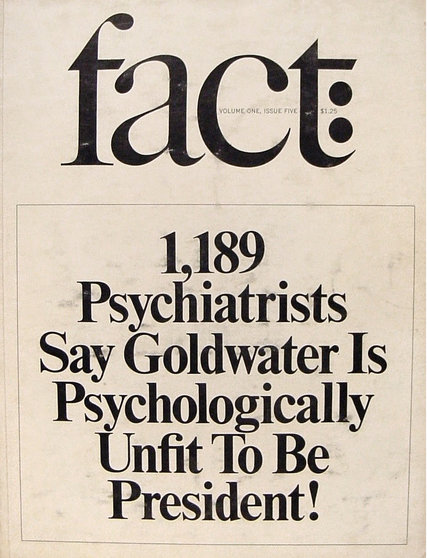
\includegraphics{../images/Goldwater_fact_magazine.jpg}
\end{center}
 \caption{Cover of Fact magazine, 1964. From Wikimedia commons.}
\label{fig: 1964Fact}
\end{marginfigure}


At this same time, you may recall that the US Supreme court decided in 1973 that abortion was covered by the constitutional dictate to a right to privacy, thereby blocking all laws that had kept abortion illegal.

In 1969, the American Psychological Association issued a public proclamation, citing lack of evidence to the contrary that:

\begin{quote}

\textbf{WHEREAS} in many state legislature, bills have recently been introduced for the purpose of repealing or drastically modifying the existing criminal codes with respect to the termination of unwanted pregnancies;

and \textbf{WHEREAS}, termination of unwanted pregnancies is clearly a mental health and child welfare issue, and a legitimate concern of APA;

\textbf{BE IT RESOLVED} that termination of pregnancy be considered a civil right of the pregnant woman, to be handled as other medical and surgical procedures in consultation with her physician, and to be considered legal if performed by a licensed physician in a licensed medical facility.\footnote{Available at http:\slash \slash www.apa.org\slash about\slash policy\slash archive.aspx}
\end{quote}

The American Psychiatric Association followed in 1967 with:

\begin{quote}

The emotional consequences of unwanted pregnancy on parents and their offspring may lead to long-standing life distress and disability, and the children of unwanted pregnancies are at high risk for abuse, neglect, mental illness, and deprivation of the quality of life. Pregnancy that results from undue coercion, rape, or incest creates even greater potential distress or disability in the child and the parents. The adolescent most vulnerable to early pregnancy is the product of adverse sociocultural conditions involving poverty, discrimination, and family disorganization, and statistics indicate that the resulting pregnancy is laden with medical complications which threaten the well-being of mother and fetus. The delivery that ensues from teenage pregnancy is prone to prematurity and major threats to the health of mother and child, and the resulting newborns have a higher percentage of birth defects, developmental difficulties, and a poorer life and health expectancy than the average for our society. Such children are often not released for adoption and thus get caught in the web of foster care and welfare systems, possibly entering lifetimes of dependency and costly social interventions. The tendency of this pattern to pass from generation to generation is very marked and thus serves to perpetuate a cycle of social and educational failure, mental and physical illness, and serious delinquency.

Because of these considerations, and in the interest of public welfare, the American Psychiatric Association

1) opposes all constitutional amendments, legislation, and regulations curtailing family planning and abortion services to any segment of the population; 

2) reaffirms its position that abortion is a medical procedure in which physicians should respect the patient's right to freedom of choice - psychiatrists may be called on as consultants to the patient or physician in those cases in which the patient or physician requests such consultation to expand mutual appreciation of motivation and consequences; and 

3) affirms that the freedom to act to interrupt pregnancy must be considered a mental health imperative with major social and mental health implications.\footnote{Available at http:\slash \slash www.psych.org\slash Departments\slash EDU\slash Library\slash APAOfficialDocumentsandRelated\slash PositionStatements\slash 197703.aspx} ~\citep{Anonymous:1967hr}
\end{quote}

Needless to say, not only were these political events hugely controversial in the United States, the professional involvement of psychiatrists and psychologists was \emph{itself} hugely controversial. 

The `Goldwater affair', as it became to be known, embarrassed Psychiatry as a whole, painting the entire discipline as either politically motivated and unreliable.\footnote{‘Unreliable’ should be read here in the technical sense---the same individual would not be classified the same way by a different analysts)} 

And the declarations regarding abortion were widely seen as unmotivated by scientific evidence.

To this day, academic organizations have a reputation of bias toward liberal political parties. Given that contemporary conservatism traces its root to Goldwater’s failed presidential bid, it is unsurprising that conservative groups may still harbor some suspicion of academia.

\section{Prologue}
\label{prologue}

Your cab pulls up in front of the Shoreham hotel in Rock Creek Park, a particularly tranquil part of the chaos that is Washington D.C. You nervously check the entrance to the hotel. It's clear. This year, there are no throngs of protesters bent on face-to-face confrontation.

They must be down at the mall participating in the massive protest calling for an end to the Vietnam war. The radio reported an estimated crowd of at least 50,000. And that's before the 10,000 National Guardsmen were called into try to open the flow of traffic.

The story was not the same last year, in San Francisco. 

When you arrived at the hotel last year, the entrance was completely blocked by an angry crowd of gay rights activists. Individuals in the crowd were personally confronting—non-violently but aggressively—any member of the APA who appeared. The activists called this `Zapping.' You found it terrifying.

Last year’s conference was almost shut down by the protesters. There are rumors that the FBI was in attendance last year, and it is almost certain they are here now. The Washington Post covered the event thusly:

\begin{quote}

The Washington Post May 14th 1970 -- The gay liberation and their women allies out-shrieked the head shrinkers today and took over an American Psychiatric Association session on sex. Before the morning was over the 500 psychiatrists who gathered to hear scientific studies on sexual problems demonstrated that they were just as prone to anti-social behaviour as anyone else. `This lack of discipline is disgusting', said Dr Leo Alexander, a psychiatrist at the meeting. Then he diagnosed the problem of one of the lesbian protesters: `She's a paranoid fool,' the doctor said, `and a stupid bitch.'\footnote{This is excerpted from a real article in the Washington Post.}
\end{quote}

The conference was a circus. Young men dressed in flamboyant gowns stormed through the hallways. Sessions were disrupted by guerrilla theater. In one, an activist named Frank Kameny grabbed the microphone and shouted “Psychiatry is the enemy incarnate. Psychiatry has waged a relentless war of extermination against us. You may take this as a declaration of war against you.”

It all culminated in a session featuring Irving Bieber, author of the 1962 study on homosexuality published in his book \emph{Homosexuality}.

According to eye witnesses, a protester interrupted Bieber almost before he started with the claim that “I've read your book Dr. Bieber, and if that book talked about black people the way it talks about homosexuals, you'd be drawn and quartered, and you'd deserve it!” ~\citep[p. 200--201]{Clendinen:2013wy} 

Bieber tried to respond by claiming “I never said homosexuals were sick—what I said was that they had displaced sexual adjustment.” 

“That's the same thing, motherfucker!” yelled another.

Earlier this year, a meeting of the New York branch of the APA, a handful of gay activists interrupted a talk by noted Psychiatrist from Columbia University Charles Socarides.

There have long been rumors of a shadow organization of homosexual psychiatrists called the 'Gay-PA.’ It appears these rumors are no longer in doubt. The highlight of this year's program promises to be a symposium titled “Psychiatry: Friend or Foe to Homosexuals: A Dialogue.” The panel includes Dr. Evelyn Hooker, one of the participants in last year's show down and the mysterious `Dr. H. Anonymous,' who claims to be both a licensed psychiatrist and homosexual.

Everyone knows that a mentally ill person cannot practice psychiatry. And homosexuality is a mental illness. This Dr. H. Anonymous, if he or she is telling the truth, is risking his or her medical license. But yet there must be more. We all know, ever since Kinsey's famous study, that about 10\% of the population identifies as primarily homosexual, while a significantly larger percentage have engaged in homosexual activity. And ever since Hooker's paper in 1956, we know that most of this population are psychologically normal. Given the numbers attending this meeting, Dr. H. Anonymous surely can't be alone.

On the other hand, Socarides and Bieber have called Hooker and Kinsey's data into question. If they are correct, and only a small percentage of the population is homosexual, on what basis could one call it a `normal' behavior? Are homosexuals, as Bieber contends, individuals whose “heterosexual function is crippled, like the legs of a polio victim”?
\begin{marginfigure}
 \begin{center}

     
\includegraphics{../images/TimeCover.jpg}
\end{center}
 \caption{Cover of Time Magazine, Oct 31st, 1969}
\label{fig: time1969}
\end{marginfigure}


Back in October of 1969, Time magazine had a cover story on the movement amongst homosexuals---who they called `inverts'\footnote{You can read the entire article here: http:\slash \slash www.time.com\slash time\slash printout\slash 0,8816,839116,00.html\#}---for greater social recognition. In the second paragraph, it referred to “gay” bars (with the quotations), but then proceeded to use the word “gay” without quotes. It even used the term `gay marriage.' The article, however, made the following claim:

\begin{quote}

Most experts agree that a child will not become a homosexual unless he undergoes many emotionally disturbing experiences during the course of several years. A boy who likes dolls or engages in occasional homosexual experiments is not necessarily ``queer'': such activities are often a normal part of growing up. On the other hand, a child who becomes preoccupied with such interests or is constantly ill at ease with the opposite sex obviously needs some form of psychiatric counseling. While only about one-third of confirmed adult inverts can be helped to change, therapists agree that a much larger number of ``prehomosexual'' children can be treated successfully
\end{quote}

Who are these `experts' anyway? Is Psychiatry headed to another embarrassment like the Goldwater affair?\footnote{In 1964, the magazine Fact ran a headline proclaiming that a majority of psychiatrists believed presidential candidate Barry Goldwater mentally unstable. See \fullref{context:theroleofpsychologyandpsychiatryinamericanpoliticallife} for more.}

These thoughts raise a larger specter in your mind: are psychiatry and psychology \emph{scientific}?

Starting a decade ago, Thomas Szasz, Professor of Psychiatry at State University of New York Health Science Center in Syracuse, New York has been arguing, quite publicly, that `mental illness' is a myth! His ideas challenge the very foundation of your field. He's listed on the program, and you're quite excited to get a chance to discuss his polemic claims in some detail.

At the same time, George Miller, who is serving as the President of the APA this year, is something of a revolutionary himself. Miller has been arguing for the existence of something called `Cognitive Psychology', which directly challenges the 50-year tradition of limiting psychological research to the observation, prediction and control of human behavior. For half a century, psychologists have been convinced that they cannot scientifically investigate unobservable entities like ‘beliefs’, ‘desires’, ‘personalities’ and ‘minds’, but rather must study only the behavior of an organism in its environment. Now even that is being challenged!

Are psychology and psychiatry scientific? Is there such a thing as a `mental illness'? Can (or should) science be used to make the world a better place? 

\section{Counterfactuals}
\label{counterfactuals}

In reality there are two distinct associations named `APA.' The American Psychiatric Association, which is composed of Medical Doctors who practice Psychiatry, maintains the DSM. The American Psychological Association, which is composed of academics (PhDs) who study the mind in a variety of ways, does not. 

In this game, I have conflated the two, which is significant transgression according to both sides of the divide. 

If you are interested in studying these events in closer detail, all our characters correspond to a real person or persons. Those with with MDs are members of the American Psychiatric Association, while characters with PhDs are members of the American Psychological Association. 

The American Psychology Association produces a list of educational objectives that are necessary for a Undergraduate Major in Psychology. The first goal “Knowledge Base in Psychology” includes “Identify other fields other than psychology that address behavioral concerns.” Of the eight standard \emph{Introduction to Psychology} textbooks I reviewed\footnote{The instructor’s manual for the game has the full list, if you are interested.}, three (~\citep{Myers:2015ws}, ~\citep{Hockenbury:2014ws} and ~\citep{Zimbardo:2012uz}) mention ‘Psychiatry’ in this context, ranging from a single sentence (~\citep{Myers:2015ws}) to a paragraph (~\citep{Zimbardo:2012uz})---albeit to distinguish Psychiatry from Psychology. Three texts ( ~\citep{Gazzaniga:2018tq}, ~\citep{Cervone:2015ud} and ~\citep{Cacioppo:2018we}) mention ‘Psychiatry’ in later sections where they compare careers in Psychology, and two (~\citep{Lilienfeld:2014ws}, ~\citep{Rathus:2012uz}) fail to mention it at all, at least according to the Index.

For the most part, the historical events with which a character interacts occurred under the umbrella of their respective organization.

\pagebreak 

\chapter{Historical Background}
\label{historicalbackground}

The study of the mind can be traced back to the very foundations of Western civilization in Ancient Greece. For the purposes of this game, we’re going to confine ourselves to the era of ‘scientific’ study of the mind, both in a medical and research context. All historical events up until 1974 that are described in this game book are listed here in a round time line, for ease of reference.

\section{Timeline of events relevant to game play}
\label{timelineofeventsrelevanttogameplay}

Major `eras' are separated for ease of reference.

 \begin{longtable}[!t]{ | P{2cm} | P{11.8cm} | }
\hline
\tahead{Year} & \tahead{Event}  \\ \hline
1792 & Philippe Pinel appointed physician at the Bicêtre hospital in Paris \fullref{foundationinempiricism:phillipepinel} \\
1794 & Pinel appointed chief physician of the Hospice de la Salpêtrière \\ 
1801&Pinel publishes \emph{A Treatise on Insanity}, with his 4-fold classification of mental illness (translated in English in 1806) \fullref{pinelphilippe.atreatiseoninsanity1806} \\
1805&Esquirol published \emph{Mental Maladies}, with a 5-fold classification of mental illness \fullref{mentalalienation-esquirol} \\
1812&George Boole published \emph{The Laws of Thought} \fullref{concurrentdevelopments:logicandcomputing}
 \\
1825&Popular wave of 'homocidal monomania', inspiring (among others) Dostovesky's \emph{Crime and Punishment} \\ \hline
\multicolumn{2}{ | p{13.8cm} | }{\tahead{Empiricism in psychology}} \\ \hline
1847&Helmholtz, Ludwig, Bois-Reyomnd and Brücke vow to develop an account of human and animal behavior that was entirely in physical-chemical terms. \fullref{birthofpsychology:germanphysiologicalpsychologyinthe1880s-1890s.} \\
1850&Fechner first posits that the intensity of a psychological experience had a mathematical relation to the intensity of the physical stimulus (Now known as ‘Fechner’s Law’) \fullref{sensationandperception:fechner} \\
1878&William James contracts to write \emph{The Principles of Psychology} \fullref{americanpsychology:williamjamesandthefunctionofconsciousness} \\
1879&Wilhelm Wundt’s lab at the University of Leipzig opens \fullref{introspection:wundt} \\
1880&Josef Breuer takes 'Anna O' as a patient in Vienna \fullref{hysteriaandhypnosis:freudbreueronannao.} \\
1881&George Beard publishes \emph{American Nervousness}, introducing the idea of a 'nervous breakdown' \fullref{americannervousness---georgebeard} \\
1881&Breuer attempts hypnosis on Anna O. \\
1882&Charcot founds the first clinic on "Incurable" mental illness (what we now call "neurological conditions") at the Salpêtrière in Paris. \fullref{earlyneurology---charcot} \\
1883&Christine Ladd-Franklin completes and publishes her dissertation titled "On the Algebra of Logic" under C.S. Peirce. Johns Hopkins refuses to grant her the doctorate because of her gender.  \\
1885&Hermann Ebbinghaus’ memory experiments call into question the reliability of introspection-based research in psychology, and establishes the paradigm for experimental psychology.\fullref{experimentalism:ebbinghausandtheunreliabilityofintrospection} \\
1885-1887&Charlotte Perkins-Gilman treated for Post-Partum Depression by George Beard's student Silas Wier-Mitchell. \\

1890&A young Sigmund Freud, blocked from a hospital appointment in Germany by anti-semitism, moves to Paris to work under Charcot. \\
1891&The 'neuron doctrine' first advanced by Wilhelm Waldeyer in Germany. \\
1891&Christine Ladd-Franklin leaves Johns Hopkins, where she was denied a PhD because of her gender, to study in Germany with Müller and Helmholtz. \\
1891-1900&Ivan Pavlov conducts research on dog salivation in response to physical stimulus. We now call his method ‘classical conditioning’. \\
1892&Krafft-Ebing publishes \emph{Psychopathia Sexualis} see \fullref{briefhistoryofthestudyofhomosexualityinamerica}, and Appendix \fullref{psychopathiasexualis}\\
1892&G. Stanley Hall appointed 1st President of the American Psychological Association \\
1892&Charlotte Perkins Gilman publishes "The Yellow Wallpaper", based on her experiences with psychological treatment \\
1894&Christine Ladd-Franklin, along with Margaret Washburn, are the first Women to be elected to the American Psychological Association. \\
1895&Freud and Bruer publish their report of Anna O titled "The Psychic Mechanism of Hysterical Phenomena" \fullref{hysteriaandhypnosis:freudbreueronannao.} \\ \hline
\multicolumn{2}{ | p{13.8cm} | }{\tahead{Birth of Psychology as a discipline}} \\ \hline
1896&William James’ \emph{The Principles of Psychology} published. \fullref{americanpsychology:williamjamesandthefunctionofconsciousness}  \\ 

1905&Mary Whiton Calkins elected first woman President of the American Psychological Association \\
1909&G. Stanley Hall invites Freud and Jung to give a series of lectures at Clark University.  In the audience are William James, Franz Boas (anthropology), E.B. Tichner (psychology) and Emma Goldman (the anarchist). After the lectures, Freud and Jung accept an invitation from James Jackson Putnam, a prominent neurologist in New York, to vacation at his home in the Adirondacks.  During this vacation, Freud and Jung have a disagreement, which causes rift between them that never closed. \fullref{theclarklectures} \\
1911&Ramon y Cajal demonstrates neurons in the hippocampus, confirming the 'neuron doctrine' \\
1911&Putnam founds the American Psychiatric Association. \\
1912&Alan Turing born \\
1913&Ebbinhaus’ work translated into English \\
1913&John B. Watson publishes “Psychology as the Behaviorist Views it”, launching Behaviorism. \fullref{psychologysfirstrevolution:behaviorism}  \\
1917&At the inaugural meeting of the American Psychiatric Association, the DSM-I is adopted.  There are 21 mental disorders classified.  \\
1933&\emph{A Standard Classified Nomenclature of Disease} published by the NY Academic of Medicine, along with the Public Health Serve, the Army and Navy Medical Department and the American Hospital Association.  \\
1936&Turing posits the idea of a machine that can compute any mathematical function \\
1939&B.F Skinner publishes \emph{The Behavior of Organisms: An Experimental Analysis}, introducing the concept of ‘reinforcement’ and ‘operant conditioning’ \fullref{operantconditioningradicalbehaviorism:skinner} \\

1939-1945& WWII: significant migration of German researchers to the US; most of the top researchers in the field recruited to the war effort. Large numbers of young intellectuals trained in basic psychiatry for the military. \\
 &Individuals discharged from the US Military for homosexuality begin organic communities in the major ports of the West Coast: San Diego, Long Beach (L.A.) and San Fransisco. \\
1943&bulletin "Medical 203", which defined mental illness for the US military was written by Brigadier General William C. Menninger \\ \hline
\multicolumn{2}{ | p{13.8cm} | }{\tahead{Scientific study of sexuality, and birth of computing}} \\ \hline
1948&Kinsey publishes \emph{Sexual Behavior in the Human Male}  \fullref{thekinseyreport} \\
1949&\emph{The International Statistical Classification of Diseases.} Was published. It had 27 major categories of mental illness and 60 sub-categories \fullref{app: DSMI} \\
1950&Alan Turing publishes “Computing Machinery and Intelligence”, articulating the thesis that the mind can be modeled on a machine, as well as a test for the intelligence of such a machine. \\
1950&The Mattachine Society, in Philadelphia,  and the Daughters of Bilitis, in San Francisco, are founded. \fullref{earlyhomophilemovements} \\
1952&Alan Turing arrested as a homosexual. Is sentenced to chemical castration through hormone therapy. \\
1952&The American Psychiatric Association published the DSM-II, which has 28 major categories of mental illness, and 44 sub categories. \fullref{app: DSMII} \\
June 7th, 1954&Alan Turing commits suicide. \fullref{briefhistoryofthestudyofhomosexualityinamerica} \\
1954&Evelyn Hooker begins her research on the Mental health of male homosexuals in Los Angeles. \fullref{connectingthesethreads:evelynhooker} \\
September 10-12 1956&MIT hosts the second Symposium on Information Theory. In attendance are John von Neumann (the father of computer science), Norbert Weiner (founder of cybernetics), Claude Shannon (creator of Information theory), Warren McCulloch and Walter Pitts (Creators of a mathematical model of a neuron), Margaret Mead (Anthropology), Herbert Simon and Alan Newell (Computer Science), Noam Chomsky (linguistics) and George Miller (psychology). The cognitive revolution has begun. \fullref{thesecondrevolution:cognitivescience}  \\
1955&The Wallace Lab began marketing \emph{Miltown}, the first anti-psychotic medicine.  \\
1957&Skinner publishes \emph{Verbal Behavior}, Chomsky publishes stunning critique. \fullref{chomskyn.reviewofverbalbehaviourbyb.f.skinner1959}\\
1959&\emph{Trofranil}, the first antidepressant, appears on the market. \\
1960&\emph{Librium}, the first anti-anxiety, appears on the market. \\
1963&\emph{Valium} is introduced. \\ \hline

\multicolumn{2}{ | P{13.8cm} | }{\tahead{First street activism in the gay and lesbian community}} \\ \hline
1963&Barbara Gittings becomes editor of the newsletter of the Daughters of Bilitis. \\
1968&Members of the Mattachine society disrupt public lecture by Charles Socarides \\
1969&Oliver Sacks administers L-DOPA to patients comatose since the 1920s, and is amazed to find them awaken.  His memoir 'Awakenings' is published in 1972, and widely read and discussed in the medical community.  \\ \hline
June 28, 1969-July 3rd, 1969&\fullref{stonewall:thestreetactivists} \\
1970&Gay rights protesters picket, and overwhelm, the annual meeting of the APA in San Fransisco. \\ \hline
\multicolumn{2}{ | P{13.8cm} | }{\tahead{Game Begins}} \\ \hline

September 10th, 2009&the United Kingdom issues a formal apology to Alan Turing for his treatment after massive petition drive. \\
Dec 24th, 2013&Turing granted Royal Pardon by Queen Elizabeth II. \\ \hline

\caption{Timeline of critical events}
\label{table: timeline}
\end{longtable}


This events that lead up to the clash over the validity of scientific studies of the human mind span countries and continents. Ideas flow quickly---even in the 18th and 19th centuries, so understanding how the peculiar American definitions of mental health and illness came about require a bit of explanation. 

\section{Brief history of the concept of `Psychology'}
\label{briefhistoryoftheconceptofpsychology}

Psychology is probably the youngest of commonly accepted academic disciplines---the first PhD in Psychology was earned by G. Stanley Hall in 1878. But we'll get to that. First, we have to go back to the notion of science itself.

\subsection{Pre-history of Psychology: Empiricism about the Mind}
\label{pre-historyofpsychology:empiricismaboutthemind}

The scientific investigation into the human mind and\slash or human behavior begins almost simultaneously with science itself. Our inquiry into its history must then begin with the followers of Francis Bacon, who created the ‘scientific method’ and trace the idea that the can be studied scientifically through the rise of the empiricists into the present day. All citations for Bacon are to ~\citep{Bacon:1620ui}.

Bacon, who we now credit with establishing `The Scientific Method,' argued that the human mind tended to distort reality in regular, systematic ways, which he called `idols.'\footnote{The four idols distinguished by Bacon are the idols of the tribe, the cave, the marketplace and the theater. The idols of the tribe are those which we all share, as a function of our biology. They “have their origin either in the regularity of the substance of the human spirit; or in its prejudices; or in its limitations; or in its restless movement; or in the influence of the emotions; or in the limited powers of the senses; or in the mode of impression” (LII)
The idols of the cave are those of an individual. They have their origin in “the individual nature of each man's mind and body; and also in his education, way of life and chance events.” (LIII)
The idols of the marketplace are those of miscommunication and misunderstanding. As Bacon says “For men believe that their reason controls words. But it is also true that words retort and turn their force back upon the understanding; and this has rendered philosophy and the science sophistic and unproductive.” (LIX)
The idols of the theater are those of intellectual `showmanship.' They are “not innate or stealthily slipped into the understanding; they are openly introduced and accepted on the basis of fairytale theories and mistaken rules of proof.” (LXI)
All quotes from Bacon \& Jardin (2000). Roman numerals indicate Aphorism number.} In order to understand reality, we must then give up on the idea that a single person can discover the truth on his or her own.\footnote{For those of you who have read Rene Descartes \emph{Meditations on First Philosophy} will no doubt recognize that Descartes predicated his entire philosophical system on the idea that working alone by pure reflection, he could discover immutable truths about the universe.}

In order to learn about the world, we need to work together, collaboratively creating a “natural and experimental history” (Bk 2, Ch X, p 109) of the phenomenon. As working collaboratively can lead to confusion and misunderstanding, we organize that natural and experimental history into a series of tables: including instances of the phenomenon's presence, closely related instances in which the phenomenon is absent, instances in which the phenomenon occurs in degrees or in comparison, and instances of exclusion of the phenomenon. Once these tables are built, we review them and create what Bacon called a `first harvest' of the phenomenon. In short, this is a generalized axiom unifying the phenomenon yet held close to observation. Once that first axiom is established, we return to the tables, highlighting privileged instances which are further classified as solitary, transitory, revealing, etc.\footnote{Bacon lists 27 different types of these `privileged instances' in Book 2 of his Novum Organon.} These, then can be used to further refine the first harvest into further, more careful axioms.

Bacon profoundly influenced Elizabethan England. His empirical method sparked inquiry in almost all areas of human knowledge, and formed the basis for what we now call the `scientific revolution' or the `enlightenment.' And his influence on psychology and psychiatry is actually far more direct than most would assume. Late in his life, Bacon became friends with the Philosopher Thomas Hobbes. In fact, Hobbes founded a Baconian reading group in Oxford, which is the forbearer of the Royal Society—the world's oldest scientific body.

Thomas Hobbes, who is most widely known for his initiation of social-contract theory in defense of absolute monarchy, opens his master work Leviathan with this bold claim:

\begin{quote}

Nature (the art whereby God hath made and governs the world) is by the \emph{art} of man, as in many other things, so in this also imitated, that it can make an artificial animal. For seeing life is but a motion of limbs, the beginning whereof is in some principal part within, why may we not say that all \emph{automata} (engines that move themselves by springs and wheels as doth a watch) have an artificial life? For what is the \emph{heart}, but a \emph{spring}; and the \emph{nerves}, but so many \emph{strings}; and the \emph{joints}, but so many \emph{wheels}, giving motion to the whole body such was was intended by the artificer? ~\citep[Ch 1, \S 1]{Hobbes:1651wh}
\end{quote}

Just as his famous social-political philosophy posited universal laws of human conduct, Hobbes believed that the human mind followed to universal laws which were deducible through reason. Always a Baconian, Hobbes begins by separating those who have minds (humans) from those who do not (non-human animals), and then query the difference between those two.

According to Hobbes, humans surpass animals in this faculty: “that when he conceived anything whatsoever, he was apt to inquire the consequences of it, and what effects he could do with it.” In addition, humans can “can by words reduce the consequences he finds to general rules, called theorems, or aphorisms; that is, he can reason, or reckon, not only in number, but in all other things whereof one may be added unto or subtracted from another.” ~\citep[Ch V, \S 6]{Hobbes:1651wh}. 

Thus we have the beginning of psychology: human minds work by the process of deducing consequences and abstracting from particular experiences to general rules through basic logical functions. 

Let’s take a moment to contrast this with an alternative approach. René Descartes, who many consider to be the founder of modern western Philosophy, argued that the mind was wholly distinct from the body, and therefore subject to an entirely different set of laws. His most famous argument for mind-body dualism asks us to doubt all that cannot be known with certainty, and then concludes that one cannot doubt that one is doubting; hence thinking; hence one cannot doubt that one is a thinking thing. This famous argument (called the “cogito”) is contained the First Meditation. But Descartes offers a much more interesting and influential argument in a number of other writings. The argument appears twice in \emph{The Discourse on Methods}, first in part 3:

\begin{quote}

{\ldots}if there were such machines having the organs and the shape of a monkey or of some other animal that lacked reason, we would have no way of recognizing that they were not entirely of the same nature as these animals; where as, if there were any such machines that bore a resemblance to our bodies and imitated our actions as far as this is practically feasible, we would always have two very certain means of recognizing that they were not at all, for that reason, true men. The first is that they could never use words or other signs, or put them together as we do in order to declare our thoughts to others. For one can well conceive of a machine being so made that it utters words, and even that it utters words appropriate to the bodily actions that will cause some change in its organs{\ldots} But it could not arrange its words differently so as to respond to the sense of all that will be said in its presence, as even the dullest men can do. ~\citep[Ch 3, 1637]{Descartes:1968uf}
\end{quote}

And then again in part 5:

\begin{quote}

[in looking at the body] I found there precisely all those things that can be in us without our thinking about them, and hence, without our soul's contributing to them, that is to say, that part distinct from the body of which it has been said previously that its nature is only to think. And these are all the same features in which one can say that animals lacking reason resemble us. But I could not on that account find there any of those functions, which, being dependent on thought, are the only ones that belong to us as men, although I did find them all later on, once I had supposed God created a rational soul and joined it to this body in particular manner that I described. ~\citep[Ch 5, 1637]{Descartes:1968uf}
\end{quote}

The same point appears in his \emph{Letter to Henry More}:

\begin{quote}

Nevertheless it has never been observed that any brute beast arrived at such perfection that it could use true speech, that is, that it indicated by words or signs something that can be ascribed to thought alone, and not to a natural impulse. For speech is the only certain sign of thought concealed in the body, and all men, even the stupidest and most insane, make use of it, but not any brute. Therefore, this can be taken to be the true differentia between man and brutes ~\citep[p. 297]{Descartes:ut}
\end{quote}

In these passages, Descartes ascribes to humans alone the ability to use language and conceive of abstract ideas. He then finds that these abilities cannot be the products of material, finite reality. As experience is limited to finite reality, ideas of things that are not finite must be `ascribed to thought alone.' Thus, these ideas must be innate to the mind and not based on experience. It follows that that these distinctly human abilities are the products of a non-material infinite reality. In short, the argument is this:

\begin{enumerate}
\item Humans alone use language and conceive of abstract entities (i.e. `infinity').

\item No material mechanism could ever use language or conceive of an abstract entity.

\item Therefore, humans cannot just be not material mechanism

\end{enumerate}

Hobbes' asserted earlier that human beings could be imitated through material mechanisms, and that our minds are ruled by the law of inquiring of the consequences of an action. This runs directly counter to Descartes' argument, as Hobbes believes abstract entities are merely the result of inquiring consequences. But insofar Hobbes has only made an assertion—a hypothesis—it needs empirical demonstration. To establish Hobbes' contention and meet Descartes' challenge scientifically, Hobbes must show a physical machine could, through experience, develop both the ability to speak rationally and conceive of abstract entities that are not clearly the product of experience (such as `infinity').

It is easy to see how the process of `addition and subtraction' could produce a concept of infinity. But it is hard to see how simple arithmetic could produce a machine that could “arrange its words differently so as to respond to the sense of all that will be said in its presence, as even the dullest men can do.”

John Locke follows Hobbes in this, just as he does in the development of political liberalism. Locke’s famous \emph{Essay on Human Understanding} opens with a fifty-eight page argument against the idea of innate ideas. Locke picks up the project where Hobbes left off, adding `reflection' (what we now call `introspection') as an additional source of ideas. For Locke, like for Hobbes , the mind is populated with ideas that originate in experience. We come to understand our minds, and how our minds occasionally lead us astray, by understanding the mental mechanisms that produce ideas from sensation. Abstract ideas like `infinity' are the products of a process of abstraction:

\begin{quote}

Finite then, and infinite, being by the mind looked on as modifications of expansion and duration, the next thing to be considered, is, -How the mind comes by them. As for the idea of the finite, there is no great difficulty{\ldots}Every one that has an idea of any stated lengths of space, as a foot, finds that he can repeat that idea; and joining it to the former, make the idea of two feet; and by the addition of a third, three feet; and so on, without every coming to an end of his additions, whether of the same idea of a foot, or, if he pleases, of doubling it, or any idea he has of any length, as a mile, or diameter of the earth, or of the orbis magnus{\ldots}This, I think, is the way whereby the mind gets the idea of infinite space. --~\citep[Book 2, Ch17]{Locke:1959wj}
\end{quote}

But like Hobbes, Locke fails to explain how language structure could be produced by a finite mechanism.

At the same time Locke was writing in England, Antione Arnaud, a fervent supporter of Descartes' theory of mind, was developing a school of thought in France which we now call the `Port-Royalist' movement. (~\citep{Carr:1996uw}) The Port-Royalists held that the structure of grammar was universal for humans and could be reduced to the laws of logic. Unlike the empiricists Hobbes and Locke, however, the Port-Royalists, who including the great logician and mathematician Pascal, were dualists and theists. (~\citep{Clark1903}) For the Port-Royalists, thought was different from language, although we tend to think in language through force of habit. Pure thought, both in its content and its structure, becomes imperfect when `translated' into an imperfect spoken language. A perfect language, and perfect grammar, would be possible if each word signified unequivocally a single simple idea, and the grammar of speech matched perfectly the `grammar of thought.' 

The empiricists Hobbes and Locke have adequately responded to Descartes’ assertion that ideas about abstract objects could not have their origin in the physical, finite, world. But neither of them have managed to respond meaningfully to the assertion that the ability to put ideas together \emph{in language} cannot be the product of the physical, finite world.

David Hume, the great Scottish Empiricist is really the first to answer this challenge. He took Locke’s argument against innate ideas and married it to the idea of a universal structure of the mind. First, he extending the argument against innateness beyond the concept of the infinite:

\begin{quote}

The idea of God, as meaning an infinitely intelligent, wise, and good Being, arises from reflecting on the operations of our own mind, and augmenting, without limit, those qualities of goodness and wisdom. ~\citep[\S 2, p. 14]{Hume:IGMvPNU2}
\end{quote}

And second, he advanced the thesis that principles of connection between ideas in the mind were regular and hence subject to empirical investigation. In fact, he posited three: RESEMBLANCE, CONTIGUITY in time or place and CAUSE and EFFECT. ~\citep[Part 1, \S  IV]{Hume:IGMvPNU2}

This thesis he believed explained the universality of human language structures:

\begin{quote}

It is evident that there is a principle of connexion between the different thoughts or ideas of the mind, and that, in the appearance to the memory or imagination, they introduce each other with a certain degree of method or regularity{\ldots} {\ldots}Amoung different languages, even where we cannot suspect the least connexion or communication, it is found, that the words, expressive of ideas, the most compounded, do yet nearly correspond to each other: a certain proof that the simple ideas, comprehended in the compound ones, were bound together by some universal principle, which had an equal influence on all mankind.
\end{quote}

Thus, with Hume, we can find the origin of the empirical study of the mind, although `psychology' was not distinguished from `natural philosophy' for at least another century.

It is important to point out here that for these thinkers, the objects of study are \emph{ideas}. The central claims are that there are regular, law-like relationships between ideas themselves, whether they be causal or grammatical. That central claim unites them with early psychology\footnote{There are many instances of this claim in the history of psychology: see, e.g. Wundt, 1876 (p. 175)}. But as we will see, is the challenged in the Behaviorist revolution in the US in the early 1930’s and 1940’s.

\subsection{Birth of Psychology: German Physiological Psychology in the 1880s--1890s.}
\label{birthofpsychology:germanphysiologicalpsychologyinthe1880s-1890s.}

In about 1847, four friends, three of them students of Johannes Müller (1801--1858), gathered together in Berlin to swear an oath dedicating themselves to undermining vitalism: the theory that all living entities shared a special irreducible ‘vital force.’ They committed themselves to the view that:

\begin{quote}

No other forces than the common physical-chemical ones are active within the organism. In those cases which cannot at the time be explained by these forces one has either to find the specific way or form of their action by means of the physical –mathematical method or assume new forces equal in dignity to the chemical-physical forces inherent in matter, reducible to the force of attraction and repulsion. (Quoted in ~\citep{Bernfeld:1949ji})
\end{quote}

These four friends were Hermann von Helmholtz (1821--1894), Carl Ludwig (1816--1895), Emil du Bois-Reymond (1818--1896) and Ernst Wilhelm von Brücke (1819--1892). They were joined shortly thereafter by Hermann Lotze (1817--1891) and his student Gustav Fechner (1801--1887) and came to dominate the training of the next generation of psychologist and psychiatrists: Helmholtz hired Christine Ladd-Franklin as his assistant, who went on to be one of the first woman members of the APA, and the first woman to hold a professorship at the University of Chicago. Sigmund Freud studied under Brücke; Ivan Pavlov under Ludwig and Wilhem Wundt under du Bois-Reymond. Wundt went on to work in Helmholtz’s lab after Ladd-Franklin returned to America.\footnote{I can illustrate some of the differences in theoretical approach here with the example of color perception: Helmholtz posited that there were three basic primary colors: red, green and purple. Ladd-Franklin argued that purple perceptually appeared to be (i.e. ‘looked like’) a mixture of red and blue, whereas yellow appeared to be primary. Thus, she theorized, there are in fact four psychologically primary colors: red, green, blue and yellow. Helmholtz responded (quoted in Hering) that one could not draw conclusions about facts of physiology from direct psychological experience (i.e. introspection), therefore Ladd-Franklin’s observation had no bearing on the science of psychology. While Ladd-Franklin’s point seems obvious and definitive against Helmholtz’s theory, it was widely rejected, on the basis of the unreliability of introspective reports and observations, in favor of the physiological reductionism of Helmholtz. In fact, it wasn’t until a plausible mathematical model based on Ladd-Franklin’s observation was proposed by Jameson and Hurvich in 1957 that the psychological community rejected Helmholtz’s theory in favor of Ladd-Franklin’s.}

While all four of these thinkers had a profound influence on the founding and development of psychology as a discipline, we’ll focus attention for the moment on Helmholtz\footnote{Experienced Reactors may recognize Helmholtz’ name from the Darwin Game.}. 

Helmholtz was one of the great scientific minds of his era. Not only is he now recognized as a godfather of experimental psychology, he is widely respected in the history or Optics, and is, in many ways, the father of ophthalmology, having invented the ophthalmoscope.

His professor, Müller, held that nerves had `specific sense energies' naturally: our sensory system had certain \emph{a priori} assumptions\footnote{\emph{a priori} is a philosophical term meaning ‘prior to experience.’ It is frequently used to describe philosophical positions like Descartes’ that believe knowledge can be gained by reflection alone. In this case, it means that the nerves have assumptions about the world ‘built in’ before experience. If you wanted to use a computer analogy, Müller believes that knowledge about time and space is encoded in our hardware, where the empiricists like Hobbes, Locke and Hume believe it is in software that is built through experience.} about time and space literally built into them, making sensory experience like binocular vision possible. Students familiar with the history of philosophy may recognize this as a position influenced by Kantian psychology.

Helmholtz, however, posited that our mental system as a whole adjusted itself through a process of `unconscious inference' to represent the external world. The contents of our experiences---the redness of a red apple, for example---are merely `signs' or `indicators' of the objects in the world that our experiences represent. Our sensory systems automatically and unconsciously \emph{recover} the world through the complex information to which it has access. 

Unconscious inferences that produce stable representations (I.e. experience of a red apple) are \emph{not} accessible to us through mere reflection, but neither are they ‘built in’ or ‘innate.’ They are, in short, trained through experience with the regularities of the world itself. The process of sensation is learned, not biologically determined. While contemporary psychophysics has advanced greatly since 1850, the basic model of how perception works in psychology today is Helmholtz's.

\subsection{Major areas of research during the infancy of psychology}
\label{majorareasofresearchduringtheinfancyofpsychology}

\subsubsection{Sensation and Perception: Fechner}
\label{sensationandperception:fechner}

On the morning of 22nd of October, 1850, a young physiologist named Gustav Theodor Fechner lay in bed, puzzled by the relationship between the intensity of a psychological experience (i.e. hearing a sound, measured by introspection) and the intensity of the physical stimulus (i.e. the amplitude of the air vibrations). On that morning, it occurred to him that the relative increase in the physical stimulus might correspond to the relative increase in the psychological experience. It took him a decade to prepare the idea for publication, which he presented as `Weber's law':

\[ dp  = k(dS/S) \]

where dp is the change in the psychological experience, k is a constant to be determined experimentally, dS is the change in the stimulus and S is the stimulus. He added to this the idea that the physical stimulus must break a certain threshold to be perceivable at all to derive what is now known as 'Fechner's law’:

\[ p = k\ln(S/S_{0}) \] 

Where S0 is the threshold under which the stimulus is not perceived.

Fechner's law is the first mathematical law (some might say `model') in psychology. It posits a specific relationship between a psychological entity (sensation) and a physical entity (the stimulus). Unlike his predecessors who had contented themselves with discovering the relationships between ideas in a rather imprecise way, Fechner had both bridged the divide between the psychological and the physical, and given that bridge the precision of Calculus. 

Fechner's book, Elements of Psychophysics, published in 1860, had a profound effect in both Germany and England. Physiologists now had a model of precision for which they could strive. And psychologists had a model of understanding the relationships between the physical and the psychological. Most importantly, however, the book inspired Hermann Ebbinghaus to begin studying memory. But that story will have to be left to another time.

\subsubsection{Introspection: Wundt}
\label{introspection:wundt}

Today, we generally consider Wilhem Wundt's lab at Leipzig to be the first true psychological laboratory. Helmholtz's lab, it is argued, was a lab of physiology, not psychology. But that distinction can be argued over. Wundt, unlike Helmholtz, believed that the causal relations governing ideas and experience were of a different \emph{kind} than those governing the physical world. And it was the challenge of psychology to discover those laws and observe those regularities.

Wundt was, however, a student of Helmholtz. He didn’t run off an join Descartes in reflection. Rather, he believed that the proper explanation of the laws of psychology would make use of the properties of the central nervous system. In Wundt's own words:

\begin{quote}

Physiology and psychology cover, between them, the field of vital phenomena; they deal with the facts of life at large, and in particular with the facts of human life. Physiology is concerned with all those phenomena of life that present themselves to us in sense perception as bodily processes, and accordingly form part of that total environment which we name the external world. \textbf{Psychology, on the other hand, seeks to give account of the interconnection of processes which are evinced by our own consciousness}, or which we infer from such manifestations of the bodily life in other creatures as indicate the presence of a consciousness similar to our own. (1902, p. 1)
\end{quote}

Shortly thereafter, he asserts that Psychology is “\textbf{the investigation of conscious process in the modes of connection peculiar to them.}” ~\citep[p. 2]{Wundt:1902vf}) As consciousness is a unique phenomenon in this world, it can only, then, be approached with the investigative tools unique to consciousness: direct experience of consciousness by ourselves of inferred in others on the basis of direct observation and analogy. This does not mean, however, that a science of psychology is purely introspective. On the contrary, Wundt proposed a `physiological psychology': a theory of conscious experience informed by our physiological understanding of the brain, what Wundt calls the `bodily substrate of mental life.'

The nervous system was thought to be made up of a `central substance' that maintained an equilibrium and `nerve-fibres' that connected cells together. This `central stuff' was understood not to just transmit information, but to modify it in one of two ways: first, if it were exposed to repeated stimulus, the amount of energy needed to produce a response would decrease, and second, in some cases, it could invert the signal into it's opposite (i.e. from `x more than equilibrium' to `x less than equilibrium'). Wundt sought to reduce Hume’s four standard `Laws of Association' of ideas—similarity, contrast, spatial and temporal contiguity— to simple `internal connection', as `contrast' is a completion of an idea in the same way `similarity' is; and contiguity in space and time are external, not internal, relationships. Ideas tend to produce their contrasting idea, rather than ideas which are similar, when they are accompanied by strong feelings, as all feelings have a kind of `elasticity' to them, always presenting with its opposite feeling implicitly.

`Internal connection,' is then is explained by what Wundt called `central innervation,' or the properties of the nervous system. ~\citep{Wundt:1876vu} It is a fundamental law of neuroscience, even then, that `neurons that wire together fire together.' For Wundt and his followers, the similarity and contrast of ideas was explainable by the excitation and inhibition properties of these nerves.

\subsubsection{Behavior: Pavlov}
\label{behavior:pavlov}

Ivan Pavlov was, like the others in this section, a physiologist first. His interest in psychology was, for the most part, tangential to his work in physiology. Between 1891 and 1900, Pavlov conducted a series of experiments on salivation in dogs. His primary interest at this time was to explain why dogs salivated when presented with food at a distance. The common-sense psychological explanation, of course, is that the dog wants the food. Or even that the dog \emph{imagines} or \emph{anticipates} having the food. More technically, early psychologists would have said the dog \emph{associates} food and saliva. But these are not physiological explanations, and they would not satisfy Pavlov.

Using a recently invented apparatus, Pavlov was able to measure the amount of saliva dogs produced in response to a food stimulus. After a number of experiments, Pavlov noticed that the dogs were salivating without any food present. It occurred to him that in these case, the dogs' salivation response might be responding to the lab techs, rather than food itself. To test this hypothesis, he presented food to a dog and simultaneously rang a bell. After repeated exposures to this combination of stimuli, Pavlov removed the food, leaving just the bell. He found that the dogs still salivated.

Thus, Pavlov discovered what came to be called `classical conditioning': to train a behavior, one presents a new stimulus (the conditioned stimulus) concurrently with the stimulus that `naturally' produces the desired behavior (the unconditioned stimulus). After repeated training, the desired behavior (conditional response) will occur with the new (conditioned) stimulus, without the presence of the original, `natural,' unconditioned stimulus.

Pavlov's primary application of his findings were to the nervous system as a whole as well as “heart, digestive tract and other organs in the higher animals” (lecture 23), he didn't shy away from suggesting that it could be used to explain the seemingly involuntary habitual actions of those deemed `psychotic' or `neurotic.' Conditional responses were, however, breakable, or in behaviorists terms `extinguishable,' if one conditioned a new stimulus in place of the existing stimulus-response association.

Pavlov placed particular emphasis on the idea that his experiments were purely objective and not open to observer influence, such as the experiments of the Wundt and his ‘introspectivists.’ In fact, he closes his 1927 lectures with the bold claim that:

\begin{quote}

all the experiments, those of other workers as well as our own, which have set as their object a purely physiological interpretation of the activity of the higher nervous system, I regard as being in the nature only of a preliminary inquiry, which has however, I fully believe, entirely justified its inception. We have indisputably the right to claim that our investigation of this extraordinarily complex field has followed the right direction, and that, although not a near, nevertheless a complete, success awaits it. ~\citep{Pavlov:1946ws}
\end{quote}

The importance of Pavlov's theorizing should be obvious at this point: classical conditioning provided a physiological law-like relationship that could take the place of (provide the bodily substrate for) the association of ideas. And it provides a mechanisms for creating, intervening in, or destroying those associations—which no previous theory had managed to do thus far.\footnote{I am skipping, for the sake of space, the fascinating history of British psychology during this period, as it adapted associationism to the new physiology. See ~\citep{Daston:1978vx}}

\subsection{American Psychology: William James and the function of consciousness}
\label{americanpsychology:williamjamesandthefunctionofconsciousness}

During this period of profound growth and advancement of psychology in Germany, American Universities were not institutions of research, but institutions of education. Starting in about 1876, that started to change. Johns Hopkins University was founded in Baltimore in 1876 with the explicit mission of ``The encouragement of research; the encouragement of young men; the advancement of individual scholars, who by their excellence will advance the sciences they pursue, and the society where they dwell.''\footnote{Daniel Coit Gilman, the first President of Johns Hopkins, admired not just the German University, but what he called the ``German Mind'' as well: “The thoroughness of the German mind, its desire for perfection in every detail, and its philosophical aptitudes are well illustrated by the controversies now in vogue in the land of universities.”(http:\slash \slash webapps.jhu.edu\slash jhuniverse\slash information\_about\_hopkins\slash about\_jhu\slash daniel\_coit\_gilman\slash )} 

Of the 53 men appointed to the faculty of Hopkins by 1884, nearly all had been educated at German Universities, and 13 held what was then a German degree, the “PhD.” The few exceptions to this rule were the eminent American pragmatists John Dewey and C.S. Peirce. 

What followed can only be described as an explosion in research universities in America. Clark University was founded in 1887 and the University of Chicago in 1892. In 1860, no PhDs were awarded in America. By 1890, 164 PhDs had been given. The first of these in ‘Psychology’ was given to G. Stanley Hall by Harvard in 1878.

I mention all of this because the German understanding of the science of the mind---specifically that of Helmholtz and his anti-vitalists---became synonymous with the understanding of research in Psychology during this period. In short, if one approached the mind in some fashion other than this experimental tradition, it simply was viewed as not contributing to research, and hence, was not considered suitable for graduate instruction. More often that not, advocates for views not in accordance with physiological-psychology were restricted to departments of philosophy or anthropology. A particularly good example of this kind of reasoning is G. Stanley Hall’s 1879 paper ‘Philosophy in the United States,’ in which he laments American Philosophy as little more mental discipline and moral training in the Christian tradition.

In the middle of this storm sits William James. James, in many ways, bridges the divide between the older approach to liberal education and the new approach to research as a function of the university. James himself accredits his interest in Psychology to his time spent in Germany, yet his entire career was spent teaching at the traditional college: Harvard. He advocated for experimentalists, but appeared to perform no psychological experiences himself. His students are the major figures in this first generation of research institutions and Psychology departments, including G. Stanley Hall; yet his position was always in the department of Philosophy, something he appeared to have insisted upon.\footnote{See Ch. V of ~\citep{Miller:1962vk}} James had a life-long friendship with the two Hopkins pragmatists, C.S. Peirce and John Dewey, who went on to supervise Christine Ladd-Franklin at Hopkins.\footnote{George Miller argues argues that “If Watson had not been so inept as a philosopher, he might have offered behaviorism as a pragmatic theory of mind, comparable to Peirce’s pragmatic theory of meaning, James’ pragmatic theory of truth, and Dewey’s pragmatic theory of value.”~\citep[p. 66]{Miller:1962vk}} Moreover, James was in frequent contact with the early British philosophers of mind including Alexander Bain, Herbert Spencer and John Sully. 

In 1878 James contracted with Henry Holt and company to write a textbook for this nascent field of psychology. The resultant book The Principles of Psychology is a classic in the field. In it, James defines psychology as “the science of mental life, both of its phenomena and of their conditions” ~\citep[p. 1]{James:1890wm}) and identified introspection as its chief method.

James held that consciousness (which was the central phenomenon to be studied by psychology) was like stream, encompassing much more than mere ‘associations’ of ideas. The associationists who followed Hume isolated experiences from their context, and provided a overly simplistic account. The object of study of psychology---the relations, tendencies and emotions that make up the stream of consciousness---are experienced directly in introspection, and form the basis of genuine scientific inquiry into the mind.

James' fellow pragmatists Peirce and Dewey went on to construct a theory of psychology focused on the functions of mental states, what was called ultimately called “The Chicago School.”~\citep{James:1904dz} Dewey argued that explanations of human activity that focused merely on the `stimulus' and `response' or the British thinker W.K. Clifford’s ‘reflex arcs' were inadequate characterizations of conscious states. In order to truly characterize, and then study, conscious states, science must take into account the function or end of those states. In his words:

\begin{quote}

the distinction of sensation and movement as stimulus and response respectively is not a distinction which can be regarded as descriptive of anything which holds of psychical events or existences as such. The only events to which the terms stimulus and response can be descriptively applied are to minor acts serving by their respective positions to the maintenance of some organized coördination. The conscious stimulus or sensation, and the conscious response or motion, have a special genesis or motivation, and a special end or function. The reflex arc theory, by neglecting, by abstracting from, this genesis and this function gives us one disjointed part of a process as if it were the whole. ~\citep[p. 370]{Dewey:1896vt}
\end{quote}

Functional psychology thus emphasizes the role mental entities play in an organisms behavior, not what those ideas represent, or the `content' of those ideas.~\citep{Dewey:gu}~\citep{Dewey:1916tl}

\subsection{Experimentalism: Ebbinghaus and the unreliability of introspection}
\label{experimentalism:ebbinghausandtheunreliabilityofintrospection}

In or about 1878, inspired by Fechner's stunning results investigating sensation, Hermann Ebbinghaus started experimenting with memory.\footnote{See \fullref{theparadigminexperimentalpsychology:hermannebbinghaus} for more on Ebbinghaus’ experiments. ~\citep{Ebbinghaus:1885ud}} Ebbinghaus sought, like all of his contemporaries, to understand the association of ideas. But he was worried, rightfully so, that using existing words or concepts in an experimental design would allow for the individual subject's previous experience with those words or concepts to influence the result of the experience. Thus, to isolate the association of ideas from any prior influence, he created long lists of nonsense syllables (VAM, ZOK, etc.) and set about memorizing them. He then precisely measured the number of repetitions or amount of time it took to repeat list perfectly, something he called trials to criterion. As it turns out, the longer the list, the more time, or trials, it takes to memorize it. But that wasn't all: he further tested the process of forgetting.

After some arbitrary period, Ebbinghaus would return to the same list and restart the entire process. If it took him the same number of repetitions to memorize the list to perfection, his forgetting would have been complete. What Ebbinghaus found was that even if he could not introspectively recall items on the list after some time, it took fewer repetitions for him to learn the list to the criterion or perfection. Thus, a decade before Freud made it fashionable to believe in the unconscious, Ebbinghaus had demonstrated empirically that the mind could retain information that it could not bring to subjective, introspective awareness.

This discovery was a bombshell to the introspective protocols of Wundt and James. Pavlov had shown that `unconscious' behaviors like salivation could be trained to a stimulus without the intervention of introspection, but Ebbinghaus showed that a paradigmatic psychological phenomenon—memory—was subject to the same training. While Ebbinghaus' work was originally published in 1885 in German, it was not published in English until 1913---which ’just happens’ to be the same year James Watson declared the beginning of the Behaviorist revolution.

\subsection{Tichener---The Structure of Consciousness}
\label{tichener---thestructureofconsciousness}

E.B. Tichener was British psychologist who earned his Doctorate under Wundt’s direction in 1892. He emigrated to the US for a position at Cornell University in Ithaca, NY. For Tichener, Psychology was “\emph{science of mental processes}” ~\citep[p. 5]{Titchener:1896tr}. The term ‘mental’ should give us a little pause. 

Jump back, for a moment, to René Descartes. In \fullref{pre-historyofpsychology:empiricismaboutthemind}, we discussed Descartes’ argument for the existence of the mind as separate from the body on the basis of language and language use. 

Titchener’s definition of ‘mental’ follows in the Cartesian tradition of introspectability: “A mental process is any process, falling within the range of our experience, in the origination and continuance of which are ourselves necessarily concerned.” ~\citep[p. 5]{Titchener:1896tr} Psychology is the science f the ‘mind’ insofar as we understand ‘mind’ to be the sum total of mental processes experienced by an individual over the course of a lifetime. 

\emph{The} problem of a Psychology is

\begin{quote}

(1) to analyze concrete (actual) mental experience into its simplest components, (2) to discover how these elements combine, what are ht flaws which govern their combination and (3) to bring them into connection with their physiological (bodily) conditions. ~\citep[p. 12]{Titchener:1896tr}
\end{quote}

As science begins with analysis---breaking up phenonema into its component parts\footnote{Students who have read Descartes ‘methods’ will no doubt recognize his continuing influence on Titchener’s thinking.}---the first task is to divide and separate mental processes until we arrive at the base unit of analysis: the mental experience. Laws for combining and associating these experiences are then introduced, and the connection thereof to the physical body.

For Titchener, the fundamental unit---the ‘atom’, as it were---of psychology is sensation. Sensation comes to experience fully formed, and cannot be further divided\footnote{Much of Titchener’s work looks, to the contemporary reader, more like philosophy and phenomenology than psychology.}. Sensation is inherently personal, as no one can directly observe another’s sense experiences. Investigating sensation therefore requires introspection. But this does not mean it is unscientific. Indeed, introspection can be performed in reliable ways that would allow for replication by others:

\begin{quote}

\emph{Have yourself placed under such conditions that there is as little likelihood as possible of external interference with the test to be made. Attend to the stimulus, and, when it is removed, recall the sensation by an act of memory. Give a verbal account of the processes constituting your consciousness of the stimulus.} ~\citep[p. 36]{Titchener:1896tr}
\end{quote}

Titchener’s influence on psychology was two-fold. First, he had a student, and devotee, named E.G. Boring. Boring published his \emph{History of Experimental Psychology} in 1929. As the first history of psychology, it largely shaped how Psychology understood itself, enshrining Tichener’s views on science as analysis and sensation and perception as the starting point in Psychology for generations. Second, Titchener’s insistence on Wundt’s introspective method as \emph{the} starting point for Psychology sparked the first revolution: behaviorism.

\subsection{Psychology’s First Revolution: Behaviorism}
\label{psychology’sfirstrevolution:behaviorism}

John B. Watson (1878--1958) opens his 1913 manifesto “Psychology as the Behaviorist Views it.” with the bold claim that \textbf{Psychology}

\begin{quote}

“\textbf{is a purely objective branch of natural science.} Its theoretical goal is the prediction and control of behavior. Introspection forms no essential part of its methods, nor is the scientific value of its data dependent upon the readiness with which they lend themselves to interpretation in terms of consciousness. The behaviorist, in his efforts to get a unitary scheme of animal response, recognizes no dividing line between man and brute. The behavior of man, with all of its refinement and complexity, forms only a part of the behaviorist's total scheme of investigation.” ~\citep[p. 158]{Watson:1913tq}
\end{quote}

In a 1929 debate with the Harvard professor and physiological-psychologist William MacDougall (1871--1938), Watson anticipated a common criticism of behaviorism: that it cannot explain our rich interior mental life---what William James called the “stream of consciousness.” Watson responded that if we were to take the inner mental life as the object of study, rather than observable behaviors, there would be “as many analyses as there are individual psychologists. There is no element of control. There is no way of experimentally attaching and solving psychological problems and standardizing methods.” Thus, psychologists must limit themselves to “things that can be observed, and formulate laws concerning only the observed things.” ~\citep{Watson:iMwU-3B8}

According to Watson, ‘observable things’ includes only “what the organism says or does,” which must then be described “in terms of ‘stimulus and response.’” By ‘stimulus,’ Watson means “any object in the general environment or any change in the physiological condition of the animal, such as the change we get when we keep an animal from sex activity, when we keep it from feeding, when we keep it from building a nest. By response we mean that system of organized activity that we see emphasized anywhere in any kind of animal, as building a skyscraper, drawing plans, having babies, writing books, and the like.”

Watson’s behaviorism explains the behavior of all organisms (not just humans) by producing laws of correlation between stimuli and responses. This was a massive extension of the field of psychology, as animals and babies were not able to give introspective reports. Following Pavlov, Watson contends that an organism initially engages is some random behavior (say, a baby squirming) in response to a stimulus. This ‘unconditioned response’ may be biologically determined, but it is not yet a law of psychology. To ‘condition’ a response, one presents the unconditioned stimulus along with a new stimulus repeatedly. Over time, the organism responds to the new, conditioned stimulus with the original unconditioned response. Thus, to explain any given behavior, one must find the conditioned stimulus that is now correlated with the conditioned response.

MacDougall, among others, challenged Watson to explain “thinking” or “thought” in terms of stimulus and response. Watson does not shy away from this challenge:

\begin{quote}

“The increasing dominance of language habits in the behavior of the developing child leads naturally over into the behaviorist's conception of thinking. The behaviorist makes no mystery of thinking. He holds that thinking is behavior, is motor organization, just like tennis playing or golf or any other form of muscular activity. But what kind of muscular activity? The muscular activity that he uses in talking. Thinking is merely talking, but talking with concealed musculature.” ~\citep[p. 464]{Watson:2013ty}
\end{quote}

According to Watson, a child initiates verbal behavior by talking aloud to and about his surroundings. As that behavior is negatively reinforced, it changes to mumbling to oneself, and ultimately to keeping one's lips closed. It follows that thinking is not an activity of the mind\slash brain alone, but a kinesthetic experience of the entire organism—in short, a behavior. Words are, in Watson's view “the conditioned substitutes for our world of objects and acts. Thinking is a device for manipulating the world of objects when those objects are not present to the senses.” ~\citep{Watson:iMwU-3B8}

\subsubsection{Maturing Behaviorism: Tolman and Hull}
\label{maturingbehaviorism:tolmanandhull}

During the middle of the 20th century, behaviorism in American divided roughly into two camps: Tolman and Hull. Edward Chace Tolman (1886 – 1959) initiated the `war' in 1922 by criticizing Watson.\footnote{Today, Tolman is sometimes called a ‘Cognitive Behaviorist’ (see ~\citep{HOLLAND:2008ci}, e.g.) The term was used by Hull’s defender, Spence, to refer to Tolman’s views in 1950. (~\citep{Spence:1950fx}).} Tolman argued that Watson's belief that all human behavior could be explained in terms of “muscle contraction and grand secretion, as such, would not be behaviorism at all but a mere physiology.”\footnote{In the interests of conciseness, I am skipping over the fascinating and under-rated history of Gestalt psychology. I do this with a heavy heart, as it is one of my favorite topics in the history of psychology. Characters who wish to engage with the tradition of behaviorism, however, should pay careful attention to Wolfgang Köhler's presidential address, included in the appendix, for the Gestalt concerns about this period in American Psychology.} ~\citep[p. 45]{Tolman:1922us}

For Tolman, a behavioristic science must answer three major problems: “(1), given the stimulating agency, determining the behavior-cues (2), given the behavior-cues, determining the behavior-object and (3), given the behavior-object, determining the behavior-act.” (p. 51). (1) is the problem of psychophysics, which is adequately solved by Fechner. (2) is accessible, with rewording, by classical conditioning. (3) is the “important problem of motive.” A proper science of behavior must answer all three of these problems. Doing so, Tolman contends, would allow the behaviorist to understand and better elucidate introspection.

Opposing Tolman, Clark Hull (1884 – 1952) contended that in order for a postulate or theorem to be “truly scientific,” it must “take the form of specific statements of the outcome of concrete experimentations or observations.”\footnote{This is only one of Hull's four criteria. The other are: (1) The definitions and postulates of a scientific system should be stated in a clear and unambiguous manner, they should be consistent with one another, and they should be of such a nature that they permit rigorous deductions. (2) The labor of deducing the potential implications of the postulates of a system should be performed with meticulous care and exhibited, preferably step by step and in full detail. It is these deductions which constitute the substance of a system. (4) The theorems so deduced which concern phenomena not already known must be submitted to carefully controlled experiments. The outcome of these critical experiments, as well as all previous ones, must agree with the corresponding theorems making up the system.} ~\citep{Hull:1940tm} Simple classification of behavior are not, themselves, scientific. But neither is talk of such things as motives. Scientific explanations must make use of clear, unambiguous terms that refer to observable behavior. Everything else is simply not considered to be `science.' Hull contends that psychology should produce mathematical equations that would specify precisely all the relationships between variables that account for an organisms behavior. The specific behavior of a given organism would be an instance of these universal mathematical generalizations.

Hull's primary contribution to behaviorism is the thesis that that the when a given stimulus has the effect of reducing a biological need, the connection between the stimulus and the response is strengthened automatically. While that statement may seem like a commonsense position today (food given as a reward, e.g.), the important part of it in 1935 was the word of `automatically.' Contrary to the introspectivists or even commonsense, one need not be aware of the satiation of one's physical desires in order to strengthen the association between the conditioned stimulus and the conditional response. In fact, most conditioned associations are not accessible to introspective awareness.

Methodologically, Hull's insistence on the mathematical-deductive structure of theory led to a cadre of young psychologists who were able to represent complex relationships between variables mathematically.~\citep{Hull:1940tm} Many members of that generation ended up at Stanford, ultimately providing much of the theory of information processing that allowed the cognitivists to advance sophisticated mathematical and computer models of cognitive states.

In response to Hull, Tolman argued that simple stimulus-response connections were insufficient to explain behavior: specifically rats running a maze for a food reward. In his famous 1948 paper “Cognitive Maps in Rats and Men,” Tolman presented evidence that showed rats that were allowed to wander around a maze randomly before the beginning of training period learned the maze more quickly than rats that began training without prior exposure to the maze. (~\citep{Tolman:1948kv}) Tolman argued that the best explanation for this phenomenon---and our general intuition about why rats appear to pause before beginning down a specific course---is that the rats have built up a `cognitive map' of the maze through their random explorations. He goes so far as to suggest that the rats had the ability to learn through `Vicarious Trial and Error,' or `imagining' what would happen if they responded to a particular stimulus. For Tolman, this was:

\begin{quote}

evidence that in the critical stages-whether in the first picking up of the instructions or in the later making sure of which stimulus is which-the animal's activity is not just one of responding passively to discrete stimuli, but rather one of the active selecting and comparing of stimuli. ~\citep[p. 200]{Tolman:1948kv}
\end{quote}

One of Tolman's students, Ritchie, constructed further experiments to test the capacity of the rats' cognitive maps. By starting rats on the far side of the laboratory, Ritchie found that the rats tended to navigate not by the direct path to the reward, but to the walls of the room itself. Thus, Tolman contends, the rats' cognitive maps were `strip-like' and `narrow.'

It is this concept—the breadth or narrowness of cognitive maps—that allows Tolman to extrapolate to the human mind, going so far to suggest that we may interpret the various psychological mechanisms posited by psychoanalysts as “narrowings of our cognitive maps due to too strong motivations or too intense frustration.” Thus, racists, sexists, pathological patriots, etc. are individuals with too narrow a `cognitive map.' A healthy mind---and a well educated person---is one who can use reason, i.e. “broad cognitive maps” to

\begin{quote}

“look before and after, learning to see that there are often round-about and safer paths to their quite proper goals-learn, that is, to realize that the well-beings of White and of Negro, of Catholic and Protestant, of Christian and of Jew, of American and Russian (and even of males and females) are mutually interdependent.” ~\citep[p. 208]{Tolman:1948kv}
\end{quote}

\subsubsection{Operant Conditioning \& Radical Behaviorism: Skinner}
\label{operantconditioningradicalbehaviorism:skinner}

Starting in 1938, Behaviorism underwent a radical transformation. In that year, Burrhus Frederic Skinner (1904 – 1990) published The Behavior of Organisms: An Experimental Analysis, in which he introduced the idea of operant conditioning.\footnote{See the section on behaviorism in the `Public Character info' section for more on the difference between operant and classical conditioning.} (~\citep{Anonymous:Auva_WZ2}) Skinner's insight was not entirely without precedent, but rather built upon the concept of `instrumental conditioning' originally introduced by Edward Thorndike (1874--1949). 

According to what is now called `Thorndike's law of effect', if a response is followed closely by a pleasurable experience, it is more likely to be associated with the stimulus than if it is followed by a unpleasurable or neutral experience. Skinner turned this idea into the central explanatory mechanism of behaviorism: rather than the conditioned stimulus occurring simultaneously with the unconditioned stimulus, the conditioning stimulus occurs immediately after the desired behavior as a consequence of the desired behavior. In his own words:

\begin{quote}

Operant behavior usually affects the environment and generates stimuli which is “feed back” to the organism. Some feedback may have the effects identified by the layman as reward or punishment. Any consequence of behavior which is rewarding or, more technically, reinforcing increases the probability of further responding. ~\citep[p. 129]{Skinner:1972wq}
\end{quote}

By introducing the idea of reinforcement of a behavior as whatever makes it more likely that that behavior will occur, Skinner was able to undercut Tolman's (and MacDougall's before him) insistence that a purpose or goal was required to explain the behavior of animals.

As a boy, Skinner was fascinated with mechanisms. Legend has it that he even built a steam cannon out of a discarded water boiler. Extraordinarily intelligent, Skinner found Francis Bacon's works at about fourteen, and became enamored with the idea that Bacon may have written Shakespeare's plays. He majored in English and literature at Hamilton College, where he became famous for elaborate practical jokes. During his time at Hamilton, he expressed significant interest in the authors Joyce and Proust – but also physiological psychologists Pavlov and Jacques Loeb. Legend has it that he met Robert Frost, who encouraged him to become a writer. After that did not pan out, he returned to behaviorism through the work of Bertrand Russell---specifically Russell's comparison between `reflex' and `force' in physics.\footnote{“Gradually it was found that all the equations could be written down without bringing in forces. What was observable was a certain relation between acceleration and configuration; to say that this relation was drought about by the intermediacy of `force' was to add nothing to our knowledge. Observation shows that planets have at all times an acceleration towards the sun, which varies inversely as the square of their distance from it. To say that this is due to the `force' of gravitation is merely verbal, like saying that opium makes people sleep because it has a dormitive virtue. The modern physicist, therefore, merely states formulae which determine accelerations, and avoids the word `force' altogether. `Force' was the faint ghost of the vitalist view as to the causes of motions, and gradually the ghost has been exorcized.” ~\citep[p 495]{Russell:2013wy}}

Inspired by Pavlov's maxim “control the environment and you will see order in behavior,” as well as his passion for inventing mechanisms, Skinner began to create machines that would control behavior of an organism by automatically rewarding the desired behavior and punishing behavior that was not desired.

These successes led Skinner to hypothesize that all animal behavior---including human behavior---resulted from such forces. He delineated four types of operant conditioning: positive reinforcement, negative reinforcement, punishment and extinction, which he studied with mathematical precision. Skinner shifted behaviorism's emphasis from reflexes to regularities of the whole organism, moving from the causal link between stimulus and response to the relationship between the response and its reinforcement.

According to Skinner, this form of behaviorism was the inevitable development of psychology into a full-fledged science. Often pulling on an analogy to the history of physics, chemistry and biology, he argued that `consciousness' and `inner causes' were the remnants of superstition, and human psychology and society could be perfected through the principles of operant conditioning. 

Skinner adamantly insisted that scientific inquiry could not countenance hypothetical unobservable entities. Following Russell, Skinner argued that explaining a given behavior, such as `eating,' in terms of a mental state, such as `being hungry,' was ad hoc, equivalent to the pre-scientific explanation of physical events in terms of vitalistic `forces.' For example, if I explain why a glass breaks by referring to it's fragility, I've really explained nothing at all---I’ve only explained breaking in terms of being likely to break. A genuine explanation of a glass's breaking is in terms of the environmental conditions and events immediately prior to the breaking of the glass. Likewise, explaining eating in terms of `hunger' is hollow, repeating only the likelihood of eating behavior.

Throughout his career, Skinner argued that radical behaviorism alone was the scientific approach to psychology. Theories---including Hull’s---cannot refer to underlying entities. When one objects that paradigmatic sciences like physics postulate unobservable underlying entities such as electrons, Skinner retorts that these are not believed by physics to really exist, but are merely convenient placeholders for the mathematical relationships that hold between observable entities.\footnote{See, e.g. interview with Skinner, p. 39 pf Baars.} A scientist must restrict his or her work to observation, not theorizing. In retrospective appraisal of his own work, Skinner would claim of his work in Behavior of Organisms:

\begin{quote}

The notes, data, and publications which I have examined do not show that I ever behaved in the manner of Man Thinking as described by John Stuart Mill or John Dewey or in reconstructions of scientific behavior by other philosophers of science. I never faced a Problem which was more than the eternal problem of finding order. I never attacked a problem by constructing a Hypothesis. I never deduced Theorems or submitted them to Experimental Check. So far as I can see, I had no preconceived Mode of behavior—certainly not a physiological or mentalistic one and, I believe, not a conceptual one.” (1972, p. 112)
\end{quote}

In the years following, Behaviorism came to utterly dominate American Psychology. By 1960, for example, the standard textbook for experimental psychology, Burton G. Andreas' Experimental Psychology could confidently assert:

\textbf{Psychology seeks to express the laws of behavior.} It makes the assumption that all aspects of behavior, like other natural phenomena, are dependent on the conditions under which the behavior occurs{\ldots} Psychology seeks to describe the dependence of the activities of people or animals on their environments and states of being. Psychology's place is delineated by this particular goal and the specific techniques devised for striving toward it. ~\citep[p. 4]{Andreas:WVE4neKa}

\subsection{Concurrent developments: Logic and Computing}
\label{concurrentdevelopments:logicandcomputing}

In 1812, George Boole (1815--1864) published The Laws of Thought, which is now regularly classified as a classic work in Logic. The opening paragraph, however, suggests a different discipline:

\begin{quote}

The design of the following treatise is to investigate the fundamental laws of those operations of the mind by which reasoning is performed; to give expression to them in the symbolic language of a Calculus, and upon this foundation to establish the science of Logic and construct its method; to make that method itself the basis of a general method for the application of the mathematical doctrine of Probabilities; and, finally, to collect from the various elements of truth brought to view in the course of these inquiries some probable intimations concerning the nature and constitution of the human mind. --- Laws of Thought (1854) Ch1 Para1
\end{quote}

Boole, like his predecessor David Hume, believed that the rules that regulate the human mind were simple, and complex ideas were structured out of simple ones in the same way complex theorems are constructed out of simple axioms via logical transformations.

The history of Logic is of great importance here because in 1950, a brilliant young logician named Alan Turing\footnote{You can read more about the life of Alan Turing, who is one of the greatest, yet least well known, scientists of the 20th century, in the section Brief History of Homosexuality.} proposed a theoretical physical machine that would be capable of carrying out logical functions. That theoretical machine ultimately became the digital computer we know today.

He further proposed that such a machine could be taught to understand human language, and one could test the sophistication of that teaching by a simple empirical test, now known as the `Turing test.' An interviewer would have a conversation with two individuals, one human and one computer, for a period of time. If, after five minutes or so, the interviewer could not tell the difference between the two, we would be in a position of calling the machine a `thinking' machine. Writing in 1950, Turing claims:

\begin{quote}

“I believe that in about fifty years' time it will be possible, to programme computers, with a storage capacity of about 109, to make them play the imitation game so well that an average interrogator will not have more than 70 per cent chance of making the right identification after five minutes of questioning.”
\end{quote}

In short, Turing's ideal machine would `respond to the sense of all that will be said in its presence, as even the dullest men can do.' The challenge set by Descartes and dreamt about by Hobbes, Locke and Hume to create a physical device capable of using language in a productive and systematic way was to be met, at least, theoretically, by a machine, the digital computer.

The question that remains for you, in the course of this game, is whether or not Turing's discovery of the logical functions that meet Descartes' challenge in fact lead to, in Boole's words “probable intimations concerning the nature and constitution of the human mind,” and whether or not those `probable intimations' are scientific in nature.

\subsection{The Second Revolution: Cognitive Science}
\label{thesecondrevolution:cognitivescience}

In 1957, two books were published on the topic of language use by humans. As we have discussed, philosophers of mind have long considered language-use \emph{the} defining characteristic of humanity---the behavior that distinguishes humans from animals and thinking from instinct. The empirical study of language-use therefore, has the potential to quantify, analyze and observe, with scientific reliability, what we are as thinking beings.

In the first, Verbal Behavior, B.F. Skinner explained humans' language use in terms of operant conditioning. Verbal behavior is particularly interesting for the behaviorist because it isn't directly reinforced by the world, but rather mediated by another person via his or her own verbal behavior. In fact, this unique feature comes to form Skinner's definition of verbal behaviors: those behaviors that are `reinforced through the mediation of other persons' (1957, p. 2). He later refines and restricts that definition thus: “If we make the further provision that the `listener' must be responding in ways which have been conditioned precisely in order to reinforce the behavior of the speaker, we narrow our subject to what is traditionally recognized as the verbal field.” (p. 225) This definition, you'll no doubt notice, makes no reference to vocalization, words, sentences, thoughts, phonemes, meanings, semantics, grammar, or anything else typically associated with language-behavior.

The second was Noam Chomsky's first book, Syntactic Structures. Chomsky opens by noting that the set of all grammatical sentences in any given language, while infinite, is not random. There are sentences like `Colorless green ideas sleep furiously' which may have never occurred in English before 1957, but nonetheless are grammatical sentences; while at the same time, there are sentences like `Furiously sleep ideas green colorless' that are not grammatical. He then proposes that an adequate theory of language ought to describe a device that generates all and only the sentences that are grammatical in that language. Any theory that can't generate the set of grammatical sentences simply is not an adequate explanation of human language-behavior.

Central to Chomsky's theory is the thesis that humans differ from animals in their ability to use language. You'll remember from the beginning of this history that that view was shared by Rene Descartes and the Port-Royalists, who used it to argue for the distinction between the soul (mind) and the body. For Chomsky, however, the ability to use language does not entail a non-physical soul. Turing's machines showed that a physical entitled generate new and novel sentences that follow the grammatical structures. Verbal behavior, the defining feature of human psychology, is the ability to structure sentences in new and novel ways via the process of recursion, but that does not mean that human minds are non-physical entities.

Not only do the cognitivists reject the behaviorists conjecture that one can explain human behavior without reference to internal states, they reject the behaviorists rejection of the thesis that there is a dividing like between “man and brutes.”

In 1959, Chomsky published a vitriolic review of Skinner's Verbal Behavior, in which he claimed that not only were Skinner's definitions of reinforcement and conditioning either confused or circular, he argues that empirically, children learn grammar at a higher rate than can be explained by operant conditioning. It is included in the appendix.

In the decade before these tumultuous years, the Macy foundation had sponsored series of conferences that introduced some of great early mathematicians and computer scientists including John von Neumann (father of most computer languages), Norbert Wiener (founder of cybernetics), Warren McCulloch and Walter Pitts (who together created a mathematical model of a neuron, which is the basis for all neural network architecture), Julian Bigelow and Arutuo Rosenblueth (also pioneering cyberneticists) to the great social scientists and psychologists of the day, including the anthropologist Margaret Mead, the Gestalt psychologist Wolfgang Köhler. The goal of these workshops was to investigate the similarities between computational machines and human minds and social structures. Behaviorists almost never attended. While the results from these conferences were minimal, they set the stage for MIT's Second Symposium on Information theory, September 10--12 1956, that forever changed forever the face of psychology. 

At that conference, Alan Newell and Herbert Simon, computer scientists from Carnegie-Melon, presented a simple machine that could do logic proofs and Noam Chomsky presented his idea of a transformative-generative grammar as the basis of language. George Miller writes, in an unpublished paper presented at MIT and repeatedly cited by historians of cognitive science, that he came away from the conference with a sense “more intuitive than rational, that human experimental psychology, theoretical linguistics, and the computer simulation of the cognitive process were all the pieces from a larger whole, and that the future would see a progressive elaboration and coordination of their shared concerns.” Miller recalls Newell telling him “Chomsky was developing exactly the same kind of ideas for language that he and Herb Simon were developing for theorem-proving.” ~\citep{MILLER:1979tt}

And so began “the Cognitive Revolution.”

\section{Brief History of the Study of Homosexuality in America}
\label{briefhistoryofthestudyofhomosexualityinamerica}

While homosexual behavior has appeared throughout human history, the notion of homosexuality as an “orientation” or “personality” is relatively recent. The etymology of the word `homosexual' itself shows the intimate connection between the idea of sexual orientation and the history of psychiatry. According to the OED, the term first appears in print in English in C. G. Chaddock translation of R. von Krafft-Ebing 1892 \emph{Psychopathia Sexualis}. Relevant sections are reproduced in Appendix \ref{app: KraftEbbing1}.

The idea of homosexuality as a lifestyle connected to personality is, in the English speaking world at least, indelibly linked to the public persona of the author Oscar Wilde. While he was studying classics at Oxford, he began advocating aestheticism, the view that aesthetic values trump moral or social values in the understanding of art and literature. Wilde parlayed his success as a playwright into fame, cultivating a flamboyant public personal, known for dressing immaculately and flamboyantly, entertaining wealthy society women and having a sharp wit and his talent at dinner conversation. His masterwork ‘The Portrait of Dorian Gray’ plays with this persona in the characters of XX and Gray himself.

In 1895, he and his companion Alfred Taylor were convicted of acts of `gross indecency'\footnote{In Victorian England, `gross indecency' was defined as sexual acts between men that did not rise to the level of `buggery'.} and sentenced to two years hard labor. Their trial was `the trial of the century' in the English upper-class, and to this day, many of Wilde's personal characteristics inform the common stereotypes of homosexual men, for example, fastidiousness with respect to personal appearance, extraordinary wittiness and social adeptness, esp. with upper-class women, are all traceable to Wilde himself.

The next fifty years were not kind to gay folks. “Treatments” for homosexuals included surgical interventions such as castration, vasectomies, lobotomies, sterilization, clitoridectomies, hysterectomies; chemical interventions such as sexual stimulants, depressants, hormonal injections, and pharmacological shock; psychological interventions included adjustment therapy, psychoanalysis, hypnosis, aversion therapy that included electric shock and desensitization;\footnote{There is a superb website in the UK that is collecting stories of patients, doctors and nurses from this era. All are deeply disturbing, some downright terrifying. See http:\slash \slash treatmenthomosexuality.co.uk\slash . I'll quote just one example here, as it so perfectly illustrates classical conditioning:
“We need to remember that the discussions that went on at Maudsley in the early 50s were constantly searching for ways in which we could understand the relationship between events, so again referring to the ideas put forward by Pavlov, Skinner and Wolpe, if a situation produces anxiety and at the same time there is another even occurring then buy the process of conditioning it's quite likely that the reaction of anxiety will become associated with the unconditioned stimulus. By thinking along those lines it seemed to me that if the process of sexual arousal and gratification is linked with something, it may well become the preferred method of seeking gratification. It seemed to me that if a person wanted to stop being involved in and interested in make figures—so long as he had bisexual potential or interests—we might be able to utilize the other half of the spectrum of potential arousal signals. And, if we did that often enough, he then might be gratified by femininity.”
Form `A Psychological Career', anonymous testimonial from http:\slash \slash www.treatmenthomosexuality.co.uk\slash .} and social psychological interventions patterned on Alcoholics Anonymous like `Homosexuals Anonymous' and others.

One of the saddest stories of this era is that of Alan Turing, who was mentioned in the section above on \ref{concurrentdevelopments:logicandcomputing} on page \pageref{concurrentdevelopments:logicandcomputing}. Turing was one of the greatest mathematicians and logicians of his era, if not the greatest. During WWII, he worked at Bletchley park as one of Churchill's famed code-breakers. His efforts in breaking the German codes lead directly to the development of modern logic and the invention of the electronic computer. He is generally considered to be the founder of both modern cryptography and computer science. While working at Princeton, he became friends with Claude Shannon, who is now recognized as the father of information theory. Quite literally, Turing is to the contemporary information age what Newton was to the age of mechanics, or Einstein the nuclear age.

But Turing was also gay. In 1952, he was prosecuted and convicted for being a homosexual. Sentenced to hormone therapy and stripped of his military clearance (remember, during WWII, he was directly responsible for breaking the German code, created the encryption for the Washington-DC phone line, and was privy to the highest secrets of the war), he committed suicide on June 7th, 1954. In 2009, the British Government started a program of accepting online petitions from citizens of the UK. One of the first to be submitted, and promoted by Richard Dawkins, was a call for an official apology to Alan Turing for unjust prosecution. On 10 September 2009, Prime Minister Gordon Brown issued a formal apology to Alan Turing, stating:

\begin{quote}

It is thanks to men and women who were totally committed to fighting fascism, people like Alan Turing, that the horrors of the Holocaust and of total war are part of Europe’s history and not Europe’s present. So on behalf of the British government, and all those who live freely thanks to Alan’s work I am very proud to say: we’re sorry, you deserved so much better.\footnote{For the full statement, see http:\slash \slash www.number10.gov.uk\slash Page20571}
\end{quote}

During this dark period of persecution, advocates for homosexuals (at this time called `homophile' organizations) focused primarily on changing the stereotypes of the homosexual as a step towards ending the criminalization of homosexual acts as well as the psychological and medical `treatments.' There was little activity within the scientific and academic communities on the issue. 

That all started to change when a young social psychologist named Evelyn Hooker started teaching at UCLA.

During WWII, young men and women who were accused of homosexuality in Pacific theater of operations tended to be discharged from the military in California ports, including San Diego, Long Beach and San Francisco. Many, if not most, of these young people could not return to their hometowns because of their dishonorable discharge from the military. As a result, a organic community of homosexuals began taking shape in many of these cities.

While teaching at UCLA, Hooker became friends with one of her graduate students, Sam Fromm. Sam was gay. In 1943, he challenged her to study `people like him' to determine if they were mentally ill (specifically `neurotic') independently of the biases against homosexuality inherent in the psychiatric tradition.\footnote{You'll recall that Freud and the psychoanalytic tradition that followed him believed homosexuality was a regression fixation caused by an underlying, probably narcissistic, neurosis. See \emph{Introductory Lectures} p. 376--384 and 529--531)} In a 1998 interview, Hooker explained the significance of this phrase:

\begin{quote}

“This bright young man, somewhere in his early thirties, had obviously been thinking about this for a long time. And by ‘people like us’ he meant, ‘We’re homosexual, but we don’t need psychiatrists. We don’t need psychologists. We’re not insane. We’re not any of those things they say we are.” (Eric Marcus, WindyCityTimes-current.pdf, October 31, 2007 • vol 23 no 07)
\end{quote}

During the 1940s, Evelyn Hooker became a trusted `outsider' of the gay community in L.A., but didn't want to conduct research on people she saw as her friends.

\subsection{The Kinsey Report}
\label{thekinseyreport}

In 1948, Alfred C. Kinsey (b. 1894 – d. August 25, 1956) published \emph{Sexual Behavior in the Human Male}. It was revolutionary.

Kinsey and his assistants had interviewed 5,300 white males from all walks of American life. The interviews required up to 521 questions, depending on the interviewee’s experiences. Kinsey reported that a large number of men—up to 45\%—reported having at least one homosexual encounter during his adolescence. These encounters are most frequent at young age, dropping to a stable 10\% of the population by age 20--25. These numbers, Kinsey fears, may not tell the whole story because:

\begin{quote}

The social significance of the homosexual is considerably emphasized by the fact that both Jewish and Christian churches have considered this aspect of human sexuality to be abnormal and immoral. … Social custom and our Anglo-American law are sometimes very severe in penalizing one who is discovered to have had homosexual relations. In consequence, many persons who have had such experiences are psychically disturbed, and not a few of them have been in open conflict with the social organization. ~\citep[p. 610]{Kinsey:1998ur}
\end{quote}

The Kinsey report found that homosexual activity as a common part of male sexual development. Self-identifying as a homosexual, or engaging exclusively in homosexual activity, was found to be more rare. But at 10\%, it was almost twice as high as any previous scientific estimate\footnote{The often repeated statistic that 10\% of any given population is gay or lesbian originates with Kinsey’s study.}. Almost as importantly, Kinsey identified the source of psychic disturbance \emph{not} to be the homosexual activity itself, but the social structures that penalize such behavior.

\subsection{Early `Homophile' movements}
\label{earlyhomophilemovements}

\begin{marginfigure}
 \begin{center}

     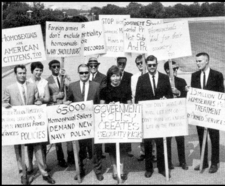
\includegraphics{../images/1965-gay-Picket-thumb-225x186-17508.png}
\end{center}
 \caption{‘Homophile’ activists picketing in 1965. From http://bilerico.lgbtqnation.com/}
\label{fig: 1965Picket}
\end{marginfigure}


Two years after the publication of the Kinsey report, a group of `homophile' activists founded the Mattachine society, which is now generally recognized as the first national gay-rights organization.\footnote{The `Society for Human Rights' was founded in 1924, but never gained national prominence.}

The Mattachine society, named for a European tradition of theater masks, sought to change the prevailing view of homosexuality by presenting the membership as no different than the mainstream heterosexual society. Its members dressed in suits and skirts, and showed no `outward signs' of homosexuality. These `outward signs' are, of course, those stereotypes we identified earlier as originating with Oscar Wilde. Mattachine society demonstrations---held annually in front of Independence Hall in Philadelphia on July 4th---were sober affairs of men in gray suits and women in dresses walking up and down in straight lines, conspicuously \emph{not} holding hands or being affectionate to one another. When couples held hands, one of the leaders of the Mattachine society, Frank Kameny, famously scolded “None of that!” See the ``Rules for Picketting'' published by the Mattachine Society in Figure \ref{fig: MattachineRules}

At the same time, a secret social club for Lesbians called The Daughters of Bilitis was founded in San Francisco by Del Martin and Phyllis Lyon. To stay in touch with its members they created a magazine called `The Ladder', which came under the editorship of Barbara Gittings in 1963. The magazine flourished under Gittings' direction, growing from a simple hand-stapled newsletter to a true 40-page magazine. Gittings became a leader, along with Frank Kameny, of the Mattachine society.

\begin{marginfigure}
 \begin{center}

     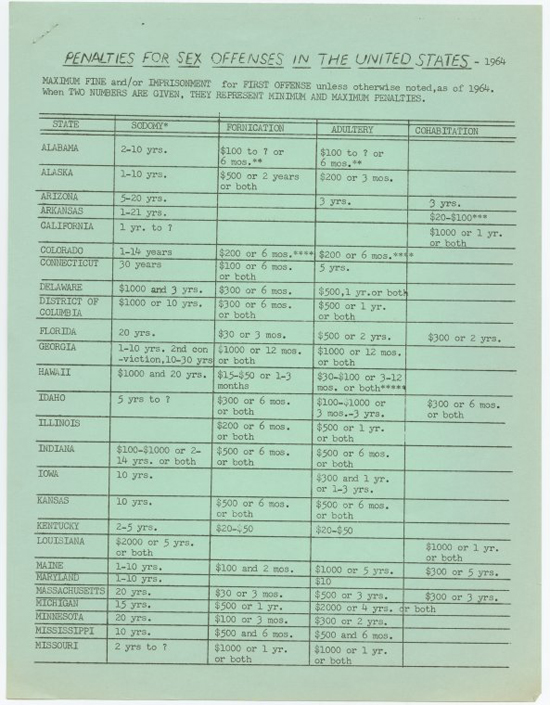
\includegraphics{../PrimarySourceMaterials/MattachineSocietyPamphlet1964-A.jpg}
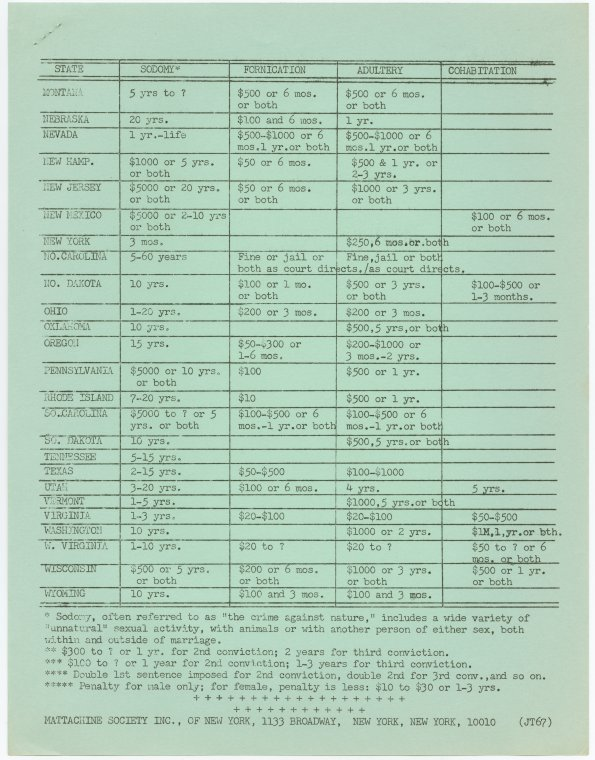
\includegraphics{../PrimarySourceMaterials/MattachineSocietyPamphlet1964-B.jpg}
\end{center}
 \caption{‘Penalties for Sex Offenses’, a Pamphlet distributed by the Mattachine Society in 1964 to educate its members.  From http://web-static.nypl.org/exhibitions/1969/ref/1696842.html}
\label{fig: MattachinePamphlet}
\end{marginfigure}


\subsection{Connecting these threads: Evelyn Hooker}
\label{connectingthesethreads:evelynhooker}

After the publication of the Kinsey report, Hooker finally decided to meet Fromm's challenge. She designed an experiment to determine if homosexuals were mentally disturbed. In 1954, she received a grant from the National Institute on Mental Health to run her study. She recruited 30 homosexuals from the Mattachine society as well as the gay community generally. An equal number of heterosexual men were recruited from civil organizations around the L.A.. Individuals in the groups were matched with respect to age, IQ and education level. All people currently in therapy for mental health were excluded from the study. 

This alone was a major step forward in the study of male homosexuality, as all previous psychological studies had found their subjects in psychiatric wards, army barracks or clinical settings. By studying only those already in psychiatric treatment, one cannot separate traits that may signify an underlying condition from traits that result from the psychiatric treatment itself.

Hooker tested the resulting 60 men using standard psychological tests: the Rorschach, Thematic Apperception Test (TAT) and the Make-A-Picture-Story Test (MAPS). The data was blinded and mixed, and then sent to psychologists with expertise on these the tests who were instructed to score them normally and return the scores. Hooker found no significant difference between the 30 homosexual and 30 heterosexual males with respect to standard tests for mental disturbances, indicating that homosexual men were no more likely to be neurotic than equivalent heterosexual men.

Hooker presented her findings at the 1956 APA in Chicago. Her paper was published in 1957,\footnote{Hooker, Evelyn. ``The Adjustment of the Male Overt Homosexual.'' Journal of Projective Techniques 21(1957): 18--31.} shortly after Sam Fromm's death in a car accident. For more on Evelyn Hooker, see ~\citep{Aldrich:2005wq}

\subsection{Stonewall: The street activists}
\label{stonewall:thestreetactivists}

By the 1960s, tensions were growing in the gay community. Another group of younger gay\footnote{The use of the word `gay' as a replacement for `homosexual' dates from precisely this time with precisely these people. The Mattachine society and the older organizations used `homosexual' and `homophile' to refer to themselves. Ironically, the use of ’Gay' to mean ‘homosexual’ is no attributed to Frank Kameny himself, who started a “Gay is good” campaign in 1968, to parallel the “Black is beautiful” campaign.} activists were growing irritated with both the slow progress of the Mattachine society and its restrictions on behavior. In 1968, a group of young `street-activists' disrupted a meeting of the American Medical Association in New York by shouting down Charles Socarides, a Psychiatrist known for his psychoanalytic treatment of homosexuals.

But everything changed forever on Saturday, June 28, 1969 at 1:20 AM, when the police raided the Stonewall Inn in Greenwich Village. These raids were common---the police would arrest everyone, roughing people up, and generally intimidating the population. But this time, the gay and lesbian patrons of the Stonewall resisted. Events escalated. The riots that followed lasted until Wednesday night, July 3rd. 
\begin{marginfigure}
 \begin{center}

     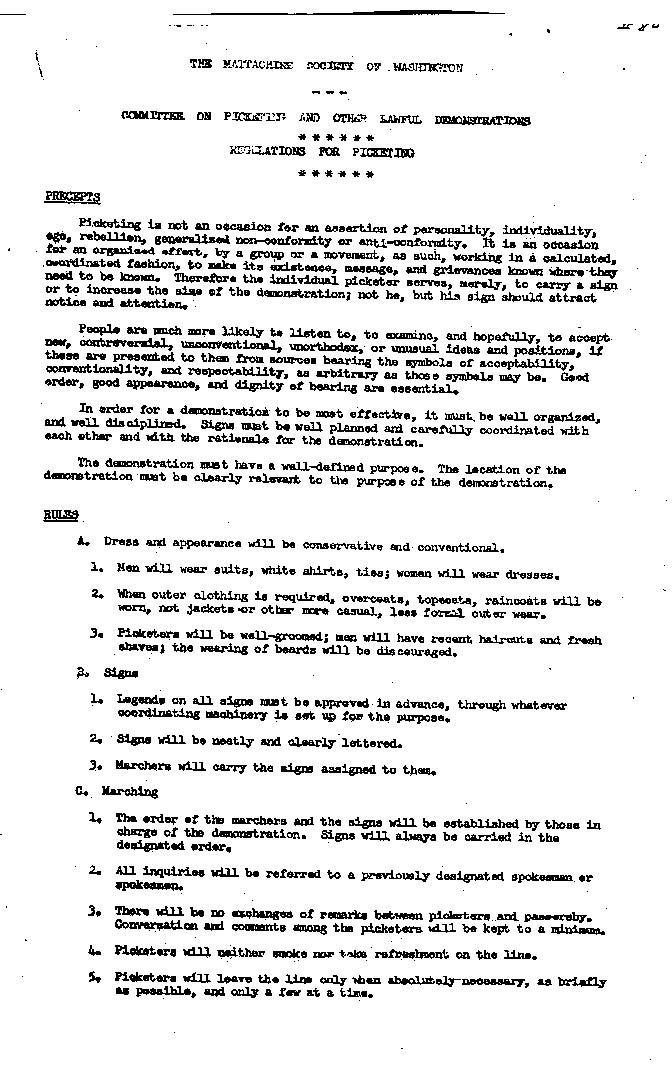
\includegraphics[scale=0.5]{../images/KamenyPicketInstructions.jpg}
\end{center}
 \caption{Rules for Picketing. From the Kameny papers website: http://www.kamenypapers.org/memorabilia.htm, collected 7/14/2016}
\label{fig: MattachineRules}
\end{marginfigure}


On July 4th, the gay community’s attention turned to Independence Hall in Philadelphia and the Mattachine society’s annual march. As usual, Frank Kameny and Barbara Gittings, long time leaders of that gay and lesbian advocacy group, required the women to wear skirts and men suits. But the tide had turned. The young protestors from Stonewall would not conform. Kameny’s approach of assimilation to “straight” behavior had been surpassed by the direct action begun at Stonewall. Militant groups such as the Gay Liberation Front and the Gay Activist Alliance sprouted up overnight (both started in New York). Plans were made to confront those who continued to classify homosexuality as a mental disorder, and directly challenge those who continued to treat homosexuals using barbaric methods.

Those plans included San Francisco, site of the 1970 American Psychiatric Association’s annual convention. And you already know what happened there. (See $<$--\textbackslash{}fullref\{prolouge\}--$>$ if you need a refresher).

\section{Brief History of “mental illness”}
\label{briefhistoryof“mentalillness”}

What makes a certain condition a ‘mental’ condition or a `medical' or ’neurological’ condition? Suppose you are a family doctor, and a patient presents with an unwelcome and unwanted problem---a twitch, perhaps. Do you call a psychiatrist or a neurologist? How do you know?

While behaviors associated with mental illness---hallucinations, catatonic states, mania, etc.---have been known since ancient times, psychiatry dates its regularization as a scientific discipline to the work of the French physician Phillipe Pinel. His \emph{Traité médico-philosophique sur l'aliénation mentale; ou la manie} stands as the first attempt at a scientific classification of mental illness. The book, translated as \emph{Treatise on Insanity} in 1806 by D.D. Davis, is excerpted in Appendix \ref{app: Pinel} on page \pageref{app: Pinel}. 

Pinel was an intellectual disciple of Étienne Bonnot de Condillac, who in turn, was a disciple of John Locke.\footnote{See, e.g. Treatise on Insanity, p. 46} Locke is most well known as the intellectual progenitor of the American Constitution, but his views on the nature of mind and the empirical basis of knowledge held sway over much of the Western intellectual world in the first half of the 19th century. Locke's influence on Condillac and hence Pinel was two-fold: first, he held that all our ideas originate in sensation and reflection. Second, and as importantly, Locke followed Francis Bacon in teaching that all knowledge must be based on careful, systematic observation.

For the empiricists, it follows that insanity, which is a severe form of our ideas `leading us astray', is explained by a incorrect connection and association of ideas. The mechanism is simple: some of our ideas have a natural affinity or connection with one another. Others are held together by mere custom or habit. Cases of insanity are cases where habitual associations become so disorganized they begin to effect the `natural' associations. This misassociation can become so extreme that it can “set us awry in our actions, as well moral as natural, passions, reasonings, and notions themselves” ~\citep[Bk 2, Ch 33, p9. Pg. 531]{Locke:1959wj}. To this day, we use metaphors like `lost his senses' to describe someone with mental illness; and we describe poorly chosen actions as `not very sensible.'

This is simply the theoretical basis for understanding insanity in the broadest possible terms. To truly understand how mental disorder is defined and classified, we must consider how the mentally ill have been treated.

\subsection{Foundations}
\label{foundations}

\subsubsection{Foundation in Empiricism: Phillipe Pinel}
\label{foundationinempiricism:phillipepinel}

Phillipe Pinel (1745--1826) revolutionized the treatment of the insane. When, in 1792, he was appointed a physician at the main asylum in Paris---the Bicêtre hospital---the situation was dire. According to a biographer in 1846:

\begin{quote}

The buildings were unfit for habitation. In them were congregated men crouching together in the mud, in stone cells, narrow, cold, damp, destitute of air and light, and merely furnished with a straw bed, seldom renewed, and soon becoming foul and offensive; wretched dens, in which one would hesitate to place the meanest animal. The insane, who were immured in these filthy holes, were at the mercy of their attendants, and these persons were malefactors released from prison. The wretched patients were loaded with chains and manacled like convicts. Thus given up defenseless to the wickedness of their guardians, they were the sports of an insulting mockery, or of a brutality all the more blind that it was gratuitous. ~\citep[p. 194--195]{Marx:1847vc}
\end{quote}

Upon his arrival, Pinel immediately began advocating pity, respect, and compassion for the patients,\footnote{The story of how Pinel became interested in insanity is frequently retold. Like Newton's apple, it is probably something of a myth, although there may be some core of truth. Here it is, as told by himself in A Treatise on Insanity:
 The loss of a friend, who became insane through excessive love of glory, in 1783, and the ineptitude of pharmaceutic preparations to the mind elated, as his was, with a high sense of its independence, enhanced my admiration of the judicous precepts of the ancients, and made me regret that I had it not then in my power to put them in practice. (p 52)
From a letter by Marx 1846:
 {\ldots}in 1785, he had the misfortune to lose a young man to whom he was much attached, and whose reason became affected through excessive study and abstinence. This unfortunate person, after his return to his family, became maniacal, one evening he escaped from his father's house into the neighboring forest and was devoured by wolves; a few torn rags were found the following day, and near them a copy of the Phaedra covered with blood.
And by Lisa Appignanesi in 2009:
A shy provincial like himself, the friend had fallen into despair and then `mania' when his legal aspirations failed to materialize. Unable to help the younger man once he had all but ceased to eat, Pinel had brought him to the Hôtel-Dieu where a treatment of baths and food seemed to restore him. But his worried family intervened and took him home before he was quite well. The youth escaped their hold, fled to the woods and was found dead only after the wolves had got him. ~\citep[p. 58]{Marx:1847vc}} not only for humanitarian reasons, but also in order to allow the Baconian method of careful observation. Given the terrible conditions at the Bicêtre, Pines argued, one would never be able to determine if the behavior of the patients was the result of some underlying condition, or the condition of the Hospital itself. Bicêtre's chief physician, Pussin, was sympathetic to Pinel's techniques, and began a pilot study of unchaining the patients.

Two years later, Pinel was appointed chief physician of the Hospice de la Salpêtrière---Paris' parallel institution for women. There, the women were kept chained, often naked, in subterranean cells; subjected to the terrors of abusive guards and hungry rats. Pinel immediate banned the use of metal chains as restraints, allowed the women clothing, and established something resembling human civility.\footnote{From a letter of honor, included in Marx 1846: “He who walks in an odoriferous flower-garden, which had formerly been a pestilential swamp, will best be able to appreciate what you effected in madhouses. Formerly an atmosphere almost stifling, damp rooms, the clank of chains, the cries of those under the lash, the hoarse growl of the rough attendants, the desperate frenzy of the ill-used patients; these succeeded by clean apartments, the greatest humanity in personal attentions, and an atmosphere of peace and confidence throughout the whole establishment. ~\citep[p. 210]{Marx:1847vc}} This act was mythologized during the French Revolution as part of the overthrow of the aristocratic order, and has been duly commemorated in Art.\footnote{See Roberty Fleury's `Dr. Phillippe Pinel at the Salpêtrière' (1795)}

Pinel's revolutionary kindness is not just a story of a sympathetic humanitarian. Pinel's goal was to systematical classify mental illness in the Baconian manner. The conditions of confinement found in the Bicêtre and the Salpêtrière compounded the patients' mental illness, and confounded his attempts at observation. In these conditions, one could not determine if the regularity of symptoms found in the population resulted from the illness or the ‘treatment.’ By providing the patients respect and dignity, he believed he could observe their mental illness in a more untainted form.

In general, Pinel followed Locke and Condillac in holding that insanity was 'derangement of the understanding’\footnote{See, e.g p. 3, Section 4, p 134. Also, from the Marx (1846): Every delusion is the result of confused modes of thinking; wrong and crime originate in ignorance.” ~\citep[p. 212]{Marx:1847vc}}, yet extended the view to cover cases where memory, understanding and judgment were perfectly sound, and still the patient was maniacal. 

Pinel thus abandoned any formal all-encompassing theoretical explanation of insanity per se, especially that which originated in Ancient Greek thought. The Greeks, he reasoned, were wrong about how the human brain functions, as we now understood. And as their system was based on their mistaken physiology, it is unreliable. 

Instead, Pinel explicitly bases his system on “the numerous and important facts which have been discovered and detailed by modern pneumatologists” ~\citep[p. 135]{Pinel:1806ws} 

 \begin{longtable}[!t]{ | P{2cm} | P{11cm}  | }
\hline
\tahead{Name}&\tahead{Presentation and Specific Character} \\ \hline 
Melancholia or delirium upon one subject exclusively&Presentation: taciturnity, a thoughtful pensive air, gloomy suspicions, and a love of solitude. (\S 54)\newline  Specific characterization: no propensity to acts of violence, independent of such as may be expressed by a predominant and chimerical idea: free exercise in other respects of all the faculties of the understanding: in some cases, equanimity of disposition, or a state of unruffled satisfaction: in others, habitual depression and anxiety, and frequently moroseness of character amounting even to the most decided misanthropy, and some times to an invincible disgust with life.(\S 59) \\ \hline
Mania without delirium&Presentation: no period do they give evidence of any lesion of the understanding, but are under the dominion of instinctive and abstract fury(\S 60) \newline
May be continued or intermittent. No Sensible change int eh functions of the understanding ; but perversion of the active faculties, marked by an abstract and sanguinary fury, with a blind propensity to acts of violence. (\S 64) \\ \hline
Mania with delirium&Presentation: faculties may be excited by intense or vehement passions, bu exalted and furious enthusiasm, or whatever strong emotions that may originate in fanaticism or chimerical delusion.(\S 60) \newline
May be continued or intermittent, with regular or irregular returns of the paroxsyms. It is distinguished, both in respect to the functions of mind as well as those of the body, by a strong nervous excitement; and marked by the lesion of one or more of the functions of the understanding, accompanied by emotions of gaiety, of despondence or of fury.(\S 67) \\ \hline
Dementia, or the abolition of the thinking faculty&Presentation: extreme volatility, thoughtless absence, extravagant improprieties, and wild eccentricities(\S 68) \newline
Rapid succession or uninterrupted alternation of insulated ideas, and evanescent and unconnected emotions. Continually repeated acts of extravagance: complete forgetfulness of every previous state: diminished sensibility to external impressions: abolition of the faculty of judgement: perpetual activity.(\S 67) \\ \hline
Ideotism&Presentation: partial or total abolition of the intellectual and active faculties.(\S 72) \newline
Total or partial obliteration of the intellectual powers and affections: universal torpor: detached, half articulated sounds; or entire absence of speech from want of ideas: in some cases, transient and unmeaning gusts of passion.(\S 76) \\ \hline
\caption{Pinel’s classification system}
\label{table: pinel}
\end{longtable}


Pinel spent a great amount of time showing that the conditions he was treating did not have a physiological basis. Much of his argumentation in Treatise on Insanity turns on the dissections performed on patients who had died while at the Bicêtre. The reason for this was two-fold: first, the ancient Aristotlean understanding of the mind held that mental illness resulted from too much or too little of one of the four main `humours': black bile, yellow bile, blood and phlegm.\footnote{Each humour had an associated personality type. Imbalance in a given humour was thought to be the cause of imbalances in mood or personality: people with too much black bile were melancholic, yellow bile choleric (full of energy), blood sanguine (impulsive), and phlegm phlegmatic (emotional). See Aristotle's Problems Bk 3, Section1 Galen's De temperamentis, and Avicenna's The Canon of Medicine for more detail.} By showing that the mentally ill had no significant lesions in the brain, or imbalances in their `fluids', Pinel was able to establish the independence of psychiatry from other forms of medicine.

Secondly, there is a long tradition of defining the `mental' as that which is opposed to the `physical'. For example, Rene Descartes famously argues that the actions of our bodies can be explained entirely in physical, mechanistic terms, except that which can be attributed to, in his terms, our `souls.' It follows then, that if an illness is to be truly mental, it must not have a physical explanation. And most importantly, physical causes are treated with physical interventions. As insanity was now deemed non-physical, the treatment cannot be physical. Hence, psychiatry is a discipline independent from physical medicine.

While Pinel had no strong theoretical commitment or agenda, by following Locke's notion of mental illness as a confusion of ideas, he made two significant contributions to both psychiatry as a medical discipline and our understanding of the mind more broadly: First, if insanity was just a misassociation of ideas, it was not a permanent, inherited incurable disease. Second, if insanity is a misassociation of ideas, it does not depend on or result from physiological changes. Explanations for mental illness thus did not require autopsy; and treatment did not require surgery.\footnote{The modern reader of A Treatise on Insanity is impressed by the number of times that Pinel stresses these two features of mental illness. We take both of these for granted to such an extent that the work can seem highly repetitive and redundant. But they were radical theses in the late 18th century, and Pinel's thoroughness in covering the topics no doubt reflects the importance of these thesis in his own mind. (Cite Data – number of pages, examples, etc.).} Psychiatry was, as a result, independent of medicine.

It is likewise important to recognize that Pinel was, in many ways, precisely following Bacon's system of investigation. He was not attempting to form an overarching explanation. He was setting down tables upon tables of observed facts, classifying and arranging phenomena, highlighting privileged instances, and was open to any and all techniques that might shed light on these cases. After initial observation, he split “insanity” into four varieties, distinguishing between the incurable dementia and idiocy from the often transient and curable mania and melancholy.

Therapeutically, Pinel called his humane treatment of the insane the `moral treatment.' In his words,

\begin{quote}

I then discovered, that insanity was curable in many instances, by mildness of treatment and attention to the state of the mind exclusively, and when coercion was indispensable, that it might be very effectually applied without corporal indignity. (p. 108).
\end{quote}

His therapeutic program meant paying attention to the environment in which the insane were confined. He changed the architecture, the diet, the way the nurses and orderlies treated the patients, everything. He even went so far as to allow the higher-functioning patients to work as nurses for the lower-functioning. Patients were listened to. Careful, detailed personal histories were taken. Baths, walking and gardening were encouraged.

A lack of theoretical commitment meant that Pinel could borrow techniques from the many snake-oil salesmen and charlatans who populated Western Europe at the time. One of these fads happened to be mesmerism, now known as hypnosis. We’ll come back to the importance of mesmerism in the rise of psychoanalysis below.

As a follower of Bacon, Pinel was only interested tabulating observations of results, and comparing them against the observations of the condition without intervention. He insisted that we cannot cure a disease until we know of the progression of the disease \emph{without} intervention. In his own words, “We cannot cure diseases by the resources of art, if not previously acquainted with their terminations, when left to the unassisted efforts of nature.” (p. 109). For him, extreme treatments could only be used in extreme cases. The curable would be cured by simple humane treatment.

It is worth pointing out that the word `asylum' means, of course, a sanctuary or refuge. It \emph{first} appears in English in the 1808 translation of Pinel's \emph{Treatise on Insanity}, to reference the Bicêtre. It appears in English newspapers starting in the 1860's, to describe leper colonies---long after Pinel's `moral treatment' had come to dominate the English treatment of the mentally ill.

\subsubsection{Mental Alienation - Esquirol}
\label{mentalalienation-esquirol}

While Pinel tended to think of transient mental illness as a confusion of ideas, he occasionally spoke of the role of passions in mental illness. In the early pages of the Treatise, he hypotheses three different causes of insanity:

\begin{quote}

I now proceed to describe the general progress of periodical insanity. Among its various causes; exclusive of changes in the state of the atmosphere, my experience leads me to enumerate as the most frequent; undue indulgence of the angry passions; any circumstances calculated to suggest the recollection of the original exciting cause of the disease, intemperance in drinking, inanition, \&c. ~\citep[p. 12]{Pinel:1806ws}
\end{quote}

Pinel's greatest student, Esquirol built on this hypothesis of `undue indulgence of the angry passions' and redefined the notion of transient insanity as `mental alienation.' It was Esquirol who grew the empirical understanding of the mind into a full-fledged psychiatric system. But like Pinel, the set of conditions he sought to explain were those with symptoms that were not obviously explained by physical, bodily conditions.

Esquirol split Pinel’s ‘Melancholia’ (see \fullref{table: pinel}, into ‘monomania,’ or obsession with a single idea, and `lypemania.' The latter he renamed partially because the ‘melancholia’ implied the medieval theory of `humors' and 'black bile,’ which Pinel specifically wanted to banish. 

Monomania, lypemania and mania were distinguished by the nature of the passions that are out of order: “The passions of the insane are impetuous, especially in mania and monomania. They are of a depressing character in lypemania. In dementia and imbecility, those only exist, which spring from the first wants of man,--love, anger, jealousy.” ~\citep[p 26]{Esquirol:1845ug} 

As the curable, transient forms of insanity were diseases of malformed passions, their treatment required reforming or redirecting the passions. His five varieties of insanity are defined thus:

\begin{enumerate}
\item Lypemania (melancholy of the ancients) delirium with respect to one, or a small number of objects, with predominance of a sorrowful and depressing passion.

\item Monomania, in which the delirium is limited to one or a small number of objects, with excitement, and predominance of a gay, and expansive passion.

\item Mania, in which the delirium extends to all kids of objects, and is accompanied by excitement.

\item Dementia, win which the insensate utter folly, because the organs of thought have lost their energy, and the strength requisite to fulfill their functions.

\item Imbecility, or idiocy, in which the conformation of the organs has never been such, that hose who are thus afflicted, could reason justly. ~\citep[p. 29]{Esquirol:1845ug}

\end{enumerate}

It is important to note here that the passions \emph{accompany} delirium with respect to collections of objects. One cannot be passionate without being passionate about something. The `something' that is the object of passion is supplied by the senses---and hence, we're still within a Lockean framework of understanding the mind. 

According to the Lockean framework, all ideas originate in sense experience or internal reflection. When the passions directed at one of these ideas becomes excessive and out of control, lypemania or monomania results, depending on the nature of the particular passion that becomes excessive. When the passions are exaggerated without a specific object, and hence apply themselves to every object, or what ever object is before the senses at a particular moment, we call that mania.

Mental illness's causes “are as numerous as its forms are varied.” Case studies presented in his Mental Maladies include climate, seasons, age, sex, temperament, trauma (especially during the first menstrual cycle for young women), excessive study, ambition, etc. Again, as in Pinel, the difference between the mentally ill and the mentally stable is one of scale, not of kind. Everyone has passions---they are why we grieve, fall in love, work for that `A', make personal sacrifices for our friends and families, etc.---the question of insanity is whether these passions are appropriate or excessive and whether they are directed at an appropriate or inappropriate object.

According to Esquirol:

\begin{quote}

“The first wants of man, limiting themselves to those connected with his preservation and reproduction, provoke the determinations of instinct; an internal impulse leads us to gratify them.

The secondary wants, attach themselves to the first, and the desires which they excite, acquire as much more energy, as we have means of satisfying them, They produce the primitive passions; in fine, they are the wants which are connected with our preservation; and are the fruit of our increasing intelligence and civilization. They engender the factitious passions,—those passions which cause the greatest injury to man, especially in the higher walks of life.

Infancy, except from the influence of the passions, is almost a stranger to insanity; but at the epoch of puberty, the sentiments, unknown until this period, cause new wants to arise. Insanity then appears, to trouble the first moments of the moral existence of man.
At mature age, the relations become extended, social wants multiple and the passions take a new character. In proportion as the amorous passions become enfeebled, those of a factitious nature grow strong. Personal interest, ambition, love of distinction and avarice, replace the charms of love and delights of paternity.

At this period of life also, mental alienation appears; insanity is more obstinate, and more concentrated. It passes more readily into a chronic state; and is more dependent upon abdominal lesions.

A sense of his weakness, renders the old man more clam; and while meditating upon the errors to which the passions lead, he isolates himself, and becomes an egotist.

Insanity from a moral cause, rarely exists with him, and when he loses his reason, it is because his organs are fatigued and exhausted. Hence, it is neither mania nor monomania which is developed, at this period, but senile dementia.

Of all moral causes, those which most frequently produce insanity, are pride, fear, fright, ambition, reverses of fortune, and domestic trouble. This last should have been placed, relative to its great influence, at the head of the moral causes, if it be limited to a simple ideas; but by domesticate troubles, I express all the pains, all the griefs, all oppositions, misfortunes and dissensions that grow out of the family state.
~\citep[P. 45--46]{Esquirol:1845ug}
\end{quote}

Esquirol began to gather around himself a `circle' of students who are sometimes referred to as the 'mental alienists.’ Two of the most famous of his students were Charles Lasègue, who is now credited with working out the first definition of hysteria and first documenting \emph{anorexia nervosa}; and Étienne-Jean Georget who delineated four sub-types of `monomania': theomania (religious obsession), ertomania (sexual obsession), demonomania (obsession with evil) and homocidal monomania.

Esquirol's concept of monomania sparked what is probably the first recorded wave of copy-cat psychosis. In November 1825, a young single mother of two named Henriette Cornier, decapitated the 19 month-old child of her neighbors. She had prepared her room for the act, even placing a bucket to catch the blood. She had known the family of the infant for only ten days, and had, up until this event, been nothing but loving and gentle towards the little girl who would be her victim. When the police arrived, she offered no resistance to the police, and did not flee. She confessed, saying that the idea had taken hold of her, and she simply had to act upon it.

The case became a sensation across Europe. Georget diagnosed her as a `homicidal monomaniac.' At her trial, the jury decided that the act had not been premediated and as a result, she was sentenced to life in prison with hard labor instead of death. This ruling makes little sense: Cornier admitted that the idea had occurred to her before the event, and she had carefully prepared her room for the murder. Thus, many commentators---include Lisa Appignanesi ~\citep[p 75]{Appignanesi:2009vl}---have attributed the jury’s leniency to Georget's diagnosis of mental alienation. After all, if Cornier was mentally ill, does pre-planning count as `premediation'?

The idea of the murderous monomaniac took off across Europe, informing or appearing in some of the greatest literature of era, including (according to various literary critics) Poe's “The Tell-Tale Heart,” the character of Roskolvikov in Dostovesky's \emph{Crime and Punishment}, and even Heathcliff in Bonte's \emph{Wutherheights}. The Marquis de Sade is also said to have been a monomaniac.
\begin{marginfigure}
 \begin{center}

     
\includegraphics[scale=0.25]{../images/crimenandpunishment.jpg}
\end{center}
 \caption{Cover of first edition of ‘Crime and Punishment’ by Fyodor Dostoevsky By [Public domain], via Wikimedia Commons }
\label{fig: crimeandpunishment}
\end{marginfigure}
 

\subsection{Early Neurology}
\label{earlyneurology}

Western medicine understood that the nervous system used, or conducted, electricity from the Galvani’s famous frog-leg experiments of 1780. There were, as one might expect, different interpretation of the relationship between nerves and electricity---Galvani believed electricity was the ‘vital force’ contained in living things\footnote{And hence, the frequently-used trope of science fiction dating back to Frankenstein that the dead can be brought back to life with electricity.}. Galvani’s colleague Volta, who went on to lend his name to the ‘Volt’, argued that the frog leg reacted to electricity, but did not contain it.
The precise relationship between nerves and electricity, as well as the relationship between the nervous system an our psychology, was not nailed down for a long time. But that didn’t stop researchers in this era from speculating wildly. One of the most famous, whose theories about psychology are enshrined in our language in terms as frequent as ‘nervous’, is George Beard.

\subsubsection{American Nervousness --- George Beard}
\label{americannervousness---georgebeard}

George Beard (1839--1883) was an American physician who started out advocating for the use of electricity as a medical intervention. His first book \emph{Medical Uses of Electricity} (~\citep{Beard:1867tz}) suggested that electricity could be used to cure `general nervous debility,' including dyspepsia, chorea, neuralgia, anaemia, or amenorrhoea. Beard was a charismatic popular author, who went on to write a series of popular home-healthcare books starting with \emph{Our Home Physician: Handy Book of Family Medicine} in 1869.\footnote{For more, see ~\citep{Beard:1875wp}}
\begin{marginfigure}
 \begin{center}

     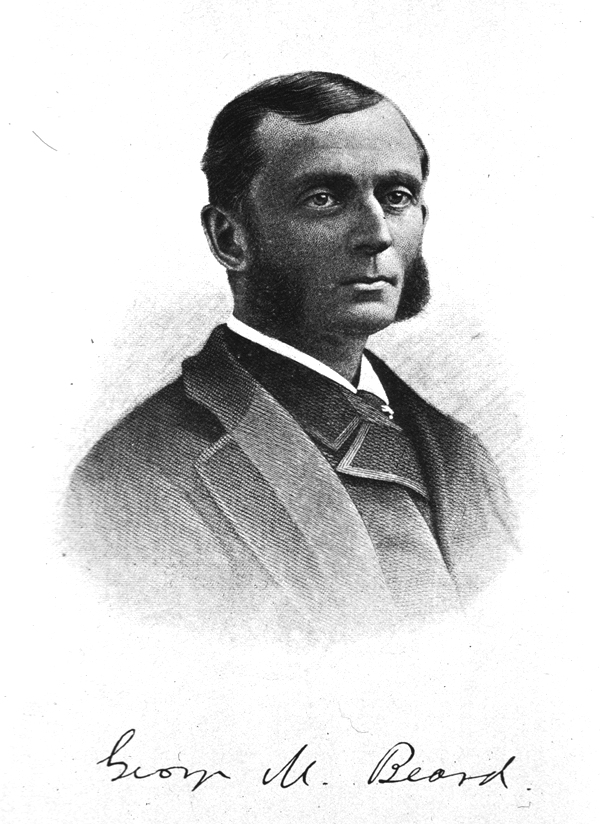
\includegraphics[scale=0.25]{../images/George_Miller_Beard.jpg}
\end{center}
 \caption{See page for author Public domain via Wikimedia Commons}
\label{fig: georgebeard}
\end{marginfigure}
 

Starting in the 1870s, Beard became increasingly interested in psychological disorders. In 1881, he published \emph{American Nervousness}, a book that came to define psychological treatment for a generation. `Nervousness' did not mean then what it means today: jitteriness or tension. Then, it denoted a kind of fundamental exhaustion—what we still call a `nervous breakdown'. Technically, Beard defined it as:

\begin{quote}

“deficiency of lack of nerve-force. This condition, together with all the symptoms of diseases that are evolved from it, has developed mainly within the nineteenth century, and is especially frequent and severe in the Northern and Eastern portions of the United States. Nervousness, in the sense here used, is to be distinguished rigidly and systematically from simple excess of emotion and from organic disease.” ~\citep[p. vi]{Beard:1881tg}
\end{quote}

It was caused by “modern civilization, which is distinguished from the ancient by these five characteristics: steam-power, the periodical press, the telegraph, the sciences, and the mental activity of women.” (p. vi)

Beard was building on both folk theory of innate energy as well as recent discoveries in neurology (compare, for example, the concurrent theory of `specific sense energies' proposed by Müller – see the \fullref{birthofpsychology:germanphysiologicalpsychologyinthe1880s-1890s.}.). But he extended his view to cover diseases such as “neurasthenia (nervous exhaustion{\ldots} hysteria, hay-fever, sick-headache, inebriety{\ldots} some and phases of insanity.” (p. vii) whose `signs' could include:

\begin{quote}

The nervous diathesis; susceptibility to stimulants and narcotics and various drugs, and consequent necessity of temperance; increase of the nervous diseases inebriety and neurasthenia (nervous exhaustion), hay-fever neuralgia, nervous dyspepsia, asthenopia and allied diseases and symptoms; early and rapid decay of teeth; premature baldness; sensitiveness to cold and heat; increase of diseases not exclusively nervous, as diabetes and certain forms of Bright's disease of the kidneys and chronic catarrhs; unprecedented beauty of American women; frequency of trance and muscle-reading; the strain of dentition, puberty and change of life; American oratory, humor speech and language; change in type of disease during the past half century, and the great intensity of animal life on this continent. (p. vii-ix)
\end{quote}

Beard died shortly after the publication of \emph{American Nervousness}, but his cause was taken up by Silas Wier Mitchell (1829--1914), who popularized a standard treatment for American Nervousness: the rest cure. As you can probably imagine, if the cause of American Nervousness was modern civilization, including women having a mental life, the cure was removal from modern civilization, including banning women from having a mental life.

In 1885, at the age of 25, Charlotte Perkins Gilman, a member of a prominent family of American progressives that included the abolitionist author Harriet Beecher Stowe, the suffragist Isabella Beecher Hooker, and the charismatic clergyman Henry Ward Beecher, gave birth to her only child Katharine Beecher Stetson. After the birth, Charlotte Perkins-Gilman experienced what we now recognize as a severe case of post-partum depression.

She was taken to see Silas Wier Mitchell. She described her experience of the treatment she received thus:

\begin{quote}

“During about the third year of this trouble I went, in devout faith and some faint stir of hope, to a noted specialist in nervous diseases, the best known in the country. This wise man put me to bed and applied the rest-cure, to which all still-good physique responded so promptly that he concluded there was nothing much the matter with me, and sent me home with solemn advice to `live as domestic a life as far as possible,' to `have but two hours' intellectual life a day' and `never touch a pen, brush or pencil again' as long as I lived. This was in 1887.” (“Why I wrote The Yellow Wallpaper, 1913)
\end{quote}

Her experiences you may know from the American Standard short story The Yellow Wallpaper (1892). Gilman acknowledged that she never suffered from the hallucinations her character does, but that she “came so near the borderline of mental ruin that I could see over.” (1913)
\begin{marginfigure}
 \begin{center}
     
\includegraphics[scale=0.25]{../images/The_Yellow_Wall_Paper}
\end{center}
 \caption{By Small, Maynard \& Company (File:The Yellow Wall Paper.djvu) (Public domain), via Wikimedia Commons}
\label{fig: yellowwallpaper}
\end{marginfigure}
 

While Beard and Wier Mitchell are today often ridiculed as snake-oil salesmen playing on political concerns over rapid modernization and the suffragist movement, they made a number of notable contributions to our commonsense understanding of psychological disorder. First, they indelibly linked mental disorders to neurology. As mentioned above, we still use phrases like `nervous breakdown' in common parlance to explain psychological disorder. Second, by proscribing puberty, birth, menopause and the `unprecedented beauty of American women' as prime causes of mental illness, they further established a link between the onset and frustration of sexuality with mental illness, a point upon which Freud would build psychoanalysis.

It would be a mistake, however, to accept the simplistic narrative that the doctors of this era were manipulating and abusing their female patients without their consent. Historians of Psychology Laura C. Ball and Jennifer L. Bazar have recently demonstrated that in some cases, some women aggressive sought out procedures, such as clitorectomies, in this period. In one remarkable case, a patient even `tormented the doctors to operate again.' ~\citep{Ball:2010tk}

One way to chart the rise of psychiatric diagnosis is to consider how people with mental illness are counted. Starting in 1830, the US census included categories for the disabled, including `blind' and `deaf.' ~\citep{Gorwitz:1974tt} From 1840--1870, the census included the category `idiocy\slash insanity.' Starting in 1880, however, the federal government began using categories of mental illness. In 1880, those categories were:
 \begin{longtable}[!t]{ |  p{1cm} |  p{1cm} |p{4.8cm} | }
\hline
21&\multicolumn{2}{ | p{5.8cm} | }{\tahead{Mental Disease, Insanity}} \\ \hline
      &00&Melancholy \\ \hline
     & 01&Mania \\ \hline
      &02&Hysteria \\ \hline
      &03&Nerves \\ \hline
      &04&Dementia \\ \hline
      &05&Insane (not elsewhere classified) \\ \hline
22&\multicolumn{2}{ | p{5.8cm} | }{\tahead{Mental Retardation, Idiocy}} \\ \hline
      &00&Idiotic \\ \hline

\caption{Mental Illness Classification used in the US Census of 1880}
\label{table: 1880classifications}
\end{longtable}


Readers of these sections will no doubt recognize this taxonomy as owing an intellectual debt to both Esquirol (Melancholy, Mania, Hysteria and Dementia) \emph{and} Beard (Nerves).

\subsubsection{Early Neurology --- Charcot}
\label{earlyneurology---charcot}

Charcot began his career at the Salpêtrière tending to the 'incurables'—the patients whose conditions had been classified as `idiocy' or `dementia.' Charcot saw himself primarily as a nosologist: a classifier or taxonomizer of disease, rather than a healer. His appointment was, in many ways, ideal. This was a patient population for which there was no hope of cure, and morever, had not been studied in a careful way. 

\begin{marginfigure}
 \begin{center}

     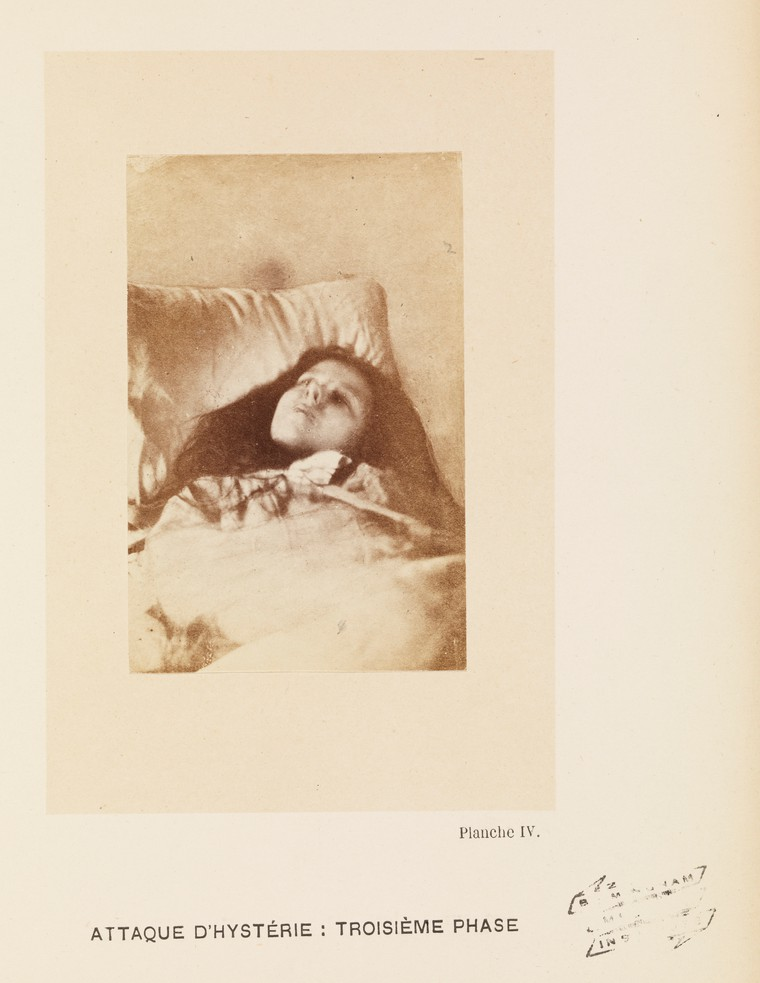
\includegraphics[scale=0.25]{../images/hysterie-troisiemephase.jpg}
\end{center}
 \caption{Photo of patient of M. Charcot in the Salpêtrière. From Wellcome images, https://wellcomecollection.org/works/fh922zk8 }
\label{fig: charcotpatient}
\end{marginfigure}


Charcot is, today, often classified as a neurologist. That is a bit of historicism, as there was no such field when he began work. In fact, the `neuron doctrine', or the idea that the nervous system is composed of individual cells called `neurons,' is not formally advanced until 1891. And it isn't until 1911 that Ramon y Cajal uses the Golgi stain to highlight neurons in the hippocampus, confirming the neuron doctrine.

None of that stopped Charcot from classifying a huge number conditions and diseases we still recognize today: multiple sclerosis, amyotrophic lateral sclerosis (ALS or “Lou Gerig's disease,” it was once called “Charcot's disease”), lenticulostriate artery (“Charcot's artery”), joint arthopathy (“Charcot's joint”), peroneal muscular atrophy (“Charcot-Marie-Tooth disease”), Charcot Wilbrand syndrome, Charcot's intermittent hepatic fever and even Parkinson's disease were all first named or described by Charcot.

Methodologically, Charcot advocated what he called the `anatomo-clinical' method, which meant careful anatomical analysis performed largely post-mortum combined with case studies of vivisection in both animals and human subjects. Once a behavioral deficiency has been identified, careful anatomical studies are carried out to determine any corresponding anatomical `deficiency,' or lesion. In his own words:

\begin{quote}

Allow me to recall to your minds the opinion which that most illustrious physiologist, Claude Bernard, thus expressed:—“Pathology,” said he, “should not he subordinated to physiology. Quite the reverse. Set up first the medical problem which arises from the observation of a malady, and afterwards seek for a physiological explanation. To act otherwise would be to risk overlooking the patient, and distorting the malady.” These are excellent words, which I have ventured to quote verbatim, because they are absolutely significant. They enable us to clearly understand that the whole domain of pathology appertains strictly to the physician, who alone can cultivate it and make it fruitful, and that it necessarily remains closed to the physiologist who, systematically confined within the precincts of his laboratory, disdains the teaching of the hospital ward. (p. 8)
\end{quote}

In 1878, he began extensive work on hypnosis. Hypnosis had been practiced at the Salpêtrière for over 50 years--since the days of Pinel, in fact. Charcot became increasingly interested in the therapeutic use of hypnosis to cure what he called `hysteria', a vaguely-defined collection of usually transient symptoms that included paralysis, anesthesias, visual or auditory agnosias, temporary blindness or deafness, amnesia and seizures. While `hysteria' came to be identified closely with women, Charcot himself believed that it could effect men, and treated many men that he diagnosed with hysteria.

This does not mean, however, that Charcot gave up his commitment to neurological explanations of behavior. He simply allowed functional and\slash or physiological explanations in addition to the anatomical. In his words:

\begin{quote}

There is another important fact in the history of neuroses in general, and of hysteria in particular, which clearly shows that these diseases do not form, in pathology, a class apart, governed by other physiological laws than the common ones. (13)
\end{quote}

I've quoted this passage because it is the first use of the word `neuroses' in print. It's root in neurological terminology is obvious, but here Charcot uses it to demarcate transient, psychological, functional or dynamic neurological conditions from the incurable, intransient, anatomical neurological conditions. The former we classify as ‘mental’, the latter ‘neurological’---even today. `Neurosis' thus supplants `mental alienation' and `nervousness' as the descriptor of the set of psychological conditions that cannot be explained physically, even though it’s root is connected to the idea of a physical manifestation in ‘neurons.’

In 1890, blocked by antisemitism in Germany from further education, a young Sigmund Freud came to study with M. Charcot. There, he learned the techniques of hypnosis and studied many cases of hysteria. Later in life, Freud frequently referred to Charcot as his `mentor,' and even attributed the idea that all neuroses originate `in the genitals' to Charcot.\footnote{In his `History of the Psychiatric Movement', Freud writes: “{\ldots}It was the case of the young married couple from the far East. The wife was a great sufferer and the husband was impotent, or exceedinly awkward. I head Charcot repeat: “Tâchez donc, je vous assure vous y arriverez.” Brouardel, who spoke less distinctly, must have expressed his astonishment that such symptoms as those of the young wife should have appeared as a result of such circumstances, for Charcot said suddenly and with great vivacity: “Mais, dans de cas pareils, c'est toujours la chose génital, toujours—toujours-toujours.” And while saying that, he crossed his hands in his lap an jumped up and down several times, with the vivacity peculiar to him.” ~\citep[p. 937--938]{Freud:1938vi}

We know that George Beard and Silas Wier Mitchell had the same view at this point, and that Freud was familiar with their work on ‘hysteria.’ What is unknown, given that Freud's retelling of this anecdote is based on his memory alone, is the accuracy of this story. It might be the case, and it might just be Freud misattributing a theory he picked up from Beard and Wier Mitchell to his mentor years after the fact.}

In his eulogy for Charcot, Sigmund Freud said:

\begin{quote}

He was not a reflective man, not a thinker: He had the nature of an artist—he was, as he himself said, a `visuel', a man who sees{\ldots} He used to look again and again at the things he did not understand, to deepen his impression of them day by day, till suddenly an understanding of them dawned on him. In his mind's eye the apparent chaos presented by the continual repetition of the same symptoms then ave way to order: the new nosological picture emerged, characterized by the constant combination of certain groups of symptoms{\ldots} He might be heard to say that the greatest satisfaction a man could have was to see something new-- that is, to recognize it as new; and he remarked against and again n the difficulty and value of this kind of `seeing'. (Quoted in Mad, Bad and Sad, p. 128)
\end{quote}

It should be fairly obvious that Freud here is dismissing, essentially, Charcot's Baconian approach to scientific classification: careful, close observation with only careful, conservative theoretical suppositions. Unlike Charcot, who is remembered only in the names of the diseases he classified, Freud became globally famous for his theoretical suppositions. Whereas Charcot was content with describing neuroses and localizing them in the nervous system, Freud sought to explain the origins of neuroses in non-physical terms.

\subsection{Rise of Psychoanalysis}
\label{riseofpsychoanalysis}

\subsubsection{Hysteria and Hypnosis: Freud \& Breuer on Anna O.}
\label{hysteriaandhypnosis:freudbreueronannao.}

By the end of the 19th century, we are beginning to find general agreement that mental illnesses are characterized by symptoms with no bodily, physical (or in Beard's terms `organic') explanation.\footnote{See, for example, Drellich, Marvin G. “Classical Psychoanalytic School” in ~\citep{Arieti:1974tm}} That understanding defined the limits of psychiatry. When a condition could be explained in anatomical terms, it was no longer considered psychiatric and reverted to medical or neurological. When it could not be understood physically---when it had to be explained in terms of 'psychic energy---it was given to the psychiatrists.

This thesis was not challenged largely because psychiatrists practiced in hospitals that contained psychiatric patients. That sounds circular, but it isn't: Pinel, Esquirol and Charcot were attempting to create a theory of mental illness that could explain the patients they saw before them. The patients they saw before them were not brought there because they fit the theory, or because they had chosen to be there. They were brought to the Bicêtre and Salpêtrière when the rest of the medical community had given up attempting to explain their symptoms.

The same can be said for Beard and Wier Mitchell: Perkins Gilman was taken to see Wier Mitchell only after all physical interventions had failed.

These founders of psychiatry theorized about a population that had been deemed mentally ill \emph{because the medical community had given up explaining their symptoms}. Not the other way around. The Psychiatric hospital was a kind of catch-all for those individuals whose symptoms could not be alleviated by physical medicine, and hence it is unsurprising that the definitions of insanity we find in this era require the absence of a physical explanation.

Without a control population, there was no way these classifications could tease apart underlying conditions from any effects that may have resulted from being classified this way in the first place. 

In 1880, Josef Breuer, a student of the great psycho-physiologist Ewald Hering, was studying the ear as a part of his research at Vienna General Hospital. It was there that he first met `Anna O.', a young woman with an extremely acute cough. Finding \textbf{no physical reason} for the cough, her family physician diagnosed her with “typical \emph{tussis nurvosa} [nervous cough]” ~\citep[p 27]{Freud:kVwxqGOZ} 

Shortly thereafter a number of other symptoms arose. Freud \& Breuer describe her case thusly:

\begin{quote}

Before this time she too had always enjoyed good health, showing no sign of nervous indisposition during her development. Of considerable intelligence, remarkably acute powers of reasoning, and a clear-sighted intuitive sense, her powerful mind could have digested, needed even, more substantial intellectual nourishment, but failed to receive it once she had left school. Her rich poetic and imaginative gifts were controlled by a very sharp and critical common sense. The latter also made her quite closed to suggestion. Only arguments had any influence on her, assertions were without effect. Her will was energetic, tenacious and persistent, sometimes heightened to such obstinacy that it would give way only out of kindness and consideration for others.

One of her principle traits was a sympathetic kindness. Even during her illness, she benefited greatly from the care and support she gave to some sick and poor people, for it allowed her to satisfy a strong drive. Her spirits always tended slightly to exaggeration, whether of joyfulness or grief, and as a consequence she was also somewhat moody. The element of sexuality was remarkably undeveloped: the patient, whose life became transparent to me in a way that seldom happens between people, had never been in love, and not once in the mass of hallucinations that occurred during her illness did this element of the inner life emerge{\ldots}

{\ldots}The course of the illness falls into several distinct phases. They are as follows:

A) Latent incubation. From mid-July 1880 to approximately 10 December. This case was exceptional because it afforded so complete an insight into a phase that in most cases escapes us, and for this reason alone its pathological interest could not be overestimated. I will expound on this part of the history later.

B) Manifest illness: a peculiar kind of psychosis, paraphasia, \emph{stabismus convergens} [convergent squint], sever visual disturbance, paralyzing contractures, complete paralysis in the upper right and both lower extremities, partial paralysis in the upper left extremity, paresis of the neck muscles. A gradual reduction in the contracture of the right extremities. Some improvement, interrupted by a sever psychical trauma (death of the father) in April, after which

C) A period of continual somnambulism ensues, which then alternates with more normal states; continuation of a series of chronic symptoms until December 1881.

D) Gradual winding down of mental states and symptoms until June 1882. ~\citep[p25--26]{Freud:kVwxqGOZ}
\end{quote}

Breuer took over her care during the period of `manifest illness,' during which, Anna O. slept for great periods of time (`somnambulism'), but when she awoke in the evening, she would complain of `torment.' Her speech lost all grammatical structure (`paraphasia') and she would piece together words and phrases from the five distinct languages she spoke, producing an incomprehensible jargon. This same jargon appeared in writing, so Breuer knew that it was not a disfunction of the physical mechanism of speech.

In the early spring of 1881, Anna O fell mute for a period of two weeks. At this point, Breuer claims that he 

\begin{quote}

“knew she had taken great offense at something and had resolved to say nothing about it. When I guessed as much and forced her to talk about it, the inhibition, which had until then made it impossible for her to speak about anything else either, disappeared.” ~\citep[p 29]{Freud:kVwxqGOZ}
\end{quote}

After her father's death, her illness became much more severe. Breuer noticed, however, that her periods of sleep in the later afternoon, during which she was `tormented' by hallucinations, resembled hypnotic states. He decided to preemptively hypnotize her and prompt her to `talk through' these tormenting phantasies. The symptoms subsided quickly. The day after a session, she would become `quite calm' and `agreeable, obedient, industrious and even in good spirits'. The second day after a session she would be `increasingly moody, contrary and disagreeable, and this worsened on the third.' Anna O. named these sessions (in English) the `talking cure' and `chimney-sweeping.' Breuer preferred the more sophisticated `cathartic procedure.'

Breuer communicated this to his friend Sigmund Freud, who offered to co-author a paper laying out the findings. That paper, titled `The Psychic Mechanism of Hysterical Phenomena,' first appeared in 1893, but was republished as the first chapter of Freud and Breuer's \emph{Studies on Hysteria} ~\citep[1895]{Freud:kVwxqGOZ}. In it, Freud and Breuer propose a new form of hysteria, called `traumatic hysteria', which they conjecture is always connected to some traumatic event that evokes the syndrome. They further hypothesize that the traumatic event can be unavailable to the conscious, reflective mind of patient---i.e. be unconscious---yet still be causally responsible for the hysterical symptoms. Moreover, they hypothesize that making the patient aware of the trauma, via Breuer’s `cathartic procedure' using hypnosis if necessary, alleviates the hysteria.

\subsubsection{Freud: The foundation of psychoanalysis}
\label{freud:thefoundationofpsychoanalysis}

The seeds of psychoanalysis were planted by Charcot and Breuer, but they did not develop into a full-fledged system of Psychiatry until Freud worked independently. Building on his theory of unconscious trauma to explain hysteria, Freud hypothesizes that traumatic events may manifest themselves in the mind indirectly in the form of symbols. He then went on to realize that the fantasy lives of the psychotic are full of such symbols, and recovering the original trauma requires investigation of the mechanisms of symbolization.

It was this realization that gives us the basis for psychoanalysis, for it is this realization that allows Freud to argue that the hallucinations and fantasies experiences by the psychotic are not significantly different from the dreams of the sane. Whereas prior to Freud, dreams and hallucinations were thought to be without meaning, after Freud they were seen as full of symbolic representations, the meanings of which were available empirically through systematic investigation of the mechanisms of psychological representation. Freud's proposed mechanisms are introduced in the \ref{classical} section on page \pageref{classical} of the game book.

The barrier between the mentally ill and the mentally healthy had been permanently broken.\footnote{I am simplifying here a bit. While Freud is commonly believed to originate the idea that dreams and psychotic hallucinations were best understood on a continuum, the ideas appears in the work of the British associationist Alexander Bain. See, e.g. ~\citep[p. 45]{Bain:1903tf}} No longer does the theory of psychiatry apply only to those who cannot be helped by medicine. Now the theory applies to everyone: a healthy person could become ill through unhealthy habits of mental representation, and ill people could become healthy through the process of discovering their habits of mental representation and recognizing their unconscious traumas. 

This conflation of psychiatric conditions and normal life left Freud in the precarious position of having to define `mental illness.' He did so thus:
\begin{apatextbox}{Freud’s Definition of Mental Illness} Symptoms—and of course we are dealing now with psychical (or psychogenic) symptoms and psychical illness—are acts detrimental, or at least useless, to the subject's life as a whole, often complained by him as unwelcome and bringing unpleasure or suffering to him. ~\citep[p. 445]{Freud:QdOvAgyZ}

\label{def:freud}\end{apatextbox}

\textbf{Neurosis v. Psychosis.} One of the hallmarks of Freud's theory is his thesis that the there is no hard and fast distinction to be made between the mentally ill and the mentally healthy. His \emph{Introductory Lectures} are structured to introduce the reader to psychopathology in everyday life before extending the analysis of common activities to psychotics and neurotic patients. As such, there are no hard and fast definitions of psychosis and neurosis\footnote{The distinction between neurosis and psychosis has always been controversial. Consider Pavlov's comment in his 1927 lectures: “Contemporary medicine distinguishes ``nervous'' and ``psychic'' disturbances-neuroses and psychoses, but this distinction is, of course, only arbitrary. No real line of demarcation can be drawn between these two groups: it is impossible to imagine a deviation of higher activities from normal without a functional or structural disturbance of the cortex.” ~\citep[Lecture 23]{Pavlov:1946ws}}.

During the course of normal development of mentally healthy adults, the ego must become `reasonable': it must no longer let “itself be governed by the pleasure principle, but obeys the reality principle, which also at bottom seeks to obtain pleasure, but pleasure which is assured through taking account of reality, even though it is pleasure postponed and diminished.” (p. 444) A neurotic's ego fails to make this transition, and gets stuck at one point in development. Thus, the neurotic's libido and ego are still struggling in a child-like way, but the contents of the struggle have been transformed into objects of adulthood. Neurotic symptoms are the “outcome of a conflict which arises over a new method of satisfying the libido” (p. 446) and a person is ill from neurosis only if “his ego has lost the capacity to allocate his libido in some way” (p. 480). A psychotic patient, however, has lost the battle for the reality principle, and the libido has created its own reality.

The object of a neurosis, then, is relevant to the diagnosis only insofar as it is a stand-in for the actual conflict by the mechanisms of repression, reaction formation, isolation, etc. According to Freud: “clinical psychiatry takes little notice of the outward form or content of individual symptoms, but psychoanalysis takes matters up at precisely that point and has established in the first place the fact that symptoms have a sense and are related to the patient's experience.” (p. 318)

See Lectures 22 and 23 of the \emph{Introductory Lectures} for a full discussion of neurosis and its origins.

\subsubsection{The Clark Lectures}
\label{theclarklectures}

In 1909, G. Stanley Hall, first president of the American Psychological Association, invited Freud and Jung to give a series of lectures at Clark University. The conference itself was a major moment in the intellectual history of America, as such luminaries as William James, Franz Boas, Adolf Meyer and E.B. Tichner were in attendance, as well as the famed Anarchist Emma Goldman.\footnote{See, for example ~\citep{Jacoby:2009tt}

Experienced Reactors may recognize Emma Goldman from Mary Jane Tracey's Suffrageist game}

After the lectures, James Jackson Putnam, a neurologist in New York City, invited Freud and Jung to retire to his family's Adirondack `great camp' for the weekend. (~\citep{Prochnik:FiwLnN1z}) Putnam became an important advocate for psychoanalysis in the United States, establishing its legitimacy as a treatment for hysteria. While there are articles prior to 1909 on psychoanalysis (notably one by Putnam himself in 1906), we don't find significant discussion of psychoanalysis in the mainstream journals of Psychology until after the Clark lectures.\footnote{For a discussion, see ~\citep{Hornstein:2002wq}} An effort to convince the American public of the scientific nature of psychoanalysis was mounted by Putnam camp attendees A.A. Brill, founder of the New York Psychoanalytic Society, and Ernest Jones, student of Freud. By 1916, Jones had published 20 articles, notes and reviews in the Journal of Abnormal Psychology offering or advocating for psychoanalysis.\footnote{See, e..g. ~\citep[p. 474]{Hornstein:2002wq}}

Putnam and Freud went on to become close friends, and Putnam spent much of the rest of his career attempting to professionalize and regularize the practice of psychiatry. He founded the American Psychoanalytic Association (APsaA) in 1911, which is still active today. His posthumously published \emph{Addresses on Psychoanalysis}, which contains a preface by Freud himself, not only seeks to introduce Freudian theory to his scientific community, but also to dispel misunderstanding gained “through the gossip of prejudice and misconception” ~\citep[p. 3]{Putnam:1921uc}.

Putnam’s influence here cannot be understated. Putnam introduced psychoanalytic ideas to the budding field of medical neurology. His position as a medical doctor at Harvard gave psychoanalysis legitimacy as a medical practice in America, and his stature in the neurological community helped to assuage any doubts about the lack of a physical basis for the hypothetical entities posited by Freud's structural hypothesis.

The story is not all smooth sailing. In 1916, the Princeton philosopher and psychologist Warren Fite reviewed of Jung's \emph{Psychology of the Unconscious} for \emph{The Nation}, writing that it “presents some five hundred-odd pages of incoherence and obscenity in the form of a psycho-analytic interpretation of the experiences of a sentimental young American woman.” ~\citep{Fite:1916tk} The fact that the United States was at war with Germany didn't help the psychoanalytic cause: Christine Ladd-Franklin, a student of C.S. Peirce and protege of no less than Hermann Helmholtz as well as one of the first women in the APA, called Freud's theory the product of an “undeveloped{\ldots} German mind.”

What followed is a history of tension between those in the psychological and psychoanalytic communities. Helped by the military's preference for psychoanalysts in the treatment of `shell-shock' during WWI and `combat fatigue' in WWII, psychoanalysis gained credibility in the eyes of the American public.\footnote{See Chapter 1 of ~\citep{Menninger:3tUbEPj8} for an interesting discussion of this history.}

\subsection{Classification of Mental Illness, 1918--1952}
\label{classificationofmentalillness1918-1952}

In 1917 during its annual meeting in New York, the American Medico-Psychological Association (now the American Psychiatric Association) in cooperation with the National Commission on Mental Hygiene formed a committee on statistics and charged it with creating a guide for classifying mental illness. The resulting document, \emph{Statistical Manual for the Use of Institutions for the Insane}, was published in 1918 and adopted around the nation. It is available freely on google books. The manual outlined 21 medical-psychological categories, displayed in table \ref{table: 1918Classification}:

 \begin{longtable}[!t]{ | p{4cm} | p{10.8cm} | }
\hline
\tahead{Major Category}&\tahead{Minor Category} \\ \hline
\multicolumn{2}{ | p {14.8cm} | }{1. Traumatic psychoses} \\ \hline
 &(a) Traumatic delirium \newline
(b) Traumatic constitutional \newline
(c) Post-traumatic mental enfeeblement (dementia)\\

\multicolumn{2}{ | p {14.8cm} | }{2. Senile psychoses} \\ \hline
 &(a) simple deterioration\newline
(b) Presbyophrenic type\newline
(c) Delirious and confused types\newline
(d) Depressed and agitated states in addition to deterioration\newline
(e) Paranoid types\newline
(f) Pre-senile types \\ \hline

\multicolumn{2}{ | p {14.8cm} | }{3. Psychoses with cerebral arteriosclerosis} \\ \hline
\multicolumn{2}{ | p {14.8cm} | }{4. General paralysis} \\ \hline
\multicolumn{2}{ | p {14.8cm} | }{5. Psychoses with cerebral syphilis} \\ \hline
\multicolumn{2}{ | p {14.8cm} | }{6. Psychoses with Huntington's chorea} \\ \hline
\multicolumn{2}{ | p {14.8cm} | }{7. Psychoses with brain tumor} \\ \hline
\multicolumn{2}{ | p {14.8cm} | }{8. Psychoses with other brain or nervous diseases} \\ \hline
 & The following are the more frequent affections and should be specified in the diagnosis\newline
     Cerebral embolism\newline
     Paralysis agitans\newline
     Meningitis, tubercular or other forms\newline
        (to be specified)\newline
     Multiple sclerosis\newline
     Tabes\newline
     Acute chorea\newline
     Other conditions (to be specified) \\ \hline
\multicolumn{2}{ | p {14.8cm} | }{9. Alcoholic psychoses} \\ \hline
 &(a) Pathological intoxication\newline
(b) Delirium tremens\newline
(c) Korsakow's psychosis\newline
(d) Acute hallucinosis\newline
(e) Chronic hallucinosis\newline
(f) Acute paranoid type\newline
(g) Chronic paranoid type\newline
(h) Alcoholic deterioration\newline
(i) Other types, acute or chronic \\ \hline

\multicolumn{2}{ | p {14.8cm} | }{10. Psychoses due to drugs or other exogenous toxins} \\ \hline
 &(a) Opium (and derivatives), cocaine, bromides, chloral, etc. alone or combined (to be specified)\newline
(b) Metals, as lead, arsenic, etc. (to be specified)\newline
(c) Gases (to be specified)\newline
(d) Other exogenous toxins (to be specified) \\ \hline
\multicolumn{2}{ | p {14.8cm} | }{11. Psychoses with pellagra}  \\ \hline
\multicolumn{2}{ | p {14.8cm} | }{12. Psychoses with other somatic diseases} \\ \hline
 &(a) Delirium with infectious diseases\newline
(b) Post-infectious psychosis\newline
(c) Exhaustion-delirium\newline
(d) Delirium of unknown origin\newline
(e) Cardio-renal diseases\newline
(f) Disease of the ductless glands\newline
(g) Other diseases or conditions (to be specified) \\ \hline
\multicolumn{2}{ | p {14.8cm} | }{13. Manic-depressive psychoses} \\ \hline
 &(a) Manic type \newline
(b) Depressive type \newline
(c) Stupor \newline
(d) Mixed type \newline
(e) Circular type \\ \hline
\multicolumn{2}{ | p {14.8cm} | }{14. Involution melancholia} \\ \hline
\multicolumn{2}{ | p {14.8cm} | }{15. Dementia praecox} \\ \hline
 & (a) Paranoid type \newline
(b) Catatonic type \newline
(c) Hebephrenic type \newline
(d) Simple type \\ \hline
\multicolumn{2}{ | p {14.8cm} | }{16. Paranoia or paranoic conditions} \\ \hline
\multicolumn{2}{ | p {14.8cm} | }{17. Epileptic psychoses} \\ \hline
 &(a) Deterioration \newline
(b) Clouded states \newline
(c) Other conditions (to be specified) \\ \hline
\multicolumn{2}{ | p {14.8cm} | }{18. Psychoneuroses and neuroses} \\ \hline
 &(a) Hysterical type \newline
(b) Psychasthenic type \newline
(c) Neurasthenic type \newline
(d) Anxiety neuroses \\ \hline
\multicolumn{2}{ | p {14.8cm} | }{19. Psychoses with constitutional psychopathic inferiority}  \\ \hline
\multicolumn{2}{ | p {14.8cm} | }{20. Psychoses with mental deficiency} \\ \hline
\multicolumn{2}{ | p {14.8cm} | }{21. Undiagnosed psychoses} \\ \hline
\multicolumn{2}{ | p {14.8cm} | }{22. Not insane} \\ \hline
 & (a) Epilepsy without psychosis \newline
(b) Alcoholism with psychosis \newline
(c) Drug addition without psychosis \newline
(d) Constitutional psychopathic inferiority without psychosis \newline
(e) Mental deficiency without psychosis \newline
(f) Others (to be specified)\\ \hline
\caption{\emph{Statistical Manual for the Use of Institutions for the Insane classification of insanity}, 1918}
\label{table: 1918Classification}
\end{longtable}


In 1928, the New York Academy of Medicine invited the Public Health Service, the Army and Navy Medical Departments and the American Hospital Association to collaborate on a standard nomenclature of disease. That standard was first published in 1933 as \emph{A Standard Classified Nomenclature of Disease}, generally referred to as \emph{The Standard}, and was widely used until at least the 1960s. ~\citep{Houts:2000vp}

In its original form, it used the following ten categories, as displayed in table \ref{table: 1933Classification}:

 \begin{longtable}[!t]{ | p{13.8cm}  | }
\hline
0 Diseases due to prenatal influences\\
1 Diseases due to lower plant and animal parasites\\
2 Diseases due to higher plant and animal parasites\\
3 Diseases due to intoxication\\
4 Diseases due to trauma or physical agents\\
5.0 Diseases due to circulatory disturbances\\
5.5 Diseases due to disturbances of innervation or of psychic control\\
6 Diseases due to or consisting of static mechanical abnormality (obstruction; calculus; displacement and gross changes in form etc., due to unknown cause).\\
7 Diseases due to disorders of metabolism, growth or nutrition\\
8 New growths\\
9 Diseases due to unknown or uncertain causes, the structural reaction (generative, infiltrative, inflammatory, proliferate, sclerotic, or reparative) to which is manifest; and hereditary and familial diseases of this nature.\\
X Diseases due to unknown or uncertain causes, the functional reaction to which is alone manifest; and hereditary and familial diseases of this nature.\\ \hline
\caption{\emph{Standard Classified Nomenclature classification of disease}, 1933}
\label{table: 1933Classification}
\end{longtable}


You may notice that the medical classification is entirely based on the origin or cause of a condition ('Diseases \textbf{due to{\ldots}}’), not the symptoms. In the \ref{table: 1918Classification}, classification system, mental diseases are classified by the Freudian terms `psychosis' and `neurosis', except for melancholy and dimentia.

During WWII, psychiatrists classified patients according to the standards of the branch of the armed forces for which they worked. In 1943, Brigadier General William C. Menninger issued a bulletin called “Medical 203” that laid the foundations for medical classification of mental illness. The Navy, Army and Veterans affairs branches all used slightly different diagnostic criteria and classifications.

The International Statistical Classification of Diseases (ICD) included a taxonomy of mental disorders for the first time in 1949. Its classification system is displayed in table \ref{table: 1949Classification}:

 \begin{longtable}[!t]{ | p{2cm} | p{11.8cm} | }
\hline

\tahead{(300-309)}&\tahead{Psychoses} \\ \hline
300&Schizophrenic disorders (dementia praecox) \\
300.0&     Simple type\\
300.1&     Hebephrenic type\\
300.2&     Catatonic type\\
300.3&     Paranoid type\\
300.4&     Acute schizophrenic reaction\\
300.5&     Latent schizophrenia\\
300.6&     Schizo-affective psychosis\\
300.7&     Other and unspecified\\
301&Manic-depressive reaction\\
301.0&     Manic and circular\\
301.1&     Depressive\\
301.2&     Other\\
302&Involutional melancholia\\
303&Paranoia and paranoid states\\
304&Senile psychosis\\
305&Presenile psychosis\\
306&Psychosis with cerebral arteriosclerosis\\
307&Alcoholic psychosis\\
308&Psychosis of other demonstrable aetiology\\
308.0&     Resulting from brain tumour\\
308.1&     Resulting from epilepsy and other convulsive disorders\\
308.2&     Other\\
309&Other and unspecified psychoses\\ \hline
\tahead{(310-318)}&\tahead{Psychoneurotic disorders} \\ \hline
310&Anxiety reaction without mention of somatic symptoms\\
311&Hysterical reaction without mention of anxiety reaction\\
312&Phobic reaction\\
313&Obsessive-compulsive reaction\\
314&Neurotic-depressive reaction\\
315&Psychoneurosis with somatic symptoms (somatisation reaction) affecting circulatory system\\
315.0&     Neurocirculatory asthenia\\
315.1&     Other heart manifestations specified as of psychogenic origin\\
315.2&     Other circulatory manifestations of psychogenic origin\\
316&Psychoneurosis with somatic symptoms (somatisation reaction) affecting digestive system\\
316.0&     Mucous colitis specified as of psychogenic origin\\
316.1&     Irritability of colon specified as of psychogenic origin\\
316.2&     Gastric neuroses\\
316.3&     Other digestive manifestations specified as of psychogenic origin\\
317&Psychoneurosis with somatic symptoms (somatisation reaction) affecting other systems\\
317.0&     Psychogenic reactions affecting respiratory system\\
317.1&     Psychogenic reactions affecting genito-urinary system\\
317.2&     Pruritus of psychogenic origin\\
317.3&     Other cutaneous neuroses\\
317.4&     Psychogenic reactions affecting musculoskeletal system\\
317.5&     Psychogenic reactions affecting other systems\\
318&Psychoneurotic disorders, other, mixed and unspecified types\\
318.0&     Hypochondriacal reaction\\
318.1&     Depersonalisation\\
318.2&     Occupational neurosis\\
318.3&     Asthenic reaction\\
318.4&     Mixed\\
318.5&     Of other and unspecified types\\ \hline
\tahead{(320-326)}&\tahead{Disorders of character, behaviour, and intelligence}\\ \hline
320&Pathological personality\\
320.0&     Schizoid personality\\
320.1&     Paranoid personality\\
320.2&     Cyclothymic personality\\
320.3&     Inadequate personality\\
320.4&     Antisocial personality\\
320.5&     Asocial personality\\
320.6&     Sexual deviation\\
320.7&     Other and unspecified\\
321&Immature personality\\
321.0&     Emotional instability\\
321.1&     Passive dependency\\
321.2&     Aggressiveness\\
321.3&     Enuresis characterising immature personality\\
321.4&     Other symptomatic habits except speech impediments\\
321.5&     Other and unspecified\\
322&Alcoholism\\
322.0&     Acute\\
322.1&     Chronic\\
322.2&     Unspecified\\
323&Other drug addiction\\
324&Primary childhood behaviour disorders\\
325&Mental deficiency\\
325.0&     Idiocy\\
325.1&     Imbecility\\
325.2&     Moron\\
325.3&     Borderline intelligence\\
325.4&     Mongolism\\
325.5&     Other and unspecified types\\
326&Other and unspecified character, behaviour and intelligence disorders\\
326.0&     Specific learning defects\\
326.1&     Stammering and stuttering of non-organic origin\\
326.2&     Other speech impediments of non-organic origin\\
326.3&     Acute situational maladjustment\\
326.4&     Other and unspecified\\ \hline
\caption{\emph{ICD-6 classification of mental diseases}, 1949}
\label{table: 1949Classification}
\end{longtable}

In the interest of unifying these different classification schema, the American Psychiatric Association voted to create the first Diagnostic and Statistical Manual (DSM). The nomenclature committee adapted the Medical 203 bulletin into the DSM and circulated it to a randomly selected sample of the membership (10\%). When it was overwhelmingly approved by those who replied, the APA adopted it as the standard for diagnosis in medical treatment of psychological disorders. It is included as Appendix \ref{app: DSMI}
The first DSM distinguished between “Disorders caused by or associated with impairment of brain tissue function,” “Mental Deficiency,” “Disorders of psychogenic origin or without clearly defined physical cause or structural change in the brain” and “Nondiagnostic Terms for Hospital Record.” This fourth category included “Alcoholic intoxication (simple drunkenness),” and “Dead on admission.” It is the third category, those without a physical cause, that is of the most interest to us. They are displayed here in table \ref{table: 1952Classification} 

 \begin{longtable}[!t]{ | p{2cm} | p{8.8cm} | p{2cm} | }
\hline
\multicolumn{2}{ | p{12.8cm} | }{\tahead{Psychotic Disorders}}& \tahead{ICD-6 Ref} \\ \hline
--7&\multicolumn{2}{ | p{12.8cm} | }{Disorders due to disturbance of metabolism, growth, nutrition or endocrine function} \\
000-796&Involuntary psychotic reaction&(302) \\ \hline
--x&\multicolumn{2}{ | p{12.8cm} | }{Disorders of psychogenic origin or without clearly defined tangible cause or structural change} \\ \hline
000-x10&Affective reactions&(301.2) \\
     000-x11&     Manic depressive reaction, manic type&(301.0) \\
     000-x12&     Manic depressive reaction, depressive type&(301.1) \\
     000-x13&     Manic depressive reaction, other&(301.2) \\
     000-x14&     Psychotic depressive reaction&(309.0)* \\
000-x20&Schizophrenic reactions&(300.7)* \\
     000-x21&     Schizophrenic reaction, simple type&(300.0) \\
     000-x22&     Schizophrenic reaction, hebephrenic type&(300.1) \\
     000-x23&     Schizophrenic reaction, catatonic type&(300.2) \\
     000-x24&     Schizophrenic reaction, paranoid type&(300.3) \\
     000-x25&     Schizophrenic reaction, acute undifferentiated type&(300.4) \\
     000-x26&     Schizophrenic reaction, chronic undifferentiated type&(300.7) \\
     000-x27&     Schizophrenic reaction, schizo-affective type&(300.6) \\
     000-x28&     Schizophrenic reaction, childhood type&(300.8) \\
     000-x29&     Schizophrenic reaction, residual type&(300.5) \\
000-x30&Paranoid reactions&(303) \\
     000-x31&     Paranoia&(303) \\
     000-x32&     Paranoid state&(303) \\
000-xy0&Psychotic reaction without clearly defined structural change, other than above&(309.1)* \\ \hline
\multicolumn{3}{ | p{13.8cm} | }{\tahead{Psychophysiologic autonomic and visceral disorders}} \\ \hline
--55&\multicolumn{2}{ | p{12.8cm} | }{Disorders due to disturbance of innervation or of psychic control} \\ \hline
001-580&Psychophysiologic skin reaction&(317.3) \\
002-580&Psychophysiologic musculoskeletal reaction&(317.4) \\
003-580&Psychophysiologic respiratory reaction&(317.0) \\
004-580&Psychophysiologic cardiovascular reaction&(315.2) \\
005-580&Psychophysiologic hemic and lympathic reaction&(317.5) \\
006-580&Psychophysiologic gastrointestinal reaction&(316.3) \\
007-580&Psychophysiologic genito-urinary reaction&(317.1) \\
008-580&Psychophysiologic endocrine reaction&(317.5) \\
009-580&Psychophysiologic nervous system reaction&(318.3) \\
00x-580&Psychophysiologic reaction of organs of special sense&(317.5) \\ \hline
\multicolumn{3}{ | p{13.8cm} | }{\tahead{Psychoneurotic Disorders}} \\ \hline
--x&\multicolumn{2}{ | p{12.8cm} | }{Disorders of psychogenic origin or without clearly defined tangible cause of structural change} \\ \hline
000-x00&Psychoneurotic reactions&(318.5)* \\
     000-x01&     Anxiety reaction&(310) \\
     000-x02&     Dissociative reaction&(311) \\
     000-x03&     Conversion reaction&(311) \\
     000-x04&     Phobic reaction&(312) \\
     000-x05&     Obsessive compulsive reaction&(313) \\
     000-x06&     Depressive reaction&(314) \\
     000-x0y&     Psychoneurotic reaction, other&(318.5*) \\ \hline
\multicolumn{3}{ | p{13.8cm} | }{\tahead{Personality Disorders}} \\ \hline
--x&\multicolumn{2}{ | p{12.8cm} | }{Disorders of psychogenic origin or without clearly defined tangible cause of structural change} \\ \hline
000-x40&Personality pattern disturbance&(320.7) \\
     000-x41&     Inadequate personality&(320.3) \\
     000-x42&     Schizoid personality&(320.0) \\
     000-x43&     Cyclothymic personality&(320.2) \\
     000-x44&     Paranoid personality&(320.1) \\
000-x50&Personality trait disturbance&(321.5) \\
     000-x51&     Emotionally unstable personality&(321.0) \\
     000-x52&     Passive-aggressive personality&(321.1) \\
     000-x53&     Compulsive personality&(321.5) \\
     000-x54&     Personality trait disturbance, other&(321.5)* \\
000-x60&Sociopathic personality disturbance&(320.7)* \\
     000-x61&     Antisocial reaction&(320.4) \\
     000-x62&     Dyssocial reaction&(320.5) \\
     000-x63&     Sexual deviation. Specify supplementary term&(320.6) \\
     000-x64&     Addiction& \\
         000-x641&          Alcoholism&(322.1) \\
         000-x642&          Drug addiction&(323) \\
000-x70&Special symptom reactions&(321.4)* \\
     000-x71&     Learning disturbance&(326.0)* \\
     000-x72&     Speech disturbance&(326.2)* \\
     000-x73&     Enuresis&(321.3) \\
     000-x74&     Somnambulism&(321.4) \\
     000-x7y&     Other&(321.4)* \\ \hline
\multicolumn{3}{ | p{13.8cm} | }{\tahead{Transient Situational Personality Disorders}} \\ \hline
000-x80&Transient situational personality disturbance&(326.4)* \\
     000-x81&     Gross stress reaction&(326.3)* \\
     000-x82&     Adult situational reaction&(326.6)* \\
     000-x83&     Adjustment reaction of infancy&(324.0)* \\
     000-x84&     Adjustment reaction of childhood&(324.1)* \\
         000-x841&          Habit disturbance&(324.1)* \\
         000-x842&          Conduct disturbance&(324.1)* \\
         000-x843&          Neurotic disturbance&(324.1)* \\
     000-x85&     Adjustment reaction of adolescence&(324.2)* \\
     000-x86&     Adjustment reaction of late life&(326.5)* \\ \hline
\caption{\emph{DSM-I Classification of mental disorders} Corresponding diagnosis from the ICD-6 are noted in the right most column, 1952}
\label{table: 1952Classification}
\end{longtable}


Notice that while the major classification here is `Psychotic Disorders', the word ``reaction'' appears in 41 of the 48 diagnoses. See the overview of Classical Psychanalysis in section \ref{classical} on page \pageref{classical}.

The APA published the revised DSM-II in 1968. It is included as Appendix \ref{app: DSMII}..

\subsection{The Rise of Psychopharmacology}
\label{theriseofpsychopharmacology}

Because psychoanalysis tended to be confined to clinical, military settings in the US, a kind of stable truce—the more cynical might even say a 'cold war’---settled over the conflict between behaviorism and psychoanalysis. By and large, psychoanalysis confined itself to the medical setting; while behaviorism confined itself to pure research. There were, no doubt, volleys across the bow of one or the other from time to time. But until Skinner's wide-ranging proposals for behaviorism as social reformation, there were few open hostilities.

Much of the scientific credibility for psychoanalysis turned on its success in treating psychotic patients. Medical Doctors tend not to worry so much about the putative mechanism of a therapy, so long as that therapy works for the individual patient in question. It isn't uncommon for a drug to help some small portion of the population and fail with another. Generalizations to universal laws are uncommon in the practice of medicine, and much the of time the cause of a certain medical condition remains unknown, even if we understand how to cure it (consider cancers like lymphoma, for example). Thus, when psychologists objected that psychoanalysis did not generalize, its mechanisms were untestable, and as a treatment it was highly individualistic, medical practitioners were not overly impressed. 

All of that changed starting in 1955 when Wallace Labs began marketing the world's first popular psychotropic for the treatment of anxiety: \emph{Miltown}. The Wallace Lab claimed that \emph{Miltown} controlled anxiety without reducing mental function, allowing patients to return to their normal lives. It was quickly followed by \emph{Trofranil}, an antidepressant, in 1959; \emph{Librium}, an anti-anxiety medication, in 1960; and \emph{Valium} in 1963. In 1969, the neurologist Oliver Sacks administered a new drug L-DOPA to patients who had been comatose for almost 40 years. They woke up. His experiences were immortalized in the book and subsequent movie, \emph{Awakenings.} ~\citep{Sacks:1974um}
\begin{marginfigure}
 \begin{center}

     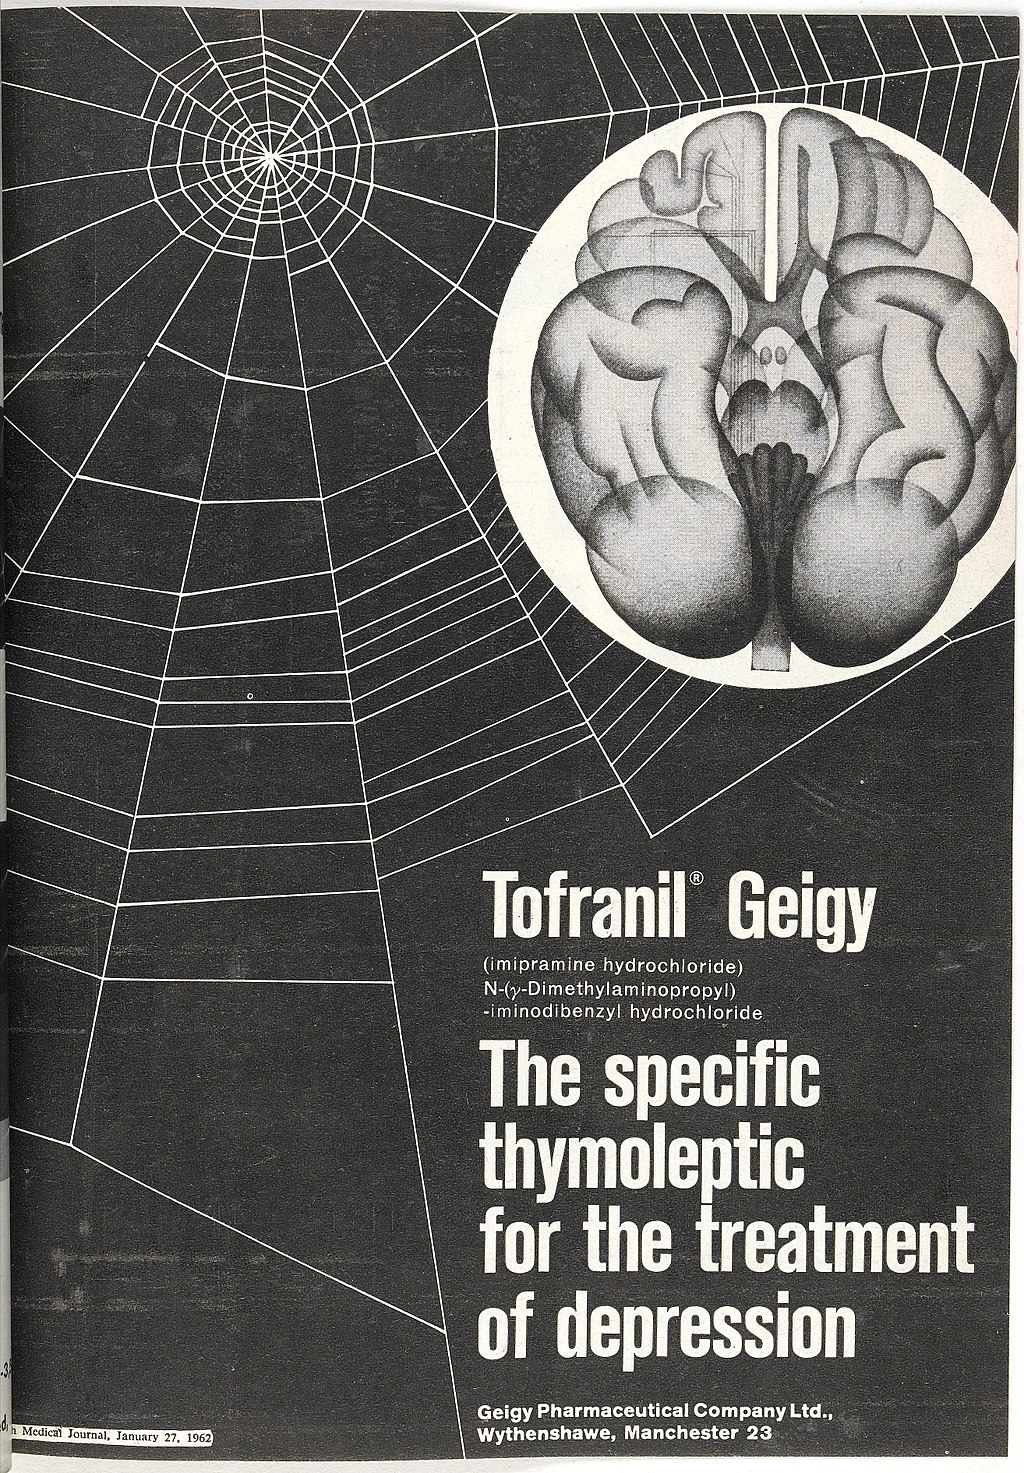
\includegraphics{../images/Trofanil_Geigy_Wellcome.jpg}
\end{center}
 \caption{See page for author CC BY 4.0  }
\label{fig: MattachinePamphlet}
\end{marginfigure}


(https:\slash \slash creativecommons.org\slash licenses\slash by\slash 4.0 ), via Wikimedia Commons https:\slash \slash commons.wikimedia.org\slash wiki\slash File:Advert\_for\_Tofranil\_Geigy\_Wellcome\_L0043517.jpg 

These drugs did—in short order—what years of psychoanalysis, hypnosis, electro-shock therapy (the decedent of Beard's treatments) and confinement could not: they allowed patients with crippling anxiety to return to normal or close-to-normal functioning.\footnote{For a particularly fascinating example, see https:\slash \slash prescriptiondrugs.procon.org\slash view.resource.php?resourceID=005707}

\section{Setting the stage for 1971}
\label{settingthestagefor1971}

In 1961, Thomas Langer and Stanley Michael conducted 2-hour interviews with 1,660 individuals chose at random from the streets of New York. This was, in many ways, the first wide-scale study of the psychology of people \emph{not already} seeking treatment for psychological trouble. Their findings are quite simple: socio-economic status and age explain most of an individual's mental health. 

The study was revolutionary. As S. H. Kranes of the University of Chicago said ``[this study] is a pioneer in obtaining `objective' information. Psychiatry is too promote to the philosophical other than the factual.'' ~\citep{Kraines:1964fy}

Since the origin of psychiatry, there has been a distinction made between those disorders that can be directly attributable to a biological dysfunction of the brain and those that cannot. The former were classified as `neurological,' and the latter `psychiatric.' It is this inability to find a biological etiology of the disorder defines the domain of psychiatry.

Two major trends are appearing in psychology and psychiatry: 

\begin{enumerate}
\item The current psychoanalytic taxonomy of mental states is based on conjectures and assumptions based on a few case studies, and they have not been tested against evidence and observation.

\item Psychiatric disorders must have a physical component, and hence, the line between psychiatry and neurology may be breaking down.

\end{enumerate}

In light of these trends, what will happen to the field of psychiatry?

\pagebreak 

\chapter{Game Play}
\label{gameplay}

\section{Major Issues in the Game}
\label{majorissuesinthegame}

All psychological theories hold that human action can be described, understood, predicted and controlled based on previous actions or mental processes of that human. The way to make those predictions---and the underlying mechanisms posited that explain those actions---separates psychological theories from each other.

When I say ‘mechanism’, I am using a very specific notion in the Philosophy of science. A mechanism is an organization of underlying entities which interact with each other to create the phenomenon of interest. Biologists talk of “mechanisms of cell death”, Doctors and Pharmacists of “drug actions and mechanisms”, Chemists speak of the “mechanisms of reactions,” etc. 

When one looks at the history of psychological theories, it is not hard to see the metaphorical connections between the psychological mechanisms posited at a certain time, and the most complicated machines available to that society. Psychoanalysis, which was dominants in American Psychiatry from 1890 until the events of this game, posits an underlying unconscious, which ‘boils’ away, providing energy for all observable behavior. When that behavior is correctly directed with the right set of pressures, it moves the organism forward. When it is not, either the pressure goes out sideways, creating negative behaviors, or it builds towards ultimate ‘explosion’ in psychosis. It is, in short, a steam engine.

Behaviorism sought to explain all behavior in terms of stimulus and response, without recourse to ‘internal states’ or ‘processes’. Behaviorism’s rise which started in 1913 and peaked with the Radical Behaviorism of Skinner in 1958 correspond roughly to the electrification of the United States, as well as the rise of mass media including radio and television. Electric lights, toasters, radios and TVs are straightforward stimulus-response mechanisms: apply electricity and something happens. Don’t apply electricity and nothing happens. The wiring is relatively simple, without internal computation or representation. 

On the other hand, once the notion of a ‘computer’ with internal working memory (RAM) and permanent storage (hard drives) arrives in the 1960’s, Cognitivism results. And notably, from MIT. Here, the mind is a metaphor of the computer: it takes information in, executes computational functions, and produces behavioral output. Today, we use computer-based nomenclature when talking about the mind all the time: someone might not have the ‘bandwidth’ for a new task, the ‘executive function’ system might be down, we look for ‘expert systems’, or think ‘algorithmically.’ These are all metaphors---metaphors that compare the human mind to the dominant technological apparatus of our time: the computer and internet.

\subsection{The Central issues}
\label{thecentralissues}

There are three interweaving threads of debate in this game. The first---the \textbf{main issue of debate}---is whether or not psychoanalysis is a viable theory of human action. If it is, mental illnesses out to be classified according to the competing psychoactive mechanisms. If it is not, we need to figure out how mental illness should be classified.

The issue of the demedicalization of homosexuality, which begins this debate, is merely the tip of the iceberg---if homosexuality is not a mental illness---a medical condition---psychiatry must address the viability of psychoanalysis and the need for psychological observation of individuals \emph{not} in already in treatment.

The second is research. Throughout the game, individuals will propose studies to the ‘Research committee.’ If they are approved, the class will break into a ‘lab’ session and conduct that research. The propose \emph{must} then report the findings at the next conference.

The third is the responsibility science has society. Obviously, the demedicalization of homosexuality was motivated because psychiatrists became aware that the stigma of ‘mental illness’ was doing more harm than good---it was causing mental illness, not curing it. But the Goldwater affair, and the Supreme Court’s citation of Kenneth Clark’s work on children internalizing prejudice in the \emph{Brown v. Board of Education of Topeka Kansas} decision weigh heavily on the Psychological and Psychiatric communities.

Table \ref{table: majorissues} summarizes these and other issues that may arise during the course of the game. As with all Reacting Games, other than the first issue---demedicalization of homosexuality---when and how these issues appear is a matter of game play, so the schedule is ultimately up to you.

 \begin{longtable}[!t]{ | P{7cm} | P{2cm} |  P{2cm} | }
\hline

\tahead{Issue}&\tahead{Partisans}&\tahead{Session} \\ \hline \hline
Homosexuality \emph{is / is not} a mental disorder&Spitzer, Socarides, Bieber, Marmor& Week 1, session A. \\ \hline
The ‘medical model’ \emph{is / is not} a suitable approach to understanding the human mind&Albee, XX& \\ \hline
Psychoanalysis \emph{is / is not} scientific.&& \\ \hline
Mental disorders should be classified according to \emph{observable symptoms / underlying mechanisms}.&Spitzer, XX psychoanalyst& \\ \hline
Mental illness / mental disorder \emph{are / are not} genuine medical conditions.& & \\ \hline
How do we define a mental illness / disorder---regardless of whether it is or is not a medical condition?&Spitzer, Szasz, Albee XX& \\ \hline
The mentally ill \emph{must / should be} treated exclusively by \emph{psychiatrists / psychiatrists} and \emph{psychologists / exclusively psychologists} &Albee& \\ \hline
What does scientific research on the mind look like? & & \\ \hline
What are the ethical limitations on psychological / psychiatric research?&& \\ \hline
What is the proper role of an intellectual---specifically a social scientist---in a democratic society?&Clark, Chomsky, Tyler& \\ \hline
\caption{Major Issues for debate}
\label{table: majorissues}
\end{longtable}

Note that while these questions overlap, none of them ought to determine any of the others. One could believe, for example, that psychoanalysis is scientific, but \emph{bad} science. Or one could believe that the medical model \emph{is} a suitable approach, but classifying mental disorders under any criteria is a mistake. The range of positions on these issues can be found in the characters in this game.

\section{Basic game play}
\label{basicgameplay}

Each week (two or three sessions, depending on your schedule) of game play reenacts one annual conference of the APA in the early 1970s. The five weeks of game play cover the years 1971--1975. In reality, these conferences are huge events. There are presentations on current research, symposia on issues facing the discipline, administrative meetings for various committees, public discussions and votes on proclamations, and publishers promoting their products. In game play, players will present papers, propose research projects, vote on resolutions and grants, and hold committee meetings.

Each conference opens with a presidential address. The position of President is both an honorific and administrative position. The President is often elected based on his or her reputation as a researcher, but he or she also must have keen leadership skills and knowledge of the policies and procedures of the organization's committee structure. Since these two areas of expertise do not always appear in the same person, an individual is \textbf{not} elected directly to the Presidency by the membership. Rather, the membership holds an annual election for the \textbf{Vice-President,} who is then promoted to President after a year of sitting on the Board of Directors and observing the inner workings of the political system. After a President’s year in office, he or she becomes the \textbf{Former President} and continues to serve on the Board.

The Board of Directors is composed of the President, the Vice president, the Former President and \emph{two} members elected at large each of whom serving three year terms. For classes smaller than 16, the Board of Directors will be limited to the current President, the Vice President and the Former President. The executive secretary, who serves without vote, is responsible for maintaining the minutes of the Board of Directors and taking whatever actions the committee approves during its meetings.

At each year's conference, the following events occur:




\begin{enumerate}

\item Presidential Address \newline
\item  Board of Directors circulates proposals to be considered by the membership. \newline
\item Symposia on topics proposed by membership, as scheduled by the program committee \newline
\item  Open sessions for presenting current research (papers or plenary addresses), as scheduled by the program committee. \newline
\item  Board of Directors meets in open session. \newline
\begin{enumerate}
    \item  All committees and task forces report \newline
    \item  Old Business (tabled from previous meeting) \newline
    \item  New Business \newline
\end{enumerate}
\item  Discussion of any proposals circulated in step (2) \newline
\item  Create and administer ballots for proposals. \newline
\item  Election for vice president, who assumes that position at the close of that conference \newline
\item  Election for member-at-large on the executive committee (if necessary) \newline
\item  Executive committee meet in closed session, if necessary. \newline
\end{enumerate}

 %\captionof{InfoBox}{Sample schedule of events for APA conference\label{sample:conference}}


 

Game play may take many forms in the classroom. You may be questioning the President about his or her vision for future directions in psychological or psychiatric research, engaging with or participating in a symposium with two or three of your colleagues on a contentious issue of the day, participating in research, evaluating research results, discussing proposals in committee, or even arguing about reports from task forces. The schedule of events will be left to the Program Committee, so it is very important that they distribute the schedule early and widely. See Section ‘\fullref{programcommittee}’ for more on the potential forms of conference activities.

\section{Basic Principles}
\label{basicprinciples}

Academic associations like the APA not only provide their members with a forum through which they can socialize, share ideas and test or their most recent work; they also represent their discipline to the public. An association's President is often called upon to act as a spokesperson during times of controversy. And the associations often define---sometimes very carefully---the qualifications someone must have to become a member.

During 1970s, the APA is being called upon to represent their membership in both of these ways. It is important, therefore, to ensure that actions of the APA---whether it be the election of a new President or the publication of a statement---represent the will of the membership. The association exists to serve the membership, not the other way around.

\subsection{Credibility Points}
\label{credibilitypoints}

In academic culture, reputation is capital. But unlike other reputation-based cultures, your reputation depends entirely on the quality of data you produce, your creativity and insight in designing research, and your ability to explain the ideas in clear, simple terms. 

At the beginning of each conference (i.e. Week), each member of the APA is given one ‘credibility point' in the form of a small slip of paper. Credibility in academic life is capital---those with it have power, those without it do not.

In this game, we treat ‘credibility’ like a currency. Each player starts with a different amount, depending their publication record so far. Players \emph{gain} credibility by presenting papers or research proposals that are of interest to other players, or by serving in positions of power, such as the President or Committee chair.

At the end of each week (one “conference”), each player must give a credibility point to the speaker they believe presented the best paper, or the best research proposal. No player may keep the weekly credibility point for himself or herself. 

When an individual retires from a formal position (President, committee, etc.) the members of that board or committee can confer upon that person a ‘gift’ of credibility points for his or her “distinguished service to the APA”. The members of the board \slash  committee who are voting on this award must do so unanimously. They must must work with the game master to determine how many credibility points to give, but no one shall be given more than 5 for distinguished service.

Credibility points, once awarded, \emph{can} be stockpiled by faction or bartered with other players. They can be traded, hoarded, used for bribes, pressure, blackmail, etc. In short, all the things that money is used for in the real world. But, just like credibility in the Academia, they have no value outside the game.

Running for various positions ‘costs’ you credibility. In game play, you must turn in the equivalent number of credibility points when accepting a nomination or declaring that you will run. These are non-refundable.

There is much to be gained in having a position of power---including more credibility when you complete your distinguished service, but it takes credibility to get credibility. The chart below is suggested, but may be modified by the Game Master.

\begin{longtable}[!t]{ | P{7cm} | P{2cm}  | } \hline
\tahead{Position}&\tahead{Cost} \\ \hline 
Vice-President of the APA& 10 \\ \hline
Member of the Board & 5 \\ \hline
Chair, Research Committee & 3 \\ \hline
Chair, Nomenclature Committee & 3 \\ \hline
Chair, Program Committee & 1 \\ \hline
\caption{Credibility ‘costs’ for service to the APA}
\label{table: credibilitymenu}  
\end{longtable} 

See \fullref{committeestructure} for a description of the structure and responsibilities of of each committee.

In the final vote (see `Victory Objectives' below), the credibility points can be turned into votes—although the specifics are left to the game master to decide. 

\subsubsection{Reputation \& Replication}
\label{reputationreplication}

Even as you strive for more credibility, reputation is paramount. Disagreements are always professional: you can disagree vociferously with an opponent, yet respect his or her abilities as a scientist. Attacking a fellow member personally, or using obvious rhetorical fallacies can damage your credibility. In game play, the board can vote to ‘censure’ a member \emph{at any time} and strip him or her of acquired credibility points. A simple majority will do.

At some point in your life---probably 7th grade---you were told that `The Scientific Method' consists of creating hypotheses, designing experiments to test those hypotheses and then formulating a new hypothesis that can be tested. But most importantly, you were probably told that scientific inquiry is distinguished from non-scientific inquiry insofar as scientific inquiry can be replicated by a stranger. 

That may be true, but notice that these claims are almost always made with the modal verb `can.' The sad truth is that few, if any, attempts at replicating scientific studies ever occur. The academy is not set up to encourage studies that reproduce known results. At educational institutions, tenure requirements force scientists to concentrate on producing novel results. Industries employ scientists to create new drugs, new techniques and new treatments, not to check the results of old ones. And practitioners are usually so swamped with the demands of their clientele that they may not be able to engage in research at all, let alone focus on replicating someone else's research.

All of that means that the academic culture relies heavily on reputation. It is generally assumed that academics are honest and that their results could be replicated, but will not be. Many people just assume that the prestigiousness of one’s academic post reflects the reliability of their results---it really is easier to publish a paper if you are from Harvard than if you are from a middle-tier public institution.

Conferences, such as the APA, rely on a system of peer review to ensure that the papers presented represent the best research available. But peer reviewers are often selected in virtue of their reputation for rigorous research and high standards. Members are elected to positions of leadership because of their reputation as psychologists or psychiatrists, not because of their knowledge of the rules of order for a public meeting. As you propose new research and present your findings at the conferences, remember that what counts is not entertainment value or charming banter, but quality of insight and rigor in data collection.

\subsection{The Responsibilities of the President}
\label{theresponsibilitiesofthepresident}

While the presidency of the APA is largely an honorific position, it does come with some serious responsibilities. It is awarded by election of the membership, according to standards known only to them. Traditionally, it has been given to significant figures in the field at the end of their careers as a kind of `lifetime achievement' award (for example, Koffka in 1958) and advocates for new and promising avenues of research early in their careers. The first president in this game, George Miller, best exemplifies the latter sort.

The President's main responsibilities include presiding over the meetings of the Board of Directors, and opening each conference with a plenary address. These addresses provide the President a huge forum to reflect on recent trends in the discipline and potential future directions.

In reality, all Presidential addresses of the American Psychological Association are published in the \emph{American Psychologist}, which is available at Jstor.org. Potential presidents should consult the journal for examples.

\section{Victory Objectives}
\label{victoryobjectives}

The game normally `ends' with a decisive vote on the definition of `Mental Illness,' probably in 1975. There are three basic definitions that ought to be advanced, which are included in table \ref{table: definitions}.
 \begin{longtable}[!t]{ | p{2cm} | p{12cm} | }
\hline

\textbf{Advocates}&\textbf{Definition}\\ \hline
APA Task Force&A Medical disorder is a relatively distinct condition resulting from an organismic dysfunction which in its fully developed or extreme form is directly and intrinsically associated with distress, disability, or certain other types of disadvantage.  The disadvantage may be of a physical, perceptual, sexual, or interpersonal nature. Implicitly there is a call for action on the part of the person who has the condition, the medical or its allied professions, and society.

A mental disorder is a medical disorder whose manifestations are primarily signs or symptoms of a psychological (behavioral) nature, or if physical, can be understood only using psychological concepts.\\ \hline
Behaviorists& A person can be called 'mentally ill' when he or she exhibits emotional or behavioral functioning which is so impaired as to interfere substantially with his or her capacity to function in society. \\ \hline
Psychoanalytic&A person is mentally ill when he or she suffers from internal conflicts that may be subconscious or unconscious, manifesting behavior that is unwanted or disturbing to the individual or the society. \\ \hline
Szasz&There is no 'thing' called 'mental illness,' only  sets of behaviors that may be destructive to an individual and his or her society. \\ \hline
 
\caption{Factional Definitions of Mental Illness}
\label{table: definitions}
\end{longtable}

Factional affiliation and objectives vary from individual to individual.

\section{Special Rules}
\label{specialrules}

If possible, each player must serve on at least one committee at some point during the game.

\subsection{Writing Tasks}
\label{writingtasks}

Every player will write and present at least once during the course of the game. Your role sheet should specify the specific tasks you need to complete.

A special note for data-driven writing tasks: don't say `studies have shown that' or (in the 1st person) `I have shown that{\ldots}', show it. That will probably mean that you will have to go to the library, find the original research reports of your character, and familiarize yourself with the basic research design, as well as the relationship between the evidence presented and the thesis that evidence is reported to support. If that sounds like a great deal of effort, it should. Above all, remember that you're not writing a report on this person or position, you are playing the person and defending the position. So don't write about what you (as the character) believe, write as if you believe it.

\subsection{Proposals to the Board}
\label{proposalstotheboard}

Proposals should be formal. They should be distributed to the membership at least 24 hours before a vote is called. It is usually sufficient to distribute proposals during the first session of a conference year, and hold a vote during the second (or third). Ample time for discussion should be allotted for each proposal. 

Formal proposals begin by laying out the reasons for the proposal with a series of `WHEREAS{\ldots}' clauses. It should then state the resolution. For example, in 1969, the APA resolved:

\begin{quote}

\emph{WHEREAS} in many state legislature, bills have recently been introduced for the purpose of repealing or drastically modifying the existing criminal codes with respect to the termination of unwanted pregnancies;

and \emph{WHEREAS} termination of unwanted pregnancies is clearly a mental health and child welfare issue, and a legitimate concern of APA;

\emph{BE IT RESOLVED} that termination of pregnancy be considered a civil right of the pregnant woman, to be handled as other medical and surgical procedures in consultation with her physician, and to be considered legal if performed by a licensed physician in a licensed medical facility.
\end{quote}

You should follow this format when drafting your proposals. Proposals in the incorrect format cannot be distributed.

\subsection{Papers and Symposia}
\label{papersandsymposia}

Academic conferences are opportunities to discuss and disseminate information you have gathered to support your views. The method of presenting those ideas or that data, however, can vary a great deal. The APA currently supports two kinds of presentations: Individual Reports and Symposia. Individual Reports are talks given by a single researcher or group of researchers. Symposia are `panel' presentations, where a group of presentations are offered on a theme or a specific problem.

The Program Committee (see \fullref{programcommittee}) is encouraged to experiment with new kinds of presentations, including posters, round tables, workshops, and even exhibits, if they choose. 

The Program Committee reviews all proposals for both individual reports and symposia. The guidelines for proposing a report are included in the official \fullref{callforpapersandsymposia}.

\subsection{Research Grants}
\label{researchgrants}

Research grants are 1--2 page proposals specifying a research project you'd like to carry out. These are submitted to the Research committee (see \fullref{researchcommittee}) and follow the form specified in the ‘Call for Research Grants', which follows on \fullref{callforresearchgrants}. If you win a research grant, you will be expected to present your findings at the annual conference that immediately follows the successful completion of your grant.

\subsection{Reading aloud}
\label{readingaloud}

Presentations at academic conferences are evaluated by peers primarily on the basis of the content presented, not the style of presentation. While it is important to practice good public speaking skills---making eye contact with the audience, modulating one's voice, etc.---getting the data right is more important than being entertaining. For that reason, this game will allow `reading' of some experimental reports. Experimental reports highlight the data presented, and carefully articulate the structure of the experiment performed. It is also advisable to bring handouts of any important charts or datasets for the membership when presenting data. 

Note that we’re in 1975, so powerpoint will not be allowed. You can, with the approval of the game master, requisition an overhead projector and print our data or charts on transparencies.

Presidential addresses, however, should be carefully crafted general lectures. These should appeal to the membership of the APA, which includes many individuals from a variety of backgrounds. They should also be understandable by the general public, as the President is often seen as a spokesperson and advocate for the discipline.

Symposia and presentations to the committees, however, must be delivered without a transcript. Cue cards or notes are allowed, but in these cases, the speaker must strive to make a personal connection with the audience, and hence, must not simply read a prepared speech.

\section{Definitions used by the APA}
\label{definitionsusedbytheapa}

The following are quoted from current websites of the American Psychological Association and the American Psychiatric Association.

\subsection{Definition of ``psychologist''}
\label{definitionofpsychologist}

APA policy on the use of the title ``psychologist'' is contained in the General Guidelines for Providers of Psychological Services, which define the term ``Professional Psychologist'' as follows:

\begin{quote}

Psychologists have a doctoral degree in psychology from an organized, sequential program in a regionally accredited university or professional school.
\end{quote}

The APA is not responsible for the specific title or wording of any particular position opening, but it is general pattern to refer to master's-level positions as counselors, specialists, clinicians, and so forth (rather than as ``psychologists''). In addition, it is general practice to refer to APA accredited programs as ``APA-accredited'' rather than ``APA approved.'' The position as described must be in conformity with the statute regulating the use of the title psychologist and the practice of psychology in the state in which the job is available.

\subsection{Definition of ``psychology''}
\label{definitionofpsychology}

Psychology is the study of the mind and behavior. The discipline embraces all aspects of the human experience — from the functions of the brain to the actions of nations, from child development to care for the aged. In every conceivable setting from scientific research centers to mental health care services, ``the understanding of behavior'' is the enterprise of psychologists.

\subsection{Definition of “psychiatrist”}
\label{definitionof“psychiatrist”}

A psychiatrist is a physician who specializes in the diagnosis, treatment, and prevention of mental illnesses and substance use disorders. It takes many years of education and training to become a psychiatrist: He or she must graduate from college and then medical school, and go on to complete four years of residency training in the field of psychiatry. (Many psychiatrists undergo additional training so that they can further specialize in such areas as child and adolescent psychiatry, geriatric psychiatry, forensic psychiatry, psychopharmacology, and\slash or psychoanalysis.) This extensive medical training enables the psychiatrist to understand the body's functions and the complex relationship between emotional illness and other medical illnesses. The psychiatrist is thus the mental health professional and physician best qualified to distinguish between physical and psychological causes of both mental and physical distress.

\newpage

Sample call for papers and symposia.\footnote{This entire section is adapted from the “Call for Papers and Symposia” from the 1957 \emph{American Psychologist}.}


\begin{apatextbox}{Sample call for proposals for APA conference}  

\rowgroup{

\subsection{Call for Papers and Symposia } \\}
\label{callforpapersandsymposia----}

\rowgroup{

\subsubsection{Introduction} \\}
\label{introduction----}

\rowgroup{ I. The Program committee herein announces a Call of Papers and Symposia for the annual convention of the APA. Please read the relevant rules carefully if you plan to take part in the program. \emph{Note especially the deadlines, the form for abstracts of contributed papers, the forms for symposium proposals, and the proper persons to receive your correspondence.} The pertinent references have been collected into the box on this page for your convenience.} \\

\rowgroup{This year will begin with a plenary address by the President. Current plans allow for 2 individual reports and 1 symposium. The Board of Directors will meet in open session to hear proposals from the membership.} \\
\rowgroup{ 

\subsubsection{Kinds of Programs and Sessions} \\}
\label{kindsofprogramsandsessions----}

\rowgroup{The meetings regularly contain many kinds of programs and sessions, including research papers, symposia, group discussions, addresses, business meetings, and film sessions, as well as other events, such as reunions, dinners, social hours and the like. In general, requests for information should be submitted to the Program Committee.} \\

\rowgroup{The APA Program Committee has full responsibility for the conference program. Persons planning to submit proposals that fall outside the lines outlined herein should consult with the chairman of the APA Program Committee for special instructions.} \\

\rowgroup{The chairman of the APA Program Committee should also receive all requests for scheduling of nonsubstantive program activities such as reunions, dinners, social hours, headquarters space, luncheons, and the like. To insure publication in the program all requests must be received by the close of business on the Friday before a conference.} \\
\rowgroup{ 

\subsubsection{Who may participate} \\}
\label{whomayparticipate----}

\rowgroup{

\paragraph{Volunteered Papers} \\}
\label{volunteeredpapers----}

\rowgroup{Any member of the APA may read a paper, provided that it has been accepted by the program committee.} \\

\rowgroup{

\paragraph{Non-members} \\}
\label{non-members----}

\rowgroup{ A non-member of the APA may read a paper provided that he is sponsored by a member of the APA and provided that his qualifications and the quality of his paper are acceptable to the program committee. The APA member who agrees to sponsor a nonmember must submit the abstract of the nonmember's paper to the chairman of the program committee with an accompanying description of the nonmember's scientific qualifications plus the names of recognized scientific societies in which the nonmember holds membership.} \\

\rowgroup{

\paragraph{Symposia and invited addresses} \\}
\label{symposiaandinvitedaddresses----}

\rowgroup{The program committee may invite distinguished nonmembers to contribute to the program as special speakers or as participants in symposia. Because symposia often involve topics extending beyond the competence of APA members, it is frequently desirable to include nonmembers as participants. Acceptance of a distinguished speaker or of a symposium proposal by the Program Committee constitutes the require sponsorship of nonmember participants.} \\
\rowgroup{

\subsubsection{Limits of Individual Participation} \\}
\label{limitsofindividualparticipation----}

\rowgroup{Over the past several years the APA's Board of Directors working with the program committee has developed several ground rules for the limits of individual participation in the annual convention program. These rules were designed to ensure the widest possible participation by APA members and also to prevent troublesome conflicts in the time schedule. Briefly, the rules have been that each member may present no more than one volunteered paper and that each member may, in addition, participate in no more than one additional session such as a symposium, discussion group, and the like. It is still strongly recommended that maximum participation be limited to one symposium or discussion group plus one paper.} \\

\rowgroup{

\subsubsection{Individual Reports} \\}
\label{individualreports----}

\rowgroup{Unless otherwise indicated, four ten-minute papers will be scheduled for each 50-minute session. In instances of multiple authorship the person whose name is listed first will be expected to present the paper.} \\

\rowgroup{A paper previously read at the Annual APA Convention may not be read again, unless it is a substantial elaboration (additional findings, etc.). Two papers which report highly similar findings from a cooperative project may not be read at the convention.} \\

\rowgroup{The APA Board of Directors have voted that, for reasons of economy, this rule should be followed: Abstracts printed in the American Psychologist are limited to 100 words. However, it is recognized that more detailed information will be needed by the Program Committee for use in the selection of papers. The procedures for research reports and other individual reports are described below.} \\

\rowgroup{

\paragraph{Research Reports} \\}
\label{researchreports----}

\rowgroup{\emph{Each author of a research report must submit a 100-word abstract (1 copy) for publication if the paper is accepted, and also a 300-word summary (4 copies) for committee publication.} If the author desires, tables presenting results may be submitted with the 300-word summary. Not more than one page of tables should be submitted. This means that all the data should have been obtained and the analysis completed at the time the abstract and summary are submitted to the Program Committee.} \\

\rowgroup{

\paragraph{Other individual reports} \\}
\label{otherindividualreports----}

\rowgroup{Theoretical papers, case studies, and the like are perfectly acceptable for the program. \emph{The 100-word abstract of a non-experimental paper must, however, be accompanied by a manuscript of the complete paper in draft form.} The complete manuscript is required in order that the Program Committee may be in a better position to judge the contribution to the program.} \\

\rowgroup{

\paragraph{Form of abstracts and summaries} \\}
\label{formofabstractsandsummaries----}

\rowgroup{All abstracts and summaries must be typed on one side of the paper only, double-spaced throughout and on 8 1\slash 2” X 11” paper.} \\

\rowgroup{

\emph{The 100-word abstract}} \\

\rowgroup{The purpose of the published abstract is to provide information concerning the psychological relevance of the paper. .. primarily to justify its scientific validity. Hence abstracts should be concerned with content … rather than with method and technique unless the purpose of the paper is essentially methodological). Examples of good short abstracts from many different fields may be found in \emph{Psychological Abstracts}.

Abstracts must be limited in length to 100 words (not counting title, author and institution). Longer abstracts will not be printed but will be listed by title only. Abstracts should not contain tables, drawings, footnotes, or bibliographic entries, as such material will not be printed.

The following outline should be followed in preparing the abstract:} \\

\rowgroup{
\begin{tabular}[!t]{ | L{6cm} | L{6cm} | }
\hline
\multicolumn{2}{| P{12cm} |}{Title of Paper: } \\ \hline
Author(s): &Sponsor (if any):  \\ \hline
\multicolumn{2}{| P{12cm} |}{Institution(s): } \\ \hline
\multicolumn{2}{| P{12cm} |}{\rule{0pt}{50pt}\emph{Text of abstract} (not to exceed 100 words)} \\ \hline
\end{tabular} 
} \\

\rowgroup{Because the 100-word abstract will be sent to the printer, do not underline or type anything with all capital letters. The type written abstract should be checked and proofread carefully, since it will be printed in the form in which it is submitted. Authors are urged to give careful thought to the visual aides that will best facilitate presentations of their data. If slides are used, members are urged to consider presenting graphic and tabular material on paper. As a new procedure, authors of accepted papers will be asked to indicate their preference for audio-visual support.} \\

\rowgroup{

\emph{The 300-word summary}} \\

\rowgroup{The text of the summary will normally include a statement of the problem, subjects used, procedure, results and conclusions.} \\

\rowgroup{Summaries must be limited in length to 300 words (not counting title, author, and institution). The 300-word summary may be accompanied by not more than one page of supplementary tables, drawings, footnotes, etc.} \\

\rowgroup{The form for submitting the 300-word summary should be exactly the same as for the 100-word abstract except, of course, for the longer text.} \\

\rowgroup{Four copies of the 300-word summary and the supplementary tables, etc. are required. \emph{Author, sponsor, and institution should appear on the first copy only.} The first copy is the one that will be used by the Program Committee Chair in the creation of the Conference Proceedings. The other three copies without identifying data will be used by the Program Committee for judging the acceptability of the paper.} \\

\rowgroup{

\paragraph{Where to send abstracts and summaries} \\}
\label{wheretosendabstractsandsummaries----}

\rowgroup{Copies of the abstract and summary of a volunteered paper should be sent to the chair of the Program Committee.} \\

\rowgroup{

\subsubsection{Symposia} \\}
\label{symposia----}

\rowgroup{A symposium provides for several prepared papers on a single theme or problem. It is an excellent form of meeting if the aim is to bring to an audience several diverse or even contradictory views, presented by a number of “experts.” The expectation would be that all papers would first be read; then there would be a substantial period for interchanging of views among the speakers (and invited discussants, if desired); finally, a brief period for questions or points raised from the floor. It is important to plan the time so that there is real interaction among participants after the papers. In order to realize the unique value of the symposium the chairman should select speakers at an early date, arrange for the participants to exchange papers ell in advance of the session, and ensure that ample time is allotted for discussion among the participants and contributors from the audience} \\

\rowgroup{

\paragraph{Initiation of symposia} \\}
\label{initiationofsymposia----}

\rowgroup{Any member of the APA may suggest a symposium topic to the chairman of the Program Committee. Such proposals must be made at an early date as a successful symposium requires much planning and correspondence. A member may also submit a fully organized symposium for the Program Committee's consideration.} \\

\rowgroup{

\paragraph{Form of symposium proposals} \\}
\label{formofsymposiumproposals----}

\rowgroup{

\emph{Suggestions to the Program Committee}} \\

\rowgroup{When a member only suggests but does not organize a symposium, he should indicate the title of the topic for discussion, comment on the significance of the topic, and list the names and addresses of the proposed chairman and other participants. Such suggestions should be sent to the appropriate divisional program chairman well in advance of the deadline to allow for ample time for planning.} \\

\rowgroup{

\emph{Member-Organized symposia}} \\

\rowgroup{A member may organize a proposed symposium in complete detail and present it for approval to the Program Committee. Each such proposal should indicate the title of the symposium and list the names of the chairman and participants, together with the titles of participants' contributions, if these titles are to be published. \emph{Five copies of the completed symposium plans must be submitted to the Program Committee by the deadline.}} \\

\rowgroup{

\emph{Symposia organized by the Program Committee}} \\

\rowgroup{Symposia may be organized independently by the Program Committee or in response to the requests of members.} \\

\rowgroup{

\subsubsection{Special Programs} \\}
\label{specialprograms----}

\rowgroup{The Program Committee should feel free to try new kinds of programs. Forums, discussion groups, panels, round tables, conferences, and workshops are often valuable alternatives to papers and symposia. Members are invited to send suggestions for new types of programs to the Program Committee. Special sessions should be suggested well in advance of the deadline to allow for ample time for planning. Procedures for initiating special programs should follow in general the procedures for initiating symposia.} \\

\rowgroup{

\subsubsection{Miscellaneous Meetings and Special Sessions} \\}
\label{miscellaneousmeetingsandspecialsessions----}

\rowgroup{APA boards, committees, etc. desiring business meetings must send to the Chairman of the APA Program Committee by the deadline a statement of estimated attendance, time required, time and day preferred and whether arrangements for luncheon and dinner are desired.} \\

\rowgroup{Luncheons, dinners and social hours may be scheduled for non-APA organizations if they send their request to the chairman of the APA Program Committee by the deadline. Such scheduled events will be listed in the condensed program.} \\

\rowgroup{

\subsubsection{Audio-Visual Presentations} \\}
\label{audio-visualpresentations----}

\rowgroup{APA members, commercial film producers or distributors who wish to present new films, film strips, or other audio-visual aids (including sound recordings) should make the Program Committee aware of this fact at the deadline. The committee will review and select the audio-visual materials which are to be presented as part of the APA program.} \\

\rowgroup{

\subsubsection{Exhibits} \\}
\label{exhibits----}

\rowgroup{APA members are encouraged to exhibit apparatus, teaching aids, and other materials of scientific and applied interest. Commercial agencies are invited to request arrangements for exhibits. All commercial exhibitors will be charged for space. Those wishing to arrange for exhibits must write to the chairman of the Program Committee.} \\

\end{apatextbox}
 %\captionof{InfoBox}{Sample call for proposals for APA conference\label{sample:cfp}} 

\newpage

Sample call for research grants.\footnote{This section adapts language from the mission statements of the contemporary APA (http:\slash \slash www.apa.org\slash about\slash )}

\begin{apatextbox}{Call for Research Grants} 
\rowgroup{

\subsection{Call for Research Grants} \\}
\label{callforresearchgrants----}

\rowgroup{

\subsubsection{Introduction} \\}
\label{introduction----}

\rowgroup{The Research Committee of the APA herein solicits proposals for research that will forward the disciplines of psychology and psychiatry. Note especially the deadlines, the form for abstracts of contributed papers, the forms for symposium proposals, and the proper persons to receive your correspondence. The pertinent references have been collected into the box on this page for your convenience.} \\

\rowgroup{Winners will be granted the support of the other members of the class for a period of one class session. The primary investigator must specify in the research proposal how the other students will participate: as subjects, participants, observers or confederates.} \\

\rowgroup{Winning grants will be determined by the Research Committee, in accordance with the criteria specified herein. All proposals must be in line with the APA's ethical guidelines which are in force at the time of submission.} \\

\rowgroup{

\subsubsection{Research Supported} \\}
\label{researchsupported----}

\rowgroup{The APA seeks to advance the creation, communication and application of knowledge of the mind and behavior to benefit society and improve people's lives. The APA embraces scientific inquiry into all aspects of the human experience — from the functions of the brain to the actions of nations, from child development to care for the aged. And in every conceivable setting from scientific research centers to mental health care services, ``the understanding of behavior'' is the enterprise of psychologists.} \\

\rowgroup{Additionally, the APA aspires to advance the understanding of psychology and psychiatry as scientific disciplines. To that end, it will support any research that follows the standards of scientific inquiry and contributes to the central goals of the association.} \\

\rowgroup{It is imperative that all research supported by the APA must be accordance with the ethical guidelines published by the APA. } \\

\rowgroup{

\subsubsection{Who May Submit Proposals} \\}
\label{whomaysubmitproposals----}

\rowgroup{

\paragraph{Members of the APA} \\}
\label{membersoftheapa----}

\rowgroup{Any member of the APA may submit a proposal for a research grant. APA membership is limited to those meeting the definition of `Psychologist' or `Psychiatrist' used by the APA (see p. 10 of the gamebook).} \\

\rowgroup{

\paragraph{Nonmembers of the APA} \\}
\label{nonmembersoftheapa----}

\rowgroup{As the APA Research committee seeks to further the disciplines of Psychology and Psychiatry wherever they are practiced, the primary investigator of a grant need ot be a member of the APA. The primary investigator, however, must be a Psychologist or Psychiatrist as defined by the APA (see p. 10 of the gamebook).} \\

\rowgroup{

\paragraph{Confederates, Observers and Assistants} \\}
\label{confederatesobserversandassistants----}

\rowgroup{Individuals working in psychological research should be engaged in some significant way with the academic pursuit of knowledge. Confederates, observers and assistants in research must therefore be students of psychology or psychiatry, if not psychologists or psychiatrists in their own right.} \\

\rowgroup{

\subsubsection{Limitations of Participation} \\}
\label{limitationsofparticipation----}

\rowgroup{A primary investigator may submit one (1) proposal annually. An individual may serve as a consultant, confederate, observer or assistant on any number of grant proposals in addition to proposing himself as a primary investigator. } \\

\rowgroup{

\subsubsection{Form of the Proposal} \\}
\label{formoftheproposal----}

\rowgroup{

\paragraph{Introduction} \\}
\label{introduction----}

\rowgroup{Limited to 100 words, the introduction should specify the phenomenon you wish to examine and why. Briefly describe the phenomenon in general, and discuss how it relates to the study of the human mind and behavior.} \\

\rowgroup{

\paragraph{Background \slash  Review} \\}
\label{backgroundreview----}

\rowgroup{Briefly describe the history of research into this phenomenon, and why that history is insufficient. Summarize what is already known about the phenomenon, including the background information you gleaned during your literature review.} \\

\rowgroup{

\paragraph{Rationale} \\}
\label{rationale----}

\rowgroup{Describe the questions you are examining and explore any possible implications of your study. This includes listing the specific questions you are addressing, explaining how your research is related to the larger issues raised in the introduction. Specifically describe the claims, models or hypotheses you will evaluate with your research. Explain how your research will contribute to our understanding of the mind.} \\

\rowgroup{

\paragraph{Method and Design} \\}
\label{methodanddesign----}

\rowgroup{Describe how you will go about collecting data and testing the questions you wish to examine. While novel methods are encouraged, the primary investigator must be able to specify the scientific validity of any methods proposed.} \\

\rowgroup{Method: How will you collect the data?}  \\

\rowgroup{ Describe the general methodology you choose for your study, i.e. observational, experimental, etc. } \\

\rowgroup{* Explain why this method is the best method for this question. } \\

\rowgroup{* Specify who will participate in your study, and why.}  \\

\rowgroup{* Describe the sample you would test and explain why you have chosen this sample. Include age, and language background and socio-economic information, if relevant to the design. } \\

\rowgroup{*Are there any participants you would exclude? Why, why not?} \\

\rowgroup{Design } \\

\rowgroup{* Describe what kinds of manipulations\slash variations you would make or test for in order to test your hypothesis(es). } \\

\rowgroup{* Describe the factors you would vary if you were presenting a person with stimulus sentences.}  \\

\rowgroup{* Explain how varying these factors would allow you to confirm or disconfirm your hypotheses.}  \\

\rowgroup{* Explain what significant differences you would need to find to confirm or disconfirm your hypothesis(es). In particular, how could your hypothesis(es) be disconfirmed by your data?}  \\

\rowgroup{* Controls: What kinds of factors would you need to control for in your study? } \\

\rowgroup{* Describe what types of effects would be likely to occur which would make your results appear to confirm, or to disconfirm your hypothesis(es). } \\

\rowgroup{* Describe how you can by your design rule out or control for apparent effects.}  \\

\rowgroup{Procedure } \\

\rowgroup{* How are you going to present the stimuli?}  \\

\rowgroup{* What is the participant in the experiment going to do?}  \\

\rowgroup{Analysis } \\

\rowgroup{* How will you analyze the results? } \\

\rowgroup{* What kind of results would confirm your hypothesis? } \\

\rowgroup{* What kind of results would disconfirm your hypothesis}  \\

\rowgroup{

\paragraph{Significance and Contribution} \\}
\label{significanceandcontribution----}

\rowgroup{

\paragraph{References} \\}
\label{references----}

\rowgroup{

\paragraph{Where to send your proposal} \\}
\label{wheretosendyourproposal----}

\rowgroup{Three copies of the proposal should be sent to the chairman of the Research committee.} \\

\rowgroup{

\subsubsection{Reports} \\}
\label{reports----}

\rowgroup{Research findings should be submitted to the conference committee for the annual national conference following the awarding of the grant. The primary investigator should follow the guidelines found under `Research Reports' (see \ref{researchreports} on page \pageref{researchreports}) in drafting his research report. Winning a grant in no way guarantees inclusion in the following year's conference program.} \\

\end{apatextbox}
 %\captionof{InfoBox}{Sample call for research grants\label{sample:cfg}} 

\section{Role of the gamemaster}
\label{roleofthegamemaster}

The gamemaster's central responsibility will be to ensure that the conferences run smoothly. The gamemaster must therefore maintain a robust relationship with the program committee. In a small class, the gamemaster may prefer to the responsibilities of the program committee for himself or herself.

\begin{itemize}
\item Act as secretary to the Board of Directors if there is no preceptor available.

\item Remind \slash  cajole the program committee to prepare the schedule at least 48 hours in advance of each class.

\item Maintain the election cycle (see the table in the instructor's manual)

\item Distribute research reports were appropriate.

\end{itemize}

\section{Outline of the game}
\label{outlineofthegame}

\subsection{Schedule of Game Sessions}
\label{scheduleofgamesessions}

 \begin{longtable}[!t]{ | p{2cm} | p{1cm} | p{11cm} | }
\hline

\tahead{Year---Location}&\tahead{Session}&\tahead{Activities} \\ \hline

\multicolumn{3}{ | p{14cm} | }{\tahead{1971---Washington DC}} \\ \hline
&A&Presidential Address\: George Miller \newline
Symposium: “Psychiatry: Friend or Foe to Homosexuals: A Dialogue,” (Dr H. Anonymous, E. Hooker)\newline
T. Szasz “The Myth of Mental Illness”\newline
Presentation of 'mental rotation' task: gamemaster\\
&B&Marmor “Limitations of Free Association”\newline
Proposal from J Marmor\newline
Proposal from C. Socarides.\newline
Petition from G. Albee.\newline
Research report from G. Miller on 'mental rotation' task\\ \hline

\multicolumn{3}{ | p{14cm} | }{\tahead{1972---Dallas}} \\ \hline
&A&Presidential Address\: Albert Bandura\newline
Symposium on Medical Model (G. Albee, T. Szasz)\newline
Report from taskforces\\
&B&R. Spitzer 'The Fiegner Criteria'\newline
P. Gebhard on the Kinsey reports\newline
H. Harlow 'Lust, latency and love'\newline
Research Report\\ \hline
\multicolumn{3}{ | p{14cm} | }{\tahead{1973---Honolulu}} \\ \hline
&A&Presidential Address\: \newline
Paper(s) \newline
Reports from taskforces\\
&B&Symposium\:\newline
Proposal to create “Spitzer Taskforce”\newline
[other proposals]\newline
Research Report\\ \hline
\multicolumn{3}{ | p{14cm} | }{\tahead{1974---Philadelphia}}\\ \hline
&A&Presidential Address\:\newline
Symposium\:\newline
Paper(s)\\
&B&Open hearings on proposed definition of 'mental illness'\newline
[other proposals]\newline
Research Report\\ \hline
\multicolumn{3}{ | p{14cm} | }{\tahead{1975---Chicago}}\\ \hline
&A&Presidential Address\:\newline
Open vote of the membership on definition of mental illness.\newline
Paper(s)\\
&B&Symposium:\newline
[other proposals]\newline
Research Report\\
\hline

\caption{Outline of game sessions}
\label{table: outlineGameSessions}
\end{longtable}

\subsection{Committee structure}
\label{committeestructure}

The APA is overseen by a Board of Directors, which is responsible for maintaining the organization, and approving all official public proclamations and publications of the organization. The president, who opens the conference with his or her presidential address, also serves as chair of the Board of Directors during that conference. The secretary of the Board of Directors is responsible for maintaining the minutes for that meeting and implementing whatever policy decisions are required.

In addition to the Board of Directors, there are currently three standing committees of the APA. All standing committees report directly to the Board of Directors annually at the Board meeting. All standing committees have the right to request an open session at the general conference for whatever they wish. If they want to initiate a vote by membership, however, they must file a request with the Board of Directors. If the Board of Directors approves the request, the standing committee can administer a vote.\footnote{The gamemaster may choose, depending on the size of the class, to combine these committees, or assign these responsibilities to the Board of Directors.}

\newpage

\subsubsection{Board of Directors}
\label{boardofdirectors}

\textbf{Responsibilities:}
* Hold open meetings each conference where topics can be discussed and voted upon.

\textbf{Powers:}

\begin{itemize}
\item Issue public proclamations on behalf of the membership.

\item Maintain official publications, such as the DSM

\item Create ad-hoc committees and task forces, as necessary.

\item Oversee and receive reports from the standing committees.

\item Censure---can strip any member of credibility at any time. Generally reserved for use of ad hominem attacks or other bad behavior. Any number of credibility points can be stripped.

\item Banning---rarely used, but available if necessary. Can place a lifetime ban on any member at anytime.

\item Confer 1--10 credibility points on retiring board members in recognition of their ‘distinguished service’

\end{itemize}

\textbf{Initial Membership:}

The membership of the Board of Directors is:

 \begin{longtable}[!t]{ | p{3cm} |  p{10cm} | }
\hline
\textbf{Position}&\textbf{Term} \\ \hline
President&Chair of the Board of Directors, serving a 1-year term \\ \hline
Vice-president – elected annually&Serves a 1-year term as Vice-president, automatically promoted to President for the next year at the close of that year's annual conference \\ \hline
Former President&Serves a 1-year term \emph{after} their service as the chair of the Board of Directors. \\ \hline
Executive secretary (preceptor), without vote.& \\ \hline

Committee member elected at large&Serving 3-year term. \\ \hline
Committee member elected at large&Serving 3-year term. \\ \hline
\caption{Board of Directors Membership}
\label{table: boardMembership}
\end{longtable}

A sample agenda for a meeting of the Board is available on page \fullref{sample:bod}.

The membership of the Board of Directors for the course of gameplay is contained in table \fullref{table: boardMembership}.

 \begin{longtable}[!t]{ | p{1cm} | p{2.5cm} | p{2.5cm} | p{2.5cm} | p{2.5cm} |  p{2.5cm} | }
\hline
\tahead{Year}&\tahead{Former President}&\tahead{President}&\tahead{President-Elect}&\tahead{Member at large 1}&\tahead{Member at large 2} \\ \hline
\tahead{1971}&Harlow&Miller&Bandura&Milgram&Albee\\ \hline
\tahead{1972}&Miller&Bandura&Elected 1971&Elected 1971&-\\ \hline
\tahead{1973}&Bandura&1971&Elected 1972&-&Elected 1972\\ \hline
\tahead{1974}&1971&1972&Elected 1973&-&-\\ \hline
\tahead{1975}&1972&1973&Elected 1974&Elected 1974&-\\ \hline
\caption{Terms for Board of Directors members}
\label{table: boardMembership}
\end{longtable}

The Board of Directors is one of a handful of standing committees of the APA. Standing committees are permanent institutions, whose membership is elected by the membership at large. Ad hoc (literally `after the fact') committees or `task forces' are created by simple majority vote of the Board of Directors and are tasked with generating a report on a specific problem or area of research. Usually, these are formed when the Board of Directors believes it has inadequate information on a specific subject. For the purposes of this game, ad hoc committees will conduct literature reviews on behalf of the Board of Directors and report to the membership. Ad hoc committees disband after the report is accepted by the Board of Directors. 

The Board of Directors has the power to create ad hoc committees or task forces as it sees fit. The membership of those committees may be specified directly by the Board of Directors at the time of creation, left to the chair of the newly created committee to decide, or even determined by popular vote of the membership. That decision is left to the Board of Directors.

Unlike the creation of ad hoc committees or task forces, the creation of new permanent standing committees require a majority vote of the APA membership, not just the Board of Directors. A full proposal for such a committee, specifying its membership structure, voting procedures, rights and responsibilities should be distributed to the membership at least 48 hours before the vote. Dissolving a standing committee requires a majority vote of the membership.

The Board of Directors represents the membership, it does not act in opposition. It is incredibly important, then, that the Board seeks approval from the membership as a whole at every turn. The Board is a capable of assigning duties to various subcommittees on its own, but all matters of policy should be turned over to the membership for an up or down vote.

\newpage

\begin{apatextbox}{Sample Schedule: Board of Directors}


\begin{enumerate}

\item Reports of the committees and task forces \newline
\begin{enumerate}
\item  Research \newline
\item  Nomenclature \newline
\item  Conference program \newline
\end{enumerate}
\item Old Business (any items that were tabled at previous meetings) \newline
\item  New Business. \newline
\begin{enumerate}
    \item  Discussion of any proposals already circulated \newline
    \item  Administer votes on any proposals already circulated) \newline
    \item  Elections for vice-president and expiring member at large. \newline
\end{enumerate}
\end{enumerate}

\label{sample:bod}
\end{apatextbox}

 

\newpage

\subsubsection{Research Committee}
\label{researchcommittee}

The research committee is charged with distributing grants to fund research as well as enforcing the APA's Ethical Standards in the practice of Psychology and Psychiatry (see \ref{app: APAEthics}).

\textbf{Responsibilites}

\begin{itemize}
\item Solicit proposals in the form of a `call for research grants'

\end{itemize}

\textbf{Powers} 

\begin{itemize}
\item Award grants to those proposals it deems excellent

\item Hearing and deciding on cases of research ethics, including punishments for violators up to and including removal from the APA for life.

\item Confer 1--5 credibility points on retiring board members in recognition of their ‘distinguished service’

\end{itemize}

The Research committee should solicit proposals in the form of a `Call for Research Grants' that specifies both the deadline for submissions, as well as the time frame for reviewing submissions. The Research Committee should revise the enclosed \fullref{callforresearchgrants} to suit their needs.

In the context of the game, winning a grant entitles the bearer to access the student body for a period of one class session, during which time he or she can perform his or her approved research project. After that period, the grantee will be expected to present his or her findings to the membership as a conference paper \slash  report.

The Research committee should take great care in considering the scientific value of each proposal. The APA does not want to be seen supporting poor or biased research! As such, members of the Research committee are strongly advised to carefully consult the ‘\fullref{basicscientificresearch} as well as the ‘\fullref{ethicsofhumanresearch}.

The Research committee is also charged with hearing and ultimately ruling on charges of ethical transgression. The Board alone has the power of censure, but the Research committee can recommend censure to the Board. 

The Board of Directors should hold an election each year for a new member of the Research committee. 

\textbf{Initial membership}

Members of the Research committee in 1971:

\begin{itemize}
\item L. Tyler (expiring 1972)

\item K. Clark (expiring 1973)

\item J. Marmor (expiring 1974)

\end{itemize}

\newpage

\subsubsection{Nomenclature Committee}
\label{nomenclaturecommittee}

The Nomenclature committee is charged with maintaining the official terminology of psychology and psychiatry. This is embodied by the Diagnostic and Statistical Manual, which is the definitive source for definitions and classifications of mental disorders. 

\textbf{Responsibilites}

\begin{itemize}
\item Maintain the official diagnostic and statistical manual of mental illness

\end{itemize}

\textbf{Powers}

\begin{itemize}
\item Define what kind of behaviors qualify as ‘mental illnesses’, thereby (because of the rise of health insurance and managed care) defining what kind of behaviors psychologists and psychiatrists can get paid to treat.

\item Confer 1--5 credibility points on retiring board members in recognition of their ‘distinguished service’

\end{itemize}

It determines who can be diagnosed with what, what treatments are considered responsible and what disorders will be covered by medical insurance. If a condition does not appear in the DSM, psychiatrists cannot treat patients with that condition. Given the increasing importance of health insurance in the 1970s, it is vital to have a standardized diagnostic system to support billable treatments.

Members of the nomenclature committee serve for six years.

Members of the nomenclature committee are strongly advised to carefully consult the ‘\fullref{briefhistoryofthestudyofhomosexualityinamerica}’ of the gamebook.

\textbf{Initial Membership}

Members of the nomenclature committee in 1971:

\begin{itemize}
\item G. Albee (expiring 1972)

\item J. Spiegel (expiring 1974)

\item R. Spitzer (expiring 1976)

\end{itemize}

\newpage

\subsubsection{Program Committee}
\label{programcommittee}

The Program Committee is charged with scheduling the conferences. 

\textbf{Responsibilities}

\begin{itemize}
\item Solicit proposals from the membership

\item Create the schedule for each conference

\item Confer 1--3 credibility points on retiring board members in recognition of their ‘distinguished service’

\end{itemize}

\textbf{Powers}

\begin{itemize}
\item Decide who gets to speak at any conference, thereby determining who has the ability to gain credibility.

\end{itemize}

The committee must remember that each conference opens with a public address from the sitting president, and each standing committee has the right to a session at each conference. Not all the standing committees will make use of that time, but each should be approached before the schedule is drawn up.

Proposals for symposia and presentations should be solicited from the general population. The committee meets in closed session (i.e. after class) to determine the conference schedule after reviewing all of the materials submitted. It is vitally important that the symposia and papers accepted represent the highest standard for academic work. They should be judged by that standard alone, not with respect to theoretical commitment or viewpoint. The conference schedule should be made available to the membership at least 48 hours before the conference begins (i.e. by Friday evening before a new conference).

The Program Committee is composed of three members, each of which serve three year terms. Hence, the Board of Directors must hold an election for a new member every year.

The schedule for the conference is set by the `Program Committee', but there are a number of business events that must take place each year. These are outlined in \fullref{sample:bod}.

\textbf{Initial membership}

Program committee in 1971:

\begin{itemize}
\item E. Hooker (expiring 1972)

\item A. Anastasi (expiring 1973)

\item P. Gebhard (expiring 1974)

\end{itemize}

\newpage

\subsection{Elections}
\label{elections}

The following shows elections that must be held each year, and the character vacating that position in parentheses. Characters serve through to the end of the conference in the year indicated. The VP immediately becomes the president: so while Bandura vacates the position of VP at the end of the conference in 1971, he becomes President at that moment. The election in 1971 is for the VP of 1972, who will be President in 1973.
 \begin{longtable}[!t]{ | p{1cm} | p{2cm} | p{2cm} | p{2cm} | p{2cm} |  p{2cm} | }
\hline
\tahead{Year}&\tahead{VP}&\tahead{Board at large}&\tahead{Research (replacing)}&\tahead{Nomenclature (replacing)}&\tahead{Program (replacing)} \\ \hline
\tahead{1971}& 1972: (Bandura)&A (Milgram)& & & \\
\tahead{1972}&1973&B (Albee)&(Tyler)&(Albee)&(Hooker) \\
\tahead{1973}&1974& &(Clark)& &(Anastasi)\\
\tahead{1974}&1975&A&(Marmor)&(Spiegel)&(Gebhard) \\
\tahead{1975}&1976&B&(elected 1972)& &(elected 1972) \\ \hline
\caption{Elections to be held each year}
\label{table: boardMembership}
\end{longtable}

\pagebreak 

\chapter{Roles and Factions}
\label{rolesandfactions}

\section{Main Factions}
\label{mainfactions}

Players represent three factions with different perspectives on not only the nature of scientific inquiry into the human mind, but the object of those studies themselves. A number of independents, representing a variety of academic disciplines, complement these three factions.

It should be noted that unlike some other reacting games, individuals in these factions are not bound to think or vote the same way on the central issues in the game. The factions represent high-level agreement on the nature of the science of the mind, there is almost complete disagreement on all other issues. In fact, when it comes to actual game play, you might find that your votes are more aligned with members of other factions than your own.

\subsection{Psychoanalysts}
\label{psychoanalysts}

Psychoanalysts are split in the classical (Freudian), Jungian and unspecified. The game contains a number of independent psychiatrists who, while they are familiar with psychoanalysis, are not professed members of the faction.

\subsubsection{Classical}
\label{classical}

Classical psychoanalysis can be summarized by five basic hypotheses:

\begin{enumerate}
\item First, psychoanalysts hold that the mind is composed of entities in conflict, also known as the \emph{hypothesis of intrapsychic conflict} or \textbf{dynamic hypothesis}. In classic Freudianism, the hypothesis followed “the discovery of the unconscious” by Breuer and Freud in 1895 (see \ref{hysteriaandhypnosis:freudbreueronannao.}). Traumatic event or fantasies can leave a subject with memories that are unacceptable to the conscious awareness. The conscious awareness defends itself by suppressing the traumatic event in the unconscious by means of repression (see, e.g. \emph{Introductory Lectures on Psychoanalysis}, p. 82, 94 also p. 438). This hypothesis is sometimes called the \textbf{psychodynamic hypothesis}.

\item Second, psychoanalysis posits that there is a finite amount of psychic energy available to any given individual. This forms the \textbf{Economic hypothesis} of classical psychoanalysis (See Freud, \emph{Introductory Lectures}, p. 26 and 436--7 for the thesis that psychic energy is sexual; p. 340, 442--3 and 466for an explicit statement. It also appears in \emph{On the Interpretation Dreams}, Ch7). The activities of the mind are “costly,” and hence the mind will optimize its function for the most efficient option.

\item The \textbf{topographical hypothesis} is Freud's most well known: the mind composed of three basic kinds of thoughts: conscious thoughts, pre-conscious thoughts and unconscious thoughts. The term `thoughts' here is used broadly, to include wishes, desires, fears, emotions, etc. Conscious thoughts are those of which we are aware. Pre-conscious thoughts, are not currently conscious, but are readily available to consciousness. The memory of your last birthday, for example, is probably pre-conscious, not unconscious. Unconscious thoughts, which far outnumber the other two categories, are unavailable to consciousness. All these thoughts, however, originate in experience: there is nothing in the unconscious store that is not linked in some way to that individual's past experiences. (see, e.g. \emph{Introductory lectures}, p. 25)

\item The \textbf{genetic hypothesis} claims that human behavior is best explained in terms of the original conditions that cause it. In Freud's theory, the genetic hypothesis takes the form of his theory of infantile sexuality.\\
For Freud, all behavior ultimately originates in sexual desire. To summarize briefly: Freud hypothesized that sexual drive, the main source of psychic energy, is present from birth. He is explicit in using the term `sexual' here, but it is sometimes easier to understand if we use a softer term like `using one's body for pleasure.' Freud repeated argues for infantile sexuality by pointing out the noncontroversial pleasure children take in tickling or cuddling, but we wouldn't necessarily call these `sexual' today. Freud himself, somewhat to his detriment, insisted on the term `sexual' even despite these kind of objections.\\
This drive towards physical gratification takes various forms throughout our lives, moving through the oral phase to the anal phase to the phallic stage. If the internal drives are left unfulfilled, or the internal conflicts unresolved (which is really two ways of saying the same thing), neurotic behavior results.\footnote{`Neurotic' behavior results from continuing conflict between the libidinal desires and the ego's repression techniques. `Psychotic' behaviors result when the libidinal desires assert their reality on the ego. See the discussion of `neurosis' and `psychosis' in the History of the Classification of Mental Illness section below.}

\item Psychoanalysts differ with respect to the entities that comprise the mind, but most recognize Freud's basic \textbf{structural hypothesis}: the mind is functionally divided between the id, the ego and the superego (see \emph{Introductory Lectures}, p. 365).\footnote{The Introductory Lectures were published before Freud solidified the structural hypothesis using this terminology. The beginnings of the idea, however, is present in the later chapters on neurosis: see, e.g. p. 437--438, where he describes the conflict between the `libido' and the `ego'.} The \emph{id}, which is totally unconscious, contains the representations of sexual and aggressive instinctual drives. The \emph{ego} regulates and controls the desires of the id in relation to the demands of the external world, which are internalized as the \emph{superego}. The ego follows the \textbf{economic hypothesis}, in seeking to maximize gratification of the instinctual desires while minimizing the amount of psychic energy spent in that process. It achieves this end through the use of various mechanisms of representation and repression (sometimes called `defense mechanisms'):\footnote{The Introductory Lectures mention only repression, subdivided into `condensation' and `displacement' as mechanisms of the ego, but promises further work on the topic (p. 364--366). He began to develop a taxonomy of ego mechanisms later in his life, but the full-fledged taxonomy we see here was developed his daughter Anna Freud (1936). The Ego and and the Mechanisms of Defense. C. Baines (trans). Connecticut: International University Press.}

\item \textbf{Repression}: The first mechanism proposed by Freud (Breuer and Freud), the ego banishes or precludes an idea or feeling from conscious awareness.

\item \textbf{Isolation}: Ideas are split off from their associated feelings (affect) and presented as alien or foreign in origin.

\item \textbf{Reaction formation}: replacing the unacceptable desire with its symbolic opposite.

\item \textbf{Displacement}: unacceptable wishes are removed from their original objects and moved to an acceptable, or at least not-unacceptable one.

\item \textbf{Projection}: an unacceptable idea or desire is attributed to someone else.

\item \textbf{Undoing}: painful or unacceptable ideas are minimized by overdoing some opposite action in some opposite arena.

\item \textbf{Turning against the self}: the original object of an unpleasant desire (usually hate) is replaced with the self.

\item \textbf{Denial}: the individual remains unaware of certain aspects of reality that would be painful to recognize.

\item \textbf{Rationalization}: the individual convinces himself or herself that their behavior has a logical, reasonable, or at least neutral, explanation in order to avoid the unacceptable cause.

\item \textbf{Identification}: usually found during development, a child becomes like another person (usually a parent) in order to deal with separation or loss of a love-object.

\end{enumerate}

These conflicts can be discovered by studying the mechanisms of representation that are used to obfuscate and repress traumatic experiences and latent desires. The mechanisms of representation take the object represented (the `latent content') and replace it with a representation (the `manifest content'). The relationship between these two can be one of:

\begin{itemize}
\item \textbf{Part to whole}: the latent content is fragmented and represented in isolation. (~\citep[p. 147]{Freud:QdOvAgyZ})

\item \textbf{Allusion}: the latent content is represented by, in Freud's words “a caption, as it were, or an abbreviation in telegraphic style.” (~\citep[p. 148]{Freud:QdOvAgyZ})

\item \textbf{Plastic portrayal}: the latent content is replaced with a plastic, concrete portrayal of it, taking its cue from the superficial aspects of the latent content. For example, the editor of a `Survey' may be represented in a dream as a `surveyor'. (~\citep[p.149]{Freud:QdOvAgyZ})

\item \textbf{Symbolism}: symbols are stable translations of one object into another. The relation between the object symbolized (the latent content) and the object that does the symbolization (the manifest content) is stable in an individual, but may not be stable between individuals. But it is always true that the latent content and manifest content share something in common. It is the task of the psychoanalysts, through the techniques of free association and manipulating transference reactions, to discover the common factors between the latent and manifest content, and hence reveal the symbolic relationships.\footnote{In many works, including Psychopathology in Everyday Life, Introductory Lectures on Psychoanalysis and On the Interpretation of Dream, Freud provides the following outline of the kinds of commonality that underly symbolism: that of number (i.e. `3' and male genitalia), shape (i.e. long, straight objects such as sticks, umbrellas, posts, trees represent the male organ \slash  hollowness or enclosing space such as vessels, bottles, boxes, trunks and ships symbolize female genitals; apples, peaches and fruit symbolize breasts), function (i.e. penetrating the body: knives, daggers, spears, sabers, firearms, rifles, pistols etc.; producing liquids, such as water-taps, water-cans, etc.; and being capable of lengthening or shortening, such as pencils, hanging-lamps, etc.; defying gravity (i.e. balloons, flying machines and zeppelins also represent the male organ). More complicated representations depend on personal associations with or reactions to objects: the complicated nature of landscapes mean they represent female bodies, sweets represent sexual satisfaction. Activities such as playing games, playing piano, sliding, gliding or pulling stand for masturbation because of the similarity of action. On the same note, rhythmic actions such as dancing, riding and climbing stand in for the sex act itself. Simple associations may appear as well: neckties, which are only worn by men, can symbolize men. (Introductory Lectures, p. 188--204)} (~\citep[p. 185]{Freud:QdOvAgyZ})

(see [Lecture VII-X][~\citep{Freud:QdOvAgyZ})

\end{itemize}

By revealing these relationships to the subject of psychoanalysis, the ego becomes aware of latent trauma and hence can deal with it in healthy ways, removing the conflict and obviating the neurosis.

Interpsychic conflict is a part of the normal maturation of a healthy adult mind. Neurosis and Psychosis occur, therefore, when this development goes wrong in some important way. Development can go awry through \emph{inhibition} or \emph{regression} (see ~\citep[Ch 22--23]{Freud:QdOvAgyZ}). In `inhibition', portions of function of the ego are held back from development, often because it becomes \emph{fixated} on a particular libidnal instinct. In `regression' an ego that has progressed further than a given developmental stage returns to that stage was a kind of defense mechanism.

The terms `neurosis' and `psychoneurosis':

\begin{quote}

“refer to a class of psychiatric illnesses characterized by prominent symptoms that have no significant somatic origin. The symptoms include disturbances of feelings (anxiety, depression, guilt), disturbances of thought (obsessions), and disturbances of behavior (compulsions and phobic inhibitions), all of which are experienced as alien to the comfort and well-being of the individual” (\emph{American Handbook of Psychiatry}, p. 737--738)
\end{quote}

Neurosis, then, is explained when the conflict between the desires of the id and the defense mechanisms of the ego go awry: (1) the ego's defense mechanism leaves the drive unfulfilled, (2) the defense mechanism imposes a disguised or symbolic form onto the original drive in order to hide it from the consciousness, and (3) the superego imposes some suffering as punishment for the self-denial, such a guilt.

Psychosis occurs when the id constructs its own reality and imposes it on the ego. The subject can no longer function in normal life—he or she may be beset by hallucinations, persistent delusions, wild mood swings, visual and auditory agnosia, amnesia, etc. It is worth noting that unlike \emph{neuroses}, psychoses may be the result of organic brain syndromes or other physical conditions.\footnote{see 290--294 of the DSM II, which is included in Appendix \fullref{app: DSMII}.} Psychoses not associated with physical conditions include schizophrenia, affective disorders and other reactions.\footnote{see 295--299 of the DSM II}

As the id is the source of psychic energy, unacceptable drives using one of the mechanisms above will not remain repressed forever. As unacceptable drives gain in strength and threaten to reveal themselves, a number of reactions are possible (see \emph{Introductory Lectures}, Ch. 19):

\begin{itemize}
\item \textbf{Anxiety reaction}: a chronic, free-floating anxiety which may have periods of acute anxiety. Typified by feelings of helplessness; although symptoms include phobias, obsessions, compulsions and depression. It is caused by the failure of all the defenses to keep the unacceptable instinctual drives in stable control. (\emph{Introductory Lectures}, Ch. 25, p. 452)

\item \textbf{Phobic reaction}: typified by one or more prominent phobias: and extreme anxiety focused on an ordinary place, object or situation. The mechanism of displacement moves the anxiety associated with the unacceptable drive to a neutral place, object or situation, which then is allowed to flourish unchecked by the defense mechanisms of the ego. (\emph{Introductory Lectures}, p. 495--498)

\item \textbf{Conversion reaction}: what used to be called `hysteria', it can manifest itself in many symptoms, including spasms, temporary paralysis, visual or auditory agnosia, weakness, shortness of breath, pains, etc. It results when the unacceptable instinctual drive is `converted' into apparently physical symptoms. (\emph{Introductory Lectures}, p. 485, 497--8)

\item \textbf{Obsessive-compulsive reaction}: the patient is troubled by persistent thoughts that are usually painful in nature. These obsessional thoughts interfere in some important way with the patient's ability to engage in a meaningful adult life: i.e. intellectually, sexually, socially or professionally. Anxiety at not following through on an obsessional thought, which often manifests as repeated actions regarding some mundane object, can be severe and often is only revealed by completion of the mundane task in question.\footnote{See item 300 in the DSM II for the full taxonomy of neurosis.} (\emph{Introductory Lectures}, Ch. 17)

\end{itemize}

As an example, classical psychoanalysis holds that obsessive-compulsive reaction can be traced to unresolved conflicts in the anal stage of development, where frustration at potty-training is turned into rage towards one's mother. That rage, in turn, is found to be unacceptable by the ego and repressed through one of the standard mechanisms creating obsessions with objects or scenarios that are symbolically linked to the original frustration. The particular object of obsession is essentially random, as the subject latches onto some mundane object present at the time of the frustration. The choice of obsessional object, however, can provide clues as to the true cause of the frustration, as it is invariably linked, through one of the mechanisms of representation, to the true object. The compulsive aspect of this conditions is an `acceptable' outlet for the unacceptable rage towards one's mother. Psychoanalysts go on to hold that obsessive-compulsive is often unconsciously aware of his or her rage and may take extreme steps to avoid losing control when provoked. 

\paragraph{Psychoanalytic Treatment}
\label{psychoanalytictreatment}

Psychoanalysis—the process of psychoanalytic treatment—aims at resolving unresolved conflicts that cause neurosis.\footnote{There is something of a controversy over whether psychoanalysis can be used to treat psychosis. While many psychoanalysts believe psychosis and neurosis to be on a single spectrum of mental dysfunction, the psychotic patient's connection to reality is so tenuous that the techniques of free-association and transference threaten to develop the psychosis further, rather than dissolve it.} The psychoanalyst seeks to align the psychic forces within the individual so that they are no longer in conflict. A psychoanalyst must keep all five psychoanalytic hypotheses—the topographical, dynamic, economy, genetic and structural—in mind during treatment, but in practice, tends to focus on one or two at a time. 

Classical psychoanalysis makes use of two basic techniques: free association and manipulating transference reactions. In \textbf{free association}, the psychoanalyst removes himself or herself from the patients line of sight (hence the standard couch with the psychoanalyst seated behind the patients' head), and asks the patient to say whatever comes to mind when prompted regardless of logic, order or social constraint. In a relaxed state, it is theorized, these free-associations will reveal the connections between ideas that, when analyzed, explain the relationships this particular patient uses to represent latent content with manifest content.

Freud is often naively criticized for insisting on universal symbolic relationships: cigars always represent penises, for example. But this simply isn't true: classical psychoanalysis is `empirical' in the sense that there is nothing in the mind that was not put there from experience. The symbolic relationships found in a patient have built up by that patient, based on his or her unique experiences. Where commonalities occur between patients, they are at the level of the language (i.e. symbolic relationships that originate from homophones in German would not be found in an English-speaking patient) or culture (i.e. shared mythology). So while a cigar may represent a penis because of its shape to some, it may represent excrement because of its color to others.

\textbf{Transference} reactions are inappropriate reactions in which the patient reacts to a person or object in the present as if it were a person or object from the past (see \emph{Introductory Lectures}, Ch. 27). Transference is, in Freud's terms, a `repetition,' a reliving of an event, relationship, emotion, attitude, etc. with a substitute person or object. Transference can be a very powerful tool for the psychoanalyst, especially when the object that is the source of the unresolved conflict can be projected onto a substitute, and the patient allowed to address the object directly. If a patient's neurosis originates in unresolved anger towards his dead father, substituting a inanimate object for that father can allow the patient to exorcise the anger and hence dissolve the neurosis. Since Freud's masterwork \emph{Dora}, many psychoanalysts have held transference to be the primary tool of psychoanalysis.

In order for transference to work, however, the patient must be willing and capable of suspending his or her `ego' and regressing to the state where he or she really believes that the substitute is the original source of the conflict. As psychotics live in a state where experienced reality is formed by the psychic desire not reality itself; psychotics are not suitable candidates for treatment via transference.

Throughout treatment, the psychoanalysts must be aware of \textbf{resistance}. Resistance is the patient's opposition to treatment. It defends the status quo by maintaining the neurosis or psychosis. Resistance may be conscious, subconscious or pre-conscious. It may hinder or misdirect free association. It may distract via inappropriate and unhelpful transference reactions. It may adapt to novel situations and invent new strategies. As Freud himself said “The resistance accompanies the treatment step by step. Every single association, every act of the person under treatment must reckon with the resistance and represents a compromise between the forces that are striving towards recovery and the opposing ones.” (1912, p. 11).

The psychoanalytic treatment can then be broken down into four basic steps:

\begin{itemize}
\item \textbf{Confrontation}: The first step in psychoanalysis: the patient's conscious ego must be made aware that there is a problem. 

\item \textbf{Clarification}: The problem is put into sharp focus. Often, this process works with the previous, as minor conflicts give way to greater conflicts.

\item \textbf{Interpretation}: The process of bringing the unconscious conflict into consciousness.

\item \textbf{Working through}: the progressive elaboration of resistance mechanisms as they manifest.

\end{itemize}

There are, of course, many more complications that occur in any single patient's psychoanalytic treatment, but these four basic steps are almost universally recognized.

When embarking on a new treatment, then, the psychoanalyst has three basic aims:

\begin{enumerate}
\item To translate the productions of the patient into their unconscious antecedents. The patient's thoughts, fantasies, feelings, behavior, and impulses have to be traced to their unconscious predecessors.

\item The unconscious elements must be synthesized into meaningful insights. Fragments of past and present history, conscious and unconscious, must be connected so as to give a sense of continuity and coherence in terms of the patient's life.

\item The insight so obtained must be communicable to the patient. As one listens one must ascertain what uncovered material will be constructively utilizable by the patient. (Quoted from ~\citep[p. 779]{Arieti:1974tm})

\end{enumerate}

\paragraph{Jung}
\label{jung}

Jungian psychoanalysis is distinguished from classical psychoanalysis by two major shifts in the basic theory.

First, Jungian psychoanalysis holds that the subconscious contains psychical elements that do not originate in the experiences of the individual being psychoanalyzed. As mentioned previously, classical psychoanalysis is empirical about the mind (for an explanation of that tradition, see \fullref{pre-historyofpsychology:empiricismaboutthemind}), holding that the mind comes into the world as a blank slate (tabla rasa), and is progressively filled by experiences. The contents of the unconscious must therefore be traceable to discrete experiences in the individual's life. And it is the task of psychoanalysis to discover those experiences. 

Jungian psychoanalysts believe they have evidence of unconscious contents that are not explainable by the experiences of the individual. Thus, they hypothesize the existence of a deeper `collective unconscious' that is composed of `archetypes' that inform and structure the content of both the unconscious as well as our conscious lives.

Second, on a related note, Jungian psychoanalysis extends the \emph{genetic hypothesis} from Freud's insistence that all psychic energy was sexual energy to include sexual energy as just one of many sources of psychic energy.

For example, Freud originally posited that neurosis originated in traumatic experience in childhood on the basis of self-reports of his case-study patients. He ultimately came to realize, however, that these self-reports were fictionalizations, theorizing that the true cause of his patient's neurosis lay in their infantile fixations. Once again, Jung extends Freud's insight to allow for fixations throughout life. He argues that:

\begin{quote}

..the moment of the outbreak of neurosis is not just a matter of chance; as a rule it is most critical. It is usually \emph{the moment when a new psychological adjustment, that is, a new adaptation, is demanded}. Such moments facilitate the outbreak of a neurosis, as every experienced neurologist knows.

This fact seems to me extremely significant. If the fixation were indeed real we should expect to find its influence constant: in other words, a neurosis lasting throughout life. This is obviously not the case. The psychological determination of a neurosis is only partly due to an early infantile predisposition; it must be due to some cause in the present as well. (~\citep[p. 49]{Jung:ss-xAx6i} “Psychoanalysis and Neurosis”)
\end{quote}

That leads to the general proposition that Freud's identification of sexual desire as \emph{the} origin of neurosis was far too narrow. Sexual desire is one of the pleasurable instincts that shape our psychology, but for Jung, “psychoanalytic theory should be freed from the purely sexual standpoint. In place of it I should like to introduce an \emph{energetic viewpoint} into the psychology of neurosis” (~\citep[p. 50]{Jung:ss-xAx6i}).

Jung hypothesizes that the libidinal energies naturally increased when faced with an obstacle, in order to overcome it through adaptation. When that obstacle is too great, the libido retreats and regresses, and the patient reverts to a more primitive “mode of adaptation.” The practice of psychoanalysis is the same, however, as Jung theorizes that the energy that the patient needs to overcome the present obstacle and become healthy is attached to these sexual fixations. By bringing past frustrations and maladaptations to light through psychoanalysis, the libidinal energy is free to return to the present-day task: adaptation to overcome the current obstacle.

The task of a psychoanalyst, then, is not only to discover the original traumatic cause of a neurosis, probably buried deep in childhood, but to discover the current obstacle that is perceived as being insurmountable. Jung agrees with Freud that the childhood fixations determine the \emph{form} of neurosis, but unlike Freud holds that they cannot be considered the \emph{immediate cause} of neurosis.\footnote{In Aristotlean metaphysics, the \emph{formal} cause of something is the form of the thing whereas the immediate cause are the events that immediately proceeded the thing in question. The \emph{form} is the pattern or type of thing something is. The immediate cause is what brings that thing into being. In this context, the \emph{form} distinguishes the type of neurosis, the immediate cause is what caused the neurosis to present at this moment.}

The difference between practice among the psychoanalytic approaches is emphasis, not technique. As J.B. Wheelwright noted in 1963, “Freud focused on sexuality, Adler focused on power, and Jung focused on growth, which he called individuation.” (quoted in ~\citep[p. 817]{Arieti:1974tm})

\subsubsection{For Further reading:}
\label{forfurtherreading:}

\paragraph{Primary Sources:}
\label{primarysources:}

~\citep{Freud:QdOvAgyZ}

~\citep{Freud:vJ1P2PRd}

~\citep{Freud:1994wo}

~\citep{Jung:cpLzoBjv}

~\citep{Jung:1953uoa}

\paragraph{Secondary Sources:}
\label{secondarysources:}

~\citep{Arieti:1974tm}

\subsection{Behaviorists}
\label{behaviorists}

Behaviorism holds that psychology is properly limited to the observation, prediction and control of behavior.\footnote{As with most things in the history of ideas, even this definition is controversial. I've chosen this definition, which reflects Skinner's presentation of Behaviorism in his 1953 Science and Human Behavior, chapter 1 because it is the most explicit and radical. Watson defines that the goal of behaviorism as the “prediction and control of behavior,” (1913) leaving out observation. To understand the various different forms of behaviorism that have been posited since Watson's, please see \fullref{psychoanalysts}.} It typified by four hypotheses:

\begin{enumerate}
\item \emph{Internal entities are neither the object of scientific study nor explanatorily relevant to psychology.\footnote{See, for further explication of this claim ~\citep[p. 27--31]{Skinner:LehhdRQI}. Watson does not use the term `inner state', but refers rather to `consciousness', which he (possibly fallaciously) equates with the object of introspection. Thus, after objecting to the unreliability of introspective reports in a laboratory setting he claims “The time seems to have come when psychology must discard all references to consciousness; when it need no longer delude itself into thinking that it is making mental states the object of observation.”}} Behaviorism begins with the deceptively simply insight that while psychoanalytic explanations are framed in terms of psychic entities (ego, id, etc.), quantities (psychic energy) and interactions (the mechanisms of repression), what all psychological theories seek to explain is behavior. These psychic entities, and the massive vocabulary that is required to discuss them, are all hypothetical, posited for the sake of explaining why people behave the way they do. Moreover, psychoanalytic hypotheses require a sharp dividing line between human behavior and animal behavior, which is not born out by empirical observation.\footnote{Animals do not have superegos or techniques of repression, so the behaviors explained in psychoanalytic terms should not generalize across species. But they do. Therefore, psychoanalytic explanations are insufficient.}\\
To be scientific, then, psychology must limit itself to observable behavior. The discourse of psychology as a scientific discipline is restricted to those terms that denote observable variables: behavior and environmental conditions, not internal mental states. From characterizing the phenomenon to be studied to offering an explanation, the behaviorist is committed to avoiding all terms that denote entities, quantities or interactions that are internal or unobservable.\footnote{Watson seeks to eliminate the following misleading and unscientific terms from psychology: “consciousness, mental states, mind, content, introspectively verifiable, imagery, and the like.” (~\citep{Watson:1913tq})}\\
A corollary of the thesis, which is frequently highlighted as an independent claim, is that \emph{introspection is not a scientific form of observation}. One might argue (as historical figures like William James and William Wundt did–see \fullref{americanpsychology:williamjamesandthefunctionofconsciousness} and \fullref{introspection:wundt}) that internal states \emph{are} scientifically observable via introspection. Behaviorists, however, reject introspection as scientifically unreliable.\footnote{See, e.g. ~\citep{Watson:1913tq} “Introspection forms no essential part of its methods, nor is the scientific value of its data dependent upon the readiness with which they lend themselves to interpretation in terms of consciousness” and ~\citep[p. 30]{Skinner:LehhdRQI}} Evidence from Wundt and James demonstrates, they argue, that introspective procedures produce different results for different practitioners, and scientific evidence should be replicable regardless of the practitioner.\\
Behaviorists disagree on whether internal mental states are non-existent fictions or merely unavailable to scientific inquiry; but that is not important here. What is important is that these putative internal mental states do not enter into the scientific study of behavior, or the scientific language that describes and explains behavior.

\item \emph{The proper object of study for psychology is the organism and its environment}. As a corollary of this insight, Behaviorists see behavior as the activity of an \emph{organism}, not the activity of a \emph{mind}. Psychology, for the behaviorist, is not the study of \emph{parts} of an organism (such as the “ego,” “id,” and “superego”) and their relations, but rather the organism \emph{as a whole} and its relationships with its environments. And similarly, explanations offered by Behaviorists refer to organisms, behaviors and environmental conditions, not methods of repression and techniques of representation. Behaviorism restricts is object of study as well as its explanations to the macroscopic scale: things that can be directly observed by the naked eye. In the classical sense, Behaviorism rejects \emph{as non-scientific} explanations in terms of or investigations into things that are larger (societies, cultures)\footnote{Recall that Behaviorism was formed in the first half of the 20th century, when Hegelianism was a viable theory of social science. Behaviorists here are not rejecting the plausibility of modern social psychology, anthropology or sociology. They are rejecting the idea of a transcendent spirit that instantiates human culture.} or smaller (brains, neurons).\\
This thesis unites behaviorism with classical psychoanalysis in opposition to Jung, because it holds that all present behavior is the result of discrete learning events in the individual's past. But unlike psychoanalytic explanations that posit unresolved psychic conflict to explain behavior, the behaviorist appeals only to previous learning experiences. To discover the reason for a given behavior then, is to discover the patterns of environmental reinforcement (called `conditioning') that have caused the organism to learn this behavior. To cure a behavior is to `extinguish' those conditioned responses in the organism or block those responses by substituting a new and novel response. Behaviorists hypothesize that learning can be physically realized in neurology, and hence, behaviorism is far more simple and plausible a theory than psychoanalysis, which cannot.

\item \emph{The principles of learning are generalizable across species.\footnote{See, e.g. ~\citep{Watson:1913tq} “The behaviorist, in his efforts to get a unitary scheme of animal response, recognizes no dividing line between man and brute.”}} Behaviorists argue that given that animals are incapable of introspection—or, if they are, they cannot communicate it—psychological theories that make use of introspection are incapable of explaining animal psychology. Behaviorism, however, is not. Non-human animals are organisms living in environments that behave in certain regular ways. All of that is accessible to behavioristic science. And as it is an uncontroversial observation that at least some human behavior is the same as animal behavior (caring for the young, for example), it follows that behaviorism can explain regularities that introspective psychology cannot.

\end{enumerate}

\subsubsection{Learning}
\label{learning}

A behavioristic explanation of a given behavior takes the form of specifying the mechanism of learning that caused this behavior. A behavioristic treatment seeks to `extinguish' that behavior through providing an antithetical mechanism.

Learning mechanisms in behaviorism are built on the principles of reinforcement and extinction. Explanation of reinforcement and extinction are always specified in terms of stimulus and response. According to Watson, by `stimulus' behaviorists “mean any object in the general environment or any change in the physiological condition of the animal, such as the change we get when we keep an animal from sex activity, when we keep it from feeding, when we keep it from building a nest.” By `response' behaviorists “mean that system of organized activity that we see emphasized anywhere in any kind of animal, as building a skyscraper, drawing plans, having babies, writing books, and the like.” (1929)

In recent years, B.F. Skinner has popularize operant conditioning and the idea of `reinforcing' a behavior. Anything that increases the likelihood of a response given a stimulus is a \emph{reinforcement}. Positive reinforcement takes the form of adding some “rewarding” object to the environment when the desired response occurs. “Negative” reinforcement usually means the removal of such objects. Reinforcing objects need not be physical, tangible objects, but can something as intangible as the attention of a parent. “Punishment” is a negative condition applied to the organism following a behavior.

A decrease in the probability of a response given a stimulus over time is called \emph{extinction}. In classical conditioning models of learning, the lack of repetitive exposure to reinforcement will result in progressive extinction of the conditioned response.

The mechanisms learning are:

\begin{itemize}
\item \textbf{Classical conditioning}, which is sometimes called `past reinforcement,' occurs when an unconditioned stimulus, such as the presentation of food, causes an unconditioned (`natural') response, such as salivation. These `natural' stimulus-response patterns are called “embryologic responses,” and they are raw material of a classical conditioning paradigm. In classical conditioning, the conditioning intervention in the embryological response occurs by pairing a `conditioned stimulus' (such as the ringing of a bell) with the unconditioned stimulus. After repeated exposures, the original unconditioned response can be removed, and the response (now `conditioned') will occur when the subject is presented with the conditioned stimulus. These basic pairings between conditioned stimuli and responses can be generalized over time, so that any loud noise, for example, may cause salivation. 

\item \textbf{Operant conditioning} differs from classical conditioning insofar as the conditioning intervention occurs after the response, rather than concurrent with the unconditioned stimulus. Operant condition introduces the possibility of promised reinforcement, which would occur when the promise of future reinforcement causes behavior.

\end{itemize}

\paragraph{Behaviorism as a treatment in psychiatry}
\label{behaviorismasatreatmentinpsychiatry}

Behavioral treatments in psychiatry\footnote{For more on the complicated history of the relationship between psychoanalysis and behaviorism, see ~\citep{Hornstein:2002wq}.}, like behaviorism in psychology, follows from a simple insight: psychiatric treatment aims at the cessation of maladaptive behavior. Changing behaviors is accomplished through conditioning. Therefore, treatment for “mental illness” entails conditioning patients out of the behaviors that are deemed maladapted through the standard mechanisms of learning. 

Like psychoanalysis, behavioral therapies restrict themselves to neurosis, not psychosis.

There are two major kinds of inhibition therapies found in the literature:

\begin{itemize}
\item \textbf{Reciprocal inhibition}, developed by Wolpe, involves diminishing the maladaptive behavior by conditioning a new behavior in response to a given stimulus that is incompatible with the undesired behavior. For reciprocal inhibition to work, the maladaptive behavior \emph{must be} incompatible with the new conditioned behavior. Aversion therapy, which exposes the subject to the object of desire and conditions a new negative response, is a form of reciprocal inhibition.

\item \textbf{Transmarginal inhibition}, also known as \emph{flooding}, involves exposing the patient to strong examples of the stimuli for prolonged periods.

\end{itemize}

Other inhibition therapies, such as `retroactive inhibition' are usually forms of reciprocal inhibition.

\subsubsection{Further Reading:}
\label{furtherreading:}

\paragraph{Primary Sources:}
\label{primarysources:}

~\citep{Skinner:2005wr}

~\citep{Watson:1913tq}. Also available at: http:\slash \slash psychclassics.asu.edu\slash Watson\slash views.htm

~\citep{Watson:iMwU-3B8}

\paragraph{Secondary Sources:}
\label{secondarysources:}

~\citep{Hornstein:2002wq}

~\citep{Wolpe:1958vt}

~\citep{Wozniak:1997vj} Also available at http:\slash \slash www.brynmawr.edu\slash psychology\slash rwozniak\slash behaviorism.html

\subsection{Cognitivists}
\label{cognitivists}

Cognitivists reject the behaviorists' conjecture that scientific psychology is limited—as \emph{scientific} psychology—to observable behavior. But neither do they seek to reestablish introspection as a valid observational method. Cognitivists agree that scientific evidence must be observable. But they disagree that the explanations of behavior must necessarily be in terms of observable macro-objects like organisms and environments. Cognitivists see the mind\slash brain as an information-processing system; therefore an adequate scientific explanations would take form of the specifying the mechanisms by which information is processed—including positing algorithms or modeling neural mechanisms that would generate the behavior in question. The difference between the Cognitivists and the Behaviorists is not about the experimental methods they follow, but rather about the structure of a scientific explanation.

Thus, cognitivism distinguishes itself from behaviorism in terms of a meta-theoretical thesis which rejects the half of the first behavioristic hypothesis that \emph{internal entities are explanatorily irrelevant to psychology.} It does not reject the other three, or the corollary of the first, \emph{that introspection is not a form of observation.}

Cognitivism grew slowly between 1955 and 1965, in part because it was not an `intentional' revolution like Behaviorism. George Miller's 1956 paper “The magical number seven, plus or minus two: Some limits on our capacity for processing information,” is one of the classics of cognitive psychology, although the term `cognitive psychology' does not appear in it. The first use of ‘cognitivism’ belongs to Ulier Nessier who published a book of that title in 1967. (~\citep{Neisser:2014wn})

Miller argues that human's short-term memory behavior is limited to seven items plus or minus two. These `items', however, need not be individual atomic units like Ebbinghaus' nonsense syllables. Miller hypothesized that brain could `chunking' information into groups, which then could be easily remembered. To borrow a classic example from Bechtel and Graham, the sequence A, B, C, B, B, C, N, B, C, C, B, S would be difficult to remember on its own, but if it is `chunked' into ABC, BBC, NBC, CBS, remembering it is simple. According to Miller, “There seems to be some limitation built into us either by learning or by design of our nervous system, al limit that keeps our channel capacities in this general range.” (1956, p. 86) (see \ref{thesecondrevolution:cognitivescience} for a historical introduction.) Miller's paper in included in the appendix.

\subsubsection{Further Reading}
\label{furtherreading}

\paragraph{Primary Sources:}
\label{primarysources:}

~\citep{Miller:1956trb}

~\citep{Miller:1962vk}

\paragraph{Secondary Sources:}
\label{secondarysources:}

~\citep{Bechtel:1999vr}

~\citep{Baars:i5QbNrcs}

~\citep{Leahey:2002tt}

~\citep{Stillings:1995to}

\section{Brief Sketch of the Game Characters}
\label{briefsketchofthegamecharacters}

Characters are listed alphabetically by faction. Characters with a `*' will only be included in large classes.

\subsection{Psychoanalysts}
\label{psychoanalysts}

\subsubsection{Richard Green, MD Professor of Psychology, UCLA*}
\label{richardgreenmdprofessorofpsychologyucla}

Professor of Psychology and UCLA, Green is most well known for his groundbreaking studies of `sissy boys' and `tomboy' girls, conducted with John Money of Johns Hopkins University. Green's recent essay “Mythological, Historical and Cross-Cultural Aspects of Transsexualism”, which is reprinted in the book he co-edited with his mentor John Money Transsexualism and Sex Reassignment (1969), traces the “longstanding and widespread pervasiveness of the transsexual phenomenon.”

\emph{Notable Work}

Green, R. \& Money, J. (1961) “Effeminacy in prepubertal boys; Summary of eleven cases and recommendations for case management.” Pediatrics 27(2), p. 286--291

Green R. \& Money J (eds) (1969). Transsexualism and Sex Reassignment. The Johns Hopkins University Press (November 1, 1969) ISBN 0--8018--1038--8.

\subsubsection{Robert Hopcke Psychotherapist, San Francisco, CA (Jungian)*}
\label{roberthopckepsychotherapistsanfranciscocajungian}

Robert Hopcke is a counselor, with degrees in both psychotherapy and pastoral counseling, best known for his successful Jungian practice in Bay Area in California.

\subsubsection{Harold Lief, MD Professor of Psychiatry at the University of Pennsylvania (Jungian)*}
\label{haroldliefmdprofessorofpsychiatryattheuniversityofpennsylvaniajungian}

President of the American Academy of Psychoanalysis in 1967, Harold Lief is Professor of Psychiatry at the University of Pennsylvania. He is best known for his advocacy for greater emphasis on sexual education in medical schools.

\emph{Notable Work}

Leif, H. (1964) “The Psychological Basis of Medical Practice” Postgrad Med J 40:355 doi:10.1136\slash pgmj.40.464.355-a

\subsubsection{Judd Marmor, MD Psychiatrist, Hollywood, CA (Freudian)}
\label{juddmarmormdpsychiatristhollywoodcafreudian}

The `Psychiatrist to the stars', Judd Marmor has built an impressive psychiatric practice in L.A., after having immigrated to the US from Britain after serving in the British Navy during WWII. Rumor has it that many of the popular portrayals of psychoanalysis in the movies today are based on you.

Initial Member of the Research committee, term expiring 1974.

\emph{Notable Work:}

Marmor, J. (ed.) (1965). Sexual inversion: The multiple roots of homosexuality (pp. 83107). New York: Basic Books.

\subsubsection{Charles W. Socarides, MD Professor of Psychiatry, Columbia University and\slash or Irving Bieber, MD Professor of Psychiatry, NYU Medical College (Freudian)}
\label{charlesw.socaridesmdprofessorofpsychiatrycolumbiauniversityandorirvingbiebermdprofessorofpsychiatrynyumedicalcollegefreudian}

Irving Bieber is Professor of Psychiatry at New York University Medical College and Charles Socarides at Columbia University. Socarides and Bieber have spent most of their career treating and studying male homosexuality. Bieber is primary author of the 1962 study Homosexuality: A Psychoanalytic Study of Male Homosexuals is, in many ways, a response to the Kinsey Report. It reports on you study of 106 male homosexuals and 100 male heterosexuals seeking psychoanalysis for various problems. According to Socarides and Bieber, homosexuality is a neurotic adaptation to unresolved conflict, usually originating in the Oedipal stage of development.

\emph{Notable work}

Bieber, I. (1962). Homosexuality: A Psychoanalytic Study: By Irving Bieber, et. al. New York: Basic Books, New York

\subsubsection{John P. Spiegel, MD Director, Lemberg Center for the Study of Violence, Brandeis University}
\label{johnp.spiegelmddirectorlembergcenterforthestudyofviolencebrandeisuniversity}

World-famous for his study of combat fatigue, co-authored with Dr. Roy Grinker in the 1945 book Men Under Stress. Grinker and Spiegel argued, quite persuasively, that combat fatigue was not a result of a character flaw, but rather the social circumstances of war. It should, therefore, be treated, not punished. Spiegel is a former president of the American Academy of Psychoanalysis.

Initial member of the nomenclature committee, term expiring 1974.

\emph{Notable Work}

Grinker, R. \& Spiegel, J. P. (1945) Men Under Stress American Psychological Association. Was once available print-on-demand, but is not currently: ww.apa.org\slash pubs\slash books\slash 4320127.aspx

\subsection{Behaviorists}
\label{behaviorists}

\subsubsection{Albert Bandura, PhD Professor of Psychology, Stanford}
\label{albertbanduraphdprofessorofpsychologystanford}

Initially serving the APA as Vice president (or President-elect) of the APA in 1971, will become president in 1972. He is therefore an initial member of the board of directors.

Bandura was trained in Behaviorism while at the University of Iowa, where Hull's advocate Spense taught. He was not, however, attracted to the strict mathematical-deductive model proposed by Hull, tending towards the work of Tolman. After graduating Iowa, he went west to work with other like-minded Tolman followers. Currently, Bandura is a Professor of Psychology at Stanford University. His work on `social learning,' which was started by his `bobo-doll' studies, is widely known. Many expect his presidential address in 1972 to both explain his notion of `vicarious reinforcement,' and articulate the relationship between his behavioristic approach and Miller's new `cognitive psychology'.

Bandura was elected as a Fellow of the APA in 1964.

\emph{Notable work}

Bandura, A. (1965). Vicarious processes: A case of no-trial learning. In L. Berkowitz (Ed.), Advances in experimental social psychology (Vol. 2, pp. 1--55). New York: Academic Press.

\subsubsection{Harry Harlow, PhD Professor of Psychology, University of Wisconsin}
\label{harryharlowphdprofessorofpsychologyuniversityofwisconsin}

Initially `former' president, serving on the board of directors.

Harlow is most well known for his series of experiments on separation anxiety in baby rhesus monkeys, Harry Harlow has become one of the most important advocates for behaviorism in the APA today. Harlow's primate lab at the University of Wisconsin is widely recognized as one of the top places for training young researchers in experimental psychology. Harlow won the Society for Experimental Psychology's Howard Crosby Warren medal in 1956 and the National Medal of Science in 1967. He served as President of the APA in 1970.\footnote{For the purposes of the game, 1970. In reality, 1958--1959.} 

\emph{Notable work}

Harlow, H. (1958) “The nature of love” American Psychologist 13(12) 673--685 On Psych Classics: http:\slash \slash psychclassics.yorku..ca\slash Harlow\slash love.htm.

\subsubsection{Evelyn Hooker, PhD Emeritus Professor of Psychology, UCLA}
\label{evelynhookerphdemeritusprofessorofpsychologyucla}

Evelyn Hooker studied with Karl Meunzinger and Robert Yerkes, pioneers in the fields of animal behavior. Starting in the 1950s, Hooker became interested in human sexuality. In 1953, she won a grant from the National Institute of Mental Health (NIMH) to study the mental health of `non-patient, non-inmate homosexuals'. Hooker showed that if homosexuality itself were removed from the diagnostic information, homosexual men were no more likely to be diagnosed as `neurotic' than heterosexual men.

On the program for the first class with Dr. H. Anonymous as a panelist on the topic `Psychiatry: Friend or Foe to Homosexuals: A Dialogue'

Initial member of the Program committee, term expiring 1972.

\emph{Notable work}

Hooker, E. (1956). A preliminary analysis of group behavior of homosexuals. Journal of Psychology, 42, 217--225.

\subsection{Cognitivists}
\label{cognitivists}

\subsubsection{Noam Chomsky, PhD Professor of Linguistics, MIT}
\label{noamchomskyphdprofessoroflinguisticsmit}

In 1971, Noam Chomsky is a quickly rising star in the academy. Currently a professor of Linguistics at MIT, his work is revolutionizing the field, changing the very idea of linguistics from the descriptive study of existing languages to the understanding of how languages result from formal (logical) rules. Chomsky is also a harsh critic of Skinner's radical behaviorism. His review of Skinner's `Verbal Behavior' is widely seen as a devastating blow to behaviorism. It is contained in the appendix.

\emph{Notable work}

Chomsky, N. (1959). ``Review of Skinner's Verbal Behaviour'' Language 35: 26--58. Electronic copy of ‘review’ with preface: http:\slash \slash cogprints.org\slash 1148\slash 0\slash chomsky.htm (included in the appendix)

Chomsky, N. (1966). Cartesian Linguistics New York, 1966

\subsubsection{George Miller, PhD Professor of Psychology, Harvard}
\label{georgemillerphdprofessorofpsychologyharvard}

President of the APA in 1971. When the game begins, Miller is serving on the board of directors and responsible for the Presidential address to open the first game session. Miller was trained in behaviorism, but, in part because of his friendship with Chomsky, has developed a new approach he calls `Cognitive Psychology.' Miller has a side interest in the history of psychology, having worked with E.G. Boring and authored Psychology: the science of mental life.

\emph{Notable Work}

Miller, G. A. (1956). The magical number seven, plus or minus two: Some limits on our capacity for processing information. Psychological Review, 63, 81--97.

Miller, G. A. (1962). Psychology, the science of mental life ([1st ed.). New York,: Harper \& Row.

\subsubsection{David Marr, ABD Graduate Student, MIT*}
\label{davidmarrabdgraduatestudentmit}

A young neuroscientist from Cambridge, England, not yet finished with his PhD Working on a information-theoretical model of how the brain's visual system works.
Influence points: none.

\subsection{Independents}
\label{independents}

\subsubsection{George W. Albee, PhD Professor of Psychology, University of Vermont (Psychologist)}
\label{georgew.albeephdprofessorofpsychologyuniversityofvermontpsychologist}

Clinical Psychologist. Albee worked as the executive secretary for the APA from 1951--1953, along side Harry Harlow's wife. Many of the committee structures and procedures followed today were actually refined by Albee during his time as secretary.In the 1950s, he chaired a task force to survey the resources available to mental heath professionals. The astonishing clarity of the resulting report, along with Albee's unwavering commitment to preventative mental health practices caused a great stir in psychiatric and psychological circles.

Author of `A declaration of independence for psychology' (1964), Albee is a major figure in the often `acrimonious' debate regarding the suitability of the medical model for understanding mental illness. If any questions arise regarding the APA's decision-making procedures, Albee is the person to ask. He has held every position of responsibility in the organization save the Presidency and Vice-Presidency.

Initial member of the nomenclature committee, term expiring 1972. In classes over 16, also `member at large' for the board of directors starting in 1971.

\emph{Notable Work}

Albee, G. W. and M. Dickey (1957). ``Manpower Trends in Three Mental Health Professions.'' The American Psychologist 12: 57--69.

Albee, G. W. (1970) “The uncertain future of clinical psychology” American Psychologist 1071--1080

\subsubsection{Anne Anastasi, PhD Professor of Psychology, Fordham University (Psychologist)}
\label{anneanastasiphdprofessorofpsychologyfordhamuniversitypsychologist}

The `guru' of psychological testing, Anne Anastasi has developed more psychometrics that anyone else. Her 1954 textbook Psychological Testing is a classic in the field, defining psychometrics for a generation.

Initial member of the Program committee, term expiring 1974.

\emph{Notable Work}

Anastasi. (1967). “Psychology, psychologists, and psychological testing.” American Psychologist 22 (4), p. 297--306

Anastasi, A. (1964) Differential Psychology 3rd Edition. Macmillan

Anastasi, A. (1954) Psychological Testing 1st Edition. Macmillian

\subsubsection{Kenneth Clark, PhD Professor of Psychology, CCNY (psychologist)}
\label{kennethclarkphdprofessorofpsychologyccnypsychologist}

Kenneth Clark, along with his wife Mamie Phipps Clark, are the authors of a hugely famous study of the racial attitudes of young children. Ken and Mamie presented four identical plastic dolls that different only with respect to color to black children between the ages of three and seven. When asked which doll they preferred, the majority selected the white doll. When asked to color in a drawing `the same color' as themselves, most of the black children choose yellow or white crayons. Ken Clark testified as an expert in three of the five cases that were combined into the landmark school desegregation decision Brown v. The Board of Education, and his summary was cited by Chief Justice Warren (footnote 11) as influencing the court's decision.

Initial member of the Research committee, term expiring 1973.

\emph{Notable Work}

Clark, Kenneth B. \& Clark, Mamie K. (1939). The development of consciousness of self and the emergence of racial identification in negro preschool children. Journal of Social Psychology, S.P.S.S.I. Bulletin, 10, 591--599. [Available at psychclassics: http:\slash \slash psychclassics.yorku.ca\slash Clark\slash Self-cons\slash ]

Clark, Kenneth B. \& Clark, Mamie K. (1940). Skin color as a factor in racial identification of negro preschool children. Journal of Social Psychology, S.P.S.S.I. Bulletin, 11, 159--169. [Available at psychclassics: http:\slash \slash psychclassics.yorku.ca\slash Clark\slash Skin-color\slash ]

\subsubsection{D Fordney-Settlage, MD Assistant Professor, Obstetrics and Gynecology Division of Reproductive Biology at the Los Angeles County-USC Medical Center., (gynecologist)*}
\label{dfordney-settlagemdassistantprofessorobstetricsandgynecologydivisionofreproductivebiologyatthe losangelescounty-uscmedicalcenter.gynecologist}

Assistant Professor of Obstetrics and Gynecology Division of Reproductive Biology at the Los Angeles County-USC Medical Center. Diane Fordney-Settlage has recently come to national prominence as an advocate for women's sexual health following the wide-spread adoption of oral contraceptive.

\subsubsection{John Fryer, MD Professor of Psychiatry, Temple University (psychiatrist)}
\label{johnfryermdprofessorofpsychiatrytempleuniversitypsychiatrist}

Psychiatrist at Temple University Hospital in Philadelphia, John Fryer is a outspoken advocate for the rights of gay psychiatrists.

\subsubsection{Paul Gebhard, PhD Director of the Kinsey Institute, Professor of Anthropology, Indiana University (Anthropologist)}
\label{paulgebhardphddirectorofthekinseyinstituteprofessorofanthropologyindianauniversityanthropologist}

Director of `The Kinsey Institute' (The Institute for Sex Research) at Indiana University, where Gebhard is a Professor of Anthropology. 

Initial member of the Program committee, term expiring 1973.

\emph{Kinsey Report}

Kinsey, Alfred C. et al. (1948\slash 1998). Sexual Behavior in the Human Male. Philadelphia: W.B. Saunders; Bloomington, IN: Indiana U. Press. Currently out of print, but on google books.

Kinsey, Alfred C. et al. (1953\slash 1998). Sexual Behavior in the Human Female. Philadelphia: W.B. Saunders; Bloomington, IN: Indiana U. Press. Preview available on google books.

Gebhard, Paul H. and Johnson, Alan B. (1979\slash 1998). The Kinsey Data: Marginal Tabulations of 1938--1963 Interviews Conducted by the Institute for Sex Research. Philadelphia: W.B. Saunders; Bloomington, IN: Indiana U. Press. Preview available on google books.

\subsubsection{Ron Gold Journalist for Variety (Journalist)*}
\label{rongoldjournalistforvarietyjournalist}

Independent Journalist for Variety, Gold is attending the APA meeting to cover the protests by gay activists.

\emph{Credibility Points}: starts each conference with 10 points to distribute.

\subsubsection{Frank Kameny and\slash or Barbara Gittings (Activists)*}
\label{frankkamenyandorbarbaragittingsactivists}

Frank Kameny and Barbara Gittings are the co-directors of the Mattachine Society, an organization advocating for greater respect for homosexuals.

\subsubsection{Stanley Milgram, PhD Director, Graduate Program in Social Psychology, CUNY (Social psychologist)*}
\label{stanleymilgramphddirectorgraduateprograminsocialpsychologycunysocialpsychologist}

Former Director of Harvard's Department of Social Relations, currently director of the Graduate Program in Social Psychology at CUNY. Milgram is most famous for his `small world' experiments, which asked randomly selected individuals in the midwest to attempt to deliver a message to a randomly selected individual in Boston through their existing social contacts. It was this study that produced the commonly-held belief that all people are separated by `six degrees of separation.'

\emph{Notable Work}

Milgram, Stanley. (1967). ``The Small World Problem'' Psychology Today, 2 p. 60 – 67

\subsubsection{Jean Piaget, PhD Director of the International Center for Genetic Epistemology in Geneva, Switzerland (Developmental psychologist)*}
\label{jeanpiagetphddirectoroftheinternationalcenterforgeneticepistemologyingenevaswitzerlanddevelopmentalpsychologist}

Director of the International Center for Genetic Epistemology in Geneva, Switzerland. Currently 76, Jean Piaget is a legend in Psychology, generally recognized as the first main proponent and theorist of developmental psychology. Piaget's theory of `Genetic Epistemology' marks a different approach to psychology from either Psychoanalysis or Behaviorism, borrowing from both.

\emph{Notable Work}

Piaget, J. (1924). Judgment and reasoning in the child, London: Routledge \& Kegan Paul, 1928. available at http:\slash \slash www.archive.org\slash details\slash judgmentandreaso007972mbp

Piaget, J. (1936). Origins of intelligence in the child, London: Routledge \& Kegan Paul, 1953.

Piaget, J. (1957). Construction of reality in the child, London: Routledge \& Kegan Paul, 1954.

Piaget, J. (1941). Child's conception of number (with Alina Szeminska), London: Routledge \& Kegan Paul, 1952.

Piaget, J. (1945). Play, dreams and imitation in childhood, London: Heinemann, 1951.

\subsubsection{Robert Spitzer, MD Researcher at Columbia Center for Psychoanalytic Training and Research (Psychiatrist)}
\label{robertspitzermdresearcheratcolumbiacenterforpsychoanalytictrainingandresearchpsychiatrist}

Researcher at Columbia Center for Psychoanalytic Training and Research. Spitzer is a brilliant researcher, who has great promise in the field of psychiatry. As a young undergraduate, Spitzer wrote a paper discrediting the fraudulent psychiatrist Wilhelm Reich's `orgone accumulator,' which he once believed in and sought treatment through. The FDA used his paper in their prosecution of Reich.

Initial member of the nomenclature committee, term expiring 1976.

\emph{Notable Work}

Spitzer, R. (1953). “An Examination of Wilhelm Reich's Demonstrations of Orgone Energy” available at http:\slash \slash www.srmhp.org\slash 0401\slash reich.html

\subsubsection{Thomas Szasz, MD Professor of Psychiatry, State Hospital of New York at Syracuse (Psychiatrist)}
\label{thomasszaszmdprofessorofpsychiatrystatehospitalofnewyorkatsyracusepsychiatrist}

Author of the polemic The Myth of Mental Illness (1960) and The Manufacture of Madness: A Comparative Study of the Inquisition and the Mental Health Movement (1970), Thomas Szasz has become a major thorn in the side of the psychiatric community. His position as Professor of Psychiatry at the State Hospital of New York at Syracuse was even threatened in the early Paul Hoch, New York’s commissioner of mental hygiene.

On the program for 1971.

\emph{Notable Work}

Szasz, T. (1960). “The Myth of Mental Illness” American Psychologist, 15, p. 113--118 available at http:\slash \slash psychclassics.yorku.ca\slash Szasz\slash myth.htm

Szasz, T. (1974). The Myth of Mental Illness: Foundations of a Theory of Personal Conduct New York: Harper \& Row.

Szasz, T. (1970). The Manufacture of Madness: a comparative study of the Inquisition and the mental health movement New York: Harper \& Row (See esp. the chapter titled “The Modern Psychiatric Scapegoat - The Homosexual”)

\subsubsection{Leona Tyler, PhD Emeritus Dean and Professor of Psychology, University of Oregon, (Psychologist)}
\label{leonatylerphdemeritusdeanandprofessorofpsychologyuniversityoforegonpsychologist}

Leona Tyler's The Psychology of Human Differences is a classic in the psychology of human differences. Tyler has long sought to increase the respect for individual personalities in the practice of psychology and psychiatry. Her `choice pattern technique' is one way of measuring these differences, and her work is standard fare for all graduate students of counseling.

Initial member of the Research committee, term expiring 1972.

\emph{Notable Work}

Tyler, L.E. (1969). The Work of the Counselor, Prentice Hall

\subsubsection{Philip Zimbardo, PhD Professor of Social Psychology at Stanford (Social psychologist)*}
\label{philipzimbardophdprofessorofsocialpsychologyatstanfordsocialpsychologist}

Philip Zimbardo has a great deal of promise as a researcher, but has yet to gain national prominence.

\section{Things you should know}
\label{thingsyoushouldknow}

\subsection{Basic scientific research}
\label{basicscientificresearch}

\begin{marginfigure}
 \begin{center}


     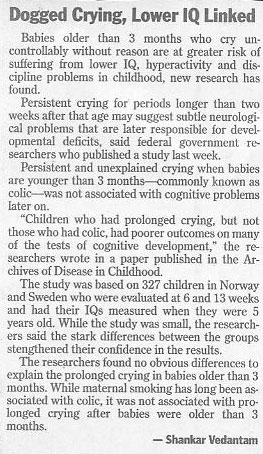
\includegraphics[scale=0.50]{../images/scientificReasoning2.jpg}
\end{center}
 \caption{ ~\citep{Vedantam:2004tz}}
\label{fig: scientificreasoningexample}
\end{marginfigure}

This section is written for the contemporary reader, not the ‘character’ you’ll be playing. The standards of what makes a good experiment have not changed significantly since the mid 1970s, so there should be no historical anachronisms contained herein.\footnote{Parts of this section is based on work completed during my Post-Doc at Washington University in St. Louis 2002--2004, in collaboration with William Bechtel, Adele Abrahamson and Carl Craver.}

F igure \ref{fig: scientificreasoningexample}) is a clipping from the Washington Post published in 2004. It’s one of these succinct summations of scientific research that appear all the time in the media---there is even a website (http:\slash \slash kill-or-cure.herokuapp.com\slash ) that tracks all the things that the British Tabloid \emph{The Daily Mail} has said either causes or cures cancer.

So what, exactly, is the claim being made here? What evidence is given in support of that claim? If we take the main headline

\begin{quote}

Dogged crying and lower IQs are linked
\end{quote}

as the central claim---the conclusion, as it were,---of the study that was performed, what would count as evidence in support? Against? 

What, exactly, does it mean to be `linked' anyway? How are they linked? Does increasing one cause increases in the other?

Fortunately, we have the original journal article for this one available, so I’ll quote the abstract:
\begin{apatextbox}{Abstract from  ~\citep{Rao:2004ku} }
\textbf{BACKGROUND:}

Long term studies of cognitive development and colic have not differentiated between typical colic and prolonged crying.

\textbf{OBJECTIVE:}

To evaluate whether colic and excessive crying that persists beyond 3 months is associated with adverse cognitive development.

\textbf{DESIGN:}

Prospective cohort study. A sample of 561 women was enrolled in the second trimester of pregnancy. Colic and prolonged crying were based on crying behaviour assessed at 6 and 13 weeks. Children's intelligence, motor abilities, and behaviour were measured at 5 years (n = 327). Known risk factors for cognitive impairment were ascertained prenatally, after birth, at 6 and 13 weeks, at 6, 9, and 13 months, and at 5 years of age.

\textbf{RESULTS:}

Children with prolonged crying (but not those with colic only) had an adjusted mean IQ that was 9 points lower than the control group. Their performance and verbal IQ scores were 9.2 and 6.7 points lower than the control group, respectively. The prolonged crying group also had significantly poorer fine motor abilities compared with the control group. Colic had no effect on cognitive development.

\textbf{CONCLUSIONS:}

Excessive, uncontrolled crying that persists beyond 3 months of age in infants without other signs of neurological damage may be a marker for cognitive deficits during childhood. Such infants need to be examined and followed up more intensively.
\end{apatextbox}

While the journalist\footnote{The journalist in question here is Shakar Vendantam, who went on to host the “Hidden Brain” podcast on NPR.} used the word ‘linked,’ the scientific paper makes slightly different claim: that crying “may be a marker” for cognitive deficits during childhood. This word change---from ‘marker’ to ‘link’---has implications that demand investigation.

The former claim---that ‘dogged crying’ \emph{is linked} to lower IQ---suggests a causal claim: that if you could just stop the child from crying, the child’s IQ would remain normal. The second---that crying \emph{may be a marker}---suggests that crying is an early sign of an underlying problem that manifests as lower IQ at a later date. The first implies one-way a causal relationship, the second, that both are caused by an underlying problem.

\newthought{The process of drawing upon information,} whether acquired through simple observation or through experiment, to answer questions is the crux of the activity of scientific reasoning. The answers to these questions are what scientists refer to as \emph{hypotheses}.\marginnote{A ‘hypothesis’ is often defined as an 'educated guess'. This overly-simple definition is really only suitable as a starting point. A hypothesis is a conjecture about the way some phenomenon in the world is or behaves. It might be about the origin of the universe, or the mechanisms of memory, but in either case, the hypothesis claims that something is a certain way. If we discover that the thing is not the way the hypothesis claimed, we have disconfirmed the hypothesis.} In a scientific investigation, one tests and rejects various hypotheses. 

Look back at the ‘Dogged crying’ abstract. You should note that this is study \textbf{not} an experiment. The authors of the study did \textbf{nothing} other than observe: they made no interventions to the babies or the mothers. They merely separated them into two groups, and measured those groups 5 years later. 

\subsection{The Paradigmatic experiments}
\label{theparadigmaticexperiments}

\newthought{The ‘Junior high’ version} of the scientific method tells us that to be science, one must observe-hypothesis-experiment-repeat. This simply isn’t true. Science uses a number of different methods, and not everything takes the form of the the classic \emph{experimentum crucis} that we were taught in seventh grade.
\begin{marginfigure}
 \begin{center}
     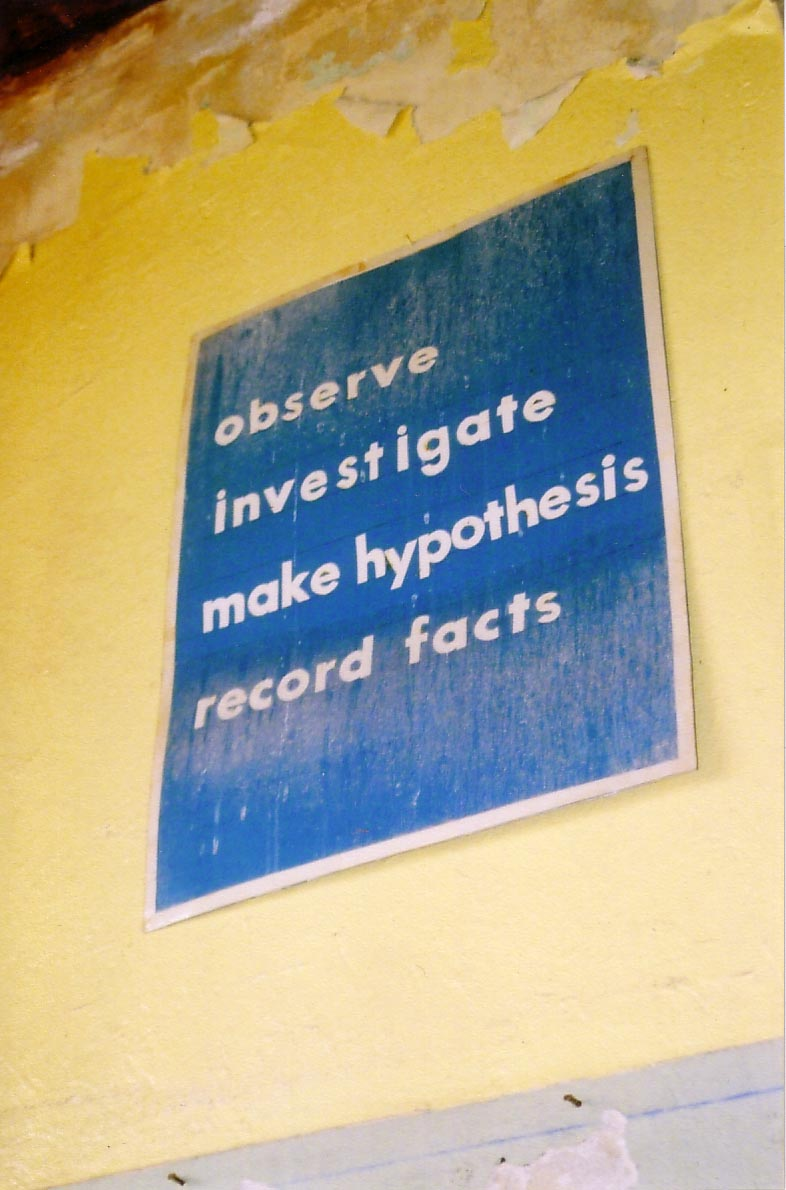
\includegraphics[scale=0.75]{../images/observe_poster.jpg}
\end{center}
 \caption{Photo of poster in abandoned junior high school in Hampstead, Maryland. Photo by Kenny Ditto, former student, 2008. Used with permission.}
\label{fig: scientificmethod}
\end{marginfigure}


Constructing good hypotheses and good questions to test hypothesis can be challenging, especially in psychology and psychiatry. In this section, we’ll introduce some basic terminology regarding scientific reasoning and discuss a few model studies---those we call ‘paradigms’---that have influenced how science has progressed.

\paragraph{The first paradigm: Newton’s \emph{experimentum crucis}}
\label{thefirstparadigm:newton’sexperimentumcrucis}

The concept of an ‘experiment’ in science is actually relatively new. 

As you may remember from \fullref{pre-historyofpsychology:empiricismaboutthemind}, we attribute the birth of the scientific method to Francis Bacon. His study of heat in the \emph{Novum Organon} established a model of scientific reasoning: first, draw axioms from experience; and second, deduce or derive new experiences from those axioms ~\citep[Bk. II, \S X]{Bacon:1620ui}

\begin{enumerate}
\item Catalog all the instances of the thing (“Table of existence and presence”, \S XI)

\item Catalog all the instances of things similar to the items listed in (1), but lacking heat (“Table of Absence”, \S XI)

\item Catalog all the instances of things that do not have heat but could (“Table of degrees or comparative instances”, \S XIII)

\item Finally, catalog all the instances of things that heat cannot be (“Table of exclusions”, \S XVIII)

\end{enumerate}

Only after these tables are made are we able to make a ‘First Harvest’, a first attempt to generalize across all these tables and interpret nature. Once this is complete, Bacon suggests we create tables of ‘privileged instances’--27 in total, that specify all instances that are solitary, revealing, concealed, etc. The 14th table is a table of ‘crucial’ or ‘critical’ instances.

\begin{quote}

We take the term from the \emph{signposts} which are erected at forks in the road to indicate amen mark where the different roads go. We have also chosen to call them \emph{decisive instances} and \emph{instances of verdicts}, and in some cases \emph{oracular} and \emph{commanding instances}. 
\end{quote}

This is where the term \emph{experimentum crucis} comes from, although for Bacon, it was a critical \emph{instance} of observation, not a critical experiment. Robert Hooke, who we now remember for ‘Hooke’s Law’ of springs, was the first to suggest that critical instances could be manufactured in a laboratory, and hence, become \emph{experiments}.

\begin{figure*}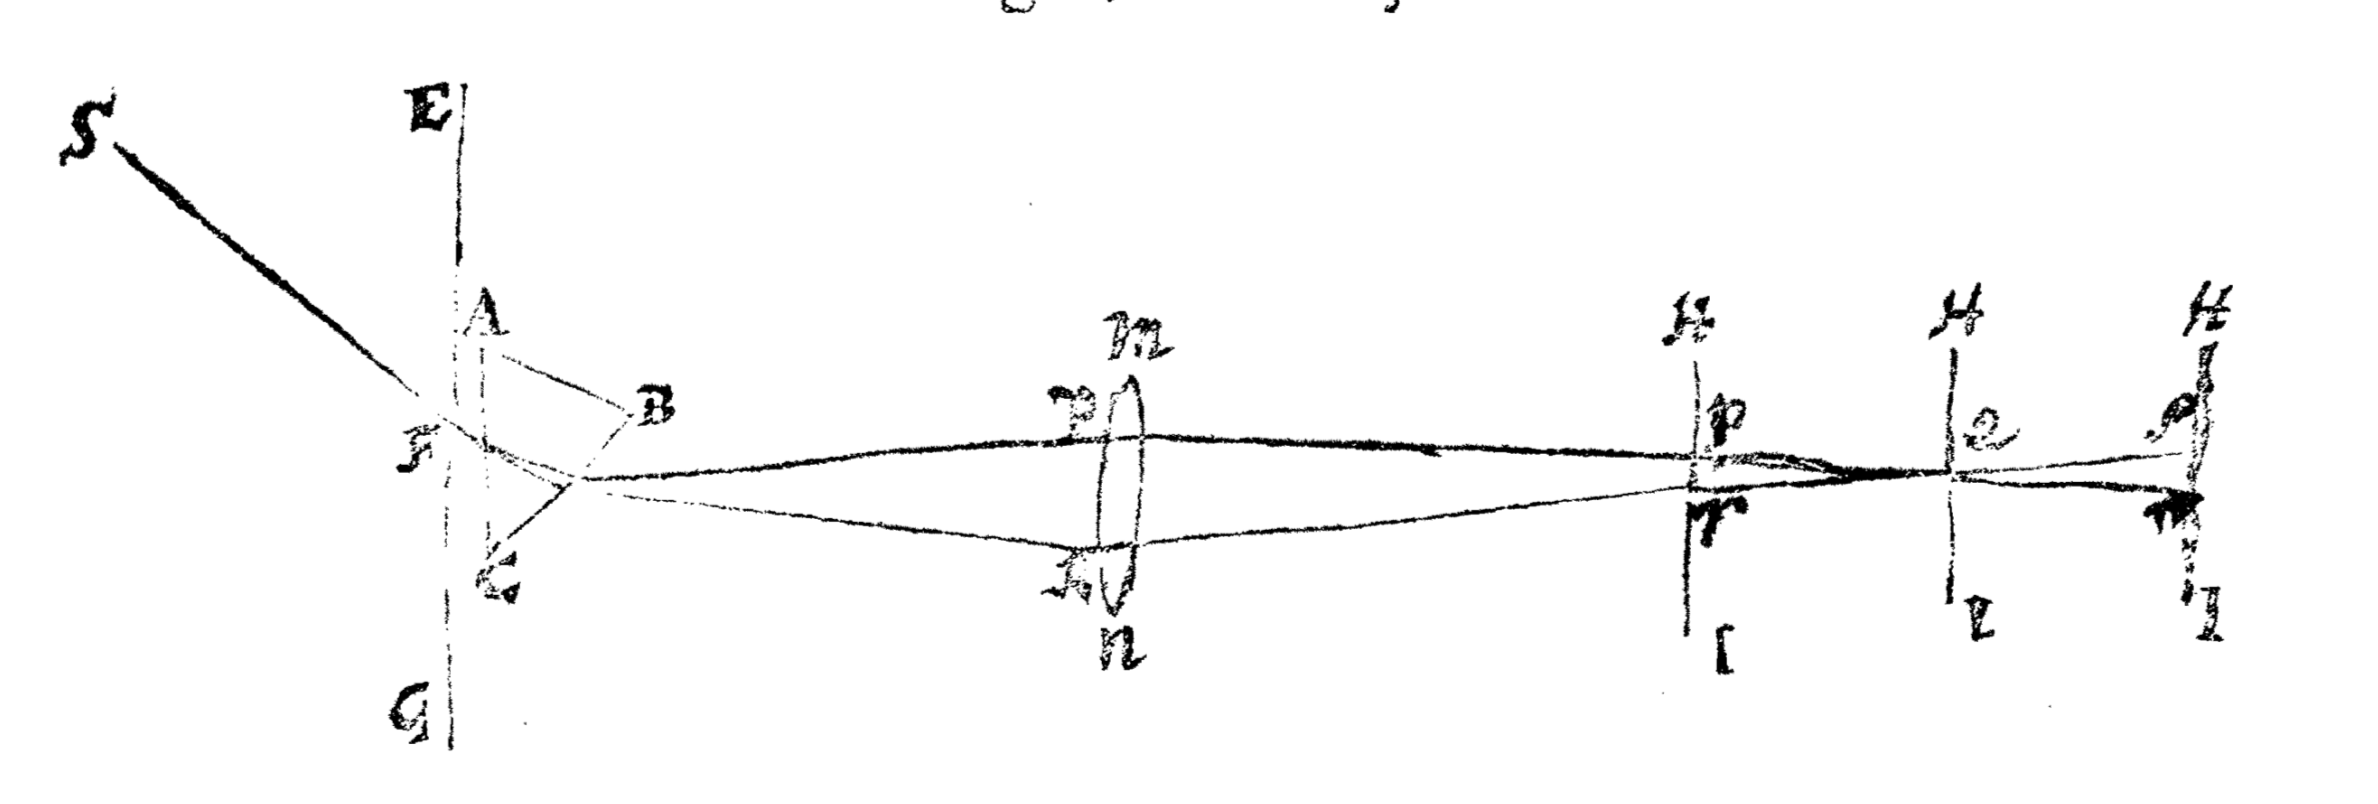
\includegraphics{../images/newton1671.png}\caption{Illustration of Newton's experiment contained in the 1st letter to the Royal Society, 1671}\label{fig:newton1671}\end{figure*}

Newton first started his experiments on light and prisms in the early 1670’s, reporting his initial findings to the Royal Society in 1671. ~\citep{Newton:1671uw} It is actually his \emph{second} letter on this topic, published in 1672, that is most frequently cited as the primary source. ~\citep{Newton:1672tm}. 

It is notable that Newton himself does not use the term \emph{experimentum crucis} in his original presentations of his experiments to the Royal Society in two letters in 1671 and 1672. In 1672--1673, Hooke viciously attacked Newton’s work. In 1673, Newton was a young man of 30, working primarily in Cambridge, not London. Hooke was 10 years his senior, an original member of the Royal society and well ensconced in the power structures of London.

But Hooke had a theory of light, was well known to be ‘irascible’, and did not appreciate new-comers. Newton responded in 1672 ~\citep{Newton:1672wd}, and again in 1673 ~\citep{Newton:1673tf}. But even in these, he does not call his experiments ‘crucial’. He only uses that term in his \emph{Opticks}, written 30 years later and published a year \emph{after} Hooke’s death. ~\citep{Newton:2018th}

I mention this because, as most students familiar with Reacting will understand, the \emph{actual} history is far more complicated than the digested version we get in most textbooks. The story Newton tells in the \emph{Opticks} of conceiving of and performing a \emph{crucial experiment} deduced by pure logic from the Bacon’s tables of induction is nothing more than a post-hoc myth.

But like Franklin’s kite, it is the myth, and not the actual history, that matters in understanding Newton’s influence on the development of science. So what did Newton show, and why was it ‘crucial’?

\newthought{The fact that white light} that passes through a prism refracts and takes on the colors of the rainbow was well understood in 1670. What was not understood was whether the colors of the rainbow were existent in the light and ‘revealed’ by the prism, or whether they were in the prism and ‘added’ to the white light as it passed through. In short, is the prism breaking light up, or is it acting as a colored filter?

Roughly, Hooke held the second: that light itself does not contain color, but it took on colors as it was ‘corrupted’ by the prism. Newton, on the other hand, thought that the light’s color and the angle of refraction were one and the same, and hence, the colors were contained in the white itself, and were only revealed by refraction through the prism.

A ‘crucial’ experiment must act like a signpost. It must distinguish absolutely between the two competing theories---like a fork in the road, at a critical experiment, the two theories diverge and cannot be recombined.
\begin{figure*}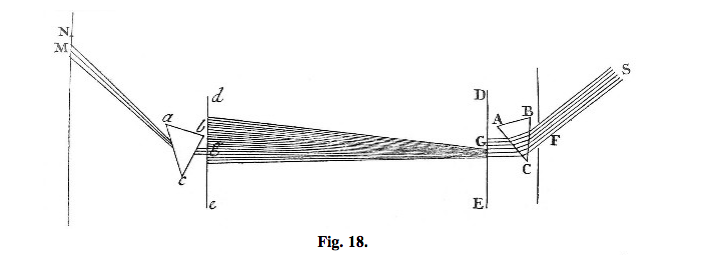
\includegraphics{../images/newton1704.png}\caption{Illustration of Newton's experiment contained in the \emph{Opticks}, 1704. Notice that the sun is on the right, and the rays move right to left, unlike the first from 1671.}\label{fig:newton1704}\end{figure*}

Newton and Hooke both predict that light passing through a prism will refract at a distinct angle, and will take on the colors of the rainbow. What Newton needs is a case in which Hooke predicts one thing, and he the opposite. 

So he sets up the experiment as designed in \ref{fig:newton1704}. Newton darkens the room, and opens a small pinhole in a sheet (F) covering the window. The light starts at (S), enters the room through the (F) and passes through prism (ABC). It then falls on sheet (DE), which has a hole (G). The light coming through G is a single color. It then passes through \emph{another} screen and prism. The resultant angle is measured. Newton observes, at least in 1672:

\begin{quote}

“And I saw by variation of those places that the light, tending to that end of the image toward which the refraction of the first prism was made, did in the second prism suffer a refraction considerably greater than the light tending to the other end.  And so the true cause of the length of that image was detected to be no other than that light consists of rays differently refrangible, which, without any respect to a difference in their incidence were , according to their degrees of refrangibility, transmitted to divers parts of the wall.”
\end{quote}

When light passes through the second prism, it is further refracted, but not changed in color\footnote{Newton himself describes the logic of his \emph{experimentum crucis} like this:

\begin{quote}

To determine by Experiments these and such like Queries which involve the propounded theory, seems the most proper and direct way to a conclusion. And therefore I could with all objects were suspended, taken from Hypotheses or any other heads other than these two; of showing the insufficiency of Experiments to determine these Queries or prove any other parts of my theory, but assigning the flaws ad defects in my conclusions drawn from them; or of producing other Experiments which directly contradict me, if any such may seem to occur. For if the Experiments, which I urge, be defective, it cannot e difficult to show the defects. But if value, then by proving the theory they must render all Objections invalid. ~\citep[p. 5005]{Newton:1672tm}
\end{quote}}. So how does this observation for a fork-in-the-road between his view and Hooke’s? That’s a subject of debate. But here’s my best take at his reasoning:

\begin{apatextbox}{Newton’s Experimentum Crucis} 

\begin{enumerate}
\item Either the colors and their respective angles are in the light itself, and the prism uncovers this fact, or the prism adds the colors and the angles by corrupting the pure white light.

\item If the former, then light passing through a second prism would (a) not change the color (for a color once revealed can’t be revealed again) BUT it would (b) double the angle on the second pass.

\item If the later, the light passing through a second prism would (a) change the color (for the prism adds color to whatever light it touches) AND it would (b) double the angle on the second pass.

\item Passing light through 2 prisms produces the same color as passing light through 1 prism (as well as doubles the angle).

\item Therefore, the colors and their angles are in the light itself 

\end{enumerate}

\end{apatextbox}

This experiment---and this reasoning---comes to be \emph{the} standard for a good experimental design. It is the ‘paradigmatic’ experiment of its era, the ‘paradigm’ of good science.\footnote{In contemporary academic English, the word ‘paradigm’ is used to mean, roughly ‘word-view’. That usage descends from this use of the term, as the modern use can be traced back to Thomas Kuhn’s \emph{Structure of Scienctific revolutions} (~\citep{Kuhn:1996fi}). In it, he describes scientific progress as changing eras in which scientists look to a particular experiment as the best model of scientific reasoning, and seek to replicate that experiment in their own work. That experiment is the ‘paradigm’ for that era of scientific inquiry. Over time, people started using the word ‘paradigm’ to refer to the era, and the people in it, rather than the experiment they valued.} 

\paragraph{The paradigm in experimental psychology: Hermann Ebbinghaus}
\label{theparadigminexperimentalpsychology:hermannebbinghaus}

As you may recall from \ref{birthofpsychology:germanphysiologicalpsychologyinthe1880s-1890s.}, in the 1860s and 1870s a handful of researchers in German started applying the experimental method to sensation and perception. Fechner’s law was one of the first great successes of this era, as for the first time, it related a physical phenomenon to a psychological one with the precision of mathematics. 

Today, Ebbinghaus is frequently characterized as the ‘founder’ of experimental psychology---as he site ‘encyclopedia.com’ does---and his experiments frequently taught in intro to research methods courses. This makes his work a ‘paradigm’ for contemporary psychology. In order to understand what counts as ‘good science’ in this environment, we must understand Ebbinghaus.

The first step in scientific endeavor into a new domain, according to Ebbinghaus, is to 

\begin{quote}

The method of obtaining exact measurements i.e., numerically exact ones of the inner structure of causal relations is, by virtue of its nature, of general validity. This method, indeed, has been so exclusively used and so fully worked out by the natural sciences that, as a rule, it is defined as something peculiar to them, as the method of natural science. ~\citep[p. 7]{Ebbinghaus:1885ud}
\end{quote}

\begin{marginfigure}
 \begin{center}

     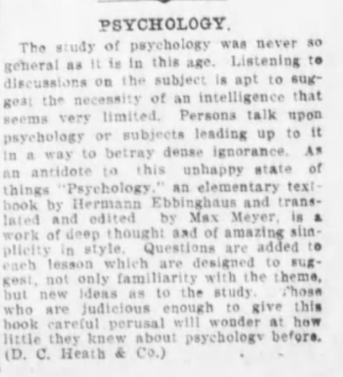
\includegraphics{../images/ebbinghaus-clip.png}
\end{center}
 \caption{Notice of Ebbinghaus’ book “Psychology”, from the Brooklyn Daily Eagle, Dec 19, 1908}
\label{fig: ebbinghaus-clip}
\end{marginfigure}


Following Fechner, the primary goal of scientific investigation---prehaps \emph{the} defining feature of science itself---is the creation of mathematically precise descriptions of natural phenomena. 

When Ebbinghaus first approached the question of memory, he needed to create an environment, like Newton’s darkened room, where comparisons between different tasks could be compared. 

The first step is to control “the mass of conditions which have proven themselves causally connected with a certain result”, then, one of those is systematically varied, and the resulting effect measured.

\newthought{Ebbinghaus set out to systematically measure memory}---so he created a protocol for testing his own memory. In order to control his own personal associations with words, which might make them more memorable, he created a list of 2,300 1-syllable nonsense words. These were drawn randomly for each experiment. He then memorized lists and he measured how many he could remember after a given time period---he didn’t do this by introspection, but forced himself to actually write down all that he could recall, and check to see how accurate he was. He formalized the process of memorization, going so far as to use a clockwork mechanism to ensure that he spent the exact same amount of time memorizing each list.

There were things he could not control, of course. He recognized that his own accent and ‘mother-tongue’ might influence the test, the ‘conditions of his daily life’ might have an impact---he recognizes that his mind is typically fresher in the morning than the evening, for example. The experiments took months to complete, and there could be seasonal effects. 

He then varied the length of the lists and compared it against the time it takes to memorize. And he did this repeatedly, recording 518 lists over two periods, 1789--1790 and 1883--1884.
\begin{figure*}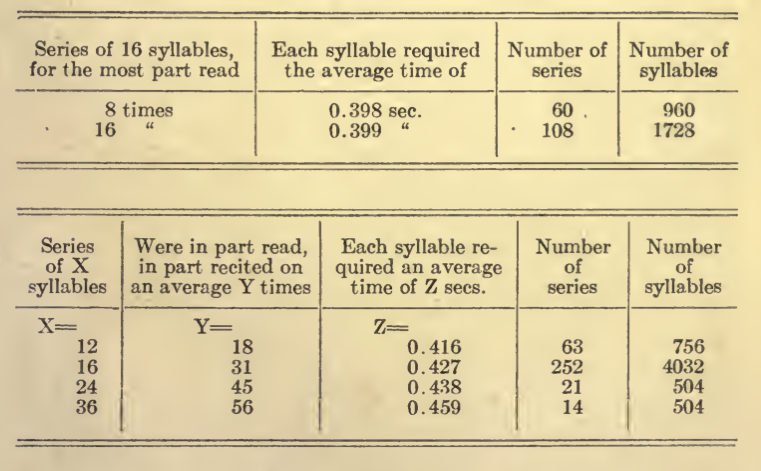
\includegraphics{../images/ebbinghaus1885.png}\caption{Ebbinghaus’ first table of results in his \emph{Memory}, 1885}\label{fig:ebbinghaus1}\end{figure*}

He also counted, using a string of beads, the number of repetitions it took to memorize a list. This produced, after many variations and trials, the chart to the right, not called ‘The learning curve’.
\begin{marginfigure}
 \begin{center}

     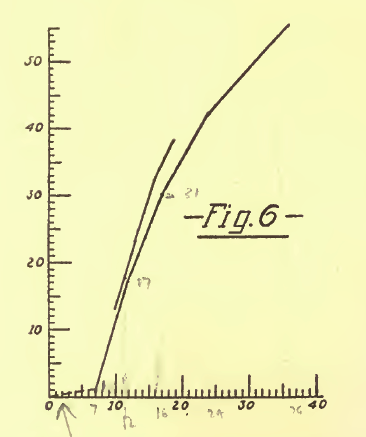
\includegraphics[scale=0.5]{../images/ebbinghausFig6.png}
\end{center}
 \caption{Screenshot of “Fig 6” from p. 48, Ebbinghaus 1885. Now called ‘the learning curve.’}
\label{fig: ebbinghaus6}
\end{marginfigure}


\newthought{Ebbinghaus then turned his attention to recall and retention.} Working from the commonsense notion that the longer you study, the longer it is retained, Ebbinghaus designed a protocol whereby he would measure the number of repetitions it would aka not re-learn a list after a given amount of time. Perfect recall would ’cost’ no further repetitions or time. Total failure would (presumably) require the same amount of time as it took in the first place.

As before, this protocol is designed to create a numeric representation (number of repetitions) of a psychological idea (ability to recall). As one might expect, the higher the number of repetitions on learning, the fewer needed after 24 hours to recall the list perfectly.

Measuring in seconds, Ebbinghaus determined the amount of time ‘saved’ when re-learning by repeating the learning in the first place---and the average number of seconds saved by each additional repetition. His results are remarkable:
\begin{marginfigure}
 \begin{center}

     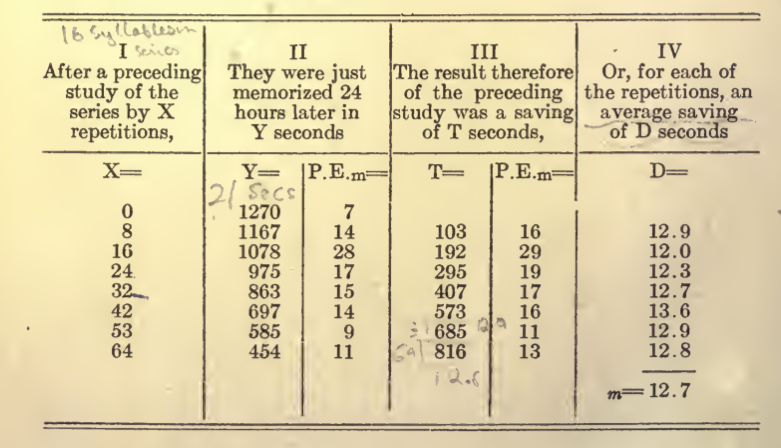
\includegraphics[scale=0.5]{../images/ebbinghaus2.png}
\end{center}
 \caption{Screenshot recall table, p. 56 Ebbinghaus 1885.}
\label{fig: ebbinghaus2}
\end{marginfigure}


\newthought{His last great contribution to psychology is the ‘forgetting curve’.} Using the measurements developed in previous experiments, Ebbinghaus started measuring the number of repetitions needed to restore a list versus the amount of time since the list was memorized. He found that after just and hour, 1\slash 2 of the original work was required to refresh the list. But after 8 hours, it was only 2\slash 3rds, not the whole amount. He also discovered that individual items in the list are retained differently according to their serial position. He summarized his findings as:

\begin{quote}

The strength of the connection, and therefore the amount of work which is eventually saved, is a decreasing function of the time or of the number of intervening members which separated the syllables in question from one another in the original series. It is a maximum for immediately successive members. The precise character of the function is unknown except that it decreases at first quickly and then gradually very slowly with the increasing distance of the terms. ~\citep[p. 107]{Ebbinghaus:1885ud}
\end{quote}

While the list of psychological principles attributed to Ebbinghaus is long, it is absolutely true that he noted what is now called the “magic number 7”--that the longest list of random syllables one can remember without practice is 7.\footnote{George Miller will be presenting his update to this famous result ‘The Magic Number Seven plus or minus 2’ at the first conference.} ~\citep[p. 47]{Ebbinghaus:1885ud}

It’s also true that all of these experiments were preformed on an experimental group of one individual: himself. There was no control group and no random sampling of a population. But it is also noteworthy that he recognized these limitations in his study: 

\begin{quote}

The tests were all made upon myself and have primarily only individual significance. Naturally they will not reflect exclusively mere idiosyncrasies of my mental organisation; if the absolute values found are throughout only individual, yet many a relation of general validity will be found in the relation of these numbers to each other or in the relations of the relations. ~\citep[Author’s preface, p. v]{Ebbinghaus:1885ud}
\end{quote}

Ebbinghaus’ paradigm is not having a control group, blinding reviewers, or randomizing across a population. Rather, I suspect, Ebbinghaus’ paradigm comes down to two things:

\begin{enumerate}
\item Ebbinghaus’ goal throughout these studies was to describe psychological phenomena in the precise language of mathematics. While \emph{Memory} does contain a few formulae, the whole of the book is consumed with the validity of his measurements of the time it takes to memorize and the costs of forgetting.

\item Ebbinghaus set a standard for transparency of data and thoroughness in controlling potential confounding variables. He addresses every potential confound as it arrises and redesigns his protocol to control, or measure that confound. And those he cannot, he labels and presents to the reader. The passage quoted above demonstrates his laudable self-reflection, precisely specifying the weakness in his experiment that he could not control.

\end{enumerate}

Indeed, in reading \emph{Memory}, one cannot help but be impressed by Ebbinghaus’ thoroughness and dedication to the transparency of his research. The book is only 117 pages of text, yet it covers 5 years of experimentation and thousands of trials. This, I suspect, is the true paradigm of Ebbinghaus: that psychological measurement must be carried out extraordinarily carefully, with all due attention to potential confounds.

\subsection{Varieties of Scientific Inquiry}
\label{varietiesofscientificinquiry}

Most scientific studies seek to establish that two (or more) variables are correlated. To say that two variables are correlated is to say, at first pass, that you can predict the value of one given the value of the other. The degree to which your prediction is reliable is the correlation coefficient: a value of 1 means that you can precisely and accurately predict one of the values from the other. \begin{thesis}[Correlation]Two variables are correlated if you can predict the value of one given the value of the other.\end{thesis}

A value of 0 means that any prediction you make would be random in nature. A positive correlation means that as one variable increases, so does the other, and a negative correlation means that as one variable increases, the other decreases. 

There are two basic studies that seek to establish a correlation:

\begin{itemize}
\item Non-Intervention, i.e. ‘Observational studies’

\item Intervention, i.e. ‘Experimentation’

\end{itemize}

Another important aspect of scientific inquiry is modeling, where a scientist seeks to \emph{explain} a correlation by positing a mechanism that behaves in the same way in the same conditions. To understand the importance of---and the limitations to---modeling, we’ll need to first understand the logic of scientific inquiry as well as the potential and limitations of both observational and experimental research.

\subsubsection{The Logic of evidence}
\label{thelogicofevidence}

\paragraph{The hypothetico-deductive method}
\label{thehypothetico-deductivemethod}

Some have characterized the testing of hypotheses in science as a two-step process. The first step of the argument involves the deduction of a prediction from the hypothesis to be tested. Then, after we see whether the prediction turns out to be true, we can draw conclusions about the truth of the hypothesis. If the prediction turns out to be true, the hypothesis has been confirmed. The argument might run roughly as follows:
\begin{apatextbox}{Affirming the consequent}
If Hypothesis, then Prediction.\\
The Prediction is true. \\ \hline
Therefore the hypothesis is true.
\end{apatextbox}
If the prediction turns out to be false, the hypothesis has been falsified. The argument might be put roughly as follows:
\begin{apatextbox}{Modus Tollens / Denying the consequent}
If Hypothesis, then Prediction.\\
The Prediction is not true.\\ \hline
Therefore, the Hypothesis is not true.
\end{apatextbox}
Anyone who has taken Logic or Critical Thinking will notice an important difference between these two arguments. 

The first argument is invalid and the second is valid. 

In the first case, it is possible for the both of the premises\footnote{A ‘premise’ is a part of an argument that is asserted as reasoning for drawing the conclusion. In these two cases, there are two premises and one conclusion, which is separated by a single line. A \emph{valid} argument is one where it is impossible for the premises to be true and the conclusion false. In other words, a valid argument is one where if you agree with the premises, you \emph{must} agree with the conclusions.} to be true and for the conclusion to nonetheless be false. For example, I could argue `If you are not over 21, you cannot drink beer. I am not drinking beer, therefore, I am not over 21.' Both premises are true, but the conclusion is false. I am both over 21 and drinking coffee. The argument, therefore, does not \emph{guarantee} the truth of the conclusion, and therefore is not valid.

Let us take an example from the history of science: the positions of the planets can very easily be predicted with Ptolemy's 2nd Century geocentric model of the solar system, with Kepler's heliocentric geometrical model, or with Newton's gravitational theory. We now know that none of these are technically true descriptions of planetary motion (they all have well-known exceptions or make positively false claims); still each makes a number of true predictions. Each of them can make produce premises like `If my theory is true, then Venus will rise in the morning and in the evening', and `Venus rises in the morning and in the evening', but the joining these true premises into an argument can not ensure that the theory is true. In fact, none of them are.

The first argument is a fallacy\footnote{‘Fallacy’ is a word philosophers use for commonly-used arguments that do not guarantee truth. There is a long history of cataloging fallacies, and many lists can be found online. Knowing the name of a fallacy is less important than understanding \emph{why} they are fallacious: one could agree with all the premises, yet still disagree with the conclusion.} known as the ``affirming the consequent''. The second premise (the prediction) is the second term, or consequent, of the first premise (If hypothesis, then prediction). The argument states the first premise (If hypothesis then prediction) and then affirms its consequent (prediction), in order to conclude that the hypothesis is correct. 

Although arguments of this sort superficially resemble truth-preserving arguments like the second argument above, we have seen that it fails to ensure a true the conclusion when the premises are true. We will call these arguments - arguments that superficially resemble deductive arguments but are not truth-preserving - fallacies.

Not so for the second argument. If the hypothesis deductively entails an prediction and that prediction turns out to be false, then something \textbf{must} be wrong with the hypothesis. 

\newthought{The arguments above embody} what is known as the ``hypothetico-deductive'' model of scientific reasoning. The hypothesis entails, deductively, a prediction and the prediction is then checked against the world. If the prediction turns out to be true, the hypothesis is confirmed (though not with certainty). If it turns out to be false, the hypothesis is falsified with certainty. 

\newthought{This fact of logic}, that if the conclusion of a valid argument is false, at least one of its premises \emph{must} be, lead Philosopher Karl Popper to propose a definition of scientific methodology we call “falsificationism.” According to Popper, as the hypothetical-deductive’ model of science can never \emph{prove} anything, it is science’s responsibility to propose bold predictions that can be \emph{falsified}. Scientists seek to disprove theories, not to prove them. And a theory is well-supported when it cannot be---or has not been yet---falsified. Popper’s view is still widely held by scientists. \begin{marginfigure}
 \begin{center}
     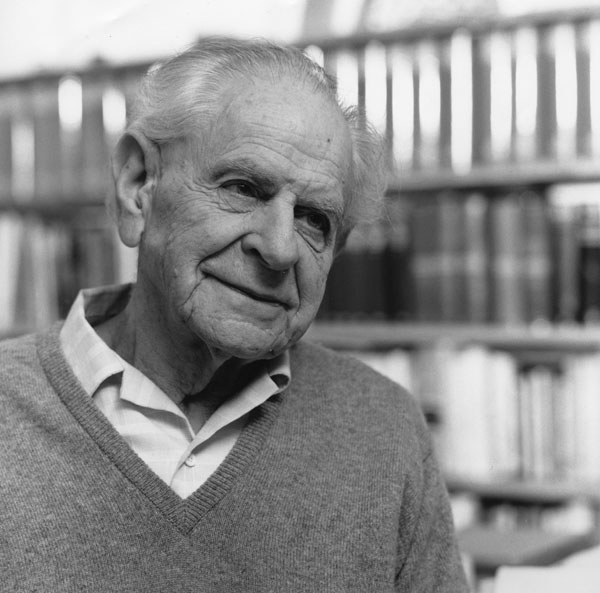
\includegraphics[scale=0.50]{../images/Karl_Popper2.jpg}
\end{center}
 \caption{Karl Popper, 1990, By Lucinda Douglas-Menzies  link [No restrictions], via Wikimedia Commons
}
\label{fig: karlpopper}
\end{marginfigure} 

\newthought{There is one more complexity} to the simple hypothetico-deductive method that ought to be mentioned explicitly. Typically, the hypothesis and observed data require additional auxiliary hypotheses to entail the prediction. Suppose that we wanted to test the hypothesis about conservation of momentum. And suppose that we started balls of known momenta at known velocities and then measured their velocities after the collision. In order to know what to predict, we would have to trust our methods for moving the balls at the said velocity, and we would have to trust our techniques for measuring their velocities after the collisions. Our prediction might fail because our instruments aren’t working rather than because the hypothesis is wrong. So we need to add explicitly some assumptions about the techniques used to measure a phenomenon.\begin{thesis}[Auxiliary Hypothesis]\label{thesis:auxiliaryhypothesis}
An \emph{auxiliary hypothesis} is a hypothesis about the methods, techniques, materials, or instruments used in an experiment that ensures the formulation of a prediction from a hypothesis.\end{thesis}

These assumptions — for example, that our techniques for measuring velocity are accurate — comprise the \emph{auxiliary hypotheses} that inform our prediction. There are always a number of auxiliary hypotheses informing every prediction. In some ways, a given prediction is just one part of a web of hypotheses that come into play in a given theory.

\subsection{Observational research}
\label{observationalresearch}

We acquire knowledge of the world primarily through our senses. As humans, we rely most heavily, but clearly not exclusively, on vision. Seeing the world seems very straight-forward. We open our eyes and the world impresses itself upon our consciousness.
\begin{marginfigure}
 \begin{center}


     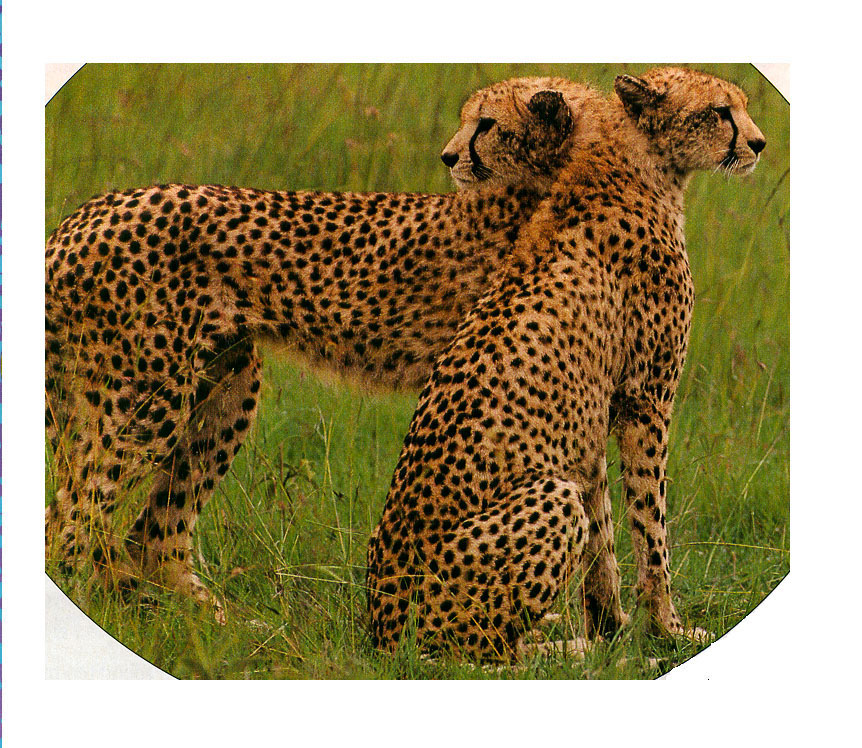
\includegraphics[scale=0.50]{../images/AmbigCheeta.jpg}
\end{center}
 \caption{Ambiguous Cheetahs, from  ~\citep{Pitts:2007km}}
\label{fig: ambiguouscheetahs}
\end{marginfigure}

Take a look at the image to the right. Which head goes with which cheetah? Can you flip your interpretation to see it the ‘other way’? There are \emph{tons} of created images like this, from the Necker cube to Salvador Dali paintings, the way you see the image can change dramatically, depending on the environmental conditions or what you had experienced just before seeing the image.

Our ability to see is, in part, learned. One aspect of `successful' seeing is the ability to recognize things when one encounters them again. Recognition requires the ability to categorize. Seeing, in this robust sense, also implies the ability to organize the categories into a taxonomy or classification system.

Although much scientific research goes beyond mere observation to posit causal processes and mechanisms behind what is observed, observational research plays a vital role in the development of scientific knowledge— both in delineating the phenomenon of study and in validating hypothesis and predictions. When conducting observational research, the question of how we organize observations into categories, as well as how we organize categories into taxonomies, plays a central role. In addition, we must pay careful attention to the notion of a `variable', and how we measure and estimate the values of variables.

Observational research is an important part of the scientific toolkit. Here we’ll present two paradigmatic observational studies that were hugely influential in the 1970s.

\subsubsection{Margaret Mead}
\label{margaretmead}

Margaret Mead was an extraordinarily talented student at Barnard college, completing here Bachelors in 1924. She earned her Masters’ under the supervision of the famous Anthropologist Franz Boas a year later in 1925. In 1926, at the age of 23, she set off for nine months on the Manu’an Islands of American Samoa. 

She was inspired in the trip by Boas, and his concern that problems in the mental life of adolescents, was the result of western culture---specifically our prohibitions on sex---not any individual dysfunction. 

But how can one test such a hypothesis? One cannot, because of basic human ethics, separate a bunch of children at birth to raise them outside of western culture. Nor would it be helpful to find groups of children in western culture and follow them, because there are two many variables at play to isolate the influence of sexual repression on mental health. As she argues:

\begin{quote}

The only method is that of the anthropologist, to go to a different civilization and make a study of human beings under different cultural conditions in some other part of the world. For such studies the anthropologist chooses quite simple peoples, primitive peoples, whose society has never attained the complexity of our own. 
\end{quote}

This last point is important: the anthropologist has to become ‘embedded’ int the culture to understand it enough to communicate with its people on their terms. Western societies, even those sometimes found on the outskirts, are simply too complex to allow a quick study. Their language alone would take years to master, and their social structures too complex to understand quickly.\footnote{I hope the reader recognizes that I am speaking here as Mead did, and as one would in the 1970s’. I don’t believe a word of this, as you might expect. To contemporary thinking, Mead’s presumption of simplicity of the Somoan culture and language is the core failing of her study.} As “she could hope for great intimacy in working with girls rather than with boys”, ~\citep[p. 9]{Mead:1928uk} she choose to study adolescent girls in Samoa.

As her professor Boas writes in the preface to \emph{Coming of Age in Samoa}, 

\begin{quote}

In our own civilization, the individual is beset with difficulties which we are likely to ascribe to fundamental human traits. When we speak about the difficulties of childhood and of adolescence, we are thinking of them as unavoidable periods of adjustment through which everyone has to pass. The whole psycho-analytic approach is largely based on this supposition.
The anthropologist doubts the correctness of these views, but up to this time hardly any one has taken pains to identify himself sufficiently with a primitive population to obtain an insight into these problems. We fell, therefore, grateful to Miss Mead for having undertaken to identify herself so completely with Samoan youth that she gives us a lucid and clear picture of the joys and difficulties encountered by the young individual in a culture so entirely different from our own. ~\citep{Mead:1928uk}
\end{quote}

Mead describes society which has very different sexual mores: 

\begin{quote}

“Masturbation is an all but universal hair, beginning at the age of six or seven. There were only three little girls in my group ho did not masturbate{\ldots} Boys masturbate in groups but among little girls it is a more individualistic, secretive practice.” ~\citep[p. 136]{Mead:1928uk} 
\end{quote}

The girls, she writes “deter marriage through as many years of casual love-making as possible” ~\citep[p. 195]{Mead:1928uk}

And as a result, there are few conflicts or troubles in the mental life of adolescent girls. Thus, adolescence is not a difficult time period for \emph{all} girls. As it is a major problem in the west, it must then follow that the ‘storm and stress’ of girls’ adolescence is due to the culture they inhabit, not their biology or process of maturation.

\subsubsection{Roger Brown}
\label{rogerbrown}

Roger Brown and his research team at Harvard University in the 1960s visited the homes of “Adam,” “Eve,” and “Sarah” every two weeks during the period they were first acquiring English. The team audiotaped and transcribed everything the children and their mothers said, resulting in three corpora of such high quality that they are still in use. (Although teenagers talk somewhat differently today than in the 1960s, 2-year-olds then and now talk about juice, dogs, hats, more, allgone, etc.) 

Especially in the earliest stages, children omit a lot and parents sometimes fill in what is missing. Here is one of Brown’s examples:

\begin{apatextbox}{Brown’s first example}
Child- Throw Daddy \\
Mother- Throw it to Daddy
\end{apatextbox}

The grammars that Brown’s group wrote to account for such simplified language were far more complex than you might imagine. Even more intriguing, though, were child utterances that had to be changed, not just expanded, to get an adult utterance. For example:

\begin{apatextbox}{Brown’s second example}
Child- What John will read? \\
Mother- What will John read? 
\end{apatextbox}~\citep{Brown:1968df}

Notice that there is \emph{no} attempt by the researchers to intervene in these situations. Parents are not coached to speak to their children in a certain way, nor were they asked to fill in the sentences or avoid making corrections. There is no ‘control’ group, no independent variables, no dependent variables. Brown and his colleagues are simply observing speech of children as it occurs.

An understanding of how children acquire language begins with extensive observation and careful records, focused especially on ages 1--3 years. The key product is a child language corpus, which is a written transcription of all utterances by a particular child and, usually, at least one adult who is present and interacting with the child during one or more periods of observation. As technology has progressed, researchers have gained choices. In the earliest studies (and still occasionally by choice today) observations were recorded in handwritten diaries (motion picture film and soundtracks existed but were not practical in this context). By the 1960s, audio recordings were made at the time of observation — sometimes supplemented by handwritten notes — and then transcribed into written form. 

So what are we observing here? At first pass, it may appear that the child just mixed up the word order a bit, and was corrected by a parent. Brown’s group proposed a much deeper analysis in terms of what would become know as a “generative grammar.”
\newthought{The earliest versions of generative grammar} emphasized the idea (adapted from Chomsky’s mentor, Zellig Harris) that a sentence should be viewed as the product of a series of transformations. Consider the following sentences:

\begin{apatextbox}{Generative Grammar}
\rowgroup{John will read what? BASE QUESTION (atypical word order for a question)} \\
\rowgroup{What John will read? PREPOSING TRANSFORMATION: moves wh-word (what) to the front.} \\
\rowgroup{What will John read? TRANSPOSING TRANSFORMATION: reverses the subject (\emph{John}) and the auxiliary verb (\emph{will}).}
\end{apatextbox}

The final form in the sequence is what an adult would typically say. The transformations and the intermediate form are not directly observed, but Chomsky claimed that they can be inferred and are part of the speaker’s linguistic competence.

\newthought{Brown and his colleagues suggested} that the child was in the process of acquiring transformations, and at this point (about 3 years of age) had acquired preposing but not transposing. As a result, the “hypothetical intermediate” became an actual, observed form. Not only did this give a neat explanation of what the child said, but in the other direction it lent support to Chomsky’s theory. ~\citep{Brown:1972to} ~\citep{Chomsky:1965uu}

\subsubsection{What all observational research has in common}
\label{whatallobservationalresearchhasincommon}

\begin{itemize}
\item Observational researchers always observe some type of phenomena. (obviously)

\item Observational researchers make some sort of record and analyze data obtained from it.

\item Observational researchers do not manipulate variables.
Reasons to do observational research

\item Description (atheoretical research): To obtain a general characterization of the behavior of a particular individual or group in a specified domain and setting.

\item Exploratory research (pretheoretical research): To develop hypotheses and\slash or tentative theories. The researcher obtains a characterization of behavior, but with the goal not only of description but also of explanation.

\item Confirmation or falsification (theoretical research): To test hypotheses — which may come directly from exploratory research or have a more complex history. For example, a tested hypothesis may be obtained by revising a hypothesis that was suggested by exploratory research but failed to be confirmed. (Note: If the hypothesis concerns a causal claim, observation alone will not provide strong test; if possible, an experiment should be done.)
Two types of observational research

\item Naturalistic observation: unobtrusive, passive observation in a natural environment. It is important to minimize any impact of observer bias. For examples, the observers may be research assistants who are blind to the goals of the study.

\item Participant observation: the observer interacts with those being observed, typically within a natural environment or context. It is important to minimize reactivity — that is, the influence of the observer's presence on the behavior of those being observed. For example, a participant observer can seek to achieve some degree of unobtrusiveness and passivity by avoiding leadership roles and making written records when out of sight.

\end{itemize}

\newthought{Two of the major risks} of observational research are \emph{observer bias} and \emph{reactivity}.

As we noted earlier, when an individual expects something to happen, he or she is more likely to notice it. This gives rise to what is known as \emph{observer bias}. A classic example is provided by a study of college students observing flatworm behavior by ~\citep{Cordaro:2016bv}. Student observers were to record how many head turns and body contractions were made by two groups of flatworms. 

Although there were no differences between the two groups, the observers were led to believe group A would have higher rates of both turning over and contracting than group B. The observers ended up recording twice as many head turns and three times as many body contractions for group A. Since there was no reason to expect a large difference in the actual behaviors, the results appear to be due to the expectations of the observers. Such biasing is typically not deliberate — the observers may be trying to honestly report what they observer, but processes unknown to them are influencing their behavior.

Although observer bias cannot typically be eliminated, it can be moderated. One strategy is to use observers who have not been influenced by the expectation. Such observers are characterized as blind. Observers are said to be blind when they do not know why the observations are being performed or any hypotheses being entertained.

A second strategy is to employ multiple observers and evaluating the agreement between them. This is known as ‘inter-observer reliability, and is measured by Cohen’s Kappa. If observers are influenced by expectations to see more examples of particular behaviors in one group than in another, they are nonetheless likely to differ in which additional cases they detect or which they miss.

\subsection{Testing causal claims experimentally}
\label{testingcausalclaimsexperimentally}

In the ideal experiment, the only plausible explanation the two variable changing together is that they are causally connected. All other possible explanations—those based on the effects of other untested variables—have been ruled out by ‘controlling’ them. The simplest form of an experiment has:

\begin{itemize}
\item an independent variable—the suspected cause—is manipulated.
\begin{thesis}[Independent variable]
Independent variable (manipulated): a variable of interest that is suspected to have a causal impact on the dependent variable, and is manipulated in an experiment to put this to the test.\newline
The ‘independent variable is sometimes called the suspected cause, the IV-manipulated or manipulated IV, or just ‘IV’, if context makes clear that this is a manipulated IV, not a measured IV.
\end{thesis}

\item a dependent variable—the suspected effect—is carefully measured. \begin{thesis}[Dependent variable]
Dependent variable: a variable of interest that is suspected to be affected by the independent variable, and is measured in experimental or correlational tests of this hypothesis.
\newline
The ‘dependent variable’ is also sometimes called the ‘DV’, the suspected effect.
\end{thesis}

\item extraneous variables are controlled

\end{itemize}

If the independent variable is \emph{in fact} causally related to the dependent variable, then altering the value of the independent variable will produce changes in the value of the dependent variable. Moreover, these changes would not be found if the independent variable were not changed.

We will begin with the simplest case, one in which the causal relations are deterministic (that is, a change in the independent variable always produces the same change in the dependent variable). In such cases we sidestep the additional concerns with statistical analysis. But in later parts of this module we will consider such statistical relations as other factors that affect to validity of experimental demonstrations of causation.

\newthought{The core idea of an experiment} is that the researcher \emph{manipulates} the suspected cause and \emph{measures} the suspected effect. By contrast, a study in which the researcher \emph{measures} both the suspected cause and the suspected effect we call a “correlational study.” 

If this manipulation produces an change in the value of the variable suspected of depending on the causal variable, we have the strongest evidence we can get that the suspected relation is genuinely causal. If it does not produce the expected changes, any correlation previously noted between the variables may be due to the fact that they are both caused by a third variable. To determine the real cause, we would then need to figure which other variable is the best candidate and manipulate it in a new experiment — perhaps repeating this cycle more than once until we hit the right variable.
Recall that we already have some useful terminology to use when causal hypotheses get put to the test in a research study. The suspected effect is the \emph{dependent variable}. The suspected cause is the \emph{independent variable}, which can be further specified as manipulated (if the study is an experiment), or measured (if the study is correlational, in the broad sense of that term that can include comparing group means as well as computing correlation coefficients). Since we are focusing on experiments in this module, the following are definitions of independent variable (manipulated) and dependent variable given in the margin at the right.

Whenever you see the term independent variable used by itself, one must determine whether it is manipulated or measured. This will be important when you evaluate the outcome of the study and ask how well it supports the suspected causal connection.

The most basic experiments manipulate only one independent variable and are limited to two values of that variable. That is, the independent variable is treated as the simplest kind of categorical variable—a binary variable—even if it is based on a score variable. Dependent variables usually are score variables, but need not be; methods of analysis are available for DVs at any level of measurement, all the way down to binary. 

\newthought{More complicated experiments} may investigate multiple factors at the same time as well as multiple levels of the same factor. For example, if we were designing an experiment to examine the effects of both \emph{diet} and \emph{exercise} on \emph{weight-loss.} This would be a two-factor study. And rather than just using two levels, we might use four levels of the exercise factor—none, light, moderate, and heavy—and three levels of the diet factor—high-protein, high- carbohydrate, and balanced. Exercise is a rank variable here and diet is categorical. Usually the statistical analysis will treat both as categorical, which is fine. However, even if the result were statistically significant, it would be hard to interpret results for exercise in which none and moderate led to weight loss and light and heavy did not.

In choosing the levels of a factor, sometimes experience or common sense are very helpful in avoiding results that are inadequate for your purpose or difficult to interpret. For example, if your hypothesis is that eating oatmeal affects cholesterol levels, manipulating diet such that one group gets one teaspoon per month more oatmeal than the other group is unlikely to produce an effect. At the other extreme, manipulating diet such that one group gets no oatmeal and the other must eat 50 cups a day would make the second group overweight and unhealthy. It would be more reasonable to contrast no oatmeal to an easily sustainable amount of oatmeal (perhaps two servings per week of ¾-cup of oatmeal) to a larger, but not ridiculous, amount of oatmeal (perhaps one cup per day).

\newthought{Some predictions can be tested} by manipulating an independent variable once. What is required is that the relation between the independent and dependent variable be \emph{deterministic}. That is, each time the independent variable takes a particular value, its effect on the dependent variable should be the same. For example, replacing water with mercury in 100 vacuum tubes in a given place and time should have the same effect (a reduction in height from 34 feet for water to 2 ½ feet for mercury). Research in the physical sciences is often of this type. A few replications may be included, but only as a precaution: the first case basically tells scientists whether or not a prediction is true.

When we study human minds, or any other complex systems, variability is unavoidable. Two individuals of the same species may respond differently to the same chemical, the same psychological stimulus, or the same social situation. So might the same individual at different times. In this situation, causal relations are nondeterministic and hence a single response by a single individual is just one bit of data. To test a hypothesis, many such bits of data must be obtained and, most often, will be averaged together to get an overall value of the dependent variable for each tested value of the independent variable.

Consider the hypothesis that oatmeal consumption is causally connected to the level of cholesterol in the blood, as indicated by the \emph{black arrow} in the causal diagram below. Specifically, we predict that if people eat oatmeal their cholesterol will be lower than if they do not eat oatmeal. The \emph{question mark} over the black arrow indicates that the causal relationship is merely hypothesized and awaits confirmation (or disconfirmation). The labeled \emph{red arrow} indicates that we will test the hypothesis by manipulating (not just measuring) whether oatmeal is eaten.

\begin{marginfigure}
 \begin{center}

  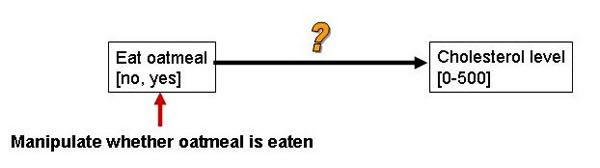
\includegraphics{../images/cholesterolcausaldiagram1.jpg}
\end{center}
 \caption{Hypothetical experimental design---hypothesis only.}
\label{fig: cholestrol1}
\end{marginfigure}


This causal graph shows a simple experiment with two variables:
 \begin{longtable}[!t]{ | P{4cm} | P{3cm} | P{1.5cm} | }
\hline
\tahead{Type of Variable}&\tahead{Variable}&\tahead{Values} \\ \hline
Independent variable --- manipulated&Eat oatmeal&no,yes \\ \hline
Dependent variable&Cholesterol level&0-500 mg/dl \\ \hline
\caption{Variables in sample experimental design}
\label{table: variables}
\end{longtable}


Thus, researchers begin with a random (or representative) sample from the actual population, and divide that group into sub-samples. In one of the simplest experimental designs, the independent variable has one value that is thought to affect the dependent variable (often called the \emph{treatment} condition) and a neutral value that is thought to have no effect (often called the \emph{control condition}). The experimental manipulation involves delivering the value that is thought to affect the DV to one sample, known as the \emph{experimental} or \emph{treatment group}, and the neutral value to the other sample, known as the \emph{control group}.

\begin{itemize}
\item The \emph{experimental group} receives the experimental treatment. It functions as a sample of the hypothetical population in which everyone received the experimental treatment

\item The \emph{control group} acts as if it were a sample of the hypothetical population in which no one received the experimental treatment

\end{itemize}

To determine whether eating oatmeal affects cholesterol levels, we will focus on the difference between the means for the variable cholesterol level for both the experimental and control group and determine whether the difference is statistically significant. If it is, we conclude that eating oatmeal ¾ cup of oatmeal per day does cause lower cholesterol. If, on the other hand, there is no difference or the difference is too small to be statistically significant, we conclude that this study failed to provide evidence of a causal connection.

\newthought{Generally only one or a few variables} are used to differentiate the experimental from the control group. But there are many other variables on which individuals may very. For example, if you were a subject in the cholesterol study, other factors in your life may have changed during the period you were eating cholesterol every day. 

\begin{marginfigure}
 \begin{center}

  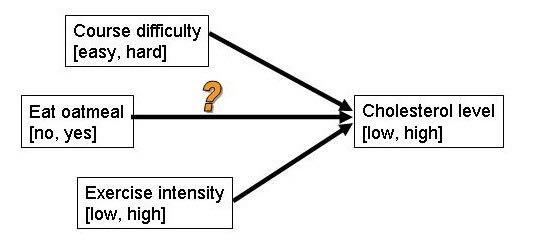
\includegraphics{../images/cholesterolcausaldiagram.jpg}
\end{center}
 \caption{Hypothetical experimental design with auxiliary hypotheses.}
\label{fig: cholestrol-withauxiliary}
\end{marginfigure}
Maybe you took up ultimate frisbee during this time, and the vigorous exercise was responsible. Or you were taking a very difficult course, and studying hard made the difference. Thus, from your results alone we cannot distinguish between \fullref{fig: cholestrol-withauxiliary}.

These additional variables are known as \emph{extraneous variables}. In many instances we can be pretty confident that these additional variables will not affect the outcome of the study. For example, deciding to dye your hair or acquiring a cat is not likely to affect your cholesterol levels. But in some cases the variable just might be a causal factor for the dependent variable under investigation. If it does influence the outcome of the study, it is known as a \emph{confounding variable}.

\begin{thesis}[Confounding Variables]\label{thesis:confoundingvariables}Confounding variable: an extraneous variable that co-varies in the experiment with the IV or DV; if it happens to be causally related to the IV or DV, the internal validity of the experiment (the ability of the experiment to test what it tries to test) is compromised. \newline
<<<<<<< HEAD
A confounding variable is frequently simply called a ‘confound.’\end{thesis}

\newthought{Confounding variables can arise} at many different points in the experiment. There may be differences between the subjects comprising the experimental and control group. If some other variable is inequality distributed across the two experimental groups, it could be the cause of the difference observed in the DV. 

If the difference is between subjects, the variables are known as \emph{subject variables.}

If the difference is between the procedures followed for the two groups, the variables are known as \emph{procedural variables.}

\newthought{It often takes real detective work} to identify confounds in an experiment. Take the case of Wilhelm von Osten, who in 1900 purchased an arab stallion from Russia named Hans. Convinced that animals were more intelligent than usually thought, von Osten set out to teach Hans simple arithmetic. Von Osten presented arithmetic problems to Hans on a chalkboard, and Hans responded by taping his foot the appropriate number of times. Hans seemed to be able to solve even fairly complicated problems including the taking of square roots. Although many were skeptical, numerous mathematicians were brought in to test the horse, and some even concluded that his mathematical abilities equaled those of 14 year old school children.

\begin{figure*}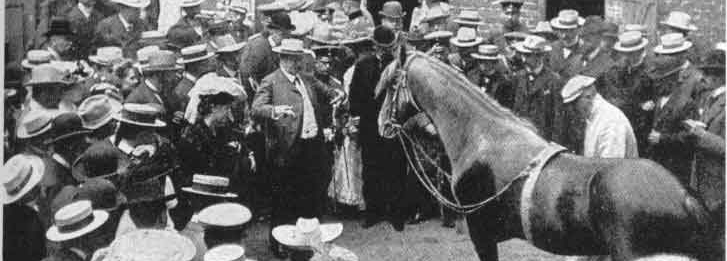
\includegraphics{../images/CleverHans.jpg}\caption{Clever Hans---By Karl Krall (Karl Krall, Denkende Tiere, Leipzig 1912, Tafel 2) Public domain, via Wikimedia Commons}\label{fig:cleverhans}\end{figure*}

\begin{marginfigure}
\begin{center}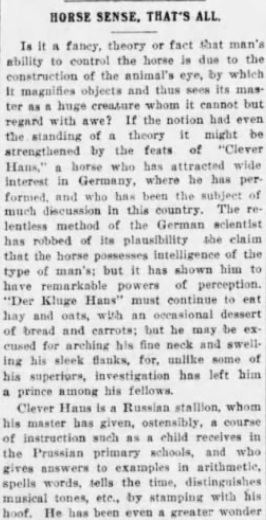
\includegraphics{../images/cleverhansarticle.png}\end{center}
\caption{Article reporting on Clever Hans, from Democrat and Chronicle, Rochester NY, published Aug 5, 1906.}
\label{fig:cleverhansarticle}
\end{marginfigure}To answer skeptics, von Osten brought together a group of two zoologists, a psychologist, a horse trainer, and a circus manager to study Hans over several weeks. Hans performed brilliantly until the psychologist, Oskar Pfungst, varied the experimental setup to conceal the problem from all the humans in the room. The person who wrote the problem on the board was required to leave before the horse entered. 

Under these conditions, Hans dropped from scoring 9 out of 10 to 1 out of 10. This suggested that Hans was picking up a subtle, inadvertent cue from one of the humans and using that to decide when to stop tapping his foot.

Once it became clear that there was some other cue Hans was using, interest in him diminished. But if you were interested in discovering just what cue Hans was responding to, more experiments would be needed. 

\newthought{There are several ways possible} confounding variables can be dealt with in a study. Consider the following example:

\begin{apatextbox}{Nightlights and myopia}
Research at the University of Pennsylvania and the Children’s Hospital of Philadelphia indicates that children who sleep in a dimly lighted room until age two may be up to five times more likely to develop myopia (nearsightedness) when they grow up.\newline
The researchers asked the parents of children who had been patients at the researcher’s eye clinic to recall the lighting conditions in the children’s bedroom from birth to age two.\newline
Of a total of 172 children who slept in darkness, 10 percent were nearsighted.  Of a total of 232 children who slept with a night light, 34 percent where nearsighted.  Of a total of 75 who slept with a lamp on, 55 percent were nearsighted.\newline
The lead ophthalmologist, D. Graham E. Quinn, said that, “just as the body needs to rest, this suggests that the eyes need a period of darkness” 
\end{apatextbox}

Dr. Quinn is claiming that there is a relationship between the amount of darkness experienced by children and the rate of myopia in those children when they are older. In short, that lack of exposure to darkness may cause nearsightedness.

We have two variables to consider: the amount of light when sleeping as an infant, and myopia at 5 years old. The first thing any scientific study has to do define how those variables will be measured. Recall from \fullref{theparadigminexperimentalpsychology:hermannebbinghaus} that Ebbinghaus’ real contribution to scientific psychology was the care he took in defining how memory and recall could be measured quantitatively. 

In this case, the researchers define two variables, as diagramed in \fullref{fig:hypothesis2}
\begin{figure*}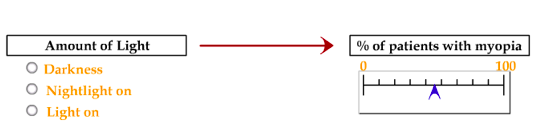
\includegraphics{../images/hypothesis2.png}\caption{First representation of the experiment, with both variables defined}\label{fig:hypothesis2}\end{figure*}
\newthought{Confounding variables} In the University of Pennsylvania study, the first variable is measured by memory---the researchers “asked the parents to recall the lighting conditions.” Individual memories are not the most reliable measurement. 

This would only be a problem \emph{if} there was reason to think that the group of parents would systematically skew their memories in some way. To put it another way: if the rate of mis-remembering was constant across all the parents surveyed, then the effect of mis-remembering would be equal in the IV groups. Any difference in the DV would be due to the \emph{differences} between the IV groups, and hence, cannot be the result of the equalized mis-remembering. Therefore, there is no reason to think that inaccurate remembering would change the results of the study significantly.

So what we have to ask, to assess whether or not this experiment is valid, is if there is a way in which the memories of the parents would be systematically skewed according to their grouping. 

We need to figure out if, perhaps, we have a situation like in diagram \fullref{fig:hypothesis3}:

\begin{figure*}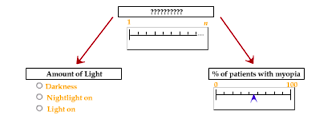
\includegraphics{../images/hypothesis3.png}\caption{Second representation of the experiment, possible confound included}\label{fig:hypothesis3}\end{figure*}

That there is some unknown third variable that increases the chances of \emph{both} myopia in children and the use of nightlights.

What about ‘vision problems in the parents’? It would stand to reason that parents with vision problems are more likely to have children with vision problems. And it is certainly possible that parents with vision problems would be more likely to use nightlights, so they could enter the child’s room without tripping over anything left laying about.

‘Vision problems in the parents’ is a ‘confounding’ variable---and an corrected study would ‘control’ the confound by ensuring that families participating in the study did not have vision problems of their own, or that for every family with vision problems in the ‘light on’ group, there is a family with similar problems in each of the other two groups.

\newthought{This study lacks internal validity}.. Internal validity looks inside the experiment to its design. The central question of internal validity is: Was the experiment designed so as to determine what was really happening?
\begin{thesis}[Internal validity]
The extent to which a study’s design ensures that its result will be in accordance with reality. That is, if the suspected cause really is a cause, the predicted effect on the DV is confirmed; if not, the predicted effect on the DV is not confirmed. To ensure this, other possible causes must be well-controlled.
\end{thesis}

Second, notice that the families in this study were recruited from patients of the eye clinic doing the study. Eye clinics, even in famous hospitals, serve the resident population. The University of Pennsylvania Hospital likely treats families who live in and around Philadelphia. That means that this population is systematically skewed towards an urban population.

I have no idea if that means that mis-remembering could be higher than normal. But I do know, having lived in Philadelphia for graduate school---near the University of Pennsylvania---that there is a great deal of light pollution. Thus, even if the study were internally valid, it would not be applicable to families living in a rural environment, where complete darkness is possible at night, unlike in an urban environment.\begin{thesis}[External validity]
the extent to which a study’s results can be generalized. (Relevant questions include: were the participants sampled from a broad population or narrow one? Were they selected in a way that assured they were representative of the population? How well can we describe the population they were sampled from?)\newline
It is also called ‘Generalizability’
\end{thesis}

This lack of generalizability is called ‘external validity’. It is defined in the margin to the right. External validity, looks outside the experiment itself to what conclusions can be drawn from the resulting data.

\subsubsection{Assessing Validity}
\label{assessingvalidity}

Let’s consider another example:

\begin{apatextbox}{Vasectomy Study}
New studies reported in the Journal of the American Medical Association indicate that vasectomy is safe.  A group headed by Frank Massey of UCLA paired 10,500 vasectomized men with a like number of men who had not had the operation.  The average follow-up time was 7.9 years, and 2,300 pairs were followed for more than a decade.  The researchers reported that, aside from inflammation of the testes, the incidence of diseases for vasectomized men was similar to that in their paired controls.\newline
A second study done under federal sponsorship at the Battelle Human Affairs Research Centers in Seattle compared heard disease in 1,400 vasectomized me and 3,600 men who had not had the operation.  Over an average follow-up time of fifteen years, the incidence of heart diseases was the same among men in both groups. \end{apatextbox}

The study has well defined variables, and standard measurements. That’s good. But why are they paring men who had a vasectomy with men who did not? We’ve diagrammed the study’s logic in figure \fullref{fig:hypothesis4}.
\begin{figure*}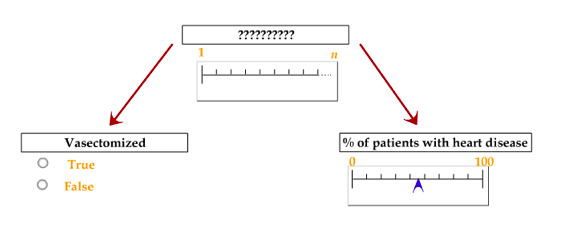
\includegraphics{../images/hypothesis4.png}\caption{Diagram of Vasectomy study}\label{fig:hypothesis4}\end{figure*}

There might be some third cause that affects whether or not men get vasectomies that \emph{also} effects their rate of heart disease. This is not too hard to imagine: what kind of men get vasectomies? Well, heterosexual men in long-term, probably married, relationships. And it is likely that these men have healthier lifestyles and diets than their non-married counterparts. 

It is very difficult, if not impossible to control for all the factors that make up ‘lifestyle.’ But with a large enough sample, that matched individuals with and without a vasectomy according to ‘lifestyle’, all those differences would drop out of the statistics as irrelevant. This is diagramed in \fullref{fig:hypothesis5}.

\begin{figure*}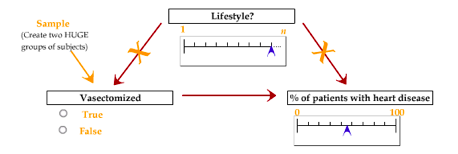
\includegraphics{../images/hypothesis5.png}\caption{Diagram of vasectomy study with controls in place.}\label{fig:hypothesis5}\end{figure*}

\newthought{Any factor \emph{other} than the independent variable} that alters the dependent variable can affect the internal validity of an experiment. 

Randomizing the assignment of subjects to the experimental and control conditions overcomes many of the potential dangers to internal validity. If randomization is effective, all other pre-existing subject variables that may affect the dependent variable appear in the two groups at equal rates, leaving only the independent variable as the source of difference between the groups. With small samples, however, even randomization can result in other factors being unequally distributed between the experimental and control groups. 

Even if the randomization does equalize all pre-existing factors that might affect the dependent variable, other conditions might arise during the experiment that have an effect. For example, perhaps the experimental and control groups are sent to different rooms, and the rooms are of different temperatures. If you were measuring impatience or irritation, there could be large effects in your dependent variable based on the temperature of the room.

Another set of internal validity concerns arise from two sources of bias. Both experimenter bias and subject reactivity can compromise an experiment. Often, though not always, participants can be kept ``blind'' as to what condition they are in or what the experimenter expects. If the experimenter also is ``blind'' as to which participants are in which conditions, it is a ``double-blind'' experiment. The most familiar example is drug studies, in which neither the participants nor the experimenter know who is getting the investigational drug and who is getting a placebo.

\newthought{For a study to have external validity}, its results must be generalizable to the intended target population. But often researchers only study a small part of the target population, or even another population altogether. For example, in both biological and biomedical research, studies are conducted on other species, but the conclusions are applied to humans. Before testing a new drug on humans, for example, it is first tested on mice or rats or other creatures. In psychological research, college undergraduates are often used as subjects, but inferences are made about humans in general. External validity is the extent to which results can be generalized to the population as a whole.

The very fact of an experiment can, with humans, produce results that would not happen otherwise. Imagine that you are walking across campus and a total stranger who looks like a fellow student walks up to you and asks you to turn around and walk backwards for 20 feet. Will you do it? Now imagine that the stranger prefaces her request with “I am conducting an experiment for my psychology class” and then proceeds with the same request. Are you more likely to comply? If so, then compliance in an experiment may be a product of the experiment and not indicative of behavior outside of that situation.

\subsubsection{What all experimental design has in common}
\label{whatallexperimentaldesignhasincommon}

\begin{itemize}
\item Intervene in some way to change the value of the IV, measurement of the DV.

\item Efforts are made to control extraneous variables.

\end{itemize}

\subsubsection{Common threats to internal validity}
\label{commonthreatstointernalvalidity}

\begin{itemize}
\item No Control Group

\item Nonequivalent Control Groups

\item No adequate measurement of DV or using an unverified measures

\item Pre-Test Post-Test Pitfalls:

\begin{itemize}
\item Maturation---if there is a great deal of time between the pre- and post-test, it is possible than any possible result comes from the maturation of the participants, not the intervention.

\item Testing fatigue---as with standardized testing in high school, participants may become annoyed or bored with the testing, and hence produce poor results.

\item Instrument Decay---if the instrument ‘drifts’ or changes over time, internal validity would suffer. This is particularly a problem when the measurement is based on coding or classification.

\item Regression to the mean---with repeated measures, results tend towards the mean. An initially promising result may just be an outlier, which would prove to be insignificant with repeated measures.

\end{itemize}

\item P-value hacking---Statistical significance is usually measured with p$<$0.05. 0.05\% is one in twenty, which is to say that if a ‘statistically significant’ result has a 1 in 20 chance of having been random noise, rather than an actual effect. Given powerful statistical software we have now, an unscrupulous research could just run his or her data 20 times, or until a statistically significant result appears.

\end{itemize}

\subsubsection{Common experimental designs}
\label{commonexperimentaldesigns}

\newthought{Two Groups, Post-Test only}

\begin{itemize}
\item Subjects assigned to control or experimental group randomly, Dependent variable is tested after the independent variable is introduced.

\end{itemize}

\newthought{Two Groups, Pre-Test and Post-Test}

\begin{itemize}
\item Same as above, except that a pre-test is given to ensure the equivalence of the two groups.

\end{itemize}

\newthought{Simple Random Assignment}

\begin{itemize}
\item Just what it sounds like: randomly assign each subject to one of the groups (a coin flip is sufficient for two groups).

\end{itemize}

\newthought{Matched Pairs Assignment}

\begin{itemize}
\item First match subjects into pairs based on some characteristic related to the IV.  Then randomly assign the members of each pair to one of the two experimental groups.

\item The same individuals participate in both experimental conditions, after which the dependent variable is measured.

\item Advantages: Fewer individuals are required.

\item If training (or acclimatizing) is required, this design can save valuable resources.

\item As the individuals in the experimental conditions are identical, more confounds are controlled.

\end{itemize}

One way to explain why something happens is to demonstrate a cause for it. But causes typically do not operate in isolation. Encountering a virus may explain why you developed the flu, but the condition of having the flu only arises when a number of other things happen. In particular, a virus must invade a particular cell (flu viruses invade cells lining a person’s respiratory or digestive track). 

Except for the fact that some viruses break out of their generous hosts by breaking the host cell open and killing it, this all sounds harmless enough. But the consequences are what debilitate you:

\begin{itemize}
\item When the cells lining the respiratory track are killed, fluid can flow into your nasal passages; this is what you experience as a runny nose.

\item This nasal fluid contains more viruses and as they drip down your throat they attack the cells lining it. You experience this as a sore throat.

\item The virus particles that get into your bloodstream attack muscle cells, which you experience as muscle ache.

\item Finally, you body is designed to resist this assault. One thing it does is produce pyrogens, chemicals that cause your body temperature to increase. The higher temperature reduces the capacity of cells to carry out their operations, including hosting the creation of new viruses.

\end{itemize}

Although it was the virus that caused the flu, a lot of other operations were going on. The virus had to rely on a complex bit of machinery to carry out its task of reproducing itself, and in the process laying you low with the flu.

\begin{marginfigure}
 \begin{center}

     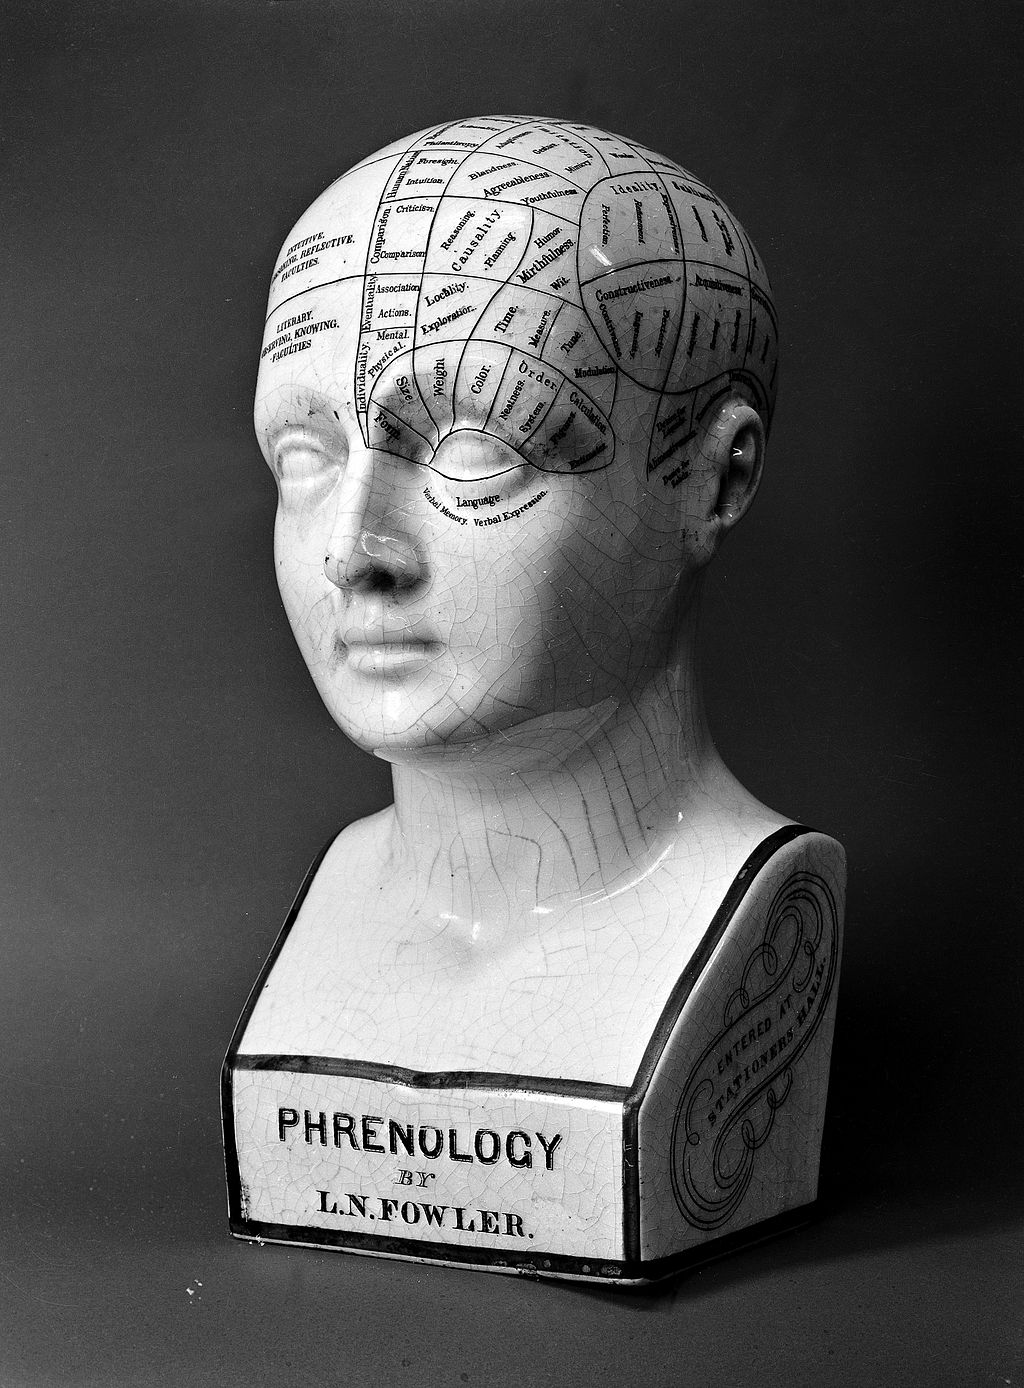
\includegraphics{../images/phrenology.jpg}
\caption{Mechanistic explanation is not new to science. In the 19th century, Franz Joseph Gall suggested phrenology, which sought to identify particular mechanisms of intelligence with particular bumps on the skull. The mechanism posited held that personality traits were localized in the brain, and the brain would be enlarged in specific areas for those traits. The enlargements could then be detected by the structure of the skull. We still accept the idea of localization, but unlike muscles, excess activity does not make the brain enlarge. Image from Wikimedia Commons}
\end{center}
\label{fig:phrenology}
\end{marginfigure}

The explanatory scenario just outlined, in which we invoke a mechanism to explain a causal effect, is extremely common in science.

\begin{itemize}
\item To explain the reproduction of cells, scientists describe the \emph{mechanism} of cell reproduction.

\item To explain how blood carries nutrients to tissues in the body, they describe the \emph{mechanism} of circulation of the blood.

\item To explain how people can remember events in their lives and new factual information, they describe the mechanisms of memory encoding, storage, and retrieval.

\end{itemize}

\begin{thesis}[Mechanism definition]
Mechanism: entities and activities organized so that a phenomenon occurs or entities and activities organized in such a way as to realize a function.
\end{thesis} 

Explaining the occurrence of a phenomenon by identifying the mechanism that produces it is perhaps the most common explanatory strategy in science. Accordingly, we need to consider in detail

\begin{itemize}
\item what a mechanism is

\item how mechanisms are described

\item how mechanisms are discovered

\item how mechanisms are modeled

\item how accounts of mechanism are tested.

\end{itemize}

When scientists use the word ‘mechanism’, they are talking about an explanation that decomposes into other entities, and explains behavior in terms of the interactions of those entities’ behaviors. They are discovered with three basic techniques\footnote{This section is based on the work of my collaborators, William Bechtel (~\citep{Bechtel:2010we} and ~\citep{Bechtel:OYBoWb_-}) and Carl Craver (~\citep{Craver:2006ti}).}:

\newthought{Recording activity.} The simplest intervention on a mechanism is to record the activity of the underlying entities. Consider by analog a steam-engine. If one wanted to figure out how it worked, one would have to turn it on, and record the activity of its parts: the boiler does such and such, the pistons move{\ldots} etc.

\newthought{Stimulating components.} If components of a mechanism are distinct, they should be able to be stimulated directly. The Penfield Homunculus for example, was created by direct stimulation of a patient’s brain, and recording which parts of his body reacted.\begin{marginfigure}
 \begin{center}

     
\includegraphics{../Images/Motor_homunculus.png}

\end{center}
 \caption{Penfield Homunculus, from wikiimages}
\label{fig: MattachinePamphlet}
\end{marginfigure}


\newthought{Inhibiting components.} Some times called ‘lesioning’, this strategy is simply to block the activity of a component of a mechanism, and see record the activity of the whole, or the activity of the other components in the absence of the component of interest. We know, for example, that the hippocampus plays a significant role in personal memory because we have a observed a patient (HM), who has his hippocampus removed surgically. ~\citep{Scoville:1957wx}

A posited mechanism must allow for at least these three methods of investigation to be considered scientific. Mechanistic explanations that do not allow for recording of the activity, stimulating, or inhibiting of components can’t be considered a scientific explanation. 

\subsubsection{What all mechanistic explanation has in common}
\label{whatallmechanisticexplanationhasincommon}

\begin{itemize}
\item Posits entities and activities that are arranged in such a way that their interaction produces the phenomenon in question.

\item Entities and activities must be, in principle:

\begin{itemize}
\item Measurable

\item Stimulatable

\item Inhibitable

\end{itemize}

\end{itemize}

\subsection{Ethics of human research}
\label{ethicsofhumanresearch}

Ethical codes of research have generally followed the discovery or publication of horrifically unethical experiments. The most famous of these is probably the Nuremberg Code, adopted by the international medical community after the discovery of the Nazi `experiments' performed on Jews, Homosexuals and Gypsies during the Holocaust. The Nuremberg code is available online, and should be reviewed by anyone proposing an experiment or sitting on the Research Committee. 

\subsubsection{The Nuremberg Code}
\label{thenurembergcode}

The Nuremberg code (~\citep{TheNationalInstitutesofHeath:2009vr}) lays out ten simple principles for design experiments on humans. They are:

\begin{apatextbox}{The Nuremberg Code} 

\rowgroup{1.    The voluntary consent of the human subject is absolutely essential. This means that the person involved should have legal capacity to give consent; should be so situated as to be able to exercise free power of choice, without the intervention of any element of force, fraud, deceit, duress, overreaching, or other ulterior form of constraint or coercion; and should have sufficient knowledge and comprehension of the elements of the subject matter involved as to enable him to make an understanding and enlightened decision. This latter element requires that before the acceptance of an affirmative decision by the experimental subject there should be made known to him the nature, duration, and purpose of the experiment; the method and means by which it is to be conducted; all inconveniences and hazards reasonably to be expected; and the effects upon his health or person which may possibly come from his participation in the experiment.\newline

The duty and responsibility for ascertaining the quality of the consent rests upon each individual who initiates, directs, or engages in the experiment. It is a personal duty and responsibility which may not be delegated to another with impunity.}\\

\rowgroup{2.    The experiment should be such as to yield fruitful results for the good of society, unprocurable by other methods of means of study, and not random and unnecessary in nature.}\\

\rowgroup{3.    The experiment should be so designed and based on the results of animal experimentation and a knowledge of the natural history of the disease or other problem under study that the anticipated results will justify the performance of the experiment. }\\

\rowgroup{4.    The experiment should be so conducted as to avoid all unnecessary physical and mental suffering and injury.}\\

\rowgroup{5.    No experiment should be conducted where there is an a priori reason to believe that death or disabling injury will occur; except, perhaps, in those experiments where the experimental physicians also serve as subjects.}\\

\rowgroup{6.    The degree of risk to be taken should never exceed that determined by the humanitarian importance of the problem to be solved by the experiment. }\\

\rowgroup{7.    Proper preparations should be made and adequate facilities provided to protect the experimental subject against even remote possibilities of injury, disability or death.}\\

\rowgroup{8.    The experiment should be conducted only by scientifically qualified persons. The highest degree of skill and care should be required though all stages of the experiment of those who conduct or engage in the experiment. }\\

\rowgroup{9.    During the course of the experiment the human subject should be at liberty to bring the experiment to an end if he has reached the physical or mental state where continuation of the experiment seems to him to be impossible.}\\

\rowgroup{10.   During the course of the experiment the scientist in charge must be prepared to terminate the experiment at any stage, if he has probable cause to believe, in the exercise of the good faith, superior skill and careful judgment required of him that a continuation of the experiment is likely to result in injury, disability or death to the experimental subject. }\\

\end{apatextbox}
 

\subsubsection{The Declaration of Helsinki}
\label{thedeclarationofhelsinki}

In 1964, the medical community through the World Medical Association adopted the `Declaration of Helsinki', which replaced the Nuremberg code as the standard for ethical experimentation on humans by the medical community. (~\citep{Association:1975wh}) The World Medical Association still maintains the Declaration, adopting the most recent revisions in 2004. Current versions are available online.

Psychiatrists, as practicing medical doctors, are bound by the Declaration of Helsinki. While it is far more complete than the Nuremberg code, the same basic ideas appear:

\begin{apatextbox}{The Declaration of Helsinki}
\label{sample:helsinki} 


I. Basic Principles \\

\rowgroup{1. Biomedical research involving human subjects must conform to generally accepted scientific principles and should be based on adequately performed laboratory and animal experimentation and on a thorough knowledge of the scientific literature. }\\

\rowgroup{2. The design and performance of each experimental procedure involving human subjects should be clearly formulated in an experimental protocol which should be transmitted to a specially appointed independent committee for consideration, comment and guidance. }\\

\rowgroup{3. Biomedical research involving human subjects should be conducted only by scientifically qualified persons and under the supervision of a clinically competent medical person. The responsibility for the human subject must always rest with a medically qualified person and never rest on the subject of the research, even though the subject has given his or her consent. }\\

\rowgroup{4. Biomedical research involving human subjects cannot legitimately be carried out unless the importance of the objective is in proportion to the inherent risk to the subject. }\\

\rowgroup{5. Every biomedical research project involving human subjects should be preceded by careful assessment of predictable risks in comparison with foreseeable benefits to the subject or to others. Concern for the interests of the subject must always prevail over the interests of science and society. }\\

\rowgroup{6. The right of the research subject to safeguard his or her integrity must always be respected. Every precaution should be taken to respect the privacy of the subject and to minimize the impact of the study on the subject's physical and mental integrity and on the personality of the subject. }\\

\rowgroup{7. Physicians should abstain from engaging in research projects involving human subjects unless they are satisfied that the hazards involved are believed to be predictable. Physicians should cease any investigation if the hazards are found to outweigh the potential benefits. }\\

\rowgroup{8. In publication of the results of his or her research, the physician is obliged to preserve the accuracy of the results. Reports of experimentation not in accordance with the principles laid down in this Declaration should not be accepted for publication. }\\

\rowgroup{9. In any research on human beings, each potential subject must be adequately informed of the aims, methods, anticipated benefits and potential hazards of the study and the discomfort it may entail. He or she should be informed that he or she is at liberty to abstain from participation in the study and that he or she is free to withdraw visor her consent to participation at any time. The physician should then obtain the subject's freely given informed consent, preferably inheriting.} \\

\rowgroup{10. When obtaining informed consent for the research project the physician should be particularly cautious if the subject is in dependent relationship to him or her or may consent under duress. In that case the informed consent should be obtained by a physician who isn't engaged in the investigation and who is completely independent of this official relationship. }\\

\rowgroup{11. In case of legal incompetence, informed consent should be obtained from the legal guardian in accordance with national legislation. Where physical or mental incapacity makes it impossible to obtain informed consent, or when the subject is a minor, permission from the responsible relative replaces that of the subject in accordance with national legislation. Whenever the minor child is in fact able to give a consent, the minor's consent must be obtained in addition to the consent of the minor's legal guardian. }\\

\rowgroup{12. The research protocol should always contain a statement of the ethical considerations involved and should indicate that the principles enunciated in the present declaration are complied with. }\\

II. Medical Research Combined with Professional Care (Clinical Research) \\

\rowgroup{1. In the treatment of the sick person, the physician must be free to use a new diagnostic and therapeutic measure, if in his or her judgement it offers hope of saving life, re-establishing health or alleviating suffering. }\\

\rowgroup{2. The potential benefits, hazards and discomfort of a new method should be weighed against the advantages of the best current diagnostic and therapeutic methods. }\\

\rowgroup{3. In any medical study, every patient- including those of a control group, if any- should be assured of the best proven diagnostic and therapeutic method. }\\

\rowgroup{4. The refusal of the patient to participate in a study must never interfere with the physician-patient relationship. }\\

\rowgroup{5. If the physician considers it essential not to obtain informed consent, the specific reasons for this proposal should be stated in the experimental protocol for transmission to the independent committee (1, 2). }\\

\rowgroup{6. The physician can combine medical research with professional care, the objective being the acquisition of new medical knowledge, only to the extent that medical research is justified by its potential diagnostic or therapeutic  value for the patient. }\\

III. Non-Therapeutic Biomedical Research Involving Human Subjects (Non-Clinical Biomedical Research) \\

\rowgroup{1. In the purely scientific application of medical research carried out on a human being, it is the duty of the physician to remain the protector of the life and health of that person on whom biomedical research is being carried out. }\\

\rowgroup{2. The subjects should be volunteers- either healthy persons or patients for whom the experimental design is not related to the patient's illness. }\\

\rowgroup{3. The investigator or the investigating team should discontinue the research if in his/her or their judgment it may, if continued, be harmful to the individual. }\\

\rowgroup{4.    In research on man, the interest of science and society should never take precedence over considerations related to the well-being of the subject. }\\

 \end{apatextbox}

In the context of psychiatry, of course, the distinction made between therapeutic research and non-therapeutic research is crucially important. If a psychiatric patient were to be deemed incapable of making an informed decision, and there is an experiment therapy that the psychiatrist believes may help, there are few ethical checks and balances to constrain the psychiatrist from performing unwarranted experiments.

\subsubsection{The APA Ethical Standards for Psychologists}
\label{theapaethicalstandardsforpsychologists}

The APA Standards were first published in 1953. (~\citep{Association:71thM4UP}) They were revised in 1958 (~\citep{Association:1958tg}), 1963 (~\citep{Association:1963uu}) and 1968. (~\citep{Association:1968uu}) The 1968 standards, which should guide the research committee in determining which research programs should be allowed to move forward, are attached in Appendix \fullref{app: APAEthics}.

Most of the APA standards outline the responsibilities of psychologists who practice counseling and patient care. While those are incredibly important, we're most concerned here with Principle 16: Research Precautions. In 1958, section 16 was titled `Harmful Aftereffect.' It read:

\begin{apatextbox}{APA Ethical Standards: 1959}\label{sample:APAEthics1959}
\newthought{Principle 16. Harmful Aftereffects}. Only when a problem is significant and can be investigated in no other way is the psychologist justified in giving misinformation to research subjects or exposing research subjects to physical or emotional stress.\\

\rowgroup{a. When the possibility of serious aftereffects exists, research is conducted only when the subjects or the responsible agents are fully informed of this possibility and volunteer nevertheless.}\\

\rowgroup{b. The psychologist seriously considers the possibility harmful aftereffects and removes them as soon as permitted by the design of the experiment.}\\

\rowgroup{c. A psychologist using animals in research adheres to the provisions of the Rules Regarding Animals, drawn up by the Committee on Precautions in Animal Experimentation and adopted by the American Psychological Association.}\\
\end{apatextbox}

Four years later, in 1963, (~\citep{Association:1963uu}) the committee responsible for the Ethical guidelines:

a. Changed the title to `Research Precautions,’ moved the ‘preamble’ to point (a) and added a new preamble. It also changed the phrase `is significant' to `is of scientific significance'; ' can be investigated in no other way' became ' it is not practicable to investigate it in any other way`; ' giving misinformation to research subjects' was dropped; and the phrase `whether children or adults' added to the new point (a).

b. Added the qualification of `reasonable' to `possibility'; changed `harmful' to `injurious' and `volunteer' became `agree to participate'. 

c. Changed `removes' to `avoids or removes'; and 

d. Unchanged.

\begin{apatextbox}{APA Ethical standards 1963}
\label{sample: APAEthics1963}
\newthought{Principle 16. Research Precautions.} The psychologist assumes obligations for the welfare of his research subjects, both animal and human.\\

\rowgroup{a. Only when a problem is of scientific significance and it is not practicable to investigate it in any other way is the psychologist justified in exposing research subjects research subjects, whether children or adults, to physical or emotional stress.}\\

\rowgroup{b. When the possibility of injurious aftereffects exists, research is conducted only when the subjects or the responsible agents are fully informed of this possibility and agree to participate nevertheless.}\\

\rowgroup{c. The psychologist seriously considers the possibility harmful aftereffects and avoids or removes them as soon as permitted by the design of the experiment.}\\

\rowgroup{d. A psychologist using animals in research adheres to the provisions of the Rules Regarding Animals, drawn up by the Committee on Precautions in Animal Experimentation and adopted by the American Psychological Association.} \\
\end{apatextbox}

These changed little between 1963 and 1968 (~\citep{Association:1968uu}), except for the addition of the qualifying phrase `as part of the investigation' to (a) and adding provision (e) governing the use of psychoactive drugs:



\begin{apatextbox}{APA Ethical standards 1968}
\label{sample: APAEthics1968}
\newthought{Principle 16. Research Precautions.} The psychologist assumes obligations for the welfare of his research subjects, both animal and human.\\

\rowgroup{a. Only when a problem is of scientific significance and it is not practicable to investigate it in any other way is the psychologist justified in exposing research subjects research subjects, whether children or adults, to physical or emotional stress as part of an investigation.}\\
\rowgroup{b. When the possibility of injurious aftereffects exists, research is conducted only when the subjects or the responsible agents are fully informed of this possibility and agree to participate nevertheless.}\\
\rowgroup{c. The psychologist seriously considers the possibility harmful aftereffects and avoids, or removes them as soon as permitted by the design of the experiment.}\\
\rowgroup{d. A psychologist using animals in research adheres to the provisions of the Rules Regarding Animals, drawn up by the Committee on Precautions in Animal Experimentation and adopted by the American Psychological Association.}\\
\rowgroup{e. Investigations of human subjects using experimental drugs (for example, hallucinogenic, psychotomimetic, psychedelic, or similar substances) should be conducted only in such settings as clinics, hospitals, or research facilities maintaining appropriate safeguards for the subjects.}\\
\end{apatextbox}
\setlength{\leftskip}{0cm} 

For a historical overview, see ~\citep{Fisher:uAWUHvuo} and ~\citep{Fisher:2003tg}.

\pagebreak 

\chapter{Core Texts}
\label{coretexts}

Freud, Sigmund \emph{Introductory lectures on psychoanalysis}, WW Norton \& Company

Supplementary texts that are covered extensively in the game book

Bacon, F., Jardine, L., \& Silverthorne, M. (1620). The new organon. Cambridge texts in the history of philosophy.

Ebbinghaus, H. (1885). Memory. (H. A. Ruger \& C. E. Bussenius, Trans.) (pp. 1–142).

\pagebreak 

\chapter{Index and Bibliographies}
\label{indexandbibliographies}


\backmatter
\printbibliography[heading=subbibliography]
\printindex




\pagebreak 

Thanks to John Heywood of the University of Lancaster for both the history of linguistics, and understanding the gay community in the UK’s experience with psychology during the same time period.

Sections of ‘Basic Scientific Reasoning’ are adapted from work that I did many years ago with William Bechtel, Adele Abrahamson and Carl Craver on the ‘Inquiry project’ as a Post-Doc at Washington University in St. Louis.

\pagebreak 

 \renewcommand*{\thechapter}{}
\renewcommand*{\thesection}{\Alph{section}}
\setcounter{chapter}{0}
\renewcommand*{\thesubsection}{\arabic{subsection}}



\chapter{Appendicies}
\label{appendicies}

\begin{appendices}
\let\svaddcontentsline\addcontentsline
\renewcommand\addcontentsline[3]{%
  \ifthenelse{\equal{#1}{lof}}{}%
  {\ifthenelse{\equal{#1}{lot}}{}{\svaddcontentsline{#1}{#2}{#3}}}}





\section{Pinel, Philippe. “A Treatise on Insanity”, 1806}
\label{pinelphilippe.“atreatiseoninsanity”1806}

\label{app: Pinel}
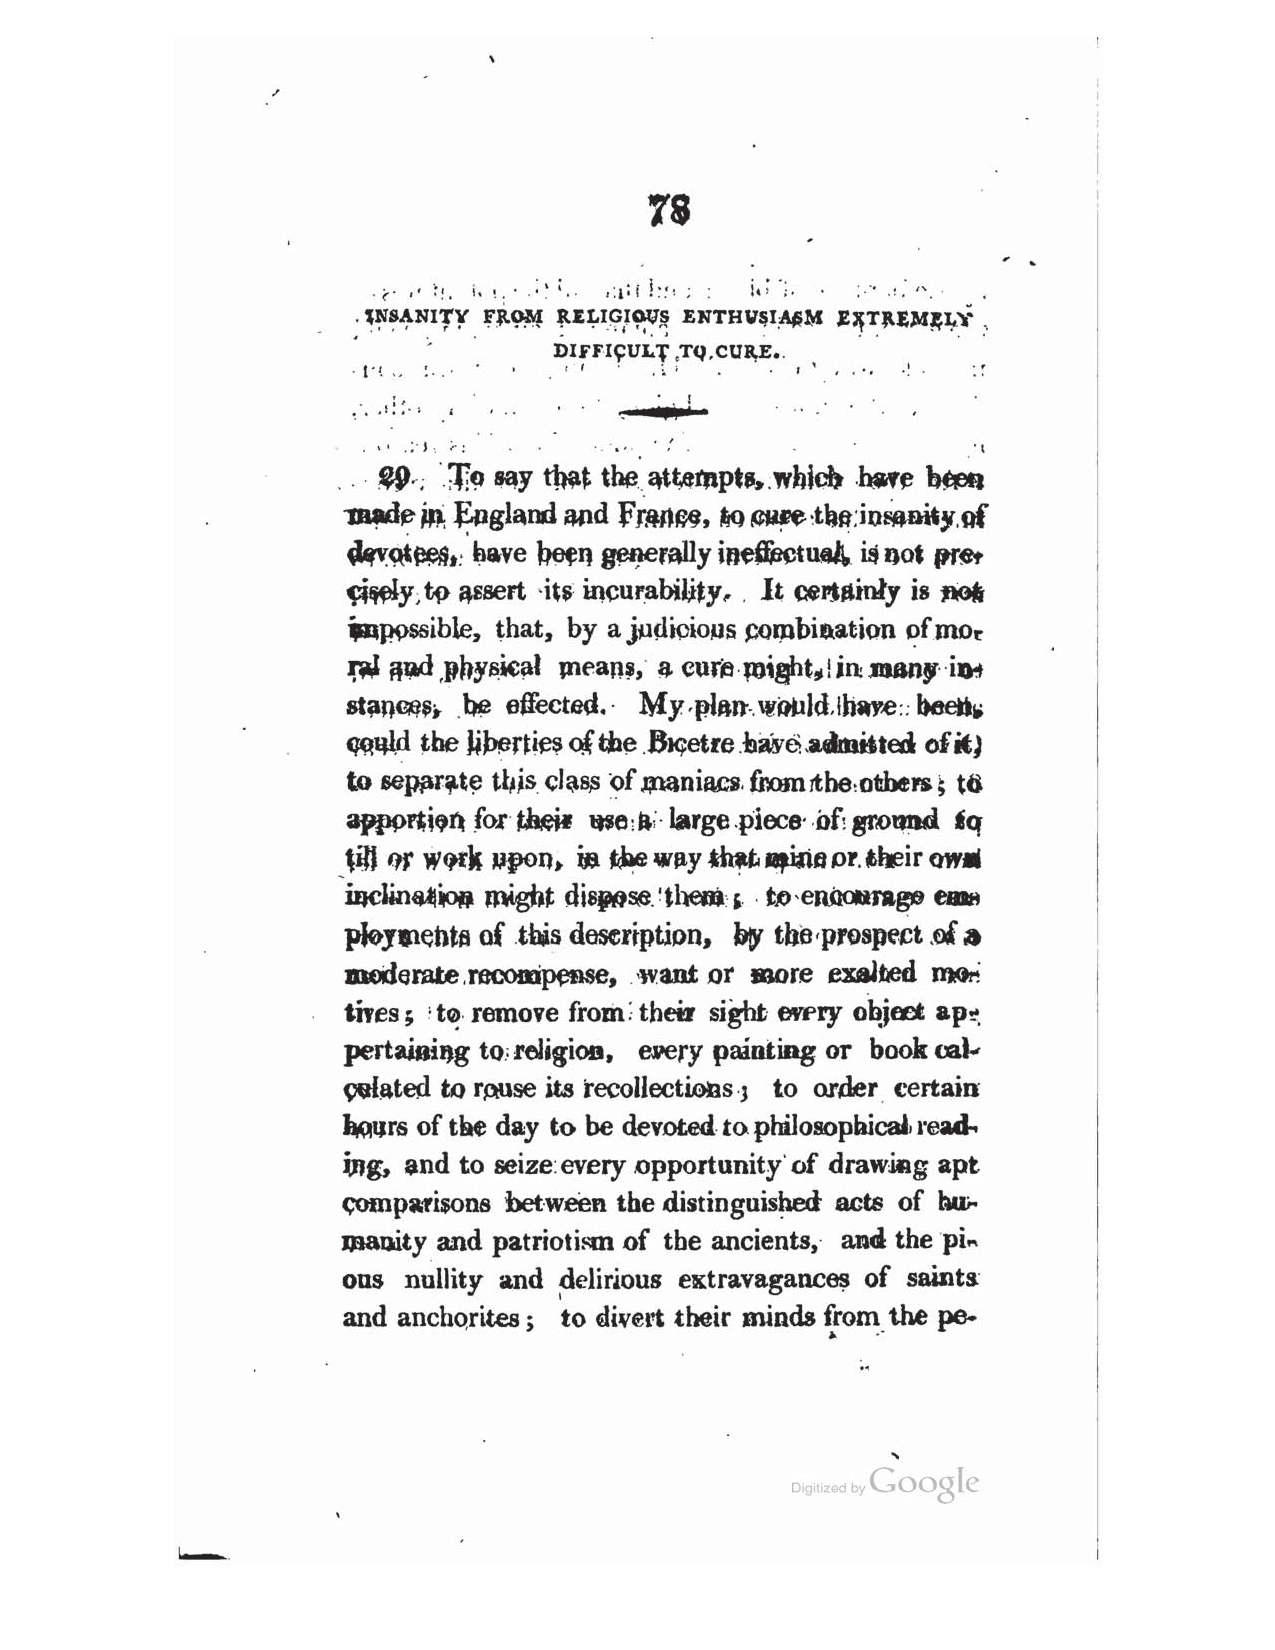
\includepdf[pages={1-}]{../Appendices/1806-Pinel-A_treatise_on_insanity-Excerpt.pdf}

\section{Psychopathia sexualis}
\label{psychopathiasexualis}

\subsection{Excerpt 1}
\label{excerpt1}

\label{app: KraftEbbing1}
\includepdf[pages={1-}]{../Appendices/Excerpt1-1894-Psychopathia_sexualis.pdf}

\subsection{Excerpt 2}
\label{excerpt2}

\label{app: KraftEbbing2}
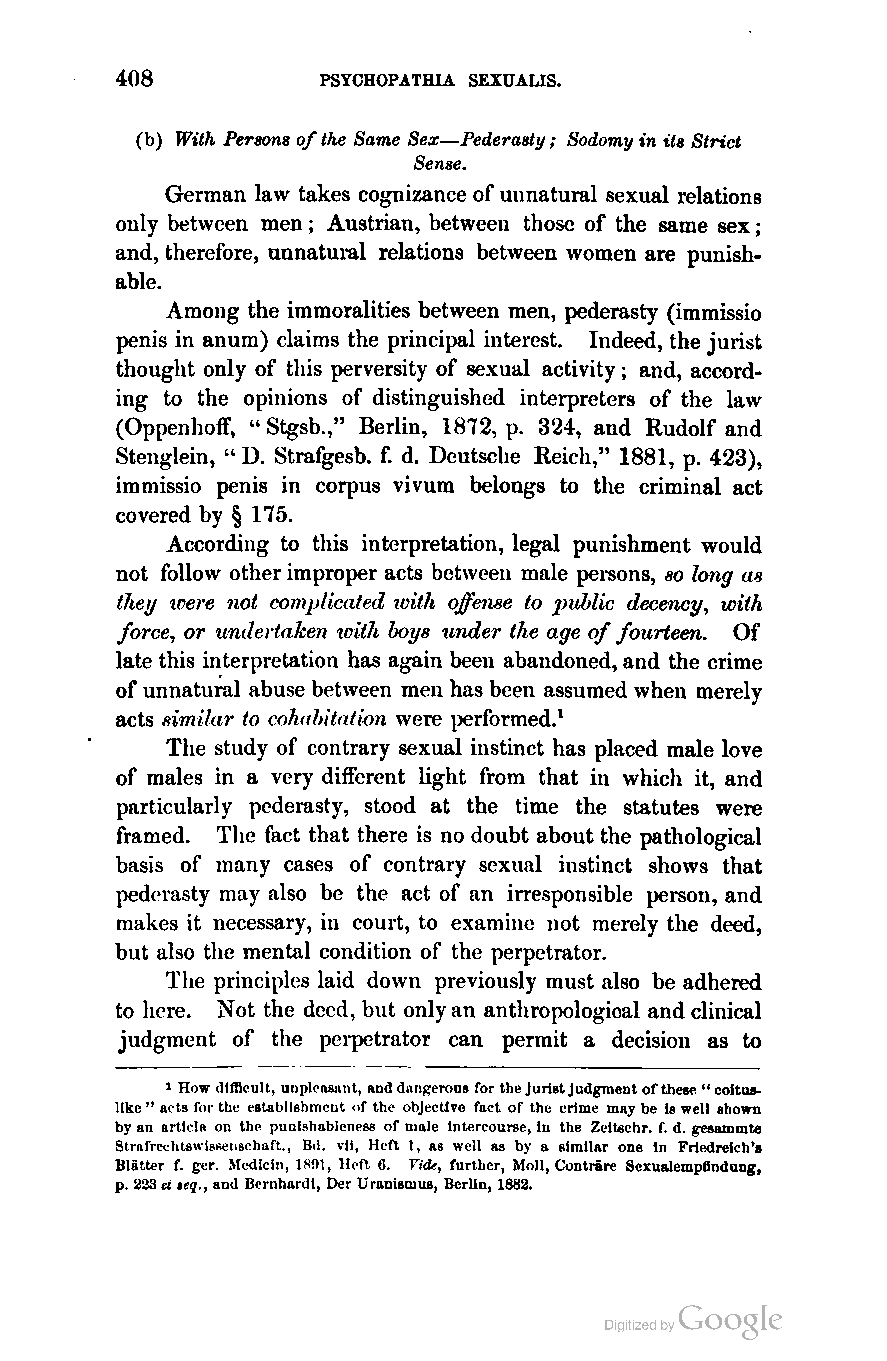
\includepdf[pages={1-}]{../Appendices/Excerpt2-1894-Psychopathia_sexualis.pdf}

\subsection{Excerpt 3}
\label{excerpt3}

\label{app: KraftEbbing3}
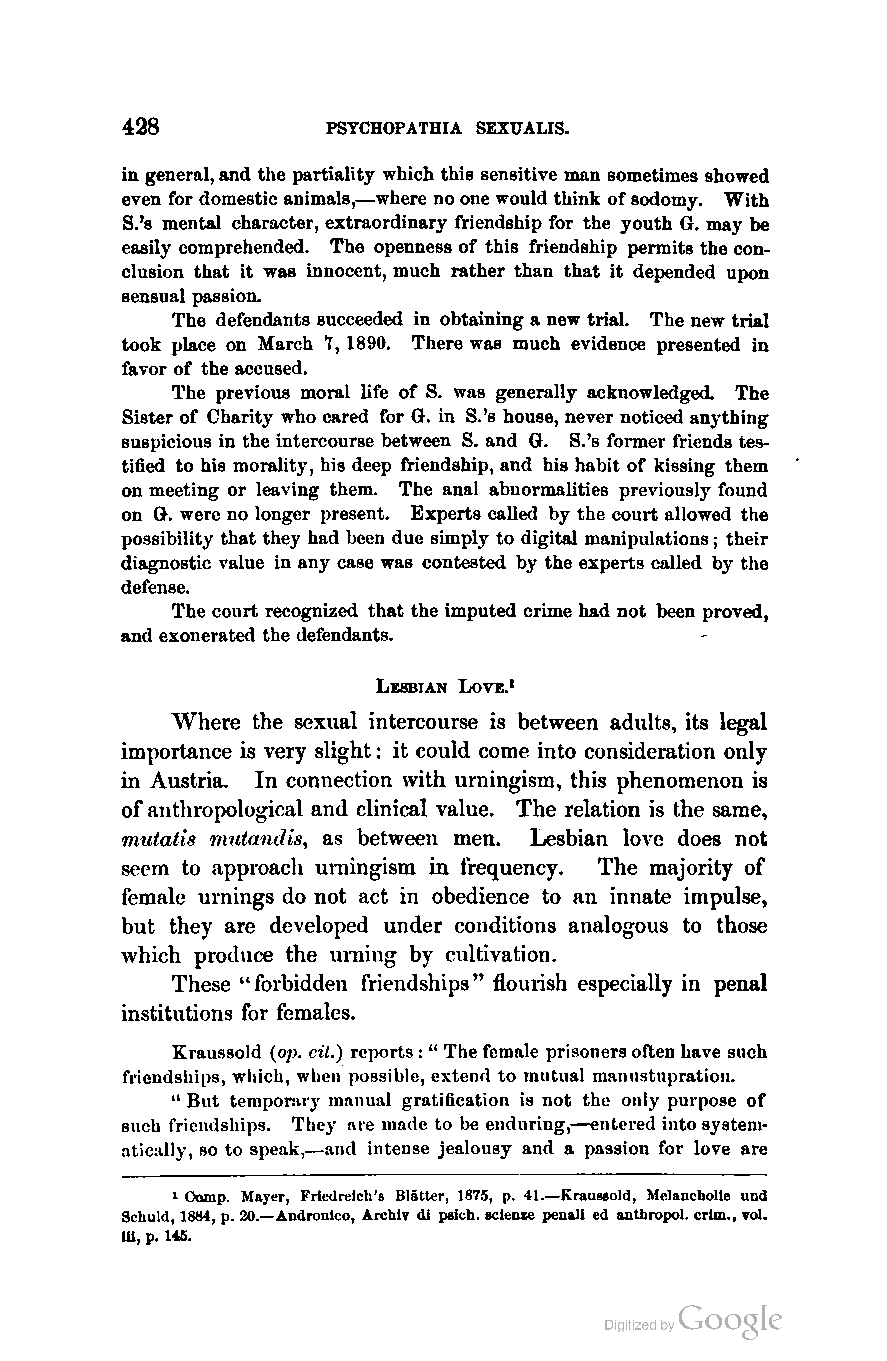
\includepdf[pages={1-}]{../Appendices/Excerpt3-1894-Psychopathia_sexualis.pdf}

\section{Freud, Sigmund “The psychogenesis of a case of homosexuality in a woman” (1920)}
\label{freudsigmund“thepsychogenesisofacaseofhomosexualityinawoman”1920}

\label{app: Freud}
\includepdf[pages={1-}]{../Appendices/1920-Freud-HomosexualityInAWoman.pdf}

\section{Skinner, B. F. “A Critique of Psychoanalytic Concepts and Theories” 1954}
\label{skinnerb.f.“acritiqueofpsychoanalyticconceptsandtheories”1954}

\label{app: Skinner}
\includepdf[pages={1-}]{../Appendices/1954-Skinner.pdf}

\section{Chomsky, N. “Review of \emph{Verbal Behaviour} by B.F. Skinner” 1959}
\label{chomskyn.“reviewofverbalbehaviourbyb.f.skinner”1959}

\label{app: Chomsky}

\includepdf[pages={1-}]{../Appendices/1959-Chomsky-Review.pdf}

\section{APA “Ethical Standards of Psychologists" 1968}
\label{apa“ethicalstandardsofpsychologists1968}

\label{app: APAEthics}
\includepdf[pages={1-}]{../Appendices/APAEthics1968.pdf}

\section{APA \emph{Diagnostic and Statistical Manual} Mental Disorders, 1952}
\label{apadiagnosticandstatisticalmanualmentaldisorders1952}

\label{app: DSMI}
\includepdf[pages={1-}]{../PrimarySourceMaterials/dsm-i.pdf}

\section{APA \emph{Diagnostic and Statistical Manual II}, 1968}
\label{apadiagnosticandstatisticalmanualii1968}

\label{app: DSMII}
\includepdf[pages={1-}]{../Appendices/DSMII.pdf}

\section{Socarides, S. “Homosexuality and Medicine”, 1968}
\label{socaridess.“homosexualityandmedicine”1968}

\label{app: DSMII}
\includepdf[pages={1-}]{../Appendices/Socarides-1970-JAMA.pdf}

\end{appendices}
\end{refsection}

\pagebreak 


\frontmatter 

\part{Instructor’s Manual:}
\label{instructor’smanual:}

 \begin{refsection}
\def\mysubtitle{The struggle for legitimacy of psychology and psychiatry in the 1970’s\\ \large Instructor’s Manual}

\maketitle
\newpage
\tableofcontents
\newpage
\listoftables
\newpage
\listoffigures
\newpage

\renewcommand*{\thechapter}{\arabic{chapter}}
\renewcommand*{\thesection}{\arabic{section}}

\setcounter{chapter}{0}
\mainmatter

\pagebreak 

\chapter{Introduction}
\label{introduction}

Welcome to “Defining the Mind.” This game is set around the creation of the DSM-III in the 1970’s. Prior to this period, psychoanalysis dominated psychiatry, and behaviorism dominated psychology, to the point that changed seemed unthinkable---indeed, both sides bolstered their legitimacy by appeals to Philosophy of Science.

This is not a game about the accumulation and use of power in the ordinary way. This is a game about academic credibility and evidence. In the ideal of academic life towards which we strive, these are one and the same. In reality, of course, they are not. 

But there are moments---Kuhn used the political metaphor of a revolution---where known anomalies in the dominant paradigm become to great to ignore, and shifts happen. In these moments, academic credibility takes on a new form. And like political revolutions, new movements in science gain credibility by appeal to external entities and ideologies.

The DSMIII marks a significant revolution in Psychiatry. The DSM I’s “Revised Nomenclature” is 39 pages long \fullref{app: DSMI}. The DSMII’s is 40 pages \fullref{app: DSMII}. The equivalent section (2) of the DSMIII is 300 pages long. The DSMIII-R added another 250 pages or so and the DSMIV another 100. Since then, the DSM IV-TR and the DSM V {\ldots}

We do not expect that undergraduate students will be able to produce a diagnostic taxonomy in this game. Rather, we are expecting students to determine upon what basis such a diagnostic taxonomy should be based: observable symptoms or hypothetical causes. Of course, we throw in Thomas Szasz and his sympathizers to drive home the importance of having a definition in the first place.

\section{Game synopsis}
\label{gamesynopsis}

The narrative of the game begins, but \emph{does not end with}, the demedicalization of homosexuality. This game is not intended to be a political game wherein the players are centrally interested in the collection and use of power. Rather, this game is meant to be about evidence, and the interpretation of evidence. Bieber claims, for example, to have about 30\% success rate in his ‘treatment’ of homosexuality. Is this an adequate ‘success’ rate given the struggles the other 70\% of his patients report---as experience first-hand by Ron Gold? Or even compared against the societal stigma that is placed on homosexuals because of the ‘procedure’?

More importantly, this game is not centrally \emph{about} homosexuality. That issue is completed largely in the first session. This game is about whether or not science can legitimately posit underlying mechanisms to explain behavior or is restricted to merely cataloging and describing behavior and behavior correlations. Spitzer’s proposed revisions to the DSM largely banish psychoanalytic taxonomies (and their assumed underlying psychodynamic mechanisms) from the official language of psychiatry. At the same time, Chomsky and Miller are reintroducing hypothetical mechanisms to Psychology, which has resisted them for half a century of behaviorism.

The three main factions have distinctly different views on this question: 

\begin{itemize}
\item The psychoanalysts believe that one cannot categorize human behavior without understanding the underlying mechanisms. 

\item The behaviorists believe that science requires that the limit themselves only to describing behavior. 

\item The cognitivists offer a third way, a kind of hybrid between the two, where mechanisms are required for adequate explanation of behavior, but they are ontologically limited to those that can be realized in the physical substrate of the human mind.

\end{itemize}

After the initial storm over homosexuality, the central question of the game is scientific legitimacy of psychoanalysis. This is a complicated issue, and will make allies of those initially divided over homosexuality---Marmor and Speigel will need to work with Socardes \slash  Bieber to protect psychoanalysis from Spitzer and his allies.

Spitzer himself is a bit of a wild card. In reality, Spitzer was never enthralled with psychoanalysis. Once he understood the negative effects that medicalization was having on homosexuals, he consolidated control and forced the change to the DSM through sheer force. To this day, advocates for NARTH and ‘reparative therapy’ complain (probably justly) about his willingness to bend the rules. But this doesn’t mean that he was wrong---the evidence produced by Socardes and Bieber is terrible, while Hooker’s evidence is quite strong. It is up to you and the student to decide if your Spitzer will rely on the power of good ideas and evidence or ram the changes through using parliamentary tricks.

There are a number of other issues that will arise, including whether there can be, or should be, psychological study of women and minority communities. And almost as importantly, what the responsibilities to the public good a scientist has.

The game culminates in the vote defining ‘mental illness.’ There should be at least 3 candidates proposed: by Spitzer, Szasz and the Psychoanalysts. In reality, no one definition ever passed, and the Psychiatric and Psychological community still operate without a formal definition. In the world of your game, it’s pretty much up in the air if anyone will succeed in getting their definition passed.

\subsection{Concurrent conversations}
\label{concurrentconversations}

There are three main ‘tracks’ or ‘conversations’ happening concurrently in this game. The first---the dominate narrative---starts with the demedicalization of homosexuality, follows the Spitzer proposal to rewrite the DSM-III and ends with the definition of mental illness.

The second regards research proposals, labs and ethics. Weekly proposals are reviewed by the research committee, and if approved, the experiment performed by the members of the class.

The third regards the policies of the APA, specifically the role in the wider culture of the APA specifically and Psychology and Psychiatry broadly construed. The elections to the board as well as Presidential elections are included in this conversation, even as they impact the other two. This thread climaxes in the debate on the Leona Tyler principle and Chomsky and Clarke’s arguments against.

The are three majors topics \slash  events that every game should address. The first, demedicalization, is really a sample question to set up the major issues of the game.

\begin{enumerate}
\item \textbf{Demedicalization of Homosexuality (week 1)}

\end{enumerate}

The demedlication of homosexuality is almost totally assured. The only characters who argue against it are Bieber and Socarides. Their reliance on psychoanalytic techniques will not sway Marmor or Hopcke, who are committed to demedicalization. This may be frustrating to your students. It is wise to remind them that the main question of the game--the legitimacy of psychoanalysis as a scientific enterprise--is very much in play, and if they strategize correctly, they can win the game even though they lost the first battle.

The NY Times obituary of Socarides quotes Gilbert Herdt of National Sexuality Resource Center in San Francisco as saying “Socarides outlived his time.” That is roughly correct. Many psychiatrists in 1971 may not have noticed that the medicalization of homosexuality was a problem for the homosexual community, but once it was pointed out, the opinion swung dramatically: 58\% of the population approved of the demedicalization in 1973. And today, there is great embarrassment about that era. 

As such, the main debate here is about the procedure by which homosexuality will be removed. Green and Marmor will be tempted to just ram it through the board of directors without consulting the population. That should be avoided. I've set up the game so that Marmor's original proposal should be remanded to the nomenclature committee, which will report in 1972, requiring a final vote of the membership in 1973. While the result is not in doubt, without that process, Socarides' rhetoric that the decision was political, not scientific, will be bolstered.

\begin{enumerate}
\item \textbf{Normal Business (throughout)}

\end{enumerate}

The ‘normal business’ of the APA should continue throughout. Research proposals should be brought forward, the best one approved and the study conducted (that is, as much as is practical). We’ve included a fair number of class-room experiments in section \fullref{labspossibleresearchproposals}, most of which are from the APA’s (Psychological) \emph{Activities Handbook for the Teaching of Psychology}. I’ve selected experiments that reflect the major issues in the game.

\begin{enumerate}
\item \textbf{DSM-III (week 2--4)}

\end{enumerate}

The second section of the game addresses the central question of the legitimacy of psychoanalysis. It does so, once again, tangentially by asking students to debate the evidence that should be used to form the taxonomy of mental illness as contained in the DSM-III. Students shouldn’t be debating whether this or that criteria is include, but rather, whether the DSM-III ought to be structured around the psychodynamic hypothesis or the study of observable symptoms. You could say the debate is whether mental illness is classified by its causes or its effects.

At the same time, the Spitzer taskforce should propose a covering definition of `mental illness' that will directly challenge the views of Szasz and Albee. It should fail (it did, in reality). 

\begin{enumerate}
\item \textbf{Definition of ‘mental illness’ \slash  Fission (week 5)}

\end{enumerate}

Members of the factions have the option to form splinter associations. In reality:

\begin{itemize}
\item the behaviorists found the “Society for the Experimental Analysis of Behavior” (actual founding 1957), and found two journals: \emph{Journal of the Experimental Analysis of Behavior} and \emph{Journal of Applied Behavioral Analysis}. 

\item Psychoanalysts form the American Psychoanalytic Association (actual founding in 1911, but grew rapidly in this era) and the journal \emph{Journal of the American Psychoanalytic Association (JAPA)}, and 

\item Cognitivists form the Cognitive Science Society (1979) and its associated journals. 

\end{itemize}

No students are given direct instruction on whether the fission requires withdrawal from the APA. Some, esp. those playing Beiber and Socarides, may feel stronger about the fission than the cognitivists Miller and Chomsky. This is historically appropriate–by the mid--1980s, cognitivism generally dominated the APA. And contemporary behaviorism has adapted to resemble cognitivism in many ways, by include talk of `motivations' and of the `function of behavior' in their explanations.

\pagebreak 

\chapter{Model Schedules}
\label{modelschedules}

\section{Standard Schedule}
\label{standardschedule}

Replicated here from \ref{table: outlineGameSessions} on page \pageref{table: outlineGameSessions}.

 \begin{longtable}[!t]{ | p{2cm} | p{1cm} | p{11cm} | }
\hline

\tahead{Year---Location}&\tahead{Session}&\tahead{Activities} \\ \hline

\multicolumn{3}{ | p{14cm} | }{\tahead{1971---Washington DC}} \\ \hline
&A&Presidential Address\: George Miller \newline
Symposium: “Psychiatry: Friend or Foe to Homosexuals: A Dialogue,” (Dr H. Anonymous, E. Hooker)\newline
T. Szasz “The Myth of Mental Illness”\newline
Presentation of 'mental rotation' task: gamemaster\\
&B&Marmor “Limitations of Free Association”\newline
Proposal from J Marmor\newline
Proposal from C. Socarides.\newline
Petition from G. Albee.\newline
Research report from G. Miller on 'mental rotation' task\\ \hline

\multicolumn{3}{ | p{14cm} | }{\tahead{1972---Dallas}} \\ \hline
&A&Presidential Address\: Albert Bandura\newline
Symposium on Medical Model (G. Albee, T. Szasz)\newline
Report from taskforces\\
&B&R. Spitzer 'The Fiegner Criteria'\newline
P. Gebhard on the Kinsey reports\newline
H. Harlow 'Lust, latency and love'\newline
Research Report\\ \hline
\multicolumn{3}{ | p{14cm} | }{\tahead{1973---Honolulu}} \\ \hline
&A&Presidential Address\: \newline
Paper(s) \newline
Reports from taskforces\\
&B&Symposium\:\newline
Proposal to create “Spitzer Taskforce”\newline
[other proposals]\newline
Research Report\\ \hline
\multicolumn{3}{ | p{14cm} | }{\tahead{1974---Philadelphia}}\\ \hline
&A&Presidential Address\:\newline
Symposium\:\newline
Paper(s)\\
&B&Open hearings on proposed definition of 'mental illness'\newline
[other proposals]\newline
Research Report\\ \hline
\multicolumn{3}{ | p{14cm} | }{\tahead{1975---Chicago}}\\ \hline
&A&Presidential Address\:\newline
Open vote of the membership on definition of mental illness.\newline
Paper(s)\\
&B&Symposium:\newline
[other proposals]\newline
Research Report\\
\hline

\caption{Outline of game sessions}
\label{table: outlineGameSessionsInstructors}
\end{longtable}

\section{Expanded Schedule}
\label{expandedschedule}

\section{Compressed Schedule}
\label{compressedschedule}

\section{Long Class meetings}
\label{longclassmeetings}

\pagebreak 

\chapter{Roles and Factions}
\label{rolesandfactions}

\section{List of roles and factions}
\label{listofrolesandfactions}

\subsection{Factions}
\label{factions}

 \begin{longtable}[!t]{ | P{3cm} | P{3cm} | P{3cm} | P{3.5cm} | }
\hline
Psychoanalysts & Cognitivists & Behaviorists & Independents \\ \hline
I.Bieber / C. Socarides, MD \newline
J.Marmor, MD \newline
J. Spiegel, MD \newline
H. Lief, MD \newline
R. Green, MD \newline
R. Hopcke, MD &
G. Miller, PhD \newline
N. Chomsky, PhD \newline
D. Marr, ABD &
A. Bandura, PhD \newline
H. Harlow, PhD \newline
E. Hooker, MD \newline &
T. Szasz, MD\newline
G. Albee, PhD\newline
J. Fryer, MD\newline
K. Clark, PhD\newline
A. Anastasi, PhD\newline
L. Tyler, PhD\newline
R. Spitzer, MD\newline
P. Gebhard, PhD (Anthro)\newline
F Kameny / B Gittings (Activists)*\newline
D. Fordney-Settlage, MD*\newline
J. Piaget, PhD*\newline
R. Gold (Journalist)*\newline
S. Milgram, PhD*\newline
P. Zimbardo, PhD*\newline \\ \hline
\caption{Initial Factions}
\label{table: factions}
\end{longtable}


 \begin{longtable}[!t]{ | P{3cm} | P{3cm} | P{3.5cm} | }
\hline
GayPA (secret) & Young Turks (secret) & Sexual Research (informal)  \\ \hline
J. Fryer, MD\newline
E. Hooker, PhD\newline
R. Gold*
&
R. Hopcke, MD*\newline
J. Spiegel, MD\newline
J. Marmor, MD
&
H. Leif, MD*\newline
R. Green, MD*\newline
D. Fordney-Settlage, MD* \\ \hline
\caption{Secret and Informal Factions}
\label{table: secretfactions}
\end{longtable} 

\subsection{Players}
\label{players}

Between 16 and 26. Every character has specific assignments in writing, politics and research. The table below “Overview of assignments, by character” summaries these assignments. 

\subsubsection{Cast of 16}
\label{castof16}

 \begin{longtable}[!t]{ | p{0.6cm} | P{3.4cm} | P{5cm} | P{6.5cm} | }
\hline 
\tahead{Row}&\tahead{Name}&\tahead{Faction / Views}&\tahead{Game Play} \\ \hline
1& 
Robert Spitzer&
Independent - Psychiatrist&
Nomenclature committee chair in 1971, petitions for task force in 1973. \\
2&
George Miller&
Cognitivist&
President in 1971, leader of cognitivists\\
3&
Anthony Bandura&
Behaviorist&
Vice-president in 1971, behaviorist, but may join cognitivists\\
4&
Harry Harlow&
Behaviorist&
Former Pres. of APA, leader of behaviorists, defend aversion therapy '74\\
5&
Noam Chomsky&
Cognitivist&
Critic of behaviorism, founder of cognitivism, social activist. Symposium '74, debate with Piaget '75.\\
6&
Leona Tyler&
Independent -  psychologist: counseling&
(run for) Vice President in 1972, install the 'Leona Tyler Principle' as president '73\\
7&
Anne Anastasi&
Independent -  psychologist: psychometrics&
Run for VP in 1973, form the committee on women in Psych, and the committee on the Psych of Women. Neuralize the gender-biased language of the official APA calls for papers, '71\\
8&
John P. Spiegel&
Psychoanalyst&
Run for VP in 1975, reliable partner of Spitzer, straight advocate for the GayPA. Propose ('71) and complete a report ('72)on homosexuality in psych and psychiat. \\
9&
Evelyn Hooker&
Behaviorist&
Early studies of homosexuality (1953), the intellectual 'grandmother' of the current movement. Calming influence on the Gay-PA, and scientifically reliable source for their arguments.\\
10&
George Albee&
Independent  - clinical psychologist&
Medical model symposium '72, propose clinical psych health care system \\
11&
Ken Clark&
Independent - psychologist&
Run for VP in 1974, expert testimony in Brown v. Board of education. Symposium '74\\
12&
Judd Marmor&
Psychoanalyst - Freudian&
Propose removal of homosexuality '71, condemn Socarides JAMA paper '72\\
13&
Thomas Szasz&
Independent - psychiatrist&
Critic of Psychoanalysis, and more broadly, the medicalization of psychiatry. Paper '71.\\
14&
Irving Beiber / Charles Socarides&
\emph{can be split} \newline
Psychoanalyst – Freudian&
Classical psychoanalyst, specializing in 'treatment' of homosexuality. God-father of 'reparative therapy' movement, as he is the mentor of contemporary Nicolosi (NARTH) \\
15&
John Fryer&
Independent - psychiatrist&
Dr. H. Anonymous, propose rejection of aversion therapy '74\\
16&
Paul Gebhard / H. Lief&
\emph{can be split}\newline
Independent - Anthropologist / Psychoanalyst - Jungian&
Anthropologist representative on Spitzer Task Force / Jungian psychiatrist\\ \hline

\caption{Character assignments for small class}
\label{table: charactersmall}
\end{longtable}

\subsubsection{Cast of 20}
\label{castof20}

To add additional characters to the game:

\begin{itemize}
\item add Richard Green, MD, expert in transgenderism, student of John Money, who was also on the actual Spitzer task force (Money may be added to future versions of the game).

\item then Ron Gold*, Journalist, Activist. Convinces Spitzer that classification is doing more harm than good. On Symposium '73 (“Stop it, you're making me sick”)

\item Split Socarides\slash  Bieber into two roles*

\item Split Gebhard\slash  Lief into two roles.

\end{itemize}

\subsubsection{Cast of 27}
\label{castof27}

And then add to this:

 \begin{longtable}[!t]{ | p{0.6cm} | P{3.5cm} | P{5cm} | P{6.5cm} | }
\hline 
\tahead{Row}&\tahead{Name}&\tahead{Faction / Views}&\tahead{Game Play} \\ \hline
17 &
Robert Hopcke&
Psychiatrist - Jungian&
Jungian psychiatrist who updates theory to respect homosexuals. Historically inaccurate.\\
18&
Jean Piaget&
Psychologist – Developmental&
Old man at this time. Debates Chomsky on innateness in 1975.\\
19&
Dr. Fordney Settlage&
Gynecologist&
Member of the Spitzer Task Force, critic of androcentrism of psych. / psychiat.\\
20&
Kameny / Gittings&
'Homophile' Activists&
Activists, co-founders of Mattachine Society of Washington DC.\\
21&
Marr&
Cognitive Scientist&
Young researchers, articulates the 'levels' of explanation of cognitive science.\\
22&
Milgram&
Psychologist&
Presents 'obedience' study, proposes 'small world' study.\\
23&
Zimbardo&
Psychologist&
Proposes and defends the prison study\\ \hline
\caption{Character assignments for large class}
\label{table: characterlarge}
\end{longtable}

\pagebreak 

\chapter{Game Setup}
\label{gamesetup}

While there is a great deal to prepare for this game, my experience has taught me that the largest challenge the students will face is understanding that psychology and psychiatry were not always as they are now presented. 

Most students come to the game believing that (a) psychology is a science and (b) psychiatry is a medical practice. Both of those claims were not settled in the public mind in 1970. In fact, most of the tension in this game revolves around the efforts to make psychiatry conform to `the medical model' and psychology conform to the model of the natural sciences, thereby legitimizing them as worthwhile endeavors.

Psychology, on the other hand, had been suffering a crisis of legitimacy since its inception, which is why so many of their arguments are really metatheoretical arguments on the nature of science.\footnote{As noted in the introduction to the Instructor’s manual.} The behaviorists believe that introducing new methodologies, like the cognitivists propose, would further weaken their claims to be a scientific discipline. 

Generally speaking, our students come to psychology and psychiatry through textbooks. And as a result, they are primed to believe, unreflectively, that contemporary narrative of these disciplines is settled fact. Furthermore, these students know nothing of the rise and regularization of health insurance companies and billing procedures following the inception of Medicare and Medicaid in 1965. For them, managed care, billable hours and check-box diagnoses have always been a part of their medical experience. It was not in 1970. 

Since the 1970s, the psychiatrists and clinical psychologists have been under extraordinary pressure to create a system of diagnosis that will allow them to be compensated for their work under this system. Spitzer's shift from etiological psychiatry to descriptive psychiatry was a major step in that struggle. 

It is difficult to get them to feel the pressure to legitimize psychiatry and psychology that drove much of the work in this era. But one can make progress by explicitly emphasizing the crisis of legitimacy before beginning the game.

Many of the primary sources from this period---especially those from the members of the Spitzer task force---recall a time of great confusion. Spitzer is often characterized as acting almost singlehandedly, ignoring the hard work that others put into the classifications they proposed. If students feel confused and overwhelmed with all of the proposals being brought forward and the changes being made, that is partially intentional. 

While I believe that the removal of homosexuality was the correct decision, both morally and scientifically, that does not mean that the dissenters who point out the political bullying that went into passing the resolutions do not have a point. I want the students to come away with the sense that this period in the history of psychology and psychiatry was an all out scramble for legitimacy. Creating a sense of confusion and chaos is a necessary part of that environment.

\subsection{Credibility Points}
\label{credibilitypoints}

At the beginning of each conference (each ‘week’ on the standard schedule), distribute 1 credibility point to every student entering the game. Each student \emph{must} give this point to the individual that he or she believes gave the best speech, research report or research proposal by the end of the week. 

Running of office ‘costs’ credibility. Table \fullref{table: credibilitymenu} shows the suggested costs of running for a seat. You are welcome to adjust this table for your own purposes, but if you do so, make sure to provide a copy to all the students. A blank version is included on page \pageref{sample: credibilitypointsmenu}.

\subsection{Victory Objectives}
\label{victoryobjectives}

The final vote---and consequently ‘victory’ in the game---is regarding the definition of ‘mental illness.’ See \ref{table: definitions} on page \pageref{table: definitions}

 \begin{longtable}[!t]{ | P{3cm} | P{8cm} |  }
\hline
\tahead{Proposal}&
\tahead{Those 'normally' affiliated}\\
APA Task Force&
Spitzer, Gebhard, Leif, Green\\
Psychoanalytic&
Bieber / Socarides, Marmor, Speigel, Hopcke\\
Behaviorist&
Bandura, Harlow, Hooker\\
Szasz&
Szasz, maybe Albee\\ \hline
\caption{Proposals for Mental Illness}
\label{table: mentalillness}
\end{longtable}

\textbf{APA Task Force} (in Spitzer’s role sheet)

\begin{quote}

A Medical disorder is a relatively distinct condition resulting from an organismic dysfunction which in its fully developed or extreme form is directly and intrinsically associated with distress, disability, or certain other types of disadvantage. The disadvantage may be of a physical, perceptual, sexual, or interpersonal nature. Implicitly there is a call for action on the part of the person who has the condition, the medical or its allied professions, and society.
A mental disorder is a medical disorder whose manifestations are primarily signs or symptoms of a psychological (behavioral) nature, or if physical, can be understood only using psychological concepts. (1978, p. 18)
\end{quote}

\textbf{Behaviorist}

\begin{quote}

A person can be called `mentally ill' when he or she exhibits emotional or behavioral functioning which is so impaired as to interfere substantially with his or her capacity to function in society. 
\end{quote}

\textbf{Psychoanalytic} 

\begin{quote}

A person is mentally ill when he or she suffers from internal conflicts that may be subconscious or unconscious, manifesting behavior that is unwanted or disturbing to the individual or the society.
\end{quote}

\textbf{Szasz} (and maybe) \textbf{Albee}

\begin{quote}

There is no `thing' called `mental illness,' only sets of behaviors that may be destructive to an individual and his or her society.
\end{quote}

\subsubsection{Possible Mod: DSMIV compromise}
\label{possiblemod:dsmivcompromise}

If the game master chooses, he or she may introduce or encourage the development of a compromise position like that found in the DSM-IV: 

\begin{quote}

… although this manual provides a classification of mental disorders, it must be admitted that no definition adequately specifies precise boundaries for the concept of ‘mental disorder.’ The concept of mental disorder, like many other concepts in medicine and science, lacks a consistent operational definition that covers all situations. All medical conditions are defined on various levels of abstraction--for example, structural pathology (e.g., ulcerative colitis), symptom presentation (e.g., migraine), deviance from a physiological norm (e.g., hypertension), and etiology (e.g., pneumococcal pneumonia). Mental disorders have also been defined by a variety of concepts (e.g., distress, dyscontrol, disadvantage, disability, inflexibility, irrationality, syndromal pattern, etiology, and statistical deviation). Each is a useful indicator for a mental disorder, but none is equivalent to the concept, and different situations call for different definitions.” 
\end{quote}

With something like the 7 part definition included there in:

\emph{Features}

\begin{quote}

A a clinically significant behavioral or psychological syndrome or pattern that occurs in an individual

B is associated with present distress (e.g., a painful symptom) or disability (i.e., impairment in one or more important areas of functioning) or with a significantly increased risk of suffering death, pain, disability, or an important loss of freedom

C must not be merely an expectable and culturally sanctioned response to a particular event, for example, the death of a loved one

D a manifestation of a behavioral, psychological, or biological dysfunction in the individual

E neither deviant behavior (e.g., political, religious, or sexual) nor conflicts that are primarily between the individual and society are mental disorders unless the deviance or conflict is a symptom of a dysfunction in the individual
\end{quote}

\emph{Other Considerations}

\begin{quote}

F no definition adequately specifies precise boundaries for the concept of “mental disorder”

G the concept of mental disorder (like many other concepts in medicine and science) lacks a consistent operational definition that covers all situations
\end{quote}

\subsection{Possible Mod: Voting}
\label{possiblemod:voting}

I've left the issue of membership in the APA, and the right to vote on many of the main issues, intentionally vague. This is to allow for some flexibility for the instructor. The issue of who can practice mental health treatment is a game issue, realized in competing proposals in 1973. As a corollary then, the issue of membership in the APA may be brought forward. This can also play out as one of the causes of the APA’s ‘fission' that may occur starting in 1975.

\textbf{Kameny}, \textbf{Gittings} and \textbf{Gold} are not members of the APA at the beginning of the game. If the gamemaster wants everyone to vote, he or she should make clear from the beginning that they are considered to be members of the APA with full rights to vote. 

\subsection{DSMIII}
\label{dsmiii}

\subsection{Writing}
\label{writing}

\subsection{Speaking}
\label{speaking}

\pagebreak 

\chapter{Game Management}
\label{gamemanagement}

Each week represents one annual conference. At each conference, there are a number of things that need to happen, although the order in which they happen is up to you. These are:

\begin{itemize}
\item President addresses the whole.

\item Board meeting considers any proposals, votes.

\item Committees meet, and report to the Board if necessary.

\item Research papers presented.

\end{itemize}

\section{Narrative}
\label{narrative}

Add stuff here[ Peter Bradley, 7\slash 27\slash 18, 3:58 PM]
\newpage


\begin{apatextbox}{Schedule for first conference}

\subsection{Conference Schedule for 1971}
\label{conferenceschedulefor1971}

Presidential Address: Dr. G. Miller “The Future of Psychology”

Distribution of proposals to be considered this year:

\begin{itemize}
\item J. Marmor: proposal to remove `homosexuality' from the DSM-II (302.0)

\item C. Socarides \& I. Beiber: proposal to create taskforce on sexual deviation

\item J. Spiegel and\slash or R. Green: proposal to create task force of historical study and literature review of homosexuality in psychology and psychiatry.
Symposium “Psychiatry: Friend or Foe to Homosexuals: A Dialogue” 

\item Dr. E. Hooker “The mental health of non-patient male homosexuals.”

\item Dr. H. Anonymous, “I am a homosexual and a psychiatrist.”

\item F. Kameny and\slash or B. Gittings “Gay, Proud and Healthy”*

\end{itemize}

Papers:

\begin{itemize}
\item Dr. T. Szasz “The Myth of Mental Illness”

\item Dr. J Marmor “Limitations of Free Association”

\end{itemize}

General business meeting agenda:

Committee Reports 

\begin{itemize}
\item Dr. Tyler (Research)

\item Dr. Spitzer (Nomenclature)

\item Dr. Hooker (Conference)

\end{itemize}

Old Business

New Business:
* Proposal from J. Marmor
 * Proposal from C. Socaridies \slash  I. Beiber
 * Proposal from G. Albee.

Nominations and elections for:

\begin{itemize}
\item Vice President 1972.

\item Replacement for Milgram, member at large on the Board of Directors.*

\end{itemize}

 \end{apatextbox}
% \captionof{InfoBox}{Schedule for first conference\label{sample:firstconference}}


 

\subsection{1971}
\label{1971}

\textbf{Proposals for the board:}

\begin{itemize}
\item Removal of homosexuality (Marmor '71) (sent to nomenclature)

\item Create taskforce to study the history of treatment of homosexuality (proposed by Marmor, 1971)

\end{itemize}

*Counter proposal to create taskforce on sexual deviation (proposed by Socarides, 1971)
 \textbf{Research committee Issues}

Unless otherwise noted, these should be brought to the research committee for discussion by the gamemaster. If Milgram and Zimbardo are not in the game, those will need to be brought as well. The actual papers should be made available to the students who will be presenting the data, if the activities are not actually performed.

\begin{itemize}
\item Shepard \& Metzler's `mental rotation of three-dimensional objects' task is already approved, the task should be presented to the students, and Miller prepped on presenting the data (you'll have to register for an account here: http:\slash \slash opl.apa.org\slash Experiments\slash About\slash AboutMentalRotation.aspx), 

\item Siegelman “Adjustment of Homosexual and Heterosexual Women” (likely approve) (proposed by Barbara Gittings, if in game, if not, gamemaster)

\item Watson (1920). “Conditioned Emotional Reactions” http:\slash \slash psychclassics.yorku.ca\slash Watson\slash emotion.htm\footnote{Students may recognize this experiment, although I don't use the name `little albert' in the description. They will also probably find the experiment unethical. Many people do. It is important not to salve that response with the standard myth that Watson deconditioned Albert after the experiment: there is no evidence that he did, or that he ever intended to. Thus, my version of the proposed experiment contains no plan for deconditioning Albert. See the `Actual History' section below for citations.} (likely reject) (proposed by gamemaster)\footnote{Of course, Little Albert and Rosehan cannot be completed by actual students. If the research committee approves those experiments, the instructor should charge a student with presenting the original papers during the follow years' conference.}

\end{itemize}

\textbf{Papers to be distributed (if activities are approved)}

1971: Shepard, R. N., \& Metzler, J. (1971). Mental rotation of three-dimensional objects. Science, 171, 701--703.

\newpage

\subsection{1972}
\label{1972}

\textbf{Research committee Issues}

Unless otherwise noted, these should be brought to the research committee for discussion by the gamemaster. If Milgram and Zimbardo are not in the game, those will need to be brought as well. The actual papers should be made available to the students who will be presenting the data, if the activities are not actually performed.

\begin{itemize}
\item Rosehan (1973). “On being sane in insane places” \footnote{Of course, Little Albert and Rosehan cannot be completed by actual students. If the research committee approves those experiments, the instructor should charge a student with presenting the original papers during the follow years' conference.}

\item Fordney Settlage\footnote{The Role sheet for Fordney Settlage has instructions to present studies based on their character's actual work} (1973). [citation DS Fordney Settlage, Baroff S, Cooper D 1973. Sexual experience of younger teenage girls seeking contraceptive assistance for the first time. Family Planning Perspectives, Vol. 5, No. 4 Autumn, 1973, p 223--226] (available on Jstor) (likely approve)

\end{itemize}

\textbf{Papers to be distributed (if activities are approved)}

1972: Siegelman, “Adjustment of Homosexual and Heterosexual Women” The British Journal of Psychiatry (1972) 120: 477--481.

\newpage

\subsection{1973}
\label{1973}

Proposals for the Board:

*Removal of homosexuality immediately (Spitzer '73)

\begin{itemize}
\item Spitzer task force, dissolution of nomenclature committee (Spitzer, 1973)

\item Creation of the Society for the Psychology of Women (Anastasi, 1973)

\item Creation of the committee on Women in Psychology (Anastasi, 1973)

\textbf{Research committee Issues}

\end{itemize}

Unless otherwise noted, these should be brought to the research committee for discussion by the gamemaster. If Milgram and Zimbardo are not in the game, those will need to be brought as well. The actual papers should be made available to the students who will be presenting the data, if the activities are not actually performed.

Zimbardo\footnote{The role sheet for Zimbardo has instructions to propose the classic experiment to the research committee.} [full citation is Haney, Banks \& Zimbardo (1973).] (\textbf{propsed by zimbardo, if in game, if not, gamemaster}) (likely approve, will need to rewrite Ethical guidelines as result) 

Spitzer\footnote{The role sheet for Spitzer contains instructions for proposing this study.} \& Fleiss (1973). “A Re-Analysis of the Reliability of Psychiatric Diagnosis” (proposed by Spitzer) \footnote{Spitzer proposes to calculate Cohen's Kappa for existing measures of reliability of psychiatric diagnosis. If the student is skilled in basic statistics, and has access to the medical literature, he or she should be encouraged to replicate the study. If this is an intro-level class without statistics, the student can present a research report of the actual study, which is available via pubmed DOI 10.1192\slash bjp.125.4.341}(likely approve)

\textbf{Papers to be distributed (if activities are approved)}

1973: Rosehan `On being sane in Insane places' Science v.. 179 (Jan. 1973), 250--258

\newpage

\subsection{1974}
\label{1974}

\textbf{Research committee Issues}

Unless otherwise noted, these should be brought to the research committee for discussion by the gamemaster. If Milgram and Zimbardo are not in the game, those will need to be brought as well. The actual papers should be made available to the students who will be presenting the data, if the activities are not actually performed.

\begin{itemize}
\item Milgram\footnote{The role sheet for Milgram contains instructions for proposing this study.} `small world' [Full citation Travers \& Milgram (1969). “An Experimental Study of the Small World Problem”] (\textbf{proposed by Milgram if in game, if not gamemaster} See \ref{smallworld} for sample proposal. Original paper included in supplementary materials.) (likely approve)

\end{itemize}

\textbf{Papers to be distributed (if activities are approved)}

1974: Haney, C. Banks, C. \& Zimbardo, P. (1973). “Interpersonal Dynamics in a Simulated Prison” International Journal of Criminology and Penology 1, p. 69--97 

Spitzer, R. and Fleiss, J. (1974). “A Re-analysis of the Reliability of Psychiatric Diagnosis” Brit. J. Psychiat. 125, 341--7
\newpage

\subsection{1975}
\label{1975}

\newpage

\subsection{Other topics that may come up according to game play}
\label{othertopicsthatmaycomeupaccordingtogameplay}

\begin{apatextbox}{Leona Tyler Principle (L Tyler, when president)}

\begin{quote}

As citizens, members of the APA have the right to advocate for any cause through the myriad of political advocacy organizations, but when psychologists and psychiatrists speak for the profession through APA public stances and proclamations, it should be from science and professional experience. 

On occasion psychiatrists are asked for an opinion about an individual who is in the light of public attention or who has disclosed information about himself\slash herself through public media. In such circumstances, a psychiatrist may share with the public his or her expertise about psychiatric issues in general. However, it is unethical for a psychiatrist to offer a professional opinion unless he or she has conducted an examination and has been granted proper authorization for such a statement.
\end{quote}

\end{apatextbox}

\begin{apatextbox}{Position Statement: Hospital Privileges for Psychologists}

\begin{quote}

POSITION STATEMENT (1974)

\begin{quote}

Approved by the Board of Trustees, December 1970

This statement was prepared by the Committee on Psychiatry and Psychology.
\end{quote}

Because of professional and legal considerations, the ultimate medical responsibility for patients admitted to hospitals should remain with licensed physicians. Psychologists, like other nonmedical professionals, should be eligible for some type of hospital appointment
\end{quote}

\end{apatextbox}

\begin{apatextbox}{Position Statement: Affirmative Action}

\begin{quote}

POSITION STATEMENT

\begin{quote}

Approved by the Board of Trustees, December 1977

Approved by the Assembly of District Branches, October 1977
\end{quote}

This statement was prepared by the Committee of Black Psychiatrists1 and recommended by the Council on National Affairs 

THERE IS a continuous need to increase the number of minority psychiatrists; the American Psychiatric Association has consistently demonstrated its commitment to the principle of affirmative action as reflected in its efforts of recruitment and training of minority psychiatrists. APA has previously developed and instituted policies recognizing and supporting the special mental health issues of minority populations; however, there are serious threats to affirmative action programs that have facilitated the following endeavors: APA reaffirms these commitments and policies by 1) issuing a public statement drawing attention to the potential deleterious effects that such threats pose to the delivery of health services to minority groups; 2) actively participating with other professional and educational groups to assure continued recruitment and training of minority candidates in medical disciplines; and 3) further exploring and developing, through its appropriate components, mechanisms to assure continued implementation of these commitments. 
\end{quote}

\end{apatextbox}

\subsubsection{Optional}
\label{optional}

If the gamemaster wishes to make a point about the influence of psychopharmacology and health insurance companies in the development of the DSM-III, he or she may wish to make use of the `Exhibits' included in the “Call for papers and symposia” and hang up posters advertising Miltown, Tofranil, Librium and Valium. There are a great number of blogs and websites dedicated to storing and distributing these historical images. Here are a few:

\begin{itemize}
\item Miltown: http:\slash \slash www.homeeverafter.com\slash miltown-a-piece-of--1950s-homemaker-history\slash 

\item Tofranil: https:\slash \slash www.biopsychiatry.com\slash imipramine\slash 350x525xtofranil.jpg.pagespeed.ic.xDYlzJklSs.webp

\end{itemize}

https:\slash \slash www.biopsychiatry.com\slash imipramine\slash tofranil.html

\begin{itemize}
\item Librium: \begin{marginfigure}
 \begin{center}


 
\includegraphics{../images/librium_75651.jpg}
\end{center}
 \caption{Advertisement for Librium, 1962. From https://www.mmm-online.com/channel/med-ad-hall-of-fame-to-induct-lerner-girgenti-and-rubin/article/155796/
}
\label{fig: valium65}
\end{marginfigure} 

\item Valium:
\begin{marginfigure}
 \begin{center}


 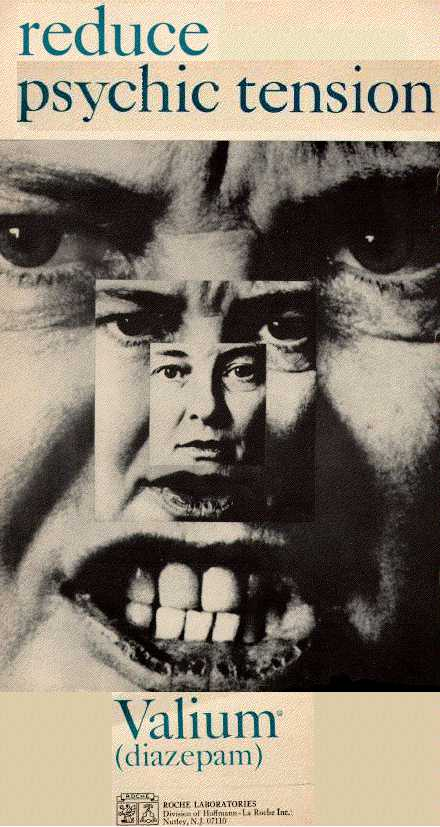
\includegraphics{../images/valium65.jpg}
\end{center}
 \caption{Advertisement for Valium, 1965.  }
\label{fig: valium65}
\end{marginfigure}

From http:\slash \slash faculty.weber.edu\slash ewalker\slash Medicinal\_Chemistry\slash topics\slash Psycho\slash psycho.htm

\end{itemize}

At the same time, we should remember that Medicare and Medicaid were created in 1965, and the health insurance industry was undergoing a simultaneous revolution: 

\begin{itemize}
\item BlueCross 1960:

\end{itemize}

\begin{marginfigure}
 \begin{center}


     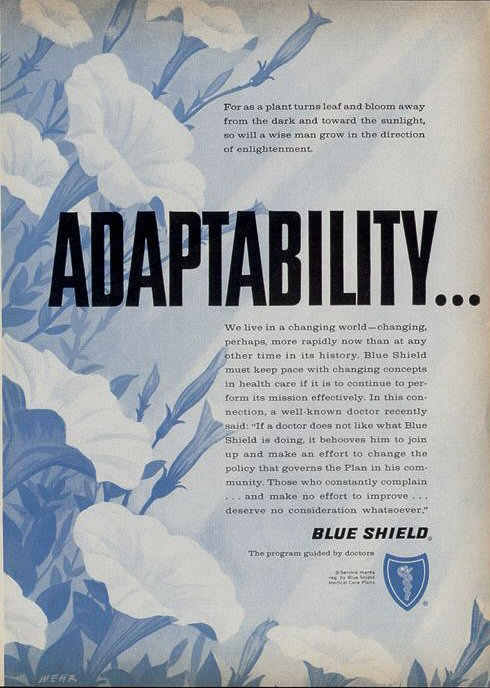
\includegraphics[scale=0.25]{../images/md28530.jpg}
\end{center}
 \caption{Advertisement for Blue Cross, 1960. From http://www.decodog.com/inven/MD/md28530.jpg }
\label{fig: BlueCross}
\end{marginfigure}


\section{Items you might need}
\label{itemsyoumightneed}

\begin{landscape}
\subsection{Credibility Points}
\label{credibilitypoints}
    \begin{tabularx}{\linewidth}{|C{1.75in}|C{1.75in}|C{1.75in}|C{1.75in}|}
      \hline
      \rule{0pt}{1.25in}1 Credibility point & 1 Credibility point & 1 Credibility point & 1 Credibility point \\ \hline
       \rule{0pt}{1.25in}1 Credibility point & 1 Credibility point & 1 Credibility point & 1 Credibility point \\ \hline
       \rule{0pt}{1.25in}1 Credibility point & 1 Credibility point & 1 Credibility point & 1 Credibility point \\ \hline
       \rule{0pt}{1.25in}1 Credibility point & 1 Credibility point & 1 Credibility point & 1 Credibility point  \\ \hline
\label{sample: credibilitypoints}
    \end{tabularx}

  \pagebreak

\subsection{APA positions menu}
\label{apapositionsmenu}

    \noindent
  \begin{longtable}[!t]{ | P{7cm} | P{2cm}  | } \hline
\tahead{Position}&\tahead{Cost} \\ \hline 
Vice-President of the APA& \\ \hline
Member of the Board &  \\ \hline
Chair, Research Committee &  \\ \hline
Chair, Nomenclature Committee &  \\ \hline
Chair, Program Committee &  \\ \hline
\caption{Credibility costs for service to the APA}
\label{sample: credibilitypointsmenu}   
\end{longtable}   
\end{landscape}  
  \pagebreak


\subsection{Labs \slash  possible research proposals}
\label{labspossibleresearchproposals}

Various students should be tasked with presenting proposals for research to the research committee, conducting that research if it is chosen, and presenting the findings at the following conference. Not everything proposed can be carried out in an undergraduate classroom. Where it is impossible, the instructor should distribute the actual paper for evaluation \emph{as if} it had been carried out. The instructors is, of course, encouraged to use classroom activities with which he or she is familiar. 

I've pulled a number of experiments from the APA's \emph{Activities Handbook for the Teaching of Psychology} v. 1--4 that correspond to many of the topics the class will be discussing. They are listed here, and attached as PDFs at the end of this document, if you do not have access to the \emph{Handbooks}. The characters listed here are \emph{suggestions}. The instructor should distribute these as he or she sees fit.

 \begin{longtable}[!t]{ | P{7cm} | P{2.5cm} |   P{3cm} |}
\hline
\tahead{Title, author}&\tahead{Location in APA Handbooks}&\tahead{Suggested character, conference}\\ \hline
Accuracy of Observation, Paul J. Woods&v. 1,\#2&Tyler or Anastasi 1971\\
Operant Conditioning: Role in Human Behavior, Edward Stork&v. 1,\#23&Harlow\\
Operant Conditioning Demonstration, Patricia Keith-Speigel&v. 1,\#24&
Harlow or Hooker\\
Defense Mechanisms, Jack J Greider&v. 1,\#75&Spiegel\\
To Sleep, Perchance to Dream, Ludy T. Benjamin, Jr.&v. 1,\#80&Marmor\\
Mental Illness, James M. Gardner&v. 1,\#81&Lief or Fryer\\
JAWS: Demonstrating Classical Conditioning, Randolph A Smith&v. 2,\#19&Harlow or Hooker\\
Human Operant Conditioning, John K. Bare&v. 2,\#20&Harlow or Hooker\\
Bringing the Clinic Into the Undergraduate Classroom, David M. Young&v. 3,\#45&Someone on the Spitzer Task force, 1974-1975\\
Discovering the Relationship Between Operational Definitions and Interobserver Reliability, Angela H. Becker&v. 4,\#15&Could be instead of Spitzer, 1973, or in combination\\
Information Processing Capacity: A Visual Demonstration of the Magical Number Seven, Fairfid M. Caudle&v. 4,\#43&Marr or Miller\\
The Role of Prior Information in Dream Analysis, Douglas A. Bernstein&v.. 4,\#80&Marmor, after his 1972-1973\\ \hline

\caption{Possible lab activities}
\label{table: labs}
\end{longtable}

\pagebreak 

These are provided to the instructor in case the students fail to come through on research design. They can either be handed to the relevant student to inspire creativity, or “submitted” to the research committee by a mysterious non-player character.

\newpage

\subsection{Emotional responses in a human child.}
\label{emotionalresponsesinahumanchild.}

\subsubsection{Background:}
\label{background:}

Many psychologists--Freud included--have held, with little evidence in support, that the human mind is built on a variety of instincts, such as self-preservation, sexual activity, etc. Emotional responses to fearful stimuli, such as rats and spiders, is commonly considered to be innate, possibly as a result of evolutionary pressures to avoid infectious or poisonous creatures.  This experiment seeks to condition a fear-response in a human infant, thus establishing that there is no need for theoretical innate entities in our explanation of emotion in humans.

\subsubsection{Rationale:}
\label{rationale:}

The success of Pavlov's work conditioning reflex responses to novel stimuli in canines has shown that behaviors previously believed to be instinctual are likely to have resulted from conditioning. The current experiment seeks to determine if that insight can be extended to humans, by conditioning a emotional response in a child—fear—that is widely believed to be instinctual. Demonstrating that these reflexes can appear without appeal to `instinct' or `adaptation' undermines the need for theoretically innate entities in our understanding of human behavior.

\subsubsection{Experimental Design:}
\label{experimentaldesign:}

A child of a single destitute mother, currently employed as a wet nurse at a local hospital (Hopkins), has been recruited for the experiment. Given the nature of his mother's employment, the child is familiar with the clinical setting of a hospital, and hence an ideal subject for this experimental protocol. Previous work with this subject at the age of 8 months has demonstrated that he exhibits fear-like responses to loud sounds: the experimenter stood behind the subject, outside of eye sight and struck a steel bar with a hammer. On the first presentation, the subject startled and raised his hands. On the second, he began to tremble. On the third, he cried and seemed to be having a fit.

The experimenter proposes the following:

\begin{quote}

At 9 months of age, we will present the subject with (randomly): a white rat, a rabbit, a dog, a monkey, with masks with and without hair, cotton wool, and burning newspapers. Given the child's upbringing, it is unlikely that he has ever encountered any of these objects before.  We expect him to have no emotional response to any of them, but if he responds, that object will be removed from the study before proceeding.

At the age of 11 months, one of the objects will be presented to him again. When he moves towards contact with the object, the experimenter will make the loud noise already established as causing a fear reaction.  Each movement towards the stimulus object will cause another loud noise stimulus.  Once the fear reaction is well conditioned, the experimenter will present the subject with the fear-conditioned object and record the response.  The child's reaction than will be compared with other similarly-aged children's reaction for typicality of fear-reactions in children.

The fear-conditioned object will be reintroduced over the subsequent weeks and months at regular intervals to determine the persistence of the conditioned response. 
\end{quote}

\subsubsection{Significance and Contribution}
\label{significanceandcontribution}

This research has the potential to experimentally confirm or deny the commonly held belief that the fear response is innate, or at least instinctual. Pavlov's experiments with classical conditioning in dogs has shown that reflexes that were previously believed to be instinctual—such as salivation—could be conditioned in response to novel stimuli. If Pavlov's approach is to be applied to humans, it is incumbent that psychologists determine the existence and nature of human instinctual reactions, and if they can be conditioned like those of the canine.

\subsubsection{References}
\label{references}

Pavlov, I. P. (1927). Conditioned Reflexes: An Investigation of the Physiological Activity of the Cerebral Cortex.


\newpage

\subsection{Mental rotation of three-dimensional objects}
\label{mentalrotationofthree-dimensionalobjects}

\subsubsection{Background:}
\label{background:}

Mentally rotating 3-dimensional objects is one indicator of spatial reasoning in humans. And it is one that is tempting to explain in terms of internal mental imagery. The `cognitive hypothesis' holds that in order to solve mental rotation problems, a cognitive representation of the presented object must be rotated in the mind before an identification can be made - and it is that hypothesis that we wish to test here.

\subsubsection{Rationale:}
\label{rationale:}

When asked to match three-dimensional objects presented in two-dimensional format, individuals report imagining the object in three-dimensions and rotating them mentally to test against the other possibilities. Introspective reports are, of course, notoriously difficult to address in a scientific way, but that does not mean that we cannot study the phenomenon. If individuals are manipulating mental representations, we would expect a measurable difference in reaction time given a matching task.

\subsubsection{Experimental Design:}
\label{experimentaldesign:}

A number of adult subjects (the size of the class) will presented with pairs of two-dimensional line drawings of three-dimensional blocks. Each subject will be asked to indicate as quickly as possible if the two were drawings of the same object rotated in space or different objects. Half of the experimental set will be rotated versions of the same object, the other half not. They will be presented to the subjects in random order. The time it takes to respond will be measured using computer software. We hypothesize that the amount of time necessary to respond will be correlated with the angle of rotation of the two objects, thus establishing the cognitive hypothesis.

The materials are available on the APA website: http:\slash \slash opl.apa.org\slash Experiments\slash About\slash AboutMentalRotation.aspx Your gamemaster will need to set up an account here: http:\slash \slash opl.apa.org\slash Main.aspx.

\subsubsection{Significance and Contribution}
\label{significanceandcontribution}

This research has the potential to discover observable data that is consistent with the introspective reports of individuals. 

\newpage

\subsection{On Being Sane in Insane Places}
\label{onbeingsaneininsaneplaces}

\subsubsection{Background}
\label{background}

However much mental health practitioners may be personally convinced that we can tell the normal from the abnormal, the evidence is simply not compelling. It is commonplace, for example, to read about murder trials wherein eminent psychiatrists for the defense are contradicted by equally eminent psychiatrists for the prosecution on the matter of the defendant's sanity. More generally, there are a great deal of conflicting data on the reliability, utility, and meaning of such terms as “sanity,” “insanity,” “mental illness” and “schizophrenia.” Finally, as early as 1934, Ruth Benedict suggested that normality and abnormality are not universal. What is viewed as normal in one culture may be seen as quite aberrant in another.

\subsubsection{Rationale}
\label{rationale}

How do we know precisely what constitutes “normality” or mental illness? Conventional wisdom suggests that specially trained professionals have the ability to make resolably accurate diagnoses. In this research, however, we intend to challenge that assumption. What is—and what is not-- “normal” may have to do with the labels that are applied to people in particular settings.

\subsubsection{Experimental Design}
\label{experimentaldesign}

Eight sane people, of varied backgrounds, will gain secret admission to 12 different hospitals, from varied geographical regions of the United States. Their diagnostic experiences will constitute the data of the of the study. The `pseudopatients' will call the hospital for an appointment, complaining of `hearing voices.' When asked what the voices said, they will reply that it was unclear, but that they were `empty,' `hollow,' and `thud.' The pseudopatients will report that voices were unfamiliar and in the same gender as the pseudopatient. After admission to the psychiatric ward, the pseudopatient will cease simulating symptoms of abnormality. 

The amount of time it takes for the pseudopatient to be released, along with any diagnoses and treatments, will be recorded.

\subsubsection{Significance and Contributions}
\label{significanceandcontributions}

This study provides and opportunity to test the reliability of psychiatric diagnosis in the `real world,' rather than the controlled environment of a university lab. The hospital environment imposes a special environment on its members in which the actions of a normal person could be misinterpreted as `insane' or `abnormal.' This study will determine the extent of that influence on psychiatric diagnosis.

\subsubsection{Works Cited}
\label{workscited}

R. Benedict, J. Gen. Psychol., 10 (1934), 59.

\newpage

\subsection{Adjustment of Homosexual and Heterosexual Women}
\label{adjustmentofhomosexualandheterosexualwomen}

Background The traditional psychiatric belief that homosexual men are emotionally unstable has recently been challenged by Evelyn Hooker's study of non-prisoner non-patient homosexual men. There have been a few similar studies on women. The contention that homosexual women are neurotic has typically been voiced by clinicians reporting on their own patients. One exception is the recent psychometric investigation by Kenyon (1968) who studied a non-clinical group of English homosexual women, and concluded that they were higher in neuroticism than a comparison group of heterosexuals. In contrast to the `illness' notion of homosexuality, the authors of three psychometric studies dealing with non-clinical homosexuals and heterosexuals reported that heterosexual women were not better adjusted than homosexuals. (Armon, 1960; Freedman, 1968;

\subsubsection{Rationale}
\label{rationale}

The paucity of research in this area is exemplified by the fact that a total of only four studies, noted above, have been found to date. Even the clinical literature, which is replete with case studies and therapeutic discussions concerning male homosexuality, is strikingly sparse in the area of lesbianism. The present study is proposed to add to the small body of data we now have on the adjustment of homosexual versus heterosexual women.

\subsubsection{Experimental Design}
\label{experimentaldesign}

Working with the leadership of the New York branch of the Daughters of Bilitis, a questionnaire will be sent out to recruit members for the study. And additional questionnaire will be distributed through a popular homophile bookstore in Greenwich Village, New York. And equivalent number of heterosexual women will be recruited from the undergraduate and graduate population of local colleges and universities.

Several different instruments will be used to measure the overall psychological adjustment of the participants, including Scheier and Cattal's Neuroticism Scale Questionnaire (NSQ) (1961) tests of Alienation and Trust (Struening \& Richardson, 1965), Goal Directedness, Self-Acceptance and Sense of Self (Dignan, 1965), Dependency (Comry, 1964), Nurturance (Harvey et al. 1966) and Neuroticism (MacGuire 1966). The Crowne and Marlow Social Desirability Scale (1960) will also be used. The differences on these measures between the homosexual and heterosexual women will be compared to test the `illness' model of homosexuality in women.

\subsubsection{Significance and Contribution}
\label{significanceandcontribution}

Recent interest in and discussions of the `illness' model of male homosexuality have almost completely ignored the parallel issues for homosexual women. This study is a small step towards closing that gap.

\subsubsection{Works Cited.}
\label{workscited.}

Armon, V. (1960) “Some personality variables in overt female homosexuality.” Journal of Protective Techniques, 24, 292--309

Freedman, M.J. (1968) “Homosexuality amoung women and psychological adjustment.” Dissertation Abstracts, 28, 4294B.

Hopkins, J.H. (1969). “The lesbian personality” British Journal of Psychiatry, 115, 1433--6

Kenyon, F.E. (1968). “Studies in female homosexuality: IV. Social and psychiatric aspects.” British Journal of Psychiatry, 114, 1337--50.
Psychometric Tests

Scheier, I. H. \& Cattell, R.B. (1961). The Neuroticism Scale Questionnaire, Champaign, Ill: Institute for Personality and Ability Testing

Struening, E.I. \& Richardson, A.H. (1965). “A factor analytic exploration of the alienation, anomia and authoritarian domain.” American Sociological Review, 30, 768--78.

Dignan, M.H. (1965). “Ego identity and maternal identification” Journal of Personality and Social Psychology 1, 476--83

Comry, A.L. (1964). “Personality factors compulsion, dependence hostility and neuroticism.” Educational and Psychological Measurement, 24, 75--84

Harvey, O.J., Prather, M.S. White, J. and Alter, R.D. (1966).”'Teachers' belief systems and preschool atmospheres” Journal of Educational Psychology 57, 373--81

McGuire, R.G. (1966). “An inquiry into attitudes and value systems of a minority group.” Unpublished Doctoral Dissertation, NYU

Crowne, D.P. \& Marlowe, D. (1960). “A new scale of social desirability independent of psychopathology.” Journal of Consulting Psychology, 24, 349--54

\newpage

\subsection{A Re-analysis of the Reliability of Psychiatric Diagnosis}
\label{are-analysisofthereliabilityofpsychiatricdiagnosis}

\subsubsection{Introduction}
\label{introduction}

Classification systems such as diagnosis have two primary properties, reliability and validity. Reliability refers to the consistency with which subjects are classified; validity, to the utility of the system for its various purposes. In the case of psychiatric diagnosis, the purposes of the classification system are communication about clinical features, aetiology, course of illness and treatment. A necessary constraint on the validity of the system is its reliability. There is no guarantee that a reliable system is valid, but assuredly an unreliable system must be invalid.

\subsubsection{Background}
\label{background}

Studies of the reliability of psychiatric diagnosis provide information on the upper limits of its validity. This study will consider some of the difficulties in appraising diagnostic reliability, offers a re-analysis of the available data from the literature, and suggests a possible course of action to improve psychiatric diagnosis.

\subsubsection{Rationale}
\label{rationale}

Zubin (1967) reviewed the major studies of reliability of psychiatric diagnosis performed until 1966. He noted that diagnostic reliability is referred to in three different ways: agreement between independent diagnosticians examining the same patients, stability in diagnosis over time, and similarity in diagnostic frequencies for comparable samples. It is the first sense—interjudge agreement—that is fundamental.

Recent studies of interjudge agreement of psychiatric (Schmidt and Fonda, 1956; Kreitman, 1961; Beck et al., 1962; Sandifer et al., 1964) report on agreement as to the presence of absence of a diagnosis, but they neglect to consider the rate at which diagnoses are made.

Cohen (1960) has recently developed a statistical measure (called `kappa') of interjudge agreement that incorrporates a correction for chance agreement. This study proposes to recalculate the reliability of psychiatric diagnosis from these studies based on Cohen's Kappa.

\subsubsection{Experimental Design}
\label{experimentaldesign}

The study will use existing data, culled from five recent papers measuring the interjudge agreement of psychiatric diagnosis.

\subsubsection{Significance and Contributions}
\label{significanceandcontributions}

There is little doubt that the reliability of psychiatric diagnosis is being questioned at this time. If the presumed agreement of previous work depends merely on the rate of chance agreement, psychiatry must reevaluate it classification system immediately.

\subsubsection{Works Cited}
\label{workscited}

Cohen, J. (1960) “A coefficient of agreement for nominal scales.” Educ. Psychol. Measmt., 20, 37--46.

Beck, A.T., Ward, C.H., Mendelson, M., Mock, J.E., \& Erbaugh, J.K. (1962). “Reliability of psychiatric diagnosis: 2. A study of consistency of clinical judgments and ratings.” Amer. J. Psychiat., 119, 351--7

Sandifer, M.G., Pettus, C. \& Quade, D. (1964). “A study of psychiatric diagnosis.” J nerv. ment. Dis., 139, 350--6

Kreitman, N. (1961) “The reliability of psychiatric diagnosis” J. ment. Sci. 107, 876--86.

Schmidt, H.). \& Fonda, C.P. (1956). “The reliability of Psychiatric Diagnosis: A new look” J. abnor. soc., Psychol. 52, 262--7

Zubin J. (1967) “Classification of the behavior disorders” in Annual Review of Psychology (eds. P. R. Farnsworth \& O. McNemar). Palo Alto, California, Annual Reviews, pp. 373--406.

\newpage

\subsection{Interpersonal Dynamics in a Simulated Prison}
\label{interpersonaldynamicsinasimulatedprison}

\subsubsection{Background}
\label{background}

After he had spent four years in a Siberian prison the great Russian novelist Dostoevsky commented, surprisingly, that his time in prison had created in him a deep optimism about the ultimate future of mankind because, as he put it, if man could survive the horrors of prison life he must surely be a “creature who could withstand anything.” In the century which has passed since Dostoevsky’s imprisonment, little has changed to render the main thrust of his statement less relevant. Although we have passed through periods of enlightened humanitarian reform, in which physical conditions within prisons have improved somewhat and the rhetoric of rehabilitation has replaced the language of punitive incarceration., the social institution of prison has continued to fail. On purely pragmatic grounds, there is substantial evidence that prisons neither “rehabilitate” nor act as deterrent to future crime—in America, recidivism rates upwards of 75\% speak quite decisively to these criteria. On humanitarian grounds as well prisons have failed: our mass media are increasingly filled with accounts of atrocities committed daily, man against man, in reaction to the penal system or in the name of it. The prison undeniably creates, almost to the point of cliché, an intense hatred and disrespect in most inmates for the authority and the established order ot society into which they will eventually return. And the toll which it takes on the deterioration of human spirit for those who must administer it, as well as for those upon whom it is inflicted is incalculable.

\subsubsection{Rationale}
\label{rationale}

Attempts to provide an explanation of the deplorable condition of our penal system and its dehumanizing effects upon prisoners and guards, often focus upon what might be called the \emph{dispositional hypothesis}. While this explanation is rare expressed explicitly, it is central to a prevalent non-conscious ideology: that the state of the social institution of the prison is due to the “nature” of the people who administer it, or the “nature” of the people who populate it, or both. That is, a major contributing cause to despicable conditions, violence, brutality, dehumanization and degradation existing with any prison can be traced to some innate or acquired characteristic of the correctional and inmate population.

The dispositional hypothesis has been embraced by the proponents of the prison \emph{status quo} (blaming conditions on the evil in the prisoners), as well as by its critics (attributing the evil to guards and staff with their evil motives and deficient personality structures). A critical evaluation of the dispositional hypothesis cannot be made directly through observation in existing prison settings, since such naturalistic observation necessarily confounds the acute effects of the environment with the chronic characteristics of the inmate and guard populations. TO separate the effects of the prison environment per se from those attributable to a priori dispositions of its inhabitants requires a research strategy in which a “new” prison is constructed, comparable in its fundamental social-psychological milieu to existing prison systems, bt entirely populated by individuals whoa re undifferentiated in all essential dimensions form the rest of society.

\subsubsection{Experimental Design}
\label{experimentaldesign}

Interpersonal dynamics in a prison environment are to be studied experimentally by designing a functional simulation of a prison in which subjects role-pay prisoners and guards for an extended period of time. To assess the power of the social forces on the emergent behavior in this situation, alternative explanations in terms of pre-existing dispositions are to be eliminated through subject selection. A homogeneous, “normal” sample is to be chosen after extensive interviewing and diagnostic testing of a large group of volunteer male college students. Half of the subjects are to be randomly assigned to role-play prison guards for eight hours each day, while the others role-play prisoners incarcerated for nearly one fill week. Neither group will receive any specific training in these roles. The primary investigator will role-play the prison warden, and consultants from the real prison population (both prisoners and prison officials) will be recruited to assist in the planning and implementation of the prison environment.

Continuous, direct observation of behavioral interactions will be supplemented by video-taped recording, questionnaires, self-report scales and interviews. All these data sources are likely to converge on the conclusion that this simulated prison will develop into a psychologically compelling prison environment.

\subsubsection{Significance and Contributions}
\label{significanceandcontributions}

The authors believe that this demonstration will reveal new dimensions in the social psychology of imprisonment worth pursuing in future research, In addition, this research will provide a paradigm and information base for studying alternatives to existing guard training, as well as for questioning the basic operating principles o which penal institutions rest. There is great need today for prison reforms that recognize the dignity and humanity of both prisoners and guards whoa re constantly forced into one of the most intimate and potentially deadly encounters known to man. This study has the potential to inform those reforms.

\subsubsection{Works Cited}
\label{workscited}

\newpage

\subsection{Small World}
\label{smallworld}

\subsubsection{Background}
\label{background}

\subsubsection{Rationale}
\label{rationale}

\subsubsection{Experimental Design}
\label{experimentaldesign}

\subsubsection{Significance and Contributions}
\label{significanceandcontributions}

\subsubsection{Works Cited}
\label{workscited}

\newpage

\subsection{Learning Objectives}
\label{learningobjectives}

In many ways, this is not a game about Psychology or Psychiatry, it is a game about the Philosophy of Science. This shouldn't really be surprising, as the history of the Psychology and Psychiatry is intimately linked to the history of the Philosophy of Science. Arguments made by Wundt, Freud, Watson, Hull Skinner and Miller all rely heavily on claims regarding what is or is not a legitimate scientific claim.\footnote{See, e.g. Wundt (1902, pg 5--6) Freud \_\_\_\_, Watson (Mathematical paper), Skinner \_\_\_\_\_, Hull, (1935), Miller (citing Suppes)} This issues has not disappeared from undergraduate Psychological classroom either. The APA's guidelines for the Undergraduate Major in Psychology, published 2007, lists 10 learning outcomes for a major. The first is:

\begin{apatextbox}{Excerpt from APA Guidelines for an Undergraduate Major in Psychology, 2007}

\textbf{Goal 1: Knowledge Base of Psychology}

\begin{quote}

Demonstrate familiarity with the major concepts, theoretical perspectives, empirical findings, and historical trends in psychology
\end{quote}

\textbf{Suggested Learning Outcomes}

\begin{quote}

1.1. Characterize the nature of psychology as a discipline

\begin{quote}

a) Explain why psychology is a science.

b) Identify and explain the primary objectives of psychology: describing, understanding, predicting, and controlling behavior and mental processes.

c) Compare and contrast the assumptions and methods of psychology with those of other disciplines

d) Describe the contributions of psychology perspectives to interdisciplinary collaboration.
\end{quote}
\end{quote}

\end{apatextbox}

If the reader compares to the definitions offered by the various historical figures in the ‘\fullref{briefhistoryoftheapa}’ in the gamebook, you will no doubt recognize the theoretical pluralism embodied in the APA's statements. These guidelines were superseded by the more prescriptive ‘Version 2.0’ in 2013, but the same themes reappear:

\begin{apatextbox}{Excerpt from APA Guidelines for an Undergraduate Major in Psychology 2.0, 2013}

\textbf{Goal 1: Knowledge Base in Psychology}

\begin{quote}

1.1 Describe key concepts, principles, and overarching themes in psychology.

\begin{quote}

1.1a Use basic psychological terminology, concepts and theories in psychology to explain behavior and mental processes.

1.1b Explain why psychology is a science with the primary objectives of describing, understanding, predicting and controlling behavior and mental processes.

1.1c Interpret behavior and mental processes at an appropriate level of complexity.

1.1d Recognize the power of the context in shaping conclusions about individual behavior.

1.1e Identify fields other than psychology that address behavioral concerns.
\end{quote}
\end{quote}


\end{apatextbox}

Version 2.0 instrumentalizes the ‘nature of psychology as a discipline’ into the measurable phrase ``use basic psychological terminology, concepts and theories.'' It is also notable that the phrase “and mental processes” appears in three of the subpoints (1.1a, 1.1b and 1.1c), rather than just one (b). One might be tempted to assert that behaviorism is well and truly dead in Psychology. 

My main for quoting this document is, however, 2007 (a) and 2013 (1.1b).

The question \emph{if} psychology is a science is a question of demarcation – the classic issue in the Philosophy of Science. But answering \emph{why} psychology is a science assumes a affirmative answer to the demarcation problem, and hence, a particular view in the Philosophy of Science. 

For example, Wundt charged Hebart with non-scientific investigations into introspection,\footnote{Wundt, 1902, pg. 5--10} because Hebart did not adequately control the environment. Watson charged that McDougall's notion of behaviors having a `purpose' was non-scientific,\footnote{Watson 1929, pg. 25--6 “The Behaviorist finds no scientific evidence for the existence of any vitalistic principle, such, for example, as Prof. MacDougall's 'purpose{\ldots} {\ldots}There are many things we cannot explain in behavior just as there are many things we cannot explain in physics and chemistry, but where objectively verifiable experimentation ends, hypothesis, and later theory, begin.”} because McDougall did not follow strict verificationism in the philosophy of science. When Hull charged that Tolman's explanations were unscientific because they positing internal entities, he did so by citing Newton\footnote{Newton, the critic would note, posited `force', an invisible entity that was criticized at the time as an `occult' power.} (1935). Miller and Chomsky rejected Skinner's arguments by citing Philosophers of Science such as Patrick Suppes, who contend that the history of science shows that scientists do posit internal entities, if they can modeled mathematically.

\subsubsection{Textbooks: A brief review of introductory textbooks in psychology demonstrates that the current crop of answers here is not good-}
\label{textbooks:abriefreviewofintroductorytextbooksinpsychologydemonstratesthatthecurrentcropofanswershereisnotgood-}

Most \emph{Introduction to Psychology} textbooks address Goal 1 in Chapter 1. The all include a brief historical overview, and all note Wundt, James, Freud and Pavlov. 

\begin{longtable}[!t]{ | P{2cm} | P{3cm} | P{6cm} | P{3cm} | }
\hline
\tahead{Book} & \tahead{Def. Of ‘Science’} & \tahead{Historical highlights (I.e. Section heads)} & \tahead{other notable items}  \\ \hline
~\citep{Lilienfeld:2014ws}&”A systematic \emph{approach} to evidence” (p.8)&Early History (27-29), Structuralism (30), Functionalism (30), Behaviorism (30-31), Cognitivism(31) and Psychoanalysis (31-32)&Significant section on pseudoscience (p. 12-26) \\ \hline
~\citep{Cacioppo:2018we}&”a special way of learning about reality through systematic observation and experimentation.” (p. 36) &Greek philosophers, British empiricists, ancient physicians, 17th and 18th century natural scientists, Helmholtz (all 6-10), Wundt (11-12), Gestalt (12), James, (12-14), Freud (14) \& Humanistic Psychology (15), Behaviorists and Cognitive Revolution (16-21)  & Defines ‘psychology’ as ‘science of mind’ rather than ‘science of behavior and mental processes’ (p. 5)\\ \hline
~\citep{Cervone:2015ud}& ‘scientific methods refers to a broad array of procedures through which scientists obtain information about the world’ (p. 9)---Collect evidence, record observations systematically, record how observations were made.& Aristotle \& Buddha (20-22) Locke \& Kant (22-24), Wundt (24-25), James (25-26), Structuralism \& Functionalism (27), Psychoanalysis, Behaviorism (28), Humanistic (28-29), Information Processing and the Cognitive Revolution (29-30)& \\ \hline
~\citep{Gazzaniga:2018tq}& ‘psychology: the study through research of mind, brain and behavior’--“gain accurate knowledge about behavior and mental processes only by observing the world and measuring aspects of it” (p. 30)&Descartes (p. 10-11), Wundt (11-12), Structuralism (12), Functionalism (12), Evolution, Adaptation and Behavior (13), Psychoanalytic Approach (14), Behaviorism (15), Gestalt (15-16), Humanistic (16), Cognitivism (16)& Additional definition of ‘scientific method’ that combines method with goals. \\ \hline
~\citep{Hockenbury:2014ws}&The scientific method is a set of assumptions, attitudes , and procedures that guides all scientists, including psychologists, in conducting research (16) -- empirical evidence: “Verifiable evidence that is based upon objective observation, measurement and/or experimentation.” (16)&Influence of Philosophy and Physiology (3-4), Wundt (4), Titchener (4-5), James (5-6), Freud (7-8), Watson (8), Rogers (9)& \\ \hline
~\citep{Myers:2015ws}&”less a set of finding than a way of asking and answering questions” (5)&Wundt (2), Structuralism and Functionalism (2-3), First Women in Psychology (3-4),Behaviorism (4), Freudian Psychology (5), Humanistic Psychology (5), Cognitive Revolution (5)& \\ \hline
~\citep{Zimbardo:2012uz}&”based on objective, verifiable evidence---not just the opinions of experts and authorities, as we often find in non-scientific fields” (4) &Separation of Mind and Body and the Modern Biological Perspective (Descartes (12-13)), The Founding of Scientific Psychology and the Modern Cognitive Perspective (Wundt (13-14), Structuralism (Titchener) (14), James (14-15), Cognitive (15-16)), The Behavioral Perspective (16-17), The Whole-Person Perspective (17-19), The Developmental Perspective, The Sociocultural Perspective& “Perspective” approach is unique in the set of textbooks reviewed.\\ \hline
~\citep{Rathus:2012uz}&”Psychology, like other sciences, seeks to describe, explain, predict, and control the events it studies... ...behavior and mental processes.” (4)& Aristotle(8-9), Structuralism - Wundt (9), Functionalism - James (9-10), Behaviorism (10), Gestalt (10-11), Psychoanalysis (11-12)& \\ \hline
\caption{Timeline of critical events}
\label{table: timeline}
\end{longtable}

When one reviews these offerings, one is struct by the lack of variation. All cite the same historical movements---including, somewhat surprisingly, humanistic psychology. They \emph{all} define science as a method or procedure, and all reject the notion that science is a body of knowledge to be memorized. This cannot be random.

Moreover, the idea that science can be distinguished from non-science or pseudoscience based on method alone is highly questionable. Ptolemic astronomy based its work on careful observation, and applied the rigorous methods of mathematics in order to describe and predict the movements of the heavens. So does astrology. On the other side of the dialectic, there is little in relativistic physics or quantum mechanics that is observable or was subject to experiment \emph{before} it was accepted as scientific. 

So neither way is the view articulated by these textbooks correct---there are non-scientific endeavors that fit the methodology-based demarcation, and there are scientific endeavors that do not. Simply speaking, one cannot demarcate science from non-science using methodology alone. 

We are in dire need of a richer, more complete approach to introducing the scientific history of Psychology.

\subsubsection{Learning Objectives of the Game}
\label{learningobjectivesofthegame}

At the completion of this game, the students will be able to:

\begin{itemize}
\item Recognize that the historical contingency of the concepts, principles and overarching themes that define and distinguish of our contemporary disciplines of the mind.

\item Identify and respond to historical examples where debates about evidence shift into debates whether or not the evidence is scientific---i.e., about the philosophy of science, and the legitimacy of evidence. (See examples in XX[ Peter Bradley, 7\slash 23\slash 18, 4:44 PM])

\item Demonstrate, using actual examples from historical psychology, a more sophisticated understanding of the process of scientific inquiry than the simplistic experimental model. 

\begin{itemize}
\item Understand the concept of a ‘paradigm’ as Kuhn originally meant it: as a ‘model’ experiment that defines an era of a discipline or a scientific culture.

\item Distinguish between observational studies, experimental interventions and modeling, and the scientific value of each.

\item Apply their understanding of paradigm cases like Newton’s \emph{Experimentum Crucis}, and Hermann Ebbinghaus’ memory experiments as \emph{the} paradigm of experimental psychology, to judge the validity of new and novel research proposals.

\item Recognize and manipulate the logical structure of scientific proposals (i.e. The H-D method) and recognize that the reasoning of real, historical scientists does not often follow this ideal.

\item Identify potential confounding variables in basic experimental design, and suggest ways those variables may be controlled. 

\item Identify the strengths and weaknesses of non-experimental social science methods, specifically observational research (both naturalistic and participant-observation) and modeling; and apply this analysis to real-word cases (~\citep{Rosenhan:1973uq}, ~\citep{Haney:1973wf}, e.g.).

\end{itemize}

\item Demonstrate a working knowledge of the intellectual ‘environment’ that gave rise to behaviorism and psychoanalysis.

\item Engage with primary sources in the history of psychology.

\item Demonstrate a working knowledge of the major distinctions in the study of the mind: psychodynamic, behavioristic and cognitive,\footnote{We cover---very briefly---James’ functionalism and Titchener’s structuralism, though not quite using those names, in the Game book, section \fullref{briefhistoryoftheconceptofpsychology}. These views are not given voice in the game, as contemporary parallels tend to reside in Philosophy departments, not psychology.} including being able to correctly categorize major views \slash  works, and discuss the complexity of cases on the margins (i.e. Tolman, Bandura)

\item Appreciate the social impact taxonomies and labels can have on others, and the social significance thereof.

\end{itemize}

\subsection{Conceptual issues at stake}
\label{conceptualissuesatstake}

Many of the issues raised in the course of the game are appropriately philosophical. While we've instructed the students to focus on the evidence, and its relationship with the claims asserted, one is often forced to notice how few of the great conflicts in the history of psychology and psychiatry are actually about the quality of the evidence presented. The conflicts are, most frequently, actually about whether the evidence in question can be considered `scientific.' 

The APA guidelines cited above do not report \emph{what} the key terminology, concepts and theories are---but they do cite a three instruments to assess whether or not students are meeting these goals. The Psychology Area Concentration Achievement Test has 12 content areas:

\begin{itemize}
\item Abnormal

\item Animal Learning and Motivation

\item Clinical and Counseling

\item Developmental

\item Experimental Design

\item History and Systems

\item Human learning and cognition

\item Personality

\item Physiological

\item Sensation and Perception

\item Social

\item Statistics

\end{itemize}

I've noted where in the games these issues arise.

Some of these issues that will make an appearance in the game are:

\begin{itemize}
\item Is mental illness a disorder of an individual or a society? (i.e. are the entities studied in psychology individual humans or human societies?) -Clark, Albee, Szasz

\item Is medical model an appropriate model for the classification, diagnostic criteria and treatment of mental disorders? Szasz, Albee v. Spitzer

\item Related: Should mental disorders be classified in terms of their causes (etiology), or their symptoms? (psychoanalysts v. Spitzer)

\item Are mental health norms defined in terms of statistical frequency of a given behavior in the population, or ideals of human behavior? (Anastasi v. Bieber)

\item Is modeling \slash  abductive reasoning a scientific method, or is science limited to explanations of observable behavior in terms of observable behavior? (cognitivists v. behaviorists)

\item What are the responsibilities of scientists who study humans and human societies for social advocacy? (Chomsky, Skinner, Albee, Clark v. Tyler, Bieber)

\end{itemize}

\subsubsection{Philosophy of Science rearing its ugly head}
\label{philosophyofsciencerearingitsuglyhead}

Well, not ‘ugly’ per se. But still{\ldots}

\subsubsection{Research design}
\label{researchdesign}

I’ve included a ‘textbook’ style section (\fullref{testingcausalclaimsexperimentally}) in the game book that introduces the standard independent variable - dependent variable - controls logic that is included in most research methods in psychology courses. I prefer, of course, to introduce these ideas with real historical examples, as I did in section \fullref{theparadigmaticexperiments}.

I included the digested ‘textbook’ section to give the research committee a quick and dirty heuristic for judging the validity of proposed experiments. But this simplistic approach is largely misguided. There are famous examples from this period that simply don’t fit the model:

\begin{itemize}
\item We know that the IV in Zimbardo’s prison ‘experiment’ is assignment to either ‘prisoner’ or ‘guard’ role, but what is his DV?

\item Milgrim measured the number of hops a letter would take in his ‘small world’ experiment, but what is his manipulation of the IV?

\item Similarly, we know that Rosehan measured the time spent inside a mental health institution, but what was the IV?

\end{itemize}

We want the research committee to raise these kind of questions when these proposals come before the committee. If we taught solely from historical examples, these concerns might not be raised. 

\section{Overview of events and assignments in the game}
\label{overviewofeventsandassignmentsinthegame}

 \begin{longtable}[!t]{ | p{2cm} | p{2cm} | p{2cm} |p{2cm} | p{6cm} |  }
Year\newline
Class&
Presidential address&
Talks (symposia and research reports)&
Proposals&
Research Tasks\\
\multicolumn{5}{ | p{14cm} | }{1971 Washington DC} \\ \hline
A&
G. Miller  “Psychology as a means of promoting human welfare”&
 




Symposium “Psychiatry: Friend or Foe to Homosexuals: A Dialogue,” (J. Fryer, E. Hooker, F. Kameny /  B. Gittings)&

Proposal from J. Marmor / R. Gold to remove homosexuality from next DSM – send to nomenclature (opposed: Bieber / Socarides)&
Presentation of 'Mental Rotation' task - gamemaster\\

B&



&


T. Szasz “The Myth of Mental Illness”\newline
J. Marmor “Limitations of Free Association”&
Proposal from C. Socarides to create task force to sexual deviation (Really 1970 to NY branch, reported in 1972, when it was rejected).\newline
Proposal from J. Spiegel and R. Green to create task force of historical study and literature review of homosexuality in psychology and psychiatry.&
Research Report on 'Mental Rotation' data by Miller\\
\multicolumn{5}{ | p{14cm} | }{1972 Dallas} \\ \hline
A&
Bandura “Behavioral theory and models of man”&





Symposium on the 'medical model' \(T. Szasz, G. Albee\)
\newline
Report from Green and Spiegel on history of homosexuality – responses from Bieber, Marmor&

Proposal to recognize the contributions of Evelyn Hooker \(From Gebhard\)&
Research committee considers Rosehan\\
B&
 




Paper by Spitzer on Feighner Criteria\newline
Paper by Gebhard on the Kinsey report.\newline
Paper by Harlow “Lust, latency and love”&
Proposal from nomenclature to write a new DSM according to description of symptoms, not causes (Opposed: Lief)\newline
Proposal from Hopcke to limit medical care of mentally distressed individuals in hospitals to licensed medical doctors (i.e. psychiatrists)\newline
Counter proposal from Albee to limit the role of psychiatrists to the admission of drugs &
Research Report of Rosehan report by TO BE ASSIGNED\\
\multicolumn{5}{ | p{14cm} | }{1973 Honolulu* \newline
 *(on Gay Pride day in 1973, someone firebombed the 'UpStairs Lounge', a gay club in New Orleans, killing 32 people, 3 of whom were never identified.  The Game Master may wish to distribute the news prior to the APA conference, if he or she wishes to drive home the threat faced by LGBT people in 1973.  See http://www.patheos.com/blogs/friendlyatheist/2013/06/24/remembering-the-upstairs-lounge-the-u-s-a-s-largest-lgbt-massacre-happened-40-years-ago-today/  for a blog-length history, or “Let the Faggots Burn: The UpStairs Lounge Fire” by Johnny Towsend for a book-length history).} \\ \hline
A&
Tyler – on individual differences & their importance for counseling.
&



Bieber / Socarides report\newline
Report from Socarides (rejected) ← challenged by Gold, Spitzer, leading to GayPA meeting (actually 1973)&

Proposal from Marmor condemning Socarides' JAMA paper as nonscientific and a 'monstrous attack on homosexuality.' (opposed Bieber and Socarides, also Bandura, for reasons of academic freedom and professionalism)
Research committee considers Zimbardo
Consider Fordney Settlage, Spitzer\\

\multicolumn{5}{ | p{14cm} | }{Famous GayPA meeting of Spitzer and Gold. They supposedly draft their resolutions overnight.} \\ \hline
B&


 &
Symposium “A Symposium: Should Homosexuality Be in the APA Nomenclature?” (Green, Marmor, Bieber, Gold, Socarides, Spitzer – organized by Kameny / Gittings)&
Proposal for Leona Tyler Principle (opposed: Clark, Chomsky)\newline
Proposal from Gold & Spitzer to remove 'homosexuality' immediately. (Green opposed to vote, not issue)\newline
Proposal to create dissolve nomenclature committee and create “Spitzer Taskforce” (opposed: Hooker)
Research Report of Haney et al. report by Zimbardo (if in game, if not, distribute the paper to the class)\\
\multicolumn{5}{ | p{14cm} | }{1974 Philadelphia} \\ \hline
A&
Clark – on psychology's role for social good / Anastasi – on psychometics&




Symposium on the responsibility of intellectuals – (Chomsky, Clark, Marmor?)\newline
Paper by Smilgram 'obedience'\newline
Paper by H. Lief on genetic hypothesis and diagnostic taxa.&
Proposal from Anastasi to create committee on women in Psych, and the Psych of women (opposed: Szasz)&
Research committee considers Milgram 'small world’\\
B&


&


Spitzer task force open hearings on proposed definition of 'mental illness' (no symposium)&
Proposal from Fryer deem the use of aversion therapy to treat homosexuals as 'immoral' (opposed: Harlow)&

Research Report of Small World (if complete) report by Milgram (if not, postpone to 75). (If Milgram not in game, distribute)\\
\multicolumn{5}{ | p{14cm} | }{1975 Chicago} \\ \hline
A&
Clark / Anastasi / Spiegel – on the DSM-III controversy&



Open discussion / vote of the membership on definition of mental illness.\newline
Zimbardo on the 1968 code of ethics\newline
D. Fordney Settlage on the disparity between psychoanalytic theories of male and female sexuality.\newline
Hopcke on Jungianism and homosexuality&
Proposal from Clark create affirmative action plan in psychology and psychiatry (see proposals section) (opposed: Milgram)&
Research committee considers TO BE ASSIGNED\\
B&

&

Marr on Levels of explanation in psychology \newline
Symposium on 'innateness' (Chomsky / Piaget)&
Proposal to revise APA ethics guidelines in wake of Zimbardo study (research committee)&
Research Report of TO BE ASSIGNED report by TO BE ASSIGNED\\
\hline
\caption{Overview of Game events, by year}
\label{table: overviewbyyear}
\end{longtable}


Table 4: Overview of game events, by year
 Milgrim\footnote{Milgram is the only psychologists of this era for whom I can find documentation of opposition to the affirmative action plan, although it was certainly more widespread. That documentation is, suffice it to say, sparse. It is mentioned once in Blass, T. (2009). The Man Who Shocked The World: The Life and Legacy of Stanley Milgram Public Affairs, p. 201.} note
 \#\#\#\# Overview of assignments, by character
 \begin{longtable}[!t]{ | p{1cm} | p{2cm} | p{6cm} |  p{3cm} |  p{3cm} | }
\hline
Name&
Committee Work&
Paper&
Proposals&
Research\\ \hline
G Albee&
Nomenclature '71-'72 \newline
Board member 'B' '71-'72*&
'Medical Model' – symposium '72&
Parallel medical system for clinical psychology '72&
\\
A. Anastasi&
Program '71-'73&
“On psychometrics” - presidential '74&
Proposal to fix gender-specific language in guidelines (program committee '71)
Women in Psych / Psych of Women '74&
\\
A. Bandura&
VP '71\newline
(Board '71-'73)&
“Behavioral theory and models of man” '72&
'73 – reject Bieber&
\\
I. Bieber /
C. Socarides&
&
Comment on Green / debate Marmor '72\newline
Report on sexual deviation (Freudian) '73
Symposium on nomenclature '73 (both, if in game)&
Propose taskforce '71, report '73\newline
Oppose Marmor & Gold's '71 proposal to remove 302.0 from DSM-II\\
N. Chomsky&
&
“The responsibilities of Intellectuals” - symposium '74 (could be paper)\newline
Debate with Piaget '75&
Oppose L. Tyler principle '73&
\\
K. Clark&
Research '71-'73&
“psychology as a force of social change” - symposium '74 (could be presidential)&
Oppose L. Tyler principle '73\newline
Proposal to create affirmative action plan '75&
\\
D. Fordney Settlage*&
&
Paper critiquing the focus on male sexuality '75&
Propose balance compromise Albee and Hopcke on psych. \newline Practicing in hospitals, but not prescribing drugs. &
Sexual experiences of younger women seeking contraceptives. '73\\
J. Fryer&
&
“I am a homosexual, and a psychiatrist.” - symposium '71&
Proposal to deem the use of aversion therapy as immoral '74&
\\
P. Gebhard&
Program '71-'74&
Summary of the Kinsey report '72&
Honor of E. Hooker '72&
\\
R. Gold*&
&
Symposium on nomenclature '73&
Support Marmor's '71 proposal\newline
Draft proposal with Spitzer '73&
\\
R. Green*&
&
Report on history of homosexuality '72 (with J. Spiegel)
Symposium on nomenclature '73&
Taskforce on the history of homosexuality in Psych '71 (with Spiegel)&
*APA v. 3 45 '74-'75 (Clinic in Ugrad classroom)*\\
H. Harlow&
Board '71&
“Lust, latency and love” - paper '72&
Defend the use of aversion therapy '74&
APA v. 1 \#2 (Operant Conditioning)\\
E. Hooker&
Program '71-'72&
“The mental health of non-patient male homosexuals” - symposium '71&
Oppose dissolution of nomenclature committee.&
\\
R. Hopcke*&
&
Jungian approaches to homosexuality '75&
Support the proposal to limit care of mental illness to MDs&
\\
F. Kameny* / B. Gittings*&
&
“Gay, Proud and Healthy” - symposium '71&
Organize and Chair the 'big' symposium “Should 'homosexuality' be in the DSM-III?' in '73 where Green, Marmor, Bieber, Gold, Socarides, Spitzer should speak.&
Propose Siegelman “Adjustment of homosexual women” 1971\\
H. Lief*&
&
Paper on genetic hypothesis and diagnostic taxa '74&
Oppose Spitzer's nomenclature proposal '72&
\\
J. Marmor&
Research '71-'74&
“Limitations of Free Association” - paper '71\newline
Comment on Green / debate Bieber '72\newline
Symposium on nomenclature '73&
Propose 'homosexuality' be removed from category 302. '71\newline
Propose a condemnation of Socarides' JAMA paper. '73&
APA v. 4 \#80 '73 (Dream Analysis)\\
D. Marr*&
&
'Levels' of explanation paper '75&
&
Propose APA v. 4 \#43 '72 (Magic number 7)\\
S. Milgram*&
Board member ‘A’*&
Summary of obedience experiments / findings '74&
Oppose affirmative action plan - '75&
Propose 'small world' experiment '74\\
G. Miller&
Board '71-'72&
“Psychology as a means of promoting human welfare” - '71&
'72 – reject Bieber&
Present Mental Rotation '71 (Shepard / class data)\\
J. Piaget*&
&
Debate with Chomsky '75&
&
\\
L. Tyler&
Research '71-'72&
“Design for a hopeful psychology” - president '73&
Leona Tyler principle '73&
\\
J. Spiegel&
Nomenclature '71-'74&
Report on history of homosexuality '72 (with R. Green)
Presidential address '75&
Taskforce on the history of homosexuality in Psych '71 (with Green)&
\\
R. Spitzer&
Nomenclature '71-'76&
“The Feighner Criteria” '72\newline
Symposium on nomenclature '73\newline
Open hearing '74 on 'mental illness’&

As nomenclature committee: write DSM according to description of symptoms, not causes '72
AND proposal to disband nomenclature & form Spitzer Taskforce '73\newline

With R. Gold, draft proposal to remove 'homosexuality' immediately in '73
Reliability of psychiatric diagnosis '73\\
T. Szasz&
&
“The myth of mental illness” - paper '71\newline
“Medical Model” -  symposium '72&
Oppose committee on psychology of women '73 (on grounds of reification of the term 'women’)&
\\
P. Zimbardo*&
&
Paper on the ethical problems of Zimbardo '73, \newline and any holes in the APA guidelines. '75&
&
Propose Zimbardo '73 (if character is not used, the proposal should come from the gamemaster)\\ \hline

\caption{Overview of specific assignments, by character}
\label{table: overviewcharacter}
\end{longtable}

Papers in italics are conditional. If not elected, the students should present them as papers.
Research items in italics are NOT included in the character sheet, and can be moved around by the instructor. See Activities section on p. 23.
*Not included in games smaller than 26.

\subsubsection{Overview of elections, by year}
\label{overviewofelectionsbyyear}

 \begin{longtable}[!t]{ | p{1cm} | p{2cm} | p{1cm} |  p{2cm} | p{2cm} | p{2cm} |}
\hline
Year&
VP&
Board-at-large*&
Research (replacing)&
Nomenclature
(replacing)&
Program
(replacing)\\ \hline
1971&
1972 (Bandura)&
A (Milgram)&
&
&
\\
1972&
1973 &
B (Albee)&
(Tyler)&
(Albee)&
(Hooker)\\
1973&
1974&
&
(Clark)&
&
(Anastasi)\\
1974&
1975&
A&
(Marmor)&
(Spiegel)&
(Gebhard)\\
1975&
1976&
B&
(elected 1972)&

(elected 1972)\\ \hline
\caption{Elections to be held each year}
\label{table: elections}
\end{longtable}

\begin{verbatim}
#### Committees, Publications and Exhibits
\end{verbatim}

 \begin{longtable}[!t]{ | p{1cm} | p{2cm} | p{1cm} |  p{10cm} | p{2cm} | }
\hline
year&
Board of Directors&
Research Committee&
Nomenclature Committee&
Program Committee\\ \hline
Initial membership&
Harlow (1971)\newline
Miller (1972)\newline
Bandura (1973)\newline
[A: Milgram]*\newline
[B: Albee]*&
L. Tyler (1972)\newline
K. Clark (1973)\newline
J. Marmor (1974)&
G. Albee (1972)\newline
J Spiegel (1974)\newline
R Spitzer (1976)&
E. Hooker (1972)\newline
A. Anastasi (1973)\newline
P. Gebhard (1974)\\

1971&
Proclamations removing Homosexuality heard and sent to nomenclature\newline
Approve taskforces for Green and Bieber &
Administer Shepard & Metzler\newline
Approve Seigelman, reject Watson&
Accept charge to consider removing 302.0
Washington, DC\\
1972&
Consider condemnation of Socarides (reject)\newline
Recognize Hooker\newline
Limit drugs to psychiatric, but recognize psychology access in hospital&
Approve Rosehan. Fordney Settlage*&
Propose observation, not theory-based DSM&
Dallas\\
1973&
Nomenclature report, send to general vote\newline
LT Principle&
Approve Zimbardo, Spitzer&
Propose dissolution in favor of Spitzer task force&
Honolulu\\
1974&
Create Psy. Of Women, Women in Psy.\newline
Bar Aversion therapy&
Approve Milgram&
[dissolved]&
Philadelphia\\
1975&
Create Affirmative Action plan&
Propose rewritten Ethics guidelines&
 &
Chicago\\
\hline

\caption{Likely Actions}
\label{table: likelyactions}
\end{longtable}

\section{Managing Discussion}
\label{managingdiscussion}

\section{Game-Master Interventions}
\label{game-masterinterventions}

\subsection{Poor Presidential tone}
\label{poorpresidentialtone}

\subsection{Not grasping importance of DSMIII}
\label{notgraspingimportanceofdsmiii}

In my experience, and perhaps it is because I'm a philosopher teaching philosophy students, students tend towards the radical positions of Albee and Szasz in a way no real, practicing psychologist or psychiatrist would. If this occurs, the game master ought to intervene to help students understand that with the advent of health insurance, if it can't be labeled, you probably won't get paid to treat it.

\subsection{Failed Research cycle}
\label{failedresearchcycle}

\pagebreak 

\chapter{Exiting the game}
\label{exitingthegame}

\subsection{Actual presidents (Psychological association):}
\label{actualpresidentspsychologicalassociation:}

 \begin{longtable}[!t]{ | P{2.5cm} | P{7cm} |}
\hline
\tahead{Year}&\tahead{President} \\ \hline
1969& George A. Miller, PhD \\
1970& George W. Albee, PhD \\
1971 & Kenneth B. Clark, PhD\newline
1st African-American, only president born in the Panama Canal zone \\
1972 & Anne Anastasi, PhD\newline
1st woman since 1921\\
1973&Leona E. Tyler, PhD\newline
Received PhD at youngest age (21) of any APA President \\
1974&Albert Bandura, PhD\newline
3rd Canadian\\
1975&Donald T. Campbell, PhD\\
\hline

\caption{Real APA (psychological) Presidents}
\label{table: realprez}
\end{longtable}

** References **

Hogan, J.D. (1994) “G. Stanley Hall and Company: Observations on the First 100 APA Presidents” Annals of the New York Academy of Sciences 30(727), p. 133--138

\subsection{Actual history}
\label{actualhistory}

\subsubsection{Little Albert}
\label{littlealbert}

Contrary to most textbooks that repeat the myth that `Little Albert' was successfully deconditioned by Watson, was adopted by a family in North Baltimore and went on to live a long, happy, normal life; there is recent evidence to suggest that Little Albert died as a child. 

Using photographs from the family and FBI forensics experts, Beck et al. (2009) argue that `Little Albert' was likely Douglas Merritte, who died at age 6 of acquired hydrocephalus, after his mother had left Hopkins. Watson never deconditioned Little Albert, and we simply have no evidence to determine if his conditioned fears remained until his death. 

See Beck, H. P., Levinson, S., \& Irons, G. (2009). “Finding Little Albert: A Journey to John B. Watson’s Infant Laboratory.” American Psychologist, 64, 605--614. doi: 10.1037\slash a0017234. The authors conclude:

None of the folktales we encountered during our inquiry had a factual basis. There is no evidence that the baby's mother was `outraged‚' at her son's treatment or that Douglas's phobia proved resistant to extinction. Douglas was never deconditioned, and he was not adopted by a family north of Baltimore.

Nor was he ever an old man. Our search of seven years was longer than the little boy's life. I laid flowers on the grave of my longtime `companion' turned, and simultaneously felt a great peace and profound loneliness.

The APA's Monitor carried the story January 2010, 41(1): http:\slash \slash www.apa.org\slash monitor\slash 2010\slash 01\slash little-albert.aspx.

There were a number of blog posts that followed, including: http:\slash \slash mindhacks.com\slash 2009\slash 10\slash 22\slash little-albert-lost-and-found. 

\subsubsection{Socarides \& Bieber}
\label{socaridesbieber}

The dates I used in the introduction are not exact, although I've tried to remain faithful where I could. Part of the problem here is that many of the stories that are circulated, even by eyewitnesses, vary. Ron Gold, for example, dates the events in Hawaii to 1972, but the APA records the 1972 conference in Dallas, and the Hawaii conference to 1973. 

The Dr. H. Anonymous speech actually happened in 1972 during a symposium titled “Psychiatry: Friend or Foe to Homosexuals: A Dialogue”. It also featured Kameny and Gittings in addition to John Fryer. In 1971, Kameny, Gittings and The panel titled “Lifestyles of non-patient homosexuals,” which the participants joking referred to as “Lifestyles of impatient homosexuals.” It featured Larry Littlejohn of the Society for Individual Rights in San Francisco, Del Martin, a founder the Lesbian activist organization Daughters of Bilitis, Lilli Vincenz, another lesbian activists, and Jack Baker, the gay president-elect of the student body of the University of Minnesota.1 I've found a number of websites and personal stories that get these two distinct events confused. At the risk of perpetuating these confusions, I've combined them into a single event in 1971.

Socarides petitioned the New York District branch for hist task force on sexual deviation. It was granted, and his report filed in 1972. The leadership rejected the report, on the grounds that its basis in psychoanalytic theory was unacceptable. 

Complicating matters is the existence of NARTH, which has been adopted by many on the religious right in recent years. In 1995, Socarides gave an interview to the NY Times, promoting his book “Homosexuality: A Freedom Too Far - A Psychoanalyst Answers 1,000 Questions About Causes and Cure and the Impact of the Gay Rights Movement on American Society”, in which he claimed that the declassification occurred because of political pressure and not scientific evidence. The themes of the interview will be familiar to anyone with even tangential knowledge of the rhetoric of the far right: persecution of conservatives, liberal media bias, gay agendas and conspiracies, etc. His son, Richard Socarides, who is gay, became a gay activist, advised President Clinton on LGBT issues, and ultimately was elected to the presidency of the activist organization `Equality Matters.' That fact has lead many defenders of Socarides to accuse any press figure who mentions it of making an `ad hominem' attacks against Socarides. 

NARTH continues today under the directorship of Socarides' student Nicolosi.

The UK Newspaper `The Independent' ran a story in January 2010 by Patrick Strudwick about his experience in gay-to-straight conversion program inspired by Nicolosi. The story created a national concern about psychiatrists in the UK who still may be offering psychotherapy to `treat' or `cure' homosexuality. The story is available here: http:\slash \slash www.independent.co.uk\slash life-style\slash health-and-families\slash features\slash the-exgay-files-the-bizarre-world-of-gaytostraight-conversion--1884947.html

\subsubsection{Leona Tyler Principle \slash  Goldwater Rule}
\label{leonatylerprinciplegoldwaterrule}

Following the Goldwater affair, the American Psychiatric Association added section7.3 to their The Principles of Medical Ethics With Annotations Especially Applicable to Psychiatry, which states:

On occasion psychiatrists are asked for an opinion about an individual who is in the light of public attention or who has disclosed information about himself\slash herself through public media. In such circumstances, a psychiatrist may share with the public his or her expertise about psychiatric issues in general. However, it is unethical for a psychiatrist to offer a professional opinion unless he or she has conducted an examination and has been granted proper authorization for such a statement.

This section has become known as `The Goldwater Rule.' For a full history, see Mayer, John D. (2010) “The Goldwater Rule: The rationale of the Goldwater Rule” Psychology Today Blog (http:\slash \slash www.psychologytoday.com\slash blog\slash the-personality-analyst\slash 201005\slash the-goldwater-rule)

The American Psychological Association adopted `Leona Tyler principle' was adopted in 1973 by the American Psychological Association, and still holds today. It states:

\begin{quote}

As citizens, members of the APA have the right to advocate for any cause through the myriad of political advocacy organizations, but when psychologists and psychiatrists speak for the profession through APA public stances and proclamations, it should be from science and professional experience. 
\end{quote}

The principle was named for Leona Tyler simply because she was president at the time, not necessarily because she advocated for it, as she does in this game. 

\subsubsection{Marr}
\label{marr}

David Marr joins Miller and Chomsky at MIT in 1977 and then dies in 1980 of Leukemia. His posthumously published book \emph{Vision} is still standard reading in cognitive science courses.

\subsubsection{Declassification}
\label{declassification}

The story of the declassification of homosexuality as a mental illness has been retold a couple of times in recent years. Famously, Alix Spiegel, grandson of John P. Spiegel, produced a version of the story for NPR's show `This American Life'. The episode, named `81 words' is available online at http:\slash \slash www.thisamericanlife.org\slash radio-archives\slash episode\slash 204\slash 81-words. It is an excellent retelling of these events, and partially inspired this game. Ron Gold's retelling of the event is available here: http:\slash \slash www.queerstories.org\slash custom.html.

In the character sheet for Spitzer, I express some doubts about the standard story told by Spiegel, because Spitzer's timing and motivation for inserting himself into the controversy doesn't seem to match up for normal person. In a 2005 issue of The New Yorker Magazine, Spiegel writes that 

Despite Spitzer’s genius at describing the particulars of emotional behavior, he didn’t seem to grasp other people very well. Jean Endicott, his collaborator of many years, says, “He got very inv.ved with issues, with ideas, and with questions. At times he was unaware of how people were responding to him or to the issue. He was surprised when he learned that someone was annoyed. He’d say, ‘Why was he annoyed? What’d I do?’” After years of confrontations, Spitzer is now aware of this shortcoming, and says that he struggles with it in his everyday life. “I find it very hard to give presents,” he says. “I never know what to give. A lot of people, they can see something and say, ‘Oh, that person would like that.’ But that just doesn’t happen to me. It’s not that I’m stingy. I’m just not able to project what they would like.” Frances argues that Spitzer’s emotional myopia has benefitted him in his chosen career: “He doesn’t understand people’s emotions. He knows he doesn’t. But that’s actually helpful in labeling symptoms. It provides less noise.”2

If this is correct, my argument about the implausibility of the Chair of the Nomenclature Committee attending Socarides' speech in New York without expectation of a demonstration may be wrong. I leave it in, because a student playing the part needs to think himself or herself into Spitzer's position, not his particular characteristics—and whatever unique mind Robert Spitzer has, it is probably uncommon in undergraduates.

\subsubsection{Spitzer Task force}
\label{spitzertaskforce}

See ch 3 of Kutchins \& Kirk (2003) Making Us Crazy. 

Homdysphilia was proposed by Spitzer without consultation with the subcommittee on human sexuality. Green sent Spitzer a strongly worded criticism of both the classification and the method Sptizer used to introduce it and resigns in protest. Spitzer constructs a `survey' instrument that he sends out to the entire taskforce and finds that there isn't enough agreement on the issue to leave it with the subcommittee, and presents the idea to the entire taskforce, thus outmaneuvering Green. The committee narrowly approves `ego-dystonic homosexuality', but isn't thrilled. Judd Marmor, who voted in favor, writes later that he would have preferred no mention of homosexuality, but politics required it.

\subsubsection{Averson Therapy}
\label{aversontherapy}

(from wikipedia) Since 1994, the American Psychological Association has declared that aversion therapy is a dangerous practice that does not work.[citation needed] Since 2006, the use of aversion therapy to treat homosexuality has been in violation of the codes of conduct and professional guidelines of the American Psychological Association and American Psychiatric Association. The use of aversion therapy to treat homosexuality is illegal in some countries. The standard in psychotherapy in America and Europe is currently Gay Affirmative Psychotherapy. Guidelines for Gay Affirmative Psychotherapy can be found by APA. [4]

From Issues in Psychotherapy with Lesbian and Gay Men: A Survey of Psychologists. Linda Garnets, Los Angeles, CA Kristin A. Hancock, Berkeley, CA Susan D. Cochran, California State University, Northridge Jacqueline Goodchilds, University of California, Los Angeles Letitia Anne Peplau, University of California, Los Angeles. Report of the APA. http:\slash \slash search.apa.org\slash search?facet=classification\%3aSexuality\textbar{}\textbar{}classification\%3aTherapy\&query=Aversion\%20Therapy

In 1975, the American Psychological Association (APA) took a strong stance regarding bias toward lesbians and gay men, resolving that homosexuality per se implies no impairment in judgment, reliability or general social and vocational abilities (see Appendix A for the full text of the resolution). The APA urged psychologists to take the lead in removing the stigma of mental illness long associated with homosexual orientations (Conger, 1975). In recent years, attention has been drawn to ways in which a client's ethnicity, gender, sexual orientation, or physical disability can affect clinical judgment and treatment strategies. There has been a corresponding effort to develop guidelines to help practitioners avoid bias in psychotherapy (APA, 1975). Recognizing that practice does not spontaneously or quickly follow policy changes, the Committee on Lesbian and Gay Concerns (CLGC), sponsored jointly by the Board of Social and Ethical Responsibility in Psychology (BSERP) and the Board of Professional Affairs (BPA), formed a task force in 1984 to investigate the range of bias that may occur in psychotherapy with lesbians and gay men. This article is an abridged report of the task force's research, findings, and recommendations.

\subsubsection{Reparative therapy}
\label{reparativetherapy}

rejected repeatedly by the APA, most recently in 2008.

\subsubsection{Evelyn Hooker}
\label{evelynhooker}

E. Hooker was given 1991 Award for Distinguished Contribution to Psychology in the Public Interest, presented by the American Psychological Association. The citation read:

``When homosexuals were considered to be mentally ill, were forced out of government jobs, and were arrested in police raids, Evelyn Hooker courageously sought and obtained research support from the National Institute of Mental Health (NIMH) to compare a matched sample of homosexual and heterosexual men. Her pioneering study, published in 1957, challenged the widespread belief that homosexuality is a pathology by demonstrating that experienced clinicians using psychological tests widely believed at the time to be appropriate could not identify the nonclinical homosexual group. This revolutionary study provided empirical evidence that normal homosexuals existed, and supported the radical idea then emerging that homosexuality is within the normal range of human behavior. Despite the stigma associated with homosexuality, she received an NIMH Research Career Award in 1961 to continue her work. In 1967, she became chair of the NIMH Task Force on Homosexuality, which provided a stamp of validation and research support for other major empirical studies. Her research, leadership, mentorship, and tireless advocacy for an accurate scientific view of homosexuality for more than three decades has been an outstanding contribution to psychology in the public interest.''

She reflects on the award here: http:\slash \slash psychology.ucdavis.edu\slash rainbow\slash html\slash hooker\_address.html 

1997 resolution: http:\slash \slash psychology.ucdavis.edu\slash rainbow\slash HTML\slash resolution97.html

\section{After this era}
\label{afterthisera}

\subsection{Margaret Mead debunked}
\label{margaretmeaddebunked}

\subsection{Ebbinghaus’ experiments replica table?}
\label{ebbinghaus’experimentsreplicatable}

~\citep{Murre:2015ix}

\subsection{Abortion}
\label{abortion}

~\citep{Anonymous:1993fb}
[Anonymous:1993bn][Anonymous:1993jx]
[Anonymous:1979kt][Anonymous:1970bi]
[Anonymous:1967hr]

\subsection{The DSM-V Controversy}
\label{thedsm-vcontroversy}

These were collected in 2009. The issue is ongoing.

NIMH Rejection: http:\slash \slash www.newyorker.com\slash online\slash blogs\slash elements\slash 2013\slash 05\slash the-new-criteria-for-mental-disorders.html 

The D.S.M. And the Nature of Disease
http:\slash \slash www.newyorker.com\slash online\slash blogs\slash elements\slash 2013\slash 04\slash the-dsm-and-the-nature-of-disease.html 

(2009). ``What Should Count as a Mental Disorder in DSM-V? - Psychiatric Times.'' from http:\slash \slash www.psychiatrictimes.com\slash display\slash article\slash 10168\slash 1402032.

Andrews, G. (2009). Stress-induced and fear circuitry disorders : advancing the research agenda for DSM-V. Washington, DC, American Psychiatric Pub.

Beach, S. R. H. (2006). Relational processes and DSM-V : neuroscience, assessment, prevention, and intervention. Washington, DC, American Psychiatric Pub.

Kal, E. F. (2008). ``DSM-V Compromise Proposed.'' Psychiatr News 43(21): 23-a--23-a.

O'Donohue, W. T., K. A. Fowler, et al. (2007). Personality disorders : toward the DSM-V. Los Angeles, SAGE Publications.

Porcelli, P. and N. Sonino (2007). Psychological factors affecting medical conditions : a new classification for DSM-V. Basel ; New York, Karger.

Saunders, J. B. and American Psychiatric Association. (2007). Diagnostic issues in substance use disorders : refining the research agenda for DSM-V. Arlington, VA, American Psychiatric Association.

Spitzer, R. L. (2008). ``DSM-V: Open and Transparent?'' Psychiatr News 43(14): 26--26.

Sunderland, T. and American Psychiatric Association. (2007). Diagnostic issues in dementia : advancing the research agenda for DSM-V. Arlington, VA, American Psychiatric Association.

Widiger, T. A. (2006). Dimensional models of personality disorders : refining the research agenda for DSM-V. Washington, D.C., American Psychiatric Association.

\subsubsection{Spitzer 2003 Controversy}
\label{spitzer2003controversy}

Epstein, R. (2003). ``Am I Anti-Gay? You be the judge. A letter form the editor in chief.  .'' Psychology Today Jan\slash Feb.

Hausman, K. (2001). ``Furor Erupts Over Study On Sexual Orientation.'' Psychiatr News 36(13): 20--34.

Nicolosi, J. (2007, 4\slash 30\slash 2007). ``Why I Am Not a Neutral Therapist.'' Retrieved 10\slash 24\slash 2008, from http:\slash \slash www.narth.com\slash docs\slash notneutral.html.

Nicolosi, J. (2008). ``The Meaning of Same-Sex Attraction.'' 10\slash 24\slash 2008, from http:\slash \slash www.narth.com\slash docs\slash niconew.html.

Satinover, J. (?). ``The ''Trojan Couch``: How the Mental Health Associations Misrepresent Science.'' National Association for Research and Theraphy of Homosexuality. Retrieved 10\slash 24, 2008, from http:\slash www.narth.com\slash docs\slash TheTrojanCouchSatinover.pdf.

Spitzer, R. (2003). ``Can some gay men and lesbians change their sexual orientation? 200 participants reporting a change from homosexual to heterosexual orientation.'' Archives of Sexual Behavior 32(5): 403--417.

Zucker, K. and J. Drescher, Eds. (2006). Ex-Gay Research: Analyzing the Spitzer Study and Its Relation to Science, Religion, Politics, and Culture. New York, Routledge.

\pagebreak 

 \renewcommand*{\thechapter}{}
\renewcommand*{\thesection}{\Alph{section}}
\setcounter{chapter}{0}
\renewcommand*{\thesubsection}{\arabic{subsection}}



\chapter{Appendicies}
\label{appendicies}

\begin{appendices}
\let\svaddcontentsline\addcontentsline
\renewcommand\addcontentsline[3]{%
  \ifthenelse{\equal{#1}{lof}}{}%
  {\ifthenelse{\equal{#1}{lot}}{}{\svaddcontentsline{#1}{#2}{#3}}}}





\pagebreak 

\chapter{Further Reading}
\label{furtherreading}

\section{DSM-III}
\label{dsm-iii}

Bayer, R. and R. Spitzer (1982). ``Edited Correspondence on the status of homosexuality in DSM-III.'' Journal of the History of Behavioral Sciences 18(1): 32--52.

Bieber, I. (1962). Homosexuality: A Psychoanalytic Study. New York, Basic Books.

Drescher, J. and J. P. Merlino (2007). American psychiatry and homosexuality : an oral history. New York, Harrington Park Press.

Evans, A. (2010) “Zap, You're Alive!”, http:\slash \slash gaytoday.badpuppy.com\slash garchive\slash viewpoint\slash 083099vi.htm

Fryer, J. (2008). ``Dr. Anonymous Speech.'' Retrieved 10\slash 6\slash 2008, 2008, from http:\slash \slash www.oism.info\slash en\slash society\slash social\_control\slash dr\_anonymous\_apa\_speech\_1972.htm.

Gold, Ron (2004). ‘Three Stories of Gay Liberation’ http:\slash \slash www.queerstories.org\slash custom.html

Moor, P. (2002). ``The View from Irving Bieber's Couch: `Heads I Win, Tails You Lose'.'' Journal of Gay \& Lesbian Psychotherapy 5(3\slash 4): 25--36.

Nicolosi, J. (1991). Reparative Theraphy of Male Homosexuality. Jason Aronson, Inc., , Northvale, New Jersey.

Nicolosi, J. (1993). Healing Homosexuality: Case Stories of Reparative Therapy Northvale, NJ, Jason Aronson.

Scasta, D. L. (2002). ``John E Fryer, MD, and the Dr. H. Anonymous Episode.'' Journal of Gay \& Lesbian Psychotherapy 6(4): 73--84.

Sheehy, N., A. J. Chapman, et al. (1997). Biographical dictionary of psychology. London ; New York, Routledge Reference.

Socarides, C. W. (1963). ``Review of Homosexuality. A Psychoanalytic Study : By Irving Bieber, et al. New York: Basic Books, Inc. 1962. 358 pp.'' Psychoanalytic Quarterly 32: 111--114.

Society of Medical, P. and I. Bieber (1962). Homosexuality; a psychoanalytic study. New York, Basic Books.

Silverstein, Charles The Origin of the Gay Psychotherapy Movement

(Published in Duberman, A Queer World, New York University Press, 1997. 7,300 words http:\slash \slash drcsilverstein.com\slash origin.html

Spitzer, R. (1981). ``The diagnostic status of homosexuality in DSM-III: a reformulation of the issues.'' American Journal of Psychiatry 138: 210--215.

Spitzer, R. L. and American Psychiatric Association. (1981). DSM-III case book : a learning companion to the Diagnostic and statistical manual of mental disorders (third edition). Washington, D.C., American Psychiatric Association.

Spitzer, R. L. and J. Endicott (1978). Medical and Mental Disorder: Proposed Definition and Criteria. Critical Issues in Psychiatric Diagnosis. R. L. Spitzer and D. F. Klein. New York, Raven Press: 15--40.

Stoller, R.J., Marmor, J., Bieber, I., Gold, R., Socarides, C.W., Green, R. and Spitzer, R. “A Symposium: Should Homosexuality Be in the APA Nomenclature?” American Journal of Psychiatry 130(11) p. 1207--16

Zusne, L. (1984). Biographical dictionary of psychology, Greenwood Press.

\section{Obituaries and Tributes}
\label{obituariesandtributes}

\subsection{Anne Anastasi}
\label{anneanastasi}

“Anne Anastasi: Biography of a Former APA President” American Psychological Association: http:\slash \slash www.apa.org\slash about\slash archives\slash presidents\slash bio-anne-anastasi.asp

Goode, E. “Anne Anastasi, the `Test Guru' of Psychology, Is Dead at 92”, New York Times, May 16, 2001: http:\slash \slash www.nytimes.com\slash 2001\slash 05\slash 16\slash nyregion\slash anne-anastasi-the-test-guru-of-psychology-is-dead-at--92.html 

\subsection{George Albee}
\label{georgealbee}

Kessler, M. (2007). ``Obituary: George W. Albee (1921--2006).'' American Psychologist 62(4): 317--318. 

Associated Press (2006) “George W. Albee; Psychologist Sought Social Cures” July 13, 2006

\subsection{Irving Bieber}
\label{irvingbieber}

Myers, S. L. “Irving Bieber, 80, a Psychoanalyst Who Studied Homosexuality, Dies” NY Times 8\slash 28\slash 1991 http:\slash \slash query.nytimes.com\slash gst\slash fullpage.html?res=9D0CE3D7153FF93BA1575BC0A967958260

\subsection{Kenneth Clark}
\label{kennethclark}

Phillips, L. (2002). “Recontextualizing Kenneth B. Clark: An Afrocentric Perspective on the Paradoxical Legacy of a Model Psychologist-Activist.” Evolving Perspectives on the History of Psychology. W. E. Pickren and D. A. Dewsbury. Washington, DC, American Psychiatric Association. 

\subsection{John Fryer}
\label{johnfryer}

Pray, R. (2003). “John E. Fryer, 65, psychiatrist.” The Philadelphia Inquirer. Philadelphia: B09.

Lenzer, J. (2003). “John Fryer” BMJ March 22; 326(7390): 662. http:\slash \slash www.ncbi.nlm.nih.gov\slash pmc\slash articles\slash PMC1125557\slash  

\subsection{Barbara Gittings}
\label{barbaragittings}

Kameny, Frank (2007). “Frank Kameny's Eulogy for Barbara Gittings” available at http:\slash \slash www.kamenypapers.org\slash eulogy.htm

\subsection{Harry Harlow}
\label{harryharlow}

Sears, R. R. (1982). ``Obituary: Harry Frederick Harlow (1905--1981).'' American Psychologist 37(11): 1280--1281. 

Obituary for Harry Frederick Harlow (1905--1981). Harlow's research career, spanning a full half century, was notable for its single-minded adherence to the search for understanding of a single species, for the imaginative methods he devised for the study of both cognition and motivation, and for the crucially important findings these methods provided. His careful empirical development of the facts of behavioral development led to prepositional generalizations that have contributed notably to an understanding of human as well as monkey motivational development. (PsycINFO Database Record (c) 2008 APA, all rights reserve 

\subsection{Harold Lief}
\label{haroldlief}

Pearce, J. (2007). “Harold I. Lief, Advocate of Sex Education, Dies at 89”, The New York Times, March 23, 2007: http:\slash \slash www.nytimes.com\slash 2007\slash 03\slash 23\slash obituaries\slash 23lief.html 

\subsection{Charles Socarides}
\label{charlessocarides}

Fox, M. “Charles W Socarides, Psychiatrist and Psychoanalyst, Is Dead at 83”, NY Times, 12\slash 25\slash 2005 http:\slash \slash www.nytimes.com\slash 2005\slash 12\slash 28\slash nyregion\slash 28socarides.html

\subsection{John P. Spiegel}
\label{johnp.spiegel}

Cook, J. “John P. Spiegel, 80, Expert on Violence And Combat Stress” New York Times, July 19, 1991. http:\slash \slash www.nytimes.com\slash 1991\slash 07\slash 19\slash obituaries\slash john-p-spiegel--80-expert-on-violence-and-combat-stress.html

\end{appendices}
\end{refsection}

\pagebreak 

 
\frontmatter
\tableofcontents
\newpage
\listoftables
\newpage
\listoffigures
\newpage

\renewcommand*{\thechapter}{\arabic{chapter}}
\setcounter{chapter}{0}
\mainmatter

\part{Role Sheets}
\label{rolesheets}

\begin{refsection}

\chapter{George W. Albee, PhD}
\label{georgew.albeephd}

\section{Your Biography}
\label{yourbiography}

You are George W. Albee, Clinical Psychologist and thorn in the side of Psychiatry. You were born in St. Mary's PA, but attended Bethany College in WV as an undergraduate. You served in the Air Force from 1943--1946, after which you started graduate school in Clinical Psychology at the University of Pittsburgh. After receiving your PhD in 1949, you joined the Western Psychiatric Institute as a Research Associate, where you worked until 1951.

In 1951, you joined Harry Harlow's wife and two others as the staff of the APA. During that time, not only did you come to understand the inner workings of this vast organization, but you actually drafted some of the committee structures. In 1953, you won a Fulbright grant to spend a year teaching Psychiatry at Helsinki University, Finland. When you returned to the States in 1954, you accepted an associate professorship at Western Reserve University in Cleveland, where you still teach.

In the 1950s, you chaired an APA taskforce on resources available for mental health professionals. This taskforce culminated in your Mental Health Manpower Trends (1959), which made clear the need for proactive, preventative mental health needs rather than the traditional reactive psychoanalytic approach.

Your service to the APA is nothing short of astonishing. In the words of a close friend:

\begin{quote}

“He served at various times as program chair of the APA annual convention; as a participant in the Miami, Chicago, Vail, and Utah clinical training conferences; as a member of the Board of Professional Affairs and the Ethics Committee; and (on numerous occasions) as a member of the Council of Representatives. He was president of Division 12 (Clinical) in 1966—1967 and [item removed for game coherence]. He has also served on and chaired innumerable APA committees, including the Commission on the Composition of Council that established the current voting system that guarantees one vote per person. “
\end{quote}

In 1964, you wrote “A declaration of independence for psychology,” which called for psychologists to withdraw from psychiatric facilities and set up their own centers for treatment of individuals with mental problems. More recently, you have started worrying publicly that the ‘medical model’ of mental life in terms of ‘health’ and ‘illness’ is lacking. Your 1969 paper “Emerging concepts of mental illness and models of treatment: The psychological point of view” articulates your view on this matter. Roughly, the ‘sickness model’ assumes three things that are not true of mental disturbances or disturbed behavior: (1) that mental conditions are separate, discrete mental illnesses each of which has a separate cause, prognosis and treatment, (2) that treatment of these conditions is the sole responsibility of a specially trained ‘physician’ and (3) that the source of the disturbances are to be found in the individual, rather than in the world, thus focusing all ‘treatment’ effort on the individual rather than the social conditions which may give rise to his or her disturbed behavior.\footnote{Summarized from Albee (1969), p. 42--43.}

Your life-long commitment to preventative therapy has caused you to butt heads with defenders of the older way of doing things on various occasions. Your work is typified by three basic trends: (1) the independence of psychology from psychiatry and biology, (2) the inappropriateness of the illness model for mental and emotional disorders, and (3) the role of social injustice and inequality in mental health—both in how social injustice causes mental and emotional disorders and how prejudices have formed mental health taxonomies and diagnostics.

According to you, mediating factors such as social support, self-esteem and healthy coping skills have a more profound effect on the incidence of mental and emotional disorders than any conceivable trauma, defense mechanism, or reaction. Echoing the medical truism that an ounce of prevention is worth a pound of cure, you believe that stamping out racism, sexism, ageism and homophobia (as well as other prejudices) would do more to alleviate mental and emotional disorders than all the psychoanalysis that all the psychoanalysts could possibly provide.

In your own words, the 1960s found you embroiled in a “continuing, often acrimonious debate with psychiatry over the inappropriateness of the illness model of mental and emotional disorder and over medical hegemony.”

\section{Game Objectives}
\label{gameobjectives}

Find opportunities to articulate and promote your vision of psychology as an alternative to psychiatry, including the importance of preventative treatment. One obvious way to do this is to run for president as soon as possible. If you are unable to be elected president, seek a paper presentation during which you can present your vision of preventative mental health.

If and when the game gets to the point where the definition of mental illness is addressed, work with Thomas Szasz to ensure that no definition that assumes an ‘illness’ metaphor or medical model, or makes a tacit preference for psychiatry against psychology.

\subsection{Specific Assignment}
\label{specificassignment}

If you class is larger than 16, you'll start as the board-member-at-large, serving from '71-'73.

Organize a symposium with Thomas Szasz on the suitability of the medical model for psychiatric treatment. This will be best in 1972 before the debate on the DSM-III is taking place.

There will likely be a proposal to limit the treatment of mentally disordered patients to psychiatrists, you should not only fight against it, but propose a separate system of treatment run entirely by psychologists. Your proposal should call for the establishment of various centers that would train, certify and deliver mental health services, in competition with psychiatry. Check out `Ethical Standards' item 7.i, which was added in 1968.

You will need to provide guidance and support to Robert Spitzer, as his task force attempts to write its report. At the same time, you are a strong ally of those trying to get homosexuality removed from the DSM.

\section{Game Note:}
\label{gamenote:}

George W. Albee was Emeritus Professor of Psychiatry at the University of Vermont. His web page contains links to his work, and a biography, from which much of the information in this character sheet was pulled. http:\slash \slash www.uvm.edu\slash \ensuremath{\sim}galbee\slash . He died in 2006.

\section{Must Read:}
\label{mustread:}

Albee, G. W. (1970) “The uncertain future of clinical psychology” American Psychologist 1071--1080

\subsection{Other Relevant Work:}
\label{otherrelevantwork:}

Albee G. W. 1970 “The short, unhappy life of clinical psychology.” Psychology Today pp 42--43, 74

Albee G. W. 1969 “A conference on recruitment of Black and other minority students and faculty.” American Psychologist 24: 720--723

Albee G. W. 1969 “Emerging concepts of mental illness and models of treatment: The psychological point of view.” American Journal of Psychiatry 125 870 876

Albee G. W. 1964 “A declaration of independence for psychology.” Ohio Psychologist, unnumbered centerfold.

Albee, G. W. and M. Dickey (1957). ``Manpower Trends in Three Mental Health Professions.'' The American Psychologist 12: 57--69.

Kessler, M. (2007). “Obituary: George W. Albee (1921--2006)” American Psychologist 62(4) 317--318.
Albee

\chapter{Anne Anastasi, PhD}
\label{anneanastasiphd}

\section{Your Biography}
\label{yourbiography}

You were born in New York, daughter of Italian immigrants, in 1908. Your father died when you were 1, after which your mother was alienated from your father's family. Since your mother had to work, you were raised primarily by your maternal grandmother and your uncle. You were home-schooled until the age of 9. As a teenager, you became interested in mathematics, teaching yourself advanced trigonometry. At 13, you dropped out of high school and enrolled in Rhodes Preparatory School, whose primary mission is to train adults who needed basic eduction to get accepted in college. After two years at Rhodes, you were accepted at Barnard College at the age of 15.

At Barnard, you were deeply influenced by Harry Hollingworth, chair of the Psychology department, as well as the work of Charles Spearman, an English statistician and psychologist who demonstrated that scores on most tests of mental abilities were correlated with one another, suggesting that there was a single general source of intelligence (see Spearman (1904)). You graduated from Barnard at 4 years later at 19, and were granted a PhD By Columbia one year later in 1929.

The year that you earned your doctorate, the stock market crashed, which caused the early part of your career to be defined by harsh economic times. Thanks to New Deal grants from the National Youth Administration and the Works Progress Administration (WPA), you were able to hire a few research assistants. You moved to Queens College in 1939, but felt that the administration did not fully support your fledgling psychology department. You moved again, this time to Fordham, in 1947, where you remain today.

You are often called the “test guru.`' Your 1954 text, ``Psychological Testing,'' is still required reading in undergraduate and graduate psychology courses and is considered a virtual bible for the field. The book, an encyclopedic review of how tests are constructed, validated and interpreted, received wide acclaim for its lucidity and depth of analysis. You took a special interest in the question of whether tests could be created that were free of cultural bias. In the 1960s and 70s, while some in the field championed so-called ``culture fair'' tests, your argued that the claim that tests could be entirely unbiased was a fallacy. You ultimately argued that, “Tests can serve a predictive function only insofar as they indicate to what extent the individual has acquired the prerequisite skills and knowledge for a designated criterion performance. What persons can accomplish in the future depends not only on their present intellectual status, as assessed by the test, but on their subsequent experience (Anastasi, 1981).”

According to you, intelligence tests can do three things:

\begin{verbatim}
>“They permit a direct assessment of prerequisite intellectual skills demanded by many important tasks in our culture.
\end{verbatim}

\begin{quote}

They assess availability of a relevant store of knowledge or content also prerequisite for many educational and occupational tasks.

They provide an indirect index of the extent to which the individual has developed effective learning strategies, problem-solving techniques and work habits and utilized them in the past.” (quoted on http:\slash \slash www.indiana.edu\slash \ensuremath{\sim}intell\slash anastasi.shtml from Anastasi, 1981).
\end{quote}

You wrote that, ``Intelligence is not a single, unitary ability, but rather a composite of several functions. The term denotes that combination of abilities required for survival and advancement within a particular culture (Anastasi, 1992, p. 613). ” Your research focused on understanding and measuring the factors underlying the development of individual differences in psychological traits (Anastasi, 1972, 1989). You argued against the strictly hereditarian position, emphasizing the role of experiential and environmental influences on intelligence test scores and psychological development. You stressed that intelligence test scores are not pure measures of innate ability, but that “{\ldots}not only does the nature of one's antecedent experiences affect the degree of differentiation of ''intelligence" into distinct abilities, but it also affects the particular abilities that emerge, such as verbal, numerical, and spatial abilities. Thus, experiential factors affect not only the level of the individual's intellectual development, but also the very categories in terms of which his abilities may be identified (Anastasi, 1972).”

In addition to your contributions to testing, you were renowned for your studies of individual and group differences and the interplay of biology and environment in shaping personality and intellectual development. You wrote more than 150 scholarly books, monographs and articles, and are said to have brought to the issue a balanced, deeply rational perspective and an insistence on solid science. You played a significant role in applying psychology to real-world situations, both through areas like industrial psychology and consumer psychology and in the clinical consulting room.

\section{Game Objectives}
\label{gameobjectives}

Run for vice president in 1972, or until you get elected. Your expertise in statistics and understanding variability may come in very handy in the discussion of the `normality' of sexual behavior. You wish to present paper on the topic in 1972 or 1973.

If you are elected to a leadership position, it will be important to leave a legacy that can assist other women who wish to attain positions of such stature. At the same time, you are crucially aware of the lack of serious research in either the psychological or psychiatric communities on the minds of women. Where women have been separated out for special study, the work is poor and misogynistic. As president, then, you will be keenly interested in establishing institutional infrastructure that will both advance the study of women in a non-misogynistic way and provide leadership opportunities for future women in the discipline.

Notice that the official documents of the APA, as included in the game book, are written in gender-specific language: I.B states “a nonmember of the APA may read a paper provided that he is sponsored{\ldots}”. The implication here is, of course, that a female nonmember is not allowed to present. As this document is an official representation of the policies of the APA, it should be clarified to reflect the policies of the organization.

You are neutral on the definition of mental illness. 

\subsection{Specific Assignments}
\label{specificassignments}

You are an initial member of the Program committee, with your term expiring in 1973. Review the model schedule in the gamebook, and solicit proposals from your peers. You should also get the program committee to propose gender-neutral language for the guidelines, and present your proposal to the board in 1971. 

Create two new standing committees of the APA: The Committee on Women in Psychology, which will focus on the issues facing women in the profession, and The Committee on the Psychology of Women, which will focus on studying women's minds as a specialization within the discipline. From the current website of the committee on women in psychology:\footnote{http:\slash \slash www.apa.org\slash pi\slash women\slash committee\slash index.aspx In reality, the committee began as a taskforce under Helen Astin in 1970, but became a standing committee in 1973. See Freedheim, D. “The APA Committee on Women in Psychology” in Handbook of psychology, v. 1, p. 261}

Specifically, the committee will undertake the following priority tasks

(a) collection of information and documentation concerning the status of women;

(b) development of recommendations relevant to women;

(c) monitoring the implementation of guidelines and recommendations from reports issued by APA that are relevant to women;

(d) development of mechanisms to increase the participation of women in roles and functions both within and outside the profession;

(e) ongoing communications with other agencies and institutions regarding the status of women; and

(f) monitoring current issues relevant to the lives of women in order to inform policy.

The Committee shall consist of six members who are elected for staggered terms of three years.  It shall report to Council through the Board for the Advancement of Psychology in the Public Interest (BAPPI). (Approved by Council, February 2008)

Strategic Goals

Goal I

Promoting the health and well-being of women

Goal II 

Identifying and eliminating discriminatory practices against women

Goal III

Increasing the visibility of feminist scholarship and practice

Goal IV

Promoting the unique contributions of women to psychology

Goal V 

Enhancing women’s leadership within and outside of APA

Goal VI

Collaborating with others as needed to achieve the empowerment of underrepresented groups

Goal VII

Promoting the generation and communication of knowledge about women’s lives

And Division 35: the Society for the Psychology of Women:\footnote{http:\slash \slash www.apa.org\slash about\slash division\slash div35.aspx In reality, Florence Denmark is credited with creating Division 35 despite resistance from the APA administration. See Freedheim, D. “The Society for the Psychology of Women of the American Psychological Association” in Handbook of psychology, v. 1, p. 261 and Mendick \& Urbanski (1991).}

\begin{quote}

Division 35: Society for the Psychology of Women provides an organizational base for all feminists, women and men of all national origins, who are interested in teaching, research, or practice in the psychology of women. The division recognizes a diversity of women's experiences which result from a variety of factors, including ethnicity, culture, language, socioeconomic status, age, and sexual orientation. The division promotes feminist research, theories, education, and practice toward understanding and improving the lives of girls and women in all their diversities; encourages scholarship on the social construction of gender relations across multicultural contexts; applies its scholarship to transforming the knowledge base of psychology; advocates action toward public policies that advance equality and social justice; and seeks to empower women in community, national, and global leadership. We welcome student members and affiliates. Members are provided two publications: \emph{Psychology of Women Quarterly}, which is a journal of research, theory, and reviews, and the \emph{Feminist Psychologist}.
\end{quote}

Present a paper outlining psychometrics and the use of statistical measures in psychology. This should be connected, conceptually, to the problem of the the taxonomy of mental disorders. It is a good idea, then, to wait until after Spitzer presents the Feigner criteria in 1972. If elected president, it can be your presidential address. If not, it should be a regular paper.

\section{Must Read}
\label{mustread}

Anastasi, A. (1972) “The cultivation of diversity” American Psychologist 27(12), 1091--1099

Anastasi. (1967). “Psychology, psychologists, and psychological testing.” American Psychologist 22 (4), p. 297--306

Anastasi, A. (1964) Differential Psychology 3rd Edition. Macmillan

Anastasi, A. (1954) Psychological Testing 1st Edition. Macmillian

\subsection{Secondary Sources}
\label{secondarysources}

Goode, E. (2001) “Anne Anastasi, the `Test Guru' of Psychology, Is Dead at 92”, NY Times Published: May 16, 2001

Spearman, C. (1904) ```GENERAL INTELLIGENCE,'' OBJECTIVELY DETERMINED AND MEASURED' American Journal of Psychology 15, 201--293 Available on Psych Classics: http:\slash \slash psychclassics.yorku.ca\slash Spearman\slash 

Mendick, M. \& Urbanski, L. (1991). “The Origins and Activities of Apa's Division of the Psychology of Woemn” Psychology of Women Quarterly, 15: 651. available at http:\slash \slash pwq.sagepub.com\slash content\slash 15\slash 4\slash 651.full.pdf

Unger, R. K. (2004). Handbook of the Psychology of Women and Gender, Wiley. (the introduction covers the founding of Division 35)

\chapter{Kenneth Clark, PhD}
\label{kennethclarkphd}

\section{Your Biography}
\label{yourbiography}

You are Kenneth Clark, a psychologist, educator, and social reformer dedicated to understanding and eradicating racial injustice. You grew up in Harlem, attending the integrated schools of NY City, but attended college at Howard University in D.C. There, you met Mamie Phipps, who eventually became your wife, and with whom you authored numerous studies on the psychological damage caused by segregation and racism. You were the first African American to receive a Doctorate in Psychology from Columbia, and the first black permanent professor at City College of New York, where you still teach.

In addition to your excellent academic collaboration with Mamie, together you founded Harlem's Northside Center for Child Development in 1946, with the mission to “fosters the healthy development of children and families and seeks to empower them to respond constructively to negative societal factors including racism and its related consequences. Through comprehensive, high quality mental health and educational services, coupled with research, children and families are aided in developing to their full potential.”\footnote{Quoted from http:\slash \slash www.northsidecenter.org\slash v4\slash ourmission.php}

In your most famous study (co-authored with Mamie), you presented four identical plastic dolls that different only with respect to color to black children between the ages of three and seven. When asked which doll they preferred, the majority selected the white doll. When asked to color in a drawing `the same color' as themselves, most of the black children choose yellow or white crayons. You concluded that “prejudice, discrimination, and segregation” had caused the children to develop a sense of self-hatred and inferiority.

The study become something of a sensation, and it is still included in most introductory psychology textbooks. It's effects, however, were much more profound that that.

In 1950, You (Kenneth), wrote a summary of the paper for the Midcentury White House Conference on Children and Youth. The summary was read, ultimately, by Robert Carter, who was one of the NAACP lawyers pushing the various cases challenging segregation that ultimately were consolidated into the pivotal 1954 Brown v. The Board of Education decision. The NAACP contracted you as an expert witness for at least three cases: Briggs v. Elliot (South Carolina) , Davis v. County School Board of Prince Edward County and Belton v. Gebhart (Delaware).\footnote{See http:\slash \slash www.will.uiuc.edu\slash community\slash beyondbrown\slash brown5cases.htm} You co-authored the summation that was ultimately endorsed by leading social scientists at the time when it went before the Supreme court.

Writing for a unanimous court, Chief Justice Warren stated

\begin{quote}

“Does segregation of children in public schools solely on the basis of race, even though the physical facilities and other ``tangible'' factors may be equal, deprive the children of the minority group of equal educational opportunities? We believe that it does.”
\end{quote}

Quoting from the appellate court (which actually ruled against the NAACP), Chief Justice Warren argued:

\begin{quote}

``Segregation of white and colored children in public schools has a detrimental effect upon the colored children. The impact is greater when it has the sanction of the law; for the policy of separating the races is usually interpreted as denoting the inferiority of the negro group. A sense of inferiority affects the motivation of a child to learn. Segregation with the sanction of law, therefore, has a tendency to [retard] the educational and mental development of negro children and to deprive them of some of the benefits they would receive in a racial[ly] integrated school system.'' 
\end{quote}

Whatever may have been the extent of psychological knowledge at the time of Plessy v. Ferguson, this finding is amply supported by modern authority.11 Any language [347 U.S. 483, 495] in Plessy v. Ferguson contrary to this finding is rejected.

Footnote 11, which supports the central finding of Brown, cites your 1950 memo “Effect of Prejudice and Discrimination on Personality Development.”

In the 1896 case Plessy v. Ferguson, the Supreme court ruled that so long as railroad accommodations were `separate but equal', the state of Louisiana was allowed to enforce racial segregation. The court reasoned that laws which kept races separated did not necessarily entail the inferiority of one to the other. Your study was pivotal in the Warren's court rejection of that idea.

Brown v. Board of Education was not only a milestone in the modern civil rights movement, it also made you into something of an academic superstar. You went on to become the most influential black social scientist of your generation. You received honorary degrees from more than a dozen of the nation's finest colleges and universities, but your larger goal of integrated, adequate schooling for blacks had not become a reality even four decades after the announcement of the monumental court decision.

In the 1960s, you helped establish the Harlem Youth Opportunities Unlimited, a project that influenced President Lyndon Johnson's War on Poverty program.

Your many books include Prejudice and Your Child (1955), Dark Ghetto: Dilemmas of Social Power (1965), and The Negro American (1966). 

\section{Game Objectives}
\label{gameobjectives}

As an initial member of the Research committee, you'll be called upon to judge the scientific legitimacy and ethical acceptability of proposed research programs. You should make yourself familiar with the sections of the game book titled `A Primer on Research Methods' and `Ethics of Human Research'. Your gamemaster will give you an additional sheet outlining the responsibilities of members of the research committee in evaluating proposals. In the first year, you are likely to get a proposal to the research committee that proposes an experiment on a child. It is vital that you prompt the committee as a whole to seriously consider the nature of `consent' in the context of power dynamics and social inequality.

Oppose the passing of the `Leona Tyler principle', which states:

\begin{quote}

“As citizens, members of the APA have the right to advocate for any cause through the myriad of political advocacy organizations, but when psychologists and psychiatrists speak for the profession through APA public stances and proclamations, it should be from science and professional experience. 
\end{quote}

On occasion psychiatrists are asked for an opinion about an individual who is in the light of public attention or who has disclosed information about himself\slash herself through public media. In such circumstances, a psychiatrist may share with the public his or her expertise about psychiatric issues in general. However, it is unethical for a psychiatrist to offer a professional opinion unless he or she has conducted an examination and has been granted proper authorization for such a statement.”

Get elected president. That can be before or after your symposium.

You are neutral on the definition of mental illness. 

\subsection{Specific Assignments}
\label{specificassignments}

Organize, propose and participate in a symposium on the role of psychology as a mechanism of social change or more generally, on the social responsibilities of scientists, preferably in 1973. Chomsky and Marmor may be a good choices as a co-panelists. You should present a paper on psychology's role for social good. If you are elected president, it should be your presidential address. If not, it can be a part of the symposium.

In 1975, propose an affirmative action plan for psychology and psychiatry. Here's the real language. You should adapt it to your needs:

\begin{quote}

THERE IS a continuous need to increase the number of minority psychiatrists; the American Psychiatric Association has consistently demonstrated its commitment to the principle of affirmative action as reflected in its efforts of recruitment and training of minority psychiatrists. APA has previously developed and instituted policies recognizing and supporting the special mental health issues of minority populations; however, there are serious threats to affirmative action programs that have facilitated the following endeavors: APA reaffirms these commitments and policies by 1) issuing a public statement drawing attention to the potential deleterious effects that such threats pose to the delivery of health services to minority groups; 2) actively participating with other professional and educational groups to assure continued recruitment and training of minority candidates in medical disciplines; and 3) further exploring and developing, through its appropriate components, mechanisms to assure continued implementation of these commitments.
\end{quote}

\section{Must Read}
\label{mustread}

Phillips, L. “Recontextualizing Kenneth B. Clark: An Afrocentric Perspective on the Paradoxial Legacy of a Model Psychologist-Activist” from Evolving Perspectives on the History of Psychology, Pinkren, W \& Dewsbury, D.

Clark, K. (1971) “The pathos of power: A psychological perspective” American Psychologist 26(12) 1047--1057

\subsection{Further Reading}
\label{furtherreading}

Clark, Kenneth B. \& Clark, Mamie K. (1939). The development of consciousness of self and the emergence of racial identification in negro preschool children. Journal of Social Psychology, S.P.S.S.I. Bulletin, 10, 591--599. [Available at psychclassics: http:\slash \slash psychclassics.yorku.ca\slash Clark\slash Self-cons\slash ]

Clark, Kenneth B. \& Clark, Mamie K. (1940). Skin color as a factor in racial identification of negro preschool children. Journal of Social Psychology, S.P.S.S.I. Bulletin, 11, 159--169. [Available at psychclassics: http:\slash \slash psychclassics.yorku.ca\slash Clark\slash Skin-color\slash ]

Cook, S. W. (1957). ``Desegregation: A Psychological Analysis.'' The American Psychologist 12: 1--13. [Presidential address at the Annual Meeting of the New York State Psychological Association, 1956]

\chapter{D. Fordney Settlage, MD}
\label{d.fordneysettlagemd}

\section{Your Biography}
\label{yourbiography}

You were born in 1940. You became an American physician and sex therapist best known for your work on sexual function and dysfunction. Your BS is from the University of Arizona (1960) and your MD (1964) from University of California at Los Angeles.

You began your career looking at sperm motility after intercourse, but you've also been interested in the sexual experiences among teenaged girls.

You are currently working on a comprehensive overview of heterosexual dysfunction. You served as Assistant Professor, Obstetrics and Gynecology Division of Reproductive Biology at the Los Angeles County-USC Medical Center.

You were an early critic of gynecologist James C. Burt, sometimes called the `Love Surgeon' and his involuntary surgeries on the vulvas of patients. Burt performed a number of reconstructive surgeries (perhaps hundreds) on women who had recently given birth, when they were still under the effects of episiotomy. In his words `Women are structurally inadequate for intercourse. This is a pathological condition amenable to surgery.'' In franker terms, he also said that his surgery would turn women into ``horny little mice'' and asserted that ``the difference between rape and rapture is salesmanship.'' (1957, quoted in a 1988 NY Times article following his censorship by the Ohio Medical Board). You, as D. Fordney-Settlage has said, ``Dr. Burt is a nice person but he is a zealot and that makes him dangerous.''

During your tenure at the University of Arizona Medical Center’s fertility clinic, you assisted in helping hundreds of couples with fertility issues bring babies to term. During the course of your career, a debate ensued as to whether the availability of contraceptives was promoting pre-marital sex.

You conducted a study of 500 unwed teenage girls (aged 13--17) that had sought professional help in obtaining contraceptives. Your findings provided sound grounds to conclude that not only did the availability of contraceptives fail in promoting sexual behavior, but that a lack of contraceptive availability would not deter teenage girls from participating in sexual behavior. The study demonstrated the sexual behavior in teenage girls pre-dated the use of contraceptives, and that when available, teenage girls would make use of such options in order to prevent unwanted pregnancy, impediments to future and current education, forced marriage, illegitimacy, and abortion.

\section{Game Objectives}
\label{gameobjectives}

You primary objective is to get on the Spitzer taskforce to advocate for psychosexual disorders in the new taxonomy. Make certain that female sexuality is not maligned as a psychological disorder in the DSM-III or the definition of `mental health.' Your secondary objective is to advocate for women's sexual health more broadly. You have a long-standing friendship with both Richard Green and Harold Lief.

There is very little research on women's sexuality. Kinsey's famous study causes a good deal of consternation. Even today, the issue of homosexuality seems largely to be about male homosexuality, with lesbianism hardly mentioned as an afterthought. Work with Leona Tyler in her efforts to get a Committee on Women in Psychology, and more importantly for you, the Committee on the Psychology of Women.

The issue of female sexuality has become particularly hot recently with the popularization of oral contraceptives. While most people favor contraceptives for women who are already sexually active, there is a great controversy over whether allowing young women access to contraceptives will make sexually active. You are interested in settling that question.

You are neutral on the definition of mental illness, so long as it isn’t gendered in some tacit way.

\subsection{Specific Assignments}
\label{specificassignments}

In 1972, propose to the research committee a study on the sexual experiences of younger women who are seeking contraceptives for the first time, based on her actual 1973 paper. 

As you straddle the fence between the MD and PhDs, the Medical doctors and the Psychologists, you are in the unique position to create a compromise between Albee and \_\_\_\_\_ regarding the rights and duties of the psychologists and psychiatrists in the treatment of patients in 1972.

In 1975, give a paper critiquing the history of psychiatric and psychological theory of sexuality as overly focused on male sexuality. You should be specific here – the game book appendicies contain the small amount of work by Freud on Lesbianism, and Krafft-Ebbing's Psychopathia Sexualis contains a brief mention at the very end. Jung's theories of female homosexuality are worth exploring as well. Consider how `normal' sexual maturation has been defined in male terms, and how the explanations are inequal (i.e. compare the `Oedipal complex' to the `Electra complex'). This will take some work. Be specific and as thorough as you can – it will be important to consider as the DSM-III is considered.

Fission: Join R. Green in founding the International Academy of Sex Research

\section{Must Read}
\label{mustread}

\begin{verbatim}
DS Fordney Settlage, Baroff S, Cooper D 1973. Sexual experience of younger teenage girls seeking contraceptive assistance for the first time. Family Planning Perspectives, Vol. 5, No. 4 Autumn, 1973, p 223-226 (available on Jstor)

Fordney-Settlage DS 1975. Heterosexual dysfunction: Evaluation of treatment procedures. Archives of Sexual Behavior, Volume 4, Number 4 / July, 1975 (DOI: 10.1007/BF01541722)
\end{verbatim}

\subsection{Secondary Sources}
\label{secondarysources}

http:\slash \slash www.museumstuff.com\slash learn\slash topics\slash Diane\_Fordney::sub::Selected\_Publications
http:\slash \slash www.museumstuff.com\slash learn\slash topics\slash Diane\_Fordney::sub::Career

\chapter{John Fryer, MD}
\label{johnfryermd}

\section{Biography}
\label{biography}

You were born in Kentucky in 1938. You were an academically talented kid who entered Medical School at Vanderbilt at the age of 19. After completing your internship at Ohio State, you moved to Philadelphia, where you still live today.

You are often described as a “large” man, both in body and personality. While others describe you as “flamboyant” and “outspoken,” you prefer “farm boy.” But you recognize that you can be combative and gruff in pursuit of your ideals. These attributes have not always made your life easy, especially since you are gay. You were forced to leave the University of Pennsylvania's psychiatry residency program when your sexual orientation was discovered (recall that mentally ill people cannot practice psychiatry), but were able to complete your certification at Norristown State Hospital in Philadelphia.

You eventually were hired into the psychiatric department of the hospital of Temple University, where you remain. Talented in multiple things, you serve as the organist for St. Peter's Episcopal Church in Germantown, the neighborhood of Philadelphia where you live.

You are also a member of the secret organization of gay psychiatrists who quietly met at APA meetings, known unofficially as the “Gay-PA.”

\section{Game Objectives}
\label{gameobjectives}

Calling yourself `Dr. H. Anonymous', give a talk entitled “I am a homosexual, and a psychiatrist.” during the 1971 panel discussion “Psychiatry: Friend or Foe to Homosexuals: A Dialogue” wearing a mask. The mask is really a bit of theater – everyone who matters knows who you really are. But you're making a point: that mentally ill people cannot practice psychiatry. And as homosexuality is classified as a mental illness, so technically, homosexuals should not be allowed to practice psychiatry. But they do – many homosexuals are very good psychiatrists, including yourself. It follows, therefore, that the classification is not only unhelpful to homosexuals themselves, it is actually harming the discipline of psychiatry.

The text of Dr. H. Anonymous' speech was widely available on the internet, but as of Feb, 2011, it appears to have been removed. I'll included it below, but it is important that your speech models the original, not replicates it. You need to write this in your own words, but making arguments that are along the same lines as the original.

Work with your fellow Gay-PA members to remove `homosexuality' from the DSM and opposing any attempt to reintroduce any substitute classification.

In 1974, propose that the deem ban the use of aversion therapy in the treatment of homosexuality immoral. You should research some of the first-hand stories available on http:\slash \slash www.treatmentshomosexuality.org.uk\slash  to make your case.

You are neutral on the definition of mental illness. 

\section{Must Read}
\label{mustread}

Dr. H. Anonymous speech:

\begin{quote}

"Thank you, Dr. Robinson. I am a homosexual. I am a psychiatrist. I, like most of you in this room, am a member of the APA and am proud to be a member. However, tonight I am, insofar as in it is possible, a ‘we.’ I attempt tonight to speak for many of my fellow gay members of the APA as well as for myself. When we gather at these conventions, we have a group, which we have glibly come to call the Gay-PA. And several of us feel that it is time that real flesh and blood stand up before you and ask to be listened to and understood insofar as that is possible. I am disguised tonight in order that I might speak freely without conjuring up too much regard on your part about the particular WHO I happen to be. I do that mostly for your protection. I can assure you that I could be any one of more than a hundred psychiatrists registered at this convention. And the curious among you should cease attempting to figure out who I am and listen to what I say.

"We homosexual psychiatrists must persistently deal with a variety of what we shall call ‘Nigger Syndromes.’ We shall describe some of them and how they make us feel.

"As psychiatrists who are homosexual, we must know our place and what we must do to be successful. If our goal is academic appointment, a level of earning capacity equal to our fellows, or admission to a psychoanalytic institute, we must make certain that no one in a position of power is aware of our sexual orientation or gender identity. Much like the black man with the light skin who chooses to live as a white man, we cannot be seen with our real friends - our real homosexual family - lest our secret be known and our dooms sealed. There are practicing psychoanalysts among us who have completed their training analysis without mentioning their homosexuality to their analysts. Those who are willing to speak up openly will do so only if they have nothing to lose, then they won’t be listened to.

``As psychiatrists who are homosexuals, we must look carefully at the power which lies in our hands to define the health of others around us. In particular, we should have clearly in our minds, our own particular understanding of what it is to be a healthy homosexual in a world, which sees that appellation as an impossible oxymoron. One cannot be healthy and be homosexual, they say. One result of being psychiatrists who are homosexual is that we are required to be more healthy than our heterosexual counterparts. We have to make some sort of attempt through therapy or analysis to work problems out. Many of us who make that effort are still left with a sense of failure and of persistence of ''the problem." Just as the black man must be a super person, so must we, in order to face those among our colleagues who know we are gay. We could continue to cite examples of this sort of situation for the remainder of the night. It would be useful, however, if we could now look at the reverse.

"What is it like to be a homosexual who is also a psychiatrist? Most of us Gay-PA members do not wear our badges into the Bayou Landing [a gay bar in Dallas] or the local Canal Baths. If we did, we could risk the derision of all the non-psychiatrist homosexuals. There is much negative feeling in the homosexual community towards psychiatrists. And those of us who are visible are the easiest targets from which the angry can vent their wrath. Beyond that, in our own hometowns, the chances are that in any gathering of homosexuals, there is likely to be any number of patients or paraprofessional employees who might try to hurt us professionally in a larger community if those communities enable them to hurt us that way.

"Finally, as homosexual psychiatrists, we seem to present a unique ability to marry ourselves to institutions rather than wives or lovers. Many of us work 20 hours daily to protect institutions that would literally chew us up and spit us out if they knew the truth. These are our feelings, and like any set of feelings, they have value insofar as they move us toward concrete action.

``Here, I will speak primarily to the other members of the Gay-PA who are present, not in costume tonight. Perhaps you can help your fellow psychiatrist friends understand what I am saying. When you are with professionals, fellow professionals, fellow psychiatrists who are denigrating the ''faggots`` and the ''queers," don’t just stand back, but don’t give up your careers, either. Show a little creative ingenuity; make sure you let your associates know that they have a few issues that they have to think through again. When fellow homosexuals come to you for treatment, don’t let your own problems get in your way, but develop creative ways to let the patient know that they’re all right. And teach them everything they need to know. Refer them to other sources of information with basic differences from your own so that the homosexual will be freely able to make his own choices.

``Finally, pull up your courage by your bootstraps, and discover ways in which you and homosexual psychiatrists can be closely involved in movements which attempt to change the attitudes of heterosexuals - and homosexuals - toward homosexuality. For all of us have something to lose. We may not be considered for that professorship. The analyst down the street may stop referring us his overflow. Our supervisor may ask us to take a leave of absence. We are taking an even bigger risk, however, not accepting fully our own humanity, with all of the lessons it has to teach all the other humans around us and ourselves. This is the greatest loss: our honest humanity. And that loss leads all those others around us to lose that little bit of their humanity as well. For, if they were truly comfortable with their own homosexuality, then they could be comfortable with ours. We must use our skills and wisdom to help them - and us - grow to be comfortable with that little piece of humanity called homosexuality.''

– Via the Journal of Gay and Lesbian Psychotherapy
\end{quote}

\subsection{Secondary Sources}
\label{secondarysources}

Scasta, D. (2002) “John E. Fryer, MD, and the Dr. H. Anonymous Episode” Journal of Gane \& Lesbian Psychotherapy 6(4) 73--84

Lenzer, J. (2003) “John Fryer” BMJ 326(7390): 662. Available at http:\slash \slash www.ncbi.nlm.nih.gov\slash pmc\slash articles\slash PMC1125557\slash 

Barber, M. (2006). “Honoring John Fryer's Legacy: `Dr. H. Anonymous' helped change the profession's view of homosexuality” Behavioral Healthcare. Available at http:\slash \slash www.behavioral.net\slash ME2\slash dirmod.asp?sid=\&nm=\&type=Publishing\&mod=Publications::Article\&mid=64D490AC6A7D4FE1AEB453627F1A4A32\&id=1EF73328F1A7434B866649BC555741A2\&tier=4

\chapter{Frank Kameny and\slash or Barbara Gittings, Activists}
\label{frankkamenyandorbarbaragittingsactivists}

\section{Frank Kameny Biography}
\label{frankkamenybiography}

You were born in Queens, New York to a middle class Jewish family. Your first academic interest was in science, and by the age of seven, you pledged your commitment in becoming an astronomer. You began your undergraduate degree in physics at Queens College, but you were interrupted by WWII, where you served as an Army Mortar crewman in Europe. Your mother described you as excessively shy, but your time spent abroad during WWII brought you out of your shell. You returned from the war, finished your undergraduate degree, and went on to receive your PhD in physics from Harvard University in 1956 after being awarded a scholarship.

You have a dominating personality that is a cross between egotism and revolutionary. You have a habit of questioning the status quo and supporting your own conceptions. When you were a teenager, you proclaimed yourself an atheist to your parents. This attitude continued into your teaching fellow years at Harvard where you refused to sign a loyalty oath without attaching qualifiers, stating, “If society and I differ on something, I am willing to give the matter a second look…If we still differ, than I am right and society is wrong.”\footnote{Quoted in Bullough, V.L. (2002). Before Stonewall, p. 210}

Kameny was not so much concerned with changing society in so much as he refused to let society effect his own life. You avoided the exploration of your sexuality, and were therefore unsure of your orientation. You preferred spending your time in observatories. While finishing your dissertation in Arizona, you became friendly with a group of homosexuals and attended a gay bar, to which you stated, “I’ve come home”. You took full advantage of your sexual revelation, and spent the near future making up for lost time.

After receiving your doctorate, you worked as teaching assistant for the astronomy department at Georgetown University, before transferring to the Army Map Service in the heat of the Cold War. During this phase of life, you helped the army more accurately target their nuclear weapons by using points around the U.S to calculate the distance towards targets around the world. In 1957, Army security officials questioned your sexuality, to which you responded by asserting that your personal life was not the business of the federal government. You were immediately dismissed, leaving you jobless and dependent upon charity during the dawn of the space race; a time that should have been the greatest opportunity of your life. The Federal government’s position was that homosexuality made a person unsuitable for federal employment. You had been dismissed just as hundreds had been before you, but you became the first to ever officially challenge this policy. Initially, legal efforts failed, and even your lawyer determined it best to abandon the case. You pressed on, outlining a case in which you argued that the discrimination you experienced was no less illegal and no less odious than discrimination based upon religious or racial grounds. After citing the Kinsey report, you presented reasonable grounds to believe that 15 million U.S citizens were gay and subject to the same persecution.

When the Supreme Court refused to hear the case once more, you moved to create a movement by founding the Mattachine Society of Washington, which was named after a group of medieval court jesters who were allowed to articulate unpopular truths under the secrecy of masks. The Mattachine Society of Washington was one of the first homosexual organizations to act under the mission of political activism, and focus its efforts on public awareness; its mission: “to act by any lawful means to secure for homosexuals the right to life, liberty, and the pursuit of happiness”. Your influence stemmed heavily from surveying the black civil rights movement, and you eventually shifted homosexuality from a mental health issue to a civil liberties issue. You argued that your opposition was basing its arguments on emotion rather than reason, which prevented the pursuit of education and awareness. You claimed that homosexuals were more likely to have an employment issue than they were a mental health issue due to their sexual orientation.

You enacted a civil rights militancy strategy, taking to the streets, media, and the courts. Although your movement was legally focused, you understood that homosexuality’s classification as an illness was the main obstacle to overcome. You used your background in the sciences to demonstrate that the current view of homosexual psychology was based on psychiatric observations made on behalf of mental patients only, thus ignoring the millions of healthy gay Americans spread throughout the country. Your organization was the first that claimed homosexuality to be, “a preference, orientation, or propensity, on par with, and not different in kind from, heterosexuality”. However, negative stigmas for homosexuality existed in propensity, thus counteracting the logic of your claims. You modeled a slogan after the African American movement’s, “Black is Beautiful”, thus coining the phrase, “Gay is Good”. America loves slogans, and the country’s “gut” began to shift into your corner. Today you are considered a pioneer in the homosexual civil rights movements, and cited as one of its most important figures.

When the Department of Defense launched an investigation into the sexuality of a young man named Benning Wentworth in 1969, you took the opportunity to testify. Charles Socarides was an expert witness for the prosecution. Your speech, “We Throw Down the Gauntlet” is not a classic in the gay rights movement. It is available here: http:\slash \slash www.kamenypapers.org\slash gauntlet.htm.

\section{Game Objectives}
\label{gameobjectives}

You are the leader of the Gay-PA. After the Stonewall protests of 1969, you've become committed to the idea that street-level protests and direct nonviolent confrontation (`Zaps') are the most effective mechanisms of social change. You organized the San Francisco protests of 1970, and you have some ideas for 1971 and 1972.

The Gay-PA (in reality, the Chicago branch of the Gay Liberation Front) should issue something like following proclamation at the beginning of the conference in 1971 (distribute it as you see fit – i.e. post it to the door of the room, hand it out as players enter, etc.). It is vital that the draft is approved by the other members of the Gay-PA (Fryer, Hooker, Gold), and you should consult the secret `young turks' (Marmor, Spiegel):

\begin{quote}

The establishment school of psychiatry is based on the premise that people who are hurting should solve their problems by “adjusting” to the situation. For the homosexual, this means becoming adept at straight-fronting, learning how to survive in a hostile world, how to settle for housing in the gay ghetto, how to be satisfied with a profession in which homosexuals are tolerated, and how to live with low self-esteem.

The adjustment school places the burden on each individual homosexual to learn to bear his torment. But the “problem” of homosexuality is never solved under this scheme; the anti-homosexualist attitude of society, which is the cause of the homosexual's trouble, goes unchallenged. And there's always another paying patient on the psychiatrist's couch.

Dr. Socarides claims, “A human being is sick when he fails to function in his appropriate gender identity, which is appropriate to his anatomy.” Who determines “appropriateness”? The psychiatrist as moralist? Certainly there is no scientific basis for defining “appropriate” sexual behavior{\ldots}. Other than invoking moral standards, Dr. Socarides claims that homosexuality is an emotional illness because of the guilt and anxieties in homosexual life. Would he als consider Judaism an emotional illness because of the paranoia which Jews experienced in Nazi Germany?

We homosexuals of gay liberation believe that the adjustment school of therapy is not a valid approach to society.

We refuse to adjust to our oppression, and believe that the key to our mental health, and to the mental health of all oppressed peoples in a racist, sexist, capitalist society, is a radical change in the structure and accompanying attitudes of the entire social system.

Mental health for women does not mean therapy for women—it means the elimination of male supremacy. Not therapy for blacks, but an end to racism. The poor don't need psychiatrists (what a joke at 25 bucks a throw!)--they need democratic distribution of wealth. OFF THE COUCHES, INTO THE STREETS!

We see political organizing and collective action as the strategy for effecting this social change. We declare that we are healthy homosexuals in a sexist society, and that homosexuality is at least on part with heterosexuality as a way for people to relate to each (know any men that don't dominate women?).

Since the prevalent notion in society is that homosexuality is wrong, all those who recognize that this attitude is damaging to people, and that it must be corrected, have to raise their voices in opposition to antihomosexualism. Not to do so is to permit the myth of homosexual pathology to continue and to comply in the homosexual's continued suffering from senseless stigmatization{\ldots} We furthermore urge psychiatrists to refer to the homosexual patients to gay liberation (and other patients who are the victims of oppression to relevant liberation movements). Once relieved of patients whose guilt is not deserved but imposed, psychiatrists will be able to devote all their efforts to the rich—who do earn their guilt but not their wealth, and can best afford to pay psychiatrists`' fees.

We are convinced that a picket and a dance will do more for the vast majority of homosexuals that two years on the couch. We call on the medical profession to repudiate the adjustment approach as a solution to homosexual oppression and instead to further homosexual liberation by working in a variety of political ways (re-educating the public, supporting pickets, attending rallies, promoting social events, etc.) to change the situation of homosexuals in this society.

Join us in the struggle for a world in which all humans are free to love without fear or shame.

(quoted in Rosario, 2002)
\end{quote}

As a non-member of the APA, you cannot vote on the definition of mental illness. But be sure to advocate for one that does not penalize or marginalize those with harmless social differences.

\subsection{Specific Assignments}
\label{specificassignments}

Participate in the 1971 panel discussion with John Fryer and Evelyn Hooker. The texts of Kameny and Gitting's actual speeches are not recorded (to my knowledge), but Gittings' was probably titled “Gay, Proud and Healthy.” Eyewitnesses record that Kameny was more confrontational and antagonistic to psychiatry while Gittings was more conciliatory. Kameny is quoted as arguing that “We're rejecting you all as our owners. We possess ourselves and we speak for ourselves and we will take care of our destines.” (Quoted in Bayer, 2002 p. 106).

As B. Gittings, propose a study, similar to E. Hookers, on lesbians, recruiting from the Daughters of Bilitis in 1971. You can see the gamemaster or the original Siegelman, 1972.

Petition the conference committee for a display booth for 1972 titled `Gay, Proud and Healthy', get Fryer and others to sit at the booth and take questions. As a student, if you are interested, there are photos of the actual booth available at http:\slash \slash digitalgallery.nypl.org\slash nypldigital\slash id?1606166. You should distribute a pamplet as well (the Kameny papers archive has a copy of the original, for inspiration).

You should maintain `zapping' events where you determine discrimination, or the intellectual basis for discrimination, occur.

Help organize a symposium in 1973 on the topic of “Should Homosexuality Be in the APA Nomenclature?”

\section{Must Read}
\label{mustread}

Read the legal and personal documents of Frank Kameny at http:\slash \slash www.kamenypapers.org\slash index.htm

Read the story of the 1971 APA in DC: http:\slash \slash www.rainbowhistory.org\slash html\slash apazap.htm

Story of Barbara Gittings: http:\slash \slash www.rainbowhistory.org\slash gittings.htm
Siegelman, M. (1972). “Adjustment of Homosexual and Heterosexual Women.” British Journal of Psychiatry 120, 477--81.

\subsection{Secondary Sources}
\label{secondarysources}

Shea, Christopher D. ``Before Stonewall: Activists for Gay and Lesbian Rights in Historical Context.'' Archives of Sexual Behavior 36.2 (2007): 209--15. Print.
Glbtq.com, “Gittings, Barbara (1932--2007)” http:\slash \slash www.glbtq.com\slash social-sciences\slash gittings\_b.html

Bullough, Vern, ed. (2002) Before Stonewall: Activists for gay and lesbian rights in historical context. Harrington Park Press. See esp. Ch 36 \& 39, a biographies of Kameny \& Gittings written by Gittings' partner, Kay Tobin Lahusen

Gallo, Marcia. (2006). Different Daughters: A History of the Daughters of Bilitis and the Rise of the Lesbian Rights Movement. Carrol \& Graf Publishers.

Katz, Jonathan. (1976) Gay American History: Lesbians and Gay Men in the U.S.A. Crowell.

Marcus, Eric. (2002) Making Gay History: The half-century fight for lesbian and gay equal rights. Perennial Press.

Moran, M. (2006) “Activists Forced Psychiatsts to Look Behind Closet Door” Psychiatric News, 41 (21) p. 17

Tobin, Kay and Wicker, Randy. (1975) The Gay Crusaders. Arno Press.

\chapter{Frank Kameny and\slash or Barbara Gittings, Activists}
\label{frankkamenyandorbarbaragittingsactivists}

\section{Barbara Gittings Biography}
\label{barbaragittingsbiography}

You are a Librarian, activist and a pioneer of the American gay rights movement. You founded the New York chapter of the Daughters of Bilitis and edited its magazine, The Ladder.\footnote{For more on the early development of the Daughters of Bilitis and its magazine, check out: http:\slash \slash www.buzzfeed.com\slash h2\slash pulse\slash skarlan\slash the-ladder-the-first-lesbian-magazine-established-in-the--195} One of your life-long goals has been to get public libraries to provide more information on homosexuality to the public.

You were born on July 31, 1932 in Vienna, Austria. Your father, a career diplomat, was transferred back to the US in 1940, and your family settled in Delaware.

During your freshman year at Northwestern in 1949, you sought out therapy because you believed you might be a lesbian. The psychotherapist offered to cure you. Rather than submit to treatment, you went to the libraries to find information on homosexuality. The few resources you discovered were filed under `perverted' or `abnormal.' Moreover, the material on offer dealt almost exclusively with gay men.

As a result of the time you spent in the library researching homosexuality, you failed out of Northwestern. When you returned `back east,' you moved to Philadelphia.

But you continued your research. In Philadelphia, you discovered a book titled The Homosexual in America (1951), written under the pseudonym `Donald Webster Cory .' You contacted the publisher and eventually contacted the author Edward Sagarin, who introduced you to the fledgling homophile movement, including the Mattachine Society.

When you went out to California to meet with the publishers of ONE, you met Phyllis Lyon and Del Martin, leaders of the lesbian organization Daughters of Bilitis. They asked you to found a chapter in New York, even though it meant a commute from Philly. You accepted. 

At a DOB meeting in 1961, you met another activist named Kay Lahusen. The two of you fell in love and soon became partners for life.

You succeeded Lyon and Martin as editor of DOB's magazine, The Ladder. During your three-year editorship, The Ladder began to publish articles critiquing medical authorities as well as the notion that homosexuals were sick.

In the early 1960's, your position in the DOB lead you to meet and collaborate with Frank Kameny. Kameny's Washington DC chapter of the Mattachine Society was becoming more and more aggressive in its public advocacy, and you were encouraged. In 1965, you joined Kameny in a picket of the White House. And the two of you organized annual demonstrations on July 4 at Independence Hall in Philly.

These tactics were not entirely welcome in the community at the time. You left the DOB because of these conflicts and joined Kameny's Mattachine society full time.

\section{Barbara Gittings Biography}
\label{barbaragittingsbiography}

You are a Librarian, activist and a pioneer of the American gay rights movement. You founded the New York chapter of the Daughters of Bilitis and edited its magazine, The Ladder.\footnote{For more on the early development of the Daughters of Bilitis and its magazine, check out: http:\slash \slash www.buzzfeed.com\slash h2\slash pulse\slash skarlan\slash the-ladder-the-first-lesbian-magazine-established-in-the--195} One of your life-long goals has been to get public libraries to provide more information on homosexuality to the public.
You were born on July 31, 1932 in Vienna, Austria. Your father, a career diplomat, was transferred back to the US in 1940, and your family settled in Delaware.
During your freshman year at Northwestern in 1949, you sought out therapy because you believed you might be a lesbian. The psychotherapist offered to cure you. Rather than submit to treatment, you went to the libraries to find information on homosexuality. The few resources you discovered were filed under `perverted' or `abnormal.' Moreover, the material on offer dealt almost exclusively with gay men.
As a result of the time you spent in the library researching homosexuality, you failed out of Northwestern. When you returned `back east,' you moved to Philadelphia.
But you continued your research. In Philadelphia, you discovered a book titled The Homosexual in America (1951), written under the pseudonym `Donald Webster Cory .' You contacted the publisher and eventually contacted the author Edward Sagarin, who introduced you to the fledgling homophile movement, including the Mattachine Society.
When you went out to California to meet with the publishers of ONE, you met Phyllis Lyon and Del Martin, leaders of the lesbian organization Daughters of Bilitis. They asked you to found a chapter in New York, even though it meant a commute from Philly. You accepted.\\
At a DOB meeting in 1961, you met another activist named Kay Lahusen. The two of you fell in love and soon became partners for life.
You succeeded Lyon and Martin as editor of DOB's magazine, The Ladder. During your three-year editorship, The Ladder began to publish articles critiquing medical authorities as well as the notion that homosexuals were sick.
In the early 1960's, your position in the DOB lead you to meet and collaborate with Frank Kameny. Kameny's Washington DC chapter of the Mattachine Society was becoming more and more aggressive in its public advocacy, and you were encouraged. In 1965, you joined Kameny in a picket of the White House. And the two of you organized annual demonstrations on July 4 at Independence Hall in Philly.
These tactics were not entirely welcome in the community at the time. You left the DOB because of these conflicts and joined Kameny's Mattachine society full time.

\subsection{Specific Assignments}
\label{specificassignments}

Participate in the 1971 panel discussion with John Fryer and Evelyn Hooker. The texts of Kameny and Gitting's actual speeches are not recorded (to my knowledge), but Gittings' was probably titled “Gay, Proud and Healthy.” Eyewitnesses record that Kameny was more confrontational and antagonistic to psychiatry while Gittings was more conciliatory. Kameny is quoted as arguing that “We're rejecting you all as our owners. We possess ourselves and we speak for ourselves and we will take care of our destines.” (Quoted in Bayer, 2002 p. 106).

As B. Gittings, propose a study, similar to E. Hookers, on lesbians, recruiting from the Daughters of Bilitis in 1971. You can see the gamemaster or the original Siegelman, 1972.

Petition the conference committee for a display booth for 1972 titled `Gay, Proud and Healthy', get Fryer and others to sit at the booth and take questions. As a student, if you are interested, there are photos of the actual booth available at http:\slash \slash digitalgallery.nypl.org\slash nypldigital\slash id?1606166. You should distribute a pamplet as well (the Kameny papers archive has a copy of the original, for inspiration).

You should maintain `zapping' events where you determine discrimination, or the intellectual basis for discrimination, occur.

Help organize a symposium in 1973 on the topic of “Should Homosexuality Be in the APA Nomenclature?”

\section{Must Read}
\label{mustread}

Read the legal and personal documents of Frank Kameny at http:\slash \slash www.kamenypapers.org\slash index.htm

Read the story of the 1971 APA in DC: http:\slash \slash www.rainbowhistory.org\slash html\slash apazap.htm

Story of Barbara Gittings: http:\slash \slash www.rainbowhistory.org\slash gittings.htm

Siegelman, M. (1972). “Adjustment of Homosexual and Heterosexual Women.” British Journal of Psychiatry 120, 477--81.

\subsection{Secondary Sources}
\label{secondarysources}

Shea, Christopher D. ``Before Stonewall: Activists for Gay and Lesbian Rights in Historical Context.'' Archives of Sexual Behavior 36.2 (2007): 209--15. Print.
Glbtq.com, “Gittings, Barbara (1932--2007)” http:\slash \slash www.glbtq.com\slash social-sciences\slash gittings\_b.html

Bullough, Vern, ed. (2002) Before Stonewall: Activists for gay and lesbian rights in historical context. Harrington Park Press. See esp. Ch 36 \& 39, a biographies of Kameny \& Gittings written by Gittings' partner, Kay Tobin Lahusen

Gallo, Marcia. (2006). Different Daughters: A History of the Daughters of Bilitis and the Rise of the Lesbian Rights Movement. Carrol \& Graf Publishers.

Katz, Jonathan. (1976) Gay American History: Lesbians and Gay Men in the U.S.A. Crowell.

Marcus, Eric. (2002) Making Gay History: The half-century fight for lesbian and gay equal rights. Perennial Press.

Moran, M. (2006) “Activists Forced Psychiatsts to Look Behind Closet Door” Psychiatric News, 41 (21) p. 17

Tobin, Kay and Wicker, Randy. (1975) The Gay Crusaders. Arno Press.

\chapter{Stanley Milgram, PhD}
\label{stanleymilgramphd}

\section{Your Biography}
\label{yourbiography}

You are Stanley Milgram, social psychologist. You were born August 15, 1933 to a family of Jewish immigrants from Germany who had settled in the Bronx and opened a bakery. By all accounts, you had a warm and untroubled childhood.

Your intelligence was spotted early in life and encouraged by your parents. In one legendary event, your experiments with your chemistry set brought the local fire department. You are most famous for your `obedience' experiments starting in 1961 at Yale. These experiments sought to understand how normal people could do horrible things to others in the presence of an authority figure. Many people have drawn parallels between your experiments and the behavior of Nazi soldiers in the Holocaust, or even the actions of academics during the McCarthy era in the US. One biographer (Blass, 2004) has noted that your Bar Mitzvah speech was on the plight on European Jews under Hitler, and the McCarthy purges at Queens College occurred when you were enrolled.

After completing your undergraduate study in 1954, you applied to Harvard's Department of Social Relations, an interdisciplinary program that included social psychology, sociology, anthropology and clinical psychology. You were rejected. You persisted, however, taking summer classes in psychology. Eventually, they let you in provisionally. You were admitted to the full program after a year.

There you worked with Solomon Asch, who was investigating conformity to group thinking by testing whether a subject would give the wrong answer to a question if it agreed with the group of experimental confederates. For your dissertation, you extended this research by comparing Norwegians and French.

You moved to Yale in 1960, where you began designing your famous experiment. You submitted proposals to the National Science Foundation (NSF), the National Institutes of Mental Health (NIMH) and the Office of Naval Research.

You moved back to Harvard to direct the Department of Social Relations in 1963, but left for CUNY in 1966. You famous `obedience' studies were conducted while you were at Yale. They have been the subject of great controversy, both from a scientific and ethical perspective. As a student, make sure you are confident in the experimental protocol as well as the results. See Milgram 1963 and 1965 for the primary source report.

You now chair the graduate program in social psychology at CUNY.

In 1967, you published the famous `small world' study, in which you randomly selected individuals in Omaha, Nebraska and Wichita, Kansas, and asked them to try to deliver a packet of information to a target person in Boston, Mass. If they did not know the target personally, they should give the letter to someone who might be able to pass it on. Milgram then counted the number of contacts handled the packet in transit – the average was 5.5, giving us the common myth of `six degrees of separation.' 

\section{Game Objectives}
\label{gameobjectives}

Get onto the research committee. While you have always had an interest in research ethics, the criticism of your experiments have made you develop something of an expertise in the APA standards (that means, of course, that you, as the student, need to develop an expertise with both Milgram's experimental design and the APA standards that are included in the gamebook).

You are neutral on the issue of the definition of mental illness.

\subsection{Specific Assignments}
\label{specificassignments}

If your class is larger than 16, you'll start as board-member-at-large for 1971.

Propose an experiment on campus testing the `small world' problem in the campus environment in 1974. Present your results (or, if the experiment is not completed in time, or denied by the research committee, the results of Milgram's original 1967 experiment) to the conference.

Oppose the proposal (from Clark, 1975) to create an affirmative action plan for psychology and psychiatry, on the grounds that it is an unwarranted authoritarian intervention in personal matters. Milgram is quoted in Blass, 2004 (p. 201) as saying (in 1971):

“There is some sense of progress and movement at the Graduate Center. A big question, however, is whether intellectual standards or political pressures will prevail in the conduct of our program. Already, we have been asked to recruit faculty on a racial basis, and we make exceptions to our usual admission standards in assessing potential black students. If carried too far, this could have disastrous consequences for the quality of the program. Then I'll leave.”

Present a paper summarizing your study of obedience (1963 and 1965) also in 1974, to complement the symposium on the social responsibility of academics.

\section{Must Read}
\label{mustread}

Milgram, S. (1963) “Behavioral study of obedience.” Journal of Abnormal and Social Psychology, 67, 371–378. Available at http:\slash \slash www.wadsworth.com\slash psychology\_d\slash templates\slash student\_resources\slash 0155060678\_rathus\slash ps\slash ps01.html with permission from Alexandra Milgram.

Milgram, S. (1965). “Some conditions of obedience and disobedience to authority” Human Relations 1965, 18(1), 57--76

Milgram, S. (1967). ``The Small World Problem'' Psychology Today, 2 p. 60 – 67

Travers, J. \& Milgram, S. (1969). “An Experimental Study of the Small World Problem”, Sociometry, 32(4), p. 425--443 (available on Jstor)

Milgram, S. (1974), Obedience to Authority; An Experimental View

Milgram, S. (1974), ``The Perils of Obedience'', Harper's Magazine available at http:\slash \slash home.swbell.net\slash revscat\slash perilsOfObedience.html

Milgram, S., Liberty; II. J., Toledo. R. and Blacken J. (1956). Response to intrusion in waiting lines. Journal of Personality and Social Psychology. 51, 683--9.

\subsection{Secondary Sources}
\label{secondarysources}

Blass, T. (2004). The Man Who Shocked the World: The Life and Legacy of Stanley Milgram. ISBN 0--7382--0399--8

Raver, D. (2010) "Psychography: Stanley Milgram” available at http:\slash \slash faculty.frostburg.edu\slash mbradley\slash psyography\slash stanleymilgram.html

\chapter{Jean Piaget, PhD}
\label{jeanpiagetphd}

\section{Your Biography}
\label{yourbiography}

You were born in 1896 in Switzerland to Arthur Piaget, a professor of medieval literature at Neuchâtel University. You write, late in life, that you Mother's poor mental health `intensly interested' in questions of psychology and psychoanalysis. This interest did not manifest at first, however, as your first passion was natural history. Many commentators have asserted this interest was born of an aversion to anything fantastical or hallucinatory. At the age of 11, you started to work with Paul Godet, Director of the Natural History Museum at Neuchâtel, on molluscs. This work was so successful that when you were only 15, Maurice Bedot, director of the Natural History Museum at Geneva, offered you a position as an assistant in malacology. You declined, explaining that you were too young.

You went to the University of Neuchâtel to study natural sciences, but happened upon a series of lectures by Carl Jung while spending a semester at the University of Zurich. After completing your Doctorate, you took a job teaching at a boy's school in France established by the psychologist Alfred Binet. It was there that you began seriously investigating child development.

Given your training and interest in natural science, you approached the problem of developmental psychology experimentally, testing the problem-solving skills of children of different ages. You concluded, after much observation, that the thinking structures of children differ from adults, and develop during different stages of the child's development. That basic idea is core to all your theories of psychology.

You returned to Switzerland in 1921 as Director of the Rousseau Institute in Geneva. You married Valentie Châtenay in 1923, with whom you had three children: Jacqueline, Lucienne and Laurent. 

By carefully interviewing them (in a quasi-clinical setting) while they tried to solve problems you had set up, you developed your idea of `genetic epistemology,' reflecting your emphasis on the origin of knowledge in development. You theorize that the human mind has certain cognitive structures that correspond to different stages of development: sensorimotor, preoperational, concrete operational, and formal operational. Contrary to the behaviorists, you do not believe that all learning is a matter of conditioning. But at the same time, contrary to Descartes and the Port-Royalists, you don't believe it is innate either. 

According to you, children understands his or her world by adapting to new conditions and information using two basic ways: assimilation and accommodation. `Assimilation' refers to the child's ability to fit current experiences into an existing conceptual structure, and `accommodation' when the child has to create a new conceptual structure to understand new information. Understanding the psychology of a child, or a person, requires that we understand the cognitive structures he or she uses to understand his or her world.

Your view provides something of a counterpoint to the Freudian view of child development. While you both hold that the child psychology develops through a series of stages, you do not believe that the cognitive structures found in an adult would be found in a child. It follows then that even if children engage in behaviors that adults would understand in a certain way (say, sexually), it does not mean that the child understands those behaviors in the same way.\footnote{See Litowitz, B.E. (1999) for a full discussion.} In fact, while you believe that psychoanalysis will not progress as a science until it unified its methodology to something more scientific (Freud never studied any actual children, for example), your main criticisms center around Freud's version of the genetic hypothesis. You share that criticism, of course, with Carl Jung.

\section{Game Objectives}
\label{gameobjectives}

You are something of an independent on most of the issues that come before the APA. At this point in your career, you are an old man, considered to be one of the greats in the history of psychology. On the other hand, the first behaviorist revolution saw members of your generation as the enemy. You are sympathetic to those challenging behaviorism, including the cognitivists. But you're also deeply concerned about the scientific validity of psychoanalysis.

Your specific task in this game is to engage the new revolutionaries—Chomsky in particular—in a public discussion or debate of the concept of `innateness' in psychology, and the acceptability of positing innate ideas in a scientific enterprise. You should propose the event to the conference committee in time for it to happen in 1975.

As you will remember, the problem of innate ideas strikes the very core of the idea of the scientific study of the mind: the empirical hypothesis unifies the tradition as a whole, with the exception of Jungians. Moreover, the debate on homosexuality often turns, in the public mind at the least, on whether sexuality is innate (an `orientation') or not (a `preference'). The kind of innateness you and Chomsky are discussing is probably not the same, as you both agree that the structure of thought that is innate, not the content. This should be made clear in your public discussion.

Chomsky posits that the there is a innate system of grammars that are common to all humans, as a function of our biology. You believe there is a `fixed nucleaus' of cognition that is innate, but say that “the functioning of intelligence alone is hereditary.” The actual debate is recorded in Piatelli-Palmarini's 1980 book, which you should review during the course of the game.

You are neutral on the issue of the definition of mental illness.

\section{Must Read}
\label{mustread}

Piatelli-Palmarini, M. (Ed.) (1980). Language and Learning: The Debate between Jean Piaget and Noam Chomsky, London: Routledge \& Kegan Paul . Reviewed at: http:\slash \slash journals.cambridge.org\slash action\slash displayAbstract?fromPage=online\&aid=5843312

Piaget, J. (1924). Judgment and reasoning in the child, London: Routledge \& Kegan Paul, 1928. available at http:\slash \slash www.archive.org\slash details\slash judgmentandreaso007972mbp

Piaget, J. (1936). Origins of intelligence in the child, London: Routledge \& Kegan Paul, 1953.

Piaget, J. (1957). Construction of reality in the child, London: Routledge \& Kegan Paul, 1954.

Piaget, J. (1941). Child's conception of number (with Alina Szeminska), London: Routledge \& Kegan Paul, 1952.

Piaget, J. (1945). Play, dreams and imitation in childhood, London: Heinemann, 1951.

\subsection{Secondary Source}
\label{secondarysource}

Litowitz, B.E. (1999). “Freud and Piaget: une fois de plus” The Genetic Epistemologist 27(4). Available at http:\slash \slash www.piaget.org\slash GE\slash 1999\slash GE--27--4.html\#article1

Sheehy, N. (2004). Fifty Key Thinkers in Psychology. New York: Routledge. Pages 188--193.

\chapter{Leona Tyler, PhD}
\label{leonatylerphd}

\section{Your Biography}
\label{yourbiography}

You are Leona Tyler, Psychologist.

You were born in Chetek, Wisconsin in 1906. When you were a child, your family moved to Mesabi Iron Range in Minnesota, where you would live until college.

You originally studied English literature as an undergraduate. You met the applied psychologist D.G. Paterson and started a PhD In Psychology at the University of Minnesota. In 1940, as ABD, you was appointed the head of the Personnel Research Bureau at the University of Oregon. After WWII, you established a veteran’s counseling service funded by the VA at U Oregon. In 1951--52, you traveled to Maudsley Hospital\footnote{Many of the first-person stories on the `treatments' of homosexuality that are collected at http:\slash \slash treatmentshomosexuality.org.uk\slash  come from Maudsley.} in England to work with the Psychiatrist Hans Eysenck. And in 1962--63, you held a Fulbright in Amsterdam.

In 1947, building on your experience at the University of Oregon, you published The Psychology of Human Differences. Still a classic of counseling, in it you suggest that the best way to understand individuals in counseling session is to see them as making choices between an infinite array of possible alternatives. You do not have a taste for theoretical bickering. As a counselor, you take a pragmatic approach to theoretical issues, but various commentators have noticed your similarity to theories of Piaget, Carl Rogers, Erik Erikson and others. Your practice blends psychoanalytic, behavioral and cognitive therapies.

The primary focus of your work is `individuality,' not in a philosophical or moral sense, but in the sense that you reject the idea that an individual personality can be represented as a profile of scores in an n-dimensional space. On the contrary, you argue that an individual personality can be best described by the series of choices that that individual has made. It is possible, you hypothesize, to identify patterns in choice-making behavior. Your `Choice Pattern Technique,' which asks people to choose and sort cards representing careers and leisure-time activities, is still widely used by psychological and career counselors today.

In recent years, however, you have come to theorize that in order to make choices, an individual must be able to represent possible courses of actions or states of affairs that are not actual (i.e. possible but not currently real). At times, the internal representations discussed by these new `Cognitive Scientists' like Chomsky and Miller, sound very similar to your hypothetical structures. But you're not willing to give up the obvious successes of behavioral therapy.

To understand an individual, then, we must understand both that the individuals' cognitive \slash  representational abilities and their patterns of choosing between possibilities to make them actual.

\section{Game Objectives}
\label{gameobjectives}

As an initial member of the Research committee, you'll be called upon to judge the scientific legitimacy and ethical acceptability of proposed research programs. You should make yourself familiar with the sections of the game book titled `A Primer on Research Methods' and `Ethics of Human Research'. Your gamemaster will give you an additional sheet outlining the responsibilities of members of the research committee in evaluating proposals.

Notice that the official documents of the APA, as included in the game book, are written in gender-specific language: I.B states “a nonmember of the APA may read a paper provided that he is sponsored{\ldots}”. The implication here is, of course, that a female nonmember is not allowed to present. As this document is an official representation of the policies of the APA, it should be clarified to reflect the policies of the organization. You should make those proposals in 1973.

If you become president, it is almost certain that there will be a number of proposed proclamations on the table. You should insist on the following the `advocacy' principle. If you can make it policy, so much the better:

\begin{quote}

As citizens, members of the APA have the right to advocate for any cause through the myriad of political advocacy organizations, but when psychologists and psychiatrists speak for the profession through APA public stances and proclamations, it should be from science and professional experience.

On occasion psychiatrists are asked for an opinion about an individual who is in the light of public attention or who has disclosed information about himself\slash herself through public media. In such circumstances, a psychiatrist may share with the public his or her expertise about psychiatric issues in general. However, it is unethical for a psychiatrist to offer a professional opinion unless he or she has conducted an examination and has been granted proper authorization for such a statement.
\end{quote}

You can split these two paragraphs into two proposals, if you believe it will be easier to pass them. The second is a direct result of the Goldwater affair\footnote{In 1964, a magazine called Fact asked 12,000 psychiatrists if they would be willing to diagnose conservative presidential candidate Barry Goldwater. Of the more than 2000 that responded 1,189 responded that he appeared to have a `personality disorder'--that slippery category between psychosis and neurosis. The headline proclaimed (under the magazine's title `fact:') that “1,198 Psychiatrists Say Goldwater Is Psychologically Unfit To Be President! You may recall that the 1964 election witnessed Johnson's famous `Daisy' ad, which suggested that the election of Barry Goldwater would lead to nuclear annihilation.⁠1 

1 For a brief history see Pinsker, H. (2007). “Goldwater Rule' History”, Psychiatric News, 42 (15), p. 33 (http:\slash \slash pn.psychiatryonline.org\slash content\slash 42\slash 15\slash 33.1.full)} (see the gamebook \fullref{playingapsychologistorpsychiatristinthe1970s.}, and anticipates the problems associated with the APA’s stand on abortion in 1970s:

In 1969, the American Psychological Association issued a public proclamation, citing lack of evidence to the contrary that:

\begin{quote}

\textbf{WHEREAS} in many state legislature, bills have recently been introduced for the purpose of repealing or drastically modifying the existing criminal codes with respect to the termination of unwanted pregnancies; and whereas, termination of unwanted pregnancies is clearly a mental health and child welfare issue, and a legitimate concern of APA; be it resolved, that termination of pregnancy be considered a civil right of the pregnant woman, to be handled as other medical and surgical procedures in consultation with her physician, and to be considered legal if performed by a licensed physician in a licensed medical facility.⁠ (Available at http:\slash \slash www.apa.org\slash about\slash governance\slash council\slash policy\slash abortion.aspx)
\end{quote}

The American Psychiatric Association followed in 1977 with:

\begin{quote}

The emotional consequences of unwanted pregnancy on parents and their offspring may lead to long-standing life distress and disability, and the children of unwanted pregnancies are at high risk for abuse, neglect, mental illness, and deprivation of the quality of life. Pregnancy that results from undue coercion, rape, or incest creates even greater potential distress or disability in the child and the parents. The adolescent most vulnerable to early pregnancy is the product of adverse sociocultural conditions involving poverty, discrimination, and family disorganization, and statistics indicate that the resulting pregnancy is laden with medical complications which threaten the well-being of mother and fetus. The delivery that ensues from teenage pregnancy is prone to prematurity and major threats to the health of mother and child, and the resulting newborns have a higher percentage of birth defects, developmental difficulties, and a poorer life and health expectancy than the average for our society. Such children are often not released for adoption and thus get caught in the web of foster care and welfare systems, possibly entering lifetimes of dependency and costly social interventions. The tendency of this pattern to pass from generation to generation is very marked and thus serves to perpetuate a cycle of social and educational failure, mental and physical illness, and serious delinquency.

Because of these considerations, and in the interest of public welfare, the American Psychiatric Association

1) opposes all constitutional amendments, legislation, and regulations curtailing family planning and abortion services to any segment of the population; 2) reaffirms its position that abortion is a medical procedure in which physicians should respect the patient's right to freedom of choice - psychiatrists may be called on as consultants to the patient or physician in those cases in which the patient or physician requests such consultation to expand mutual appreciation of motivation and consequences; and 3) affirms that the freedom to act to interrupt pregnancy must be considered a mental health imperative with major social and mental health implications.⁠ (Available at http:\slash \slash www.psych.org\slash Departments\slash EDU\slash Library\slash APAOfficialDocumentsandRelated\slash PositionStatements\slash 197703.aspx)
\end{quote}

You'll recall that the US Supreme court decided that abortion was covered by the constitutional dictate to a `right to privacy,' thereby blocking all laws that had kept abortion illegal.

You can mine the history of both of these issues for arguments in favor of your proposal. You should also look at Principle 5 of the APA Ethical Standards of Psychologists for support.

You should organize your efforts on these manners with the other women in the organization. As you'll notice from the brief history in the gamebook, the APA had women members since its second year of existence, and Mary Whiton Calkins was a president in its 12th year (1905). There has not, however, been a women in a leadership position since that time. You are a serious candidate to be the first woman president in over 50 years.

You are neutral on the issue of the definition of mental illness, so long as it is clearly not gendered in any way.

\subsection{Specific Assignments}
\label{specificassignments}

You should present a paper introducing your view of counseling and a `hopeful' psychology (based on your actual 1973 presidential address) whether or not you are elected president. If elected president, this should be your presidential address. If not, you'll have to propose it as a conference paper to the Program committee.

\section{Must Read}
\label{mustread}

Tyler, L.E. (1969). The Work of the Counselor, Prentice Hall

Tyler, L. E. (1973) “Design for a hopeful psychology” American Psychologist, 28(12) 1021--1029

\subsection{Secondary Sources}
\label{secondarysources}

Zilber, S. M. \& Osipow, S. H. “Leona E. Tyler (1906- )” in Women in Psychology: a bio-bibliographic sourcebook, O'Connell, A. N. \& Russo, N. F. (1990). Greenwood Publishing

“Leona Tyler Memorial Lecture Series”, Department of Psychology, University of Oregon. Available http:\slash \slash dynamic.uoregon.edu\slash \ensuremath{\sim}jjf\slash hyde2002\slash index.html

“Profile: Leona Tyler”, Feminist Voices, http:\slash \slash www.feministvoices.com\slash leona-tyler\slash 

See (for summary of biography): http:\slash \slash www.webster.edu\slash \ensuremath{\sim}woolflm\slash tyler.html

\chapter{Robert Spitzer, MD}
\label{robertspitzermd}

\section{Your Biography}
\label{yourbiography}

You are Robert Spitzer, psychiatrist. You were recently profiled by Alix Spiegel, grandson of John P. Spiegel, for the New Yorker (issue 2005--01--03). It is available online at http:\slash \slash metzelf.info\slash articles\slash Spitzer.html

Allow me to quote excerpts of that article here:

\begin{quote}

“In the mid-nineteen-forties, Robert Spitzer, a mathematically minded boy of fifteen, began weekly sessions of Reichian psychotherapy. Wilhelm Reich was an Austrian psychoanalyst and a student of Sigmund Freud who, among other things, had marketed a device that he called the orgone accumulator — an iron appliance, the size of a telephone booth, that he claimed could both enhance sexual powers and cure cancer. Spitzer had asked his parents for permission to try Reichian analysis, but his parents had refused—they thought it was a sham—and so he decided to go to the sessions in secret. He paid five dollars a week to a therapist on the Lower East Side of Manhattan, a young man willing to talk frankly about the single most compelling issue Spitzer had yet encountered: women. Spitzer found this methodical approach to the enigma of attraction soothing and invigorating. The real draw of the therapy, however, was that greatly reduced Sptizer's anxieties about his troubled family life: his mother was a “professional patient” who cried continuously, and his father was cold and remote. Spizer, unfortunately, had inherited his mother's unruly inner life and his father's repressed affect; though he often found himself overpowered by emotion, he was somehow unable to express his feelings. The sessions helped him, as he says, “become alive,” and he always looked back on them with fondness. It was this experience that confirmed what would become your guiding principle: the best way to master the wilderness of emotion was through systematic study and analysis.

Robert Spitzer isn't widely known outside the field of mental health, but he is,e without question, one of the most influential psychiatrists of the twentieth century. It was Spitzer who took the Diagnostic and Statistical Manual of Mental Disorders — the official listing of all mental diseases recognized by the American Psychiatric Association (APA) — and established it as a scientific instrument of enormous power. Because insurance companies now require a DSM diagnosis for reimbursement, the manual is mandatory for any mental-health professional seeking compensation. It’s also used by the court system to help determine insanity, by social-services agencies, schools, prisons, and government, and, occasionally, as a plot device on “The Sopranos”. This magnitude of cultural authority, however, is a relatively recent phenomenon. Although the DSM was first published in 1952 and a second edition (DSM-II) came out in 1968, early versions of the document were largely ignored{\ldots}.
…Spitzer first came to the university as a resident and student at the Columbia Center for Psychoanalytic Training and Research, after graduating from N.Y.U School of Medicine in 1957. He had a brilliant medical-school career, publishing in professional journals a series of well-received papers about childhood schizophrenia and reading disabilities. He also established yourself by helping to discredit his erstwhile hero Reich. In addition to his weekly sessions on the Lower East Side, the teen-age Spitzer had persuaded another Reichian doctor to give him free access to an orgone accumulator, and he spent many hours sitting hopefully on the booth’s tiny stool, absorbing healing orgone energy, to no obvious avail. In time, he became disillusioned, and in college he wrote a paper critical of the therapy, which was consulted by the Food and Drug Administration when they later prosecuted Reich for fraud.

At Columbia psychoanalytic, however, Spitzer's career faltered. Psychoanalysis was too abstract, too theoretical, and somehow his patients rarely seemed to improve. “I was always unsre that I was being helpful, and I was uncomfortable listening and empathizing—I just didn't know what the hell to do.” Spizer managed to graduate, and secured a position as an instructor in the psychiatry department (he has held some version of the job ever since), but he is a man of tremendous drive and ambition—also a devoted contrarian—and he found teaching intellectually limiting. For satisfaction, he turned to research. He worked on depression and on diagnostic interview techniques, but neither line of inquiry produced the radical innovation or epic discovery that he would need to make his name.

As you struggled to find your professional footing in the nineteen-sixties, the still young field of psychiatry was also in crisis. The central issue involved the problem of diagnosis: psychiatrists couldn’t seem to agree on who was sick and what ailed them. A patient identified as a textbook hysteric by one psychiatrist might easily be classified as a hypochondriac depressive by another. Blame for this discrepancy was assigned to the DSM. Critics claimed that the manual lacked what in the world of science is known as “reliability” — the ability to produce a consistent, replicable result — and therefore also lacked scientific validity. In order for any diagnostic instrument to be considered useful, it must have both.

Spitzer had no particular interest in psychiatric diagnosis, but in 1966 you happened to share a lunch table in the Columbia cafeteria with the chairman of the DSM-II task force.”
\end{quote}

According to Speigel, you struck up a conversation, got along well, and by the end of the meal you had been offered the job of note-taker on the nomenclature committee. You were soon promoted to the chairmanship, which you hold when the game begins.

\section{Game Objectives}
\label{gameobjectives}

Your main concern is the perceived lack of legitimacy of psychiatry and psychology in the scientific community at the end of the 1960's. Thomas Szasz's critiques of mental illness struck a chord in you. You worry that the current classification system—especially the concept of 'neurosis'—is unreliable in the technical sense discussed in the `Research methods' section of the gamebook. You worry that the public perceives psychiatry as convenient politically, particularly insofar as it's history is so closely tied to military needs. And most importantly, you believe that the classification of disease in terms of hypothetical causes that have no basis in biology makes psychiatry the laughing stock of contemporary medicine.

\subsection{Declassification: 1971--1973}
\label{declassification:1971-1973}

At the beginning of the game, you believe (at least you report that you believe) that homosexuality is a disorder.

Your role in this process is extraordinarily complicated, and the historical materials available contradictory and potentially disingenuous. That means that you, as the student, will have to make some decisions about Spitzer's real motivations. Here's the story as it is usually told:

In 1972, you `just happen' to attend a session on behavioral therapy for homosexuality. There, you are confronted by Ron Gold, a journalist and gay activist, on why you believe homosexuality is a disorder. He challenges you to cite reliable evidence, but you can't (you think Socarides and Bieber are Freudian ideologues). You agree to set up a meeting with the nomenclature committee and a symposium in 1973 (in the game, Kameny \& Gittings will arrange it if they are characters). Gold then invites you and other members of the nomenclature committee to a secret meeting of the Gay-PA to happen at the Honolulu conference in 1973. You agree to go. While many of the psychiatrists at the meeting were distinctly uncomfortable with your presence, you witness an event that you report changed your life. The NPR program “This American Life” produced a wonderful episode titled `81 words' that covers the story. I'll quote the crucial scene here. Alix Spiegel, the reporter, is the grandson of J. Spiegel.

\begin{quote}

Ronald Gold: I got invited to it but I was told you know keep it all very quiet and don't say anything and just come to this bar and we'll all be there. So I decided to invite Spitzer to come to this because he had told me essentially that he didn't know any gay psychiatrists and wasn't quite sure there were any. And I said, you just come along.

Alix Spiegel: Ron warned Spitzer not to say anything, he was instructed not to speak, or stare, or indicate in any way that he was anything other than a closeted gay man.

Ronald Gold: But once he got there and saw that the head of the Transaction Analysis Association and the guy who handed out all the training money in the United States, and the heads of various prestigious psychiatry departments at various universities were all there, he couldn't believe it. And he started asking all these dimwitted questions{\ldots}

Alix Spiegel: Such as?

Ronald Gold: Oh I can't remember, but questions that no gay person would ask.

Alix Spiegel: At the time members of the GayPA were still completely hidden. They hadn't been active in the struggle to change the DSM; they were too fearful of losing their jobs to identify themselves publicly. So when Robert Spitzer, an obviously straight man in a position of power at the APA, appeared at the bar the men of the GayPA were completely unnerved.

Ronald Gold: So the grand dragon of the GayPA, whoever he was I can't remember now, came up to me and said, `Get rid of him, get him out of here! You've got to get rid of him.' And I said I'm doing nothing of a kind, he's here to help us and you are not doing anything.

Alix Spiegel: And that's when it happened. There in front of Robert Spitzer and the grand dragon of the GayPA. There in the midst of neon coloured drinks and grass skirted waitresses a young man in full army uniform walked into the bar. He looked at Robert Spitzer, he looked at Ronald Gold, he looked at the grand dragon of the GayPA. And then the young man in uniform burst into tears. He threw himself into Ron's arms and remained there, sobbing.

Ronald Gold: Well I had no idea who he was. It turned out he was a psychiatrist, an army psychiatrist based in Hawaii who was so moved by my speech, he told me, that he decided he had to go to a gay bar for the first time in his life. And somehow or other he got directed to this particular bar and saw me and all the gay psychiatrists and it was too much for him, he just cracked up. And it was a very moving event, I mean this man was awash in tears. And I believe that that was what decided Spitzer, right then and there, let's go. Because it was right after that that he said, `Let's go write the resolution.' And so we went back to Spitzer's hotel room and wrote the resolution.
\end{quote}

This is an incredible story. And it may be true. But there are some problems with the standard tale.

When questioned why you would meet the activists in 1972, you quipped “I could think of no reason not to.” But here is what is wrong with this standard narrative: you (as Spitzer) were already chair of the nomenclature committee when you attended Socarides' session on behavioral therapy. Everyone know who you were, and what you had been tasked with. Everyone knew that the APA was going to make a major decision in 1973 on homosexuality, and that that decision was the responsibility of the nomenclature committee. At the same time, you knew, given the protests in 1970 and 1971, that this panel was probably going to be shut down by protesters. With the distance of history, we now know that the protesters had maps of the conference hotel with their plans to disrupt this session laid out in detail. Some of these maps may well have made their way into the hands of the APA administration – i.e. you. So why where you there?

Spitzer reports not changing his mind about homosexuality until the events at the Tiki bar – but the proposal was put forward by Spitzer and passed at the same conference that the Tiki bar event took place. Despite what Gold and you say, it seems that there is not enough time to orchestrate such an important move with the careful, deliberate method you managed in the handful of days at a conference.

Third, this standard story leaves out the contributions of Judd Marmor and John Spiegel, both of whom worked hard to draft the proposal, and push it through the executive board in 1973. 

We leave it up to you (the student) to determine if Spitzer really did change his mind in 1973, or if he knew what he was doing all along. What you have to accomplish between 1971 and 1973 is:

Work with Judd Marmor and John Spiegel to draft a proposal to remove homosexuality from the list of mental disorders as they appear in the DSM-II. Balance the psychoanalysts, who may worry about their position of power in the psychiatric community, with the demands of the gay activists and the evidence produced by Hooker and Marmor that homosexuality is not per se damaging to the mental health of the individuals. The original wording of Spitzer's proposal (which you should not copy, but use as a model) is available – see the game master for the PDF. It is APA Position Statement 197310.

You wish to retain, however, a diagnosis for those who believe that their homosexuality is damaging to their mental health, and who seek out help for homosexuality. This new category, which you wish to call `Sexual Orientation Disturbance,' is meant to provide a middle ground position between Marmor and Socarides, as it would allow treatment for individuals who found their homosexual orientation disturbing, thus producing subjective distress. At the same time, it said nothing about those homosexuals who were comfortable with their orientation.

After the vote in 1973, petition the board for the dissolution of the nomenclature committee, which will be replaced by a task force to rewrite the DSM. This task force should be entirely under your control, from the appointing of members to the criteria of completion.

\subsection{Task Force: 1973--1975}
\label{taskforce:1973-1975}

The first thing you must do is propose how the new DSM will be written. You want the new DSM to be reliable across psychiatrists. Currently, the same behaviors could be classified as different diseases depending on the psychiatrists' theoretical commitments to the origin of those behaviors. You want to change the taxonomy so that psychological disorders are classified according to “the criteria that have been shown by research study to have some validity in terms of variables such as course, response to specific therapy, familial pattern, etc,” (1979) thereby unifying diagnosis across theoretical traditions.

\subsubsection{Proposed Study}
\label{proposedstudy}

Propose to the research committee a meta-study of existing research on the reliability of psychiatric diagnosis according to Cohen's Kappa. There are five existing studies available to survey:

\begin{itemize}
\item Schmidt, H. O. \& Fonda, C.P. (1956) “The reliability of psychiatric diagnosis: a new look” J abnor. Soc., Psychol., 52, 262--7 - 426 patients admitted to a state hospital in CT.

\item Kreitman, N. (1961) “The Reliability of Psychiatric Diagnosis” J ment. Sci., 107, 876--86 – 90 consecutive new referrals to an out-patient clinic in England

\item Beck, A.T., Ward, C.H. Mendleson, H., Mock, J.E. \& Ebaugh , J.K. (1962) “Reliability of psychiatric diagnosis: 2. A study of consistency of clinical judgments and ratings.” Amer. J. Psychiat. 119, 351--7 - 153 patients randomly selected from new referrals to out-patient services in Philadelphia

\item Sandifer, M.G. Hordern, A. Timbury, G.C. \& Green, L. M. (1964) “Psychiatric diagnosis: A comparative study in North Carolina, London and Glasgow” Brit. J. Psychiat. 114, 1--9 – 91 patients at three hospitals in NC

\item The US-UK Diagnostic Project [Cooper, J. E., Kendell, R. E., Gurland, B. J., Sharpe, L., Copeland, J.R.M., \& Simon, R. (1972) Psychiatric Diagnosis in New York and London, London: Oxford University Press – multiple studies

\end{itemize}

The details of this meta-study are in Spitzer \& Fleiss (1974). Your instructor will specify whether you ought to preform these calculations yourself, and report your findings, or whether you can report the findings of the actual Spitzer and Fleiss, depending on the level of the class and your familiarity with statistics.

\subsubsection{Defining `Mental Illness'}
\label{definingmentalillness}

During the process of drafting the definition of `Sexual Orientation Disturbance', it became clear to you that the lack of a clear definition of `mental illness' or its corollary `mental health' was hindering the discussion.

You have two objectives during this period. Your task force has to propose a new definition of mental illness that will be included in the DSM-III. Your group will not actually write the DSM-III for this game (in reality, it took until 1980), but you are to pass two major parts of that process: first, that the classification be based on symptoms and not putative causes; and second, that `mental disorder' is a subset of `medical disorder' and should be investigated and treated according to the medical model. These two features make up what the core of what we now call `descriptive psychiatry.' Prior to this period, a single patient could be diagnosed with different conditions, depending on the theoretical bent of the psychiatrist treating that patient. The unreliability of that classification scheme made many in the medical community—as well as psychiatrists like Thomas Szasz—question the legitimacy of the entire discipline. By unifying and regularizing the diagnostic criteria for psychiatric diagnosis, you can provide a firm basis for justifying psychiatry's role in medicine.

The first of these two tasks entails that you replace the current classification in terms of `neurosis' and `psychosis' with evidence-based classifications. Your approach is based on what was called the `St Louis' approach after psychiatrists at Washington University in St Louis' Barnes Hospital developed it in the 1960s. The approach is summarized in Feighner et al. (1972), which you should present to the APA in 1972.

In Spitzer's own words:

\begin{quote}

Whereas in the standard system the clinician determines to which of the various diagnostic stereotypes his patient is closest, in the St. Louis system the clinician determines whether his patient satisfies explicit criteria. For example, for a diagnosis of the depressive form of primary affective disorder the three requirements are dysphoric mood, a psychiatric illness lasting at least one month with no other pre-existing psychiatric condition, and at least five of the following eight symptoms: poor appetite or weight loss; sleep difficulty; loss of energy; agitation or retardation; loss of interest in usual activities or decrease in sexual drive; feelings of self-reproach or guilt; complaints or actual diminished ability to think or concentrate; and thoughts of death or suicide.” (1974, p. 345--6)
\end{quote}

The second of these entails that the classifications focus on the treatments of conditions, rather than the causes of the conditions—thus, if two conditions are treated the same, they likely are the same. According to the St. Louis approach, it doesn't matter if the depressive form of primary affective disorder originates in childhood or recent trauma, the diagnosis—and hence the treatment—would be the same.

Allow me to take a moment to point out your conflict with other psychiatrists: Freud repeatedly asserted that the psychoanalysts was not interested in the outward manifestation of psychosis or neurosis, (e.g. p. 318 of Introductory Lectures), but rather in their origin. For Freudian psychiatry, a symptom was only a clue to how the individual mind in question had hidden away the true cause. It was the goal of psychiatry not to describe and classify symptoms, but to understand from where they originated.

In course of this reclassification, it becomes clear to you that constructing a taxonomy of mental disorders without a clear criteria for which conditions should appear in the nomenclature is not a viable strategy (see Sptizer, 1978, p. 15--16). As a part of the redrafting of the DSM-III, you need to convince the APA to create a criteria for identifying mental disorders. 

Your strategy is to define `mental disorder' as a subset of `medical disorder'. The concept of a `medical disorder' entails (a) negative consequences of the condition, (b) an inferred or identified orgasmic disfunction and (c) an implicit call to action (ibid, p. 17). You intentionally use the term `disorder' instead of `disease' or `illness,' as the former does not imply a progressive pathophysiological condition. Classifying medical disorders is an exercise in identifying conditions of orgasmic disfunction that, because of the negative consequences of that condition contain an implicit call to action. Implicit in the call to action is “the assumption that something has gone wrong with the human organism.” (italics his, ibid p. 18).

You propose the following definition of mental disorder:

\begin{quote}

A Medical disorder is a relatively distinct condition resulting from an organismic dysfunction which in its fully developed or extreme form is directly and intrinsically associated with distress, disability, or certain other types of disadvantage. The disadvantage may be of a physical, perceptual, sexual, or interpersonal nature. Implicitly there is a call for action on the part of the person who has the condition, the medical or its allied professions, and society.
A mental disorder is a medical disorder whose manifestations are primarily signs or symptoms of a psychological (behavioral) nature, or if physical, can be understood only using psychological concepts. (1978, p. 18)
\end{quote}

You should arrange an open session in 1974 to present your proposed definition of mental disorder prior to presenting it to the executive committee for vote in 1975.

Both of your tasks in this time period will put you at odds with psychoanalysts – including those who have been your allies on the removal of homosexuality. While you are welcome to create your own arguments for both of these claims, the strongest argument you probably have is that the DSM-III should be theoretically neutral. 

While you championed the removal of `homosexuality' from the list of mental disorders, you are more concerned with the major changes you are attempting in the DSM-III. Since homosexuality is such a flash-point in these debates, you believe it advisable to include a condition for homosexuals who are dissatisfied with their orientation. You would like to propose `homodysphilia.' Members of the taskforce, which you selected, may object to this classification. They will be hard to disagree with-- they are, after all, experts in human sexuality who you chose precisely because they had expertise you lacked. But you truly believe that you will not get your changes to pass without a compromise here.

You are amenable to other names: `ego-dystonic homosexuality' may be more to their liking – and it's a political compromise anyway, so the name doesn't really matter that much.

Fission: Stick with the APA.

\subsubsection{Summary}
\label{summary}

Your main task is to purge the DSM of taxonomies based in theory in favor of `evidence-based' taxonomies. In your words, you want to remove all diagnoses based on theoretical inter-psychic conflicts, and replace them with diagnoses based on behavior. For example, `neurotic depression' is distinguished from `depression' simply in terms of the notion of the Freudian concept of `neurosis'. At the same time, the psychopharmacological treatment for `anxiety' and `depression' are identical. What use is there in taxonomically distinguishing between two conditions for which the treatment is identical—especially if the causes of these conditions are entirely theoretical.

\subsection{Specific Assignments:}
\label{specificassignments:}

Present a paper on the Feighner Criteria to the APA in 1972, distinguishing it from the approach of the DSM-II.

Also in 1973, through the Nomenclature committee, propose a new DSM that will be based on descriptions of symptoms, not etiology of the condition.

In 1973, work with Ron Gold to draft a proposal to remove homosexuality immediately. The argument here is the one alluded to above: the listing of `homosexuality' in the official nomenclature does more harm than good, and that is unconscionable for a medical doctor.

Also in '73, propose that the nomenclature committee be disbanded, and the task of producing a new DSM be given to a taskforce under your direction.

Propose a research study on the reliability of psychiatric diagnosis in '73

Hold an open hearing in '74 on the definition of mental illness.

\section{Must Read}
\label{mustread}

Spitzer, R. L. and Endicott, J. “Medical and Mental Disorder: Proposed Definition and Criteria” in Critical Issues in Psychiatric Diagnosis, Spitzer and Klein, e.d. See also Klein, D. “A Proposed Definition of Mental Illness”, in the same volume.

Spitzer. Research diagnostic criteria (RDC). Biometrics research (1975) pp. 34 (available at http:\slash \slash www.garfield.library.upenn.edu\slash classics1989\slash A1989U309700001.pdf)

Spitzer, R. and Fleiss, J. (1974). “A Re-analysis of the Reliability of Psychiatric Diagnosis” Brit. J. Psychiat. 125, 341--7

\subsection{Secondary Sources}
\label{secondarysources}

1953-Spitzer-OrgoneEnergy

Matarazzo, J. D. (1989). “The Reliability of Psychiatric and Psychological Diagnosis”, in Hooley, J. M., Neale, J. M. and Davison, D. C. Readings in Abnormal Psychology, Wiley

\chapter{Thomas S. Szasz, MD}
\label{thomass.szaszmd}

\section{Your Biography}
\label{yourbiography}

You are Thomas S. Szasz, MD, Professor of Psychiatry at State University of New York at Syracuse.

In 1960, you published The Myth of Mental Illness (T. Szasz, 1960), which defends your view that “there is no such thing as ‘mental illness’” (p 1). To you, psychiatry and psychology are the study of human behavior. Scientists who practice these fields engage in the most common of all human behaviors: they talk to people. Their regular use of terminology like ‘patient,’ ‘diagnosis’, and ‘treatment’ obscures this fact and makes us think psychiatrists are doing something other than simply communicating. Worse yet, the use of nouns like ‘libido’ and ‘psychic energy,’ implies objects that can be studied, and hence, when we use them, we think we’re talking about some actual thing rather than just a mere theoretical construct. All of this medicalizes normal human behavior, and makes normal human communication a ‘treatment.’\footnote{The careful reader will notice that your critiques here parallel the `idols' outlined by Francis Bacon in his classic Novum Organon. See the discussion of Bacon in the `History of the Definition of Mental Illness' in the gamebook.} 

Your views have not, shall we say, been received with open arms. In 1961, The Commissioner of the New York State Department of Mental Hygiene publicly demanded that you be fired from your tenured position, on the grounds that your views—as articulated in The Myth of Mental Illness—were inconsistent with your position as Professor of Psychiatry. These events added to your notoriety, making you widely known, but often misrepresented.

You are often accused of ‘not believing in mental illness.’ That isn’t quite right. The phrase ‘mental illness’ is, after all, a noun phrase. That means it denotes an entity or a state of being. You do not deny that there are people who behave in ways that are destructive to themselves and others; nor do you deny that talking to another person—especially one trained in communication—can be very helpful indeed. But you do deny that there is any thing called ‘mental illness.’ That is, you deny that the phrase ‘mental illness’ refers to an entity or a state of being. If it has any meaning at all, it refers to a set of actions or behaviors.

The Philosopher of Science Karl Popper heavily influences your reasoning for this position. Popper famously held that for an area of inquiry to be scientific, it had to make bold, surprising conjectures that were, in principle, falsifiable. This was the criterion of demarcation between scientific inquiry and `pseudoscientific' inquiry: if a theory was able to explain away any possible phenomenon that might threaten that theory, that theory was thereby pseudoscientific, rather than scientific. To be scientific, a theory must make claims that might be wrong. The more explicit a theory is in specifying the ways in which it might be wrong, the more that theory is scientific.

 One of Popper’s famous and controversial examples was Freudian psychoanalysis.\footnote{Actually, this is historically inaccurate. Popper did, in fact, use Freud and Adler, along with Marx, as his primary examples of pseudoscientific research in Conjectures and Refutations (1962), which was published after Szasz' The Myth of Mental Illness. Popper's work before 1960 includes his The Logic of Scientific Discovery (1959), which lays out the theory of falsifiability as demarcation criterion, but does not illustrate it with Freudianism. In the same way, his 1945 The Open Society and Its Enemies—which Szasz cites as influential—contains a few off-hand comparisons between Freud and Marx, but does not articulate the connection in a systematic way.} According to Popper, Freudianism had developed to such a point that any evidence presented against the theory would be incorporated into the theory by Freudians as evidence for ‘repression’ or ‘sublimation.’ Famously, he pointed out, Freud was never, himself, psychoanalyzed. When asked why, he would retort that he `did it himself,' but that response was frequently rejected as illegitimate when produced by his patients.

But Popper went a step further. He also questioned the doctrine of ‘historicism’ that he saw underlying much of social and psychological “science” of the early 20th century (Popper, 1957). Popper believed that the founders of the ‘human sciences’ had become enamored with the progress made by the ‘natural sciences’ in the 18th and 19th centuries. This progress rested largely on the belief that for any given event in the physical world, one could fully explain that event by specifying the physical conditions of the world prior to that event. In short, that all physical events were physically determined by pre-existing states of affairs. Early psychologists and sociologists adopted this belief wholesale, and inappropriately assumed that in order to explain the actions of a person or a society, one only need to look at the pre-existing conditions, and wait for the laws of nature to take their course. The most obvious example of this reasoning is the work of Karl Marx, who held that socialist revolution was the inevitable arc of human development. 

The same kind of reasoning exists in Freudian and Jungian psychology. Each of them believes, largely as a hypothesis not a defended conjecture, that a true explanation for a person’s behavior is one that specifies the relevant events in that person’s childhood. This belief can be found in the earliest history of psychiatry and psychology (see the “Psychoanalysis” section of the gamebook).

You reject all of this. To you, the human being cannot be explained in these historicist or deterministic ways. Communication between people is not determined by psychosocial antecedents. It is free and voluntary.\footnote{The historian of ideas may notice that this view is Kantian in nature: human language, which is the essential, identifying ability of humanity, is itself uncaused and spontaneous.}

Thus, to you, psychiatry should be based on the analysis of what you call ‘sign-behavior’: the manipulation and interpretation of symbols for the sake of communication by humans. Psychiatry constructed in this way, you argue, would less resemble medicine than it would other traditional disciplines focused on the understanding of symbols and their manipulation: philosophy, linguistics, semiotics, etc. On the other hand, the brain is best understood using the terminology of biology and chemistry, and the new and improving field of neurology and neuroscience. Psychiatry as practiced today is trapped by its own nomenclature, which descends from the unfortunate identification with medicine and the idealization of historicist explanations.

Consider, for example, the following passage in the Myth of Mental Illness:

\begin{quote}

There is, as I noted before, a serious discrepancy between what psychotherapists and psychoanalysts do and what they say they do. What they do, quite simply, is to communicate with other persons (often called “patients”) by means of language,m nonverbal signs and rules; they analyze—that is, discuss, explain and speculate about—the communicative interactions which they observe and in which they themselves engage; and they often recommend engaging in the same types of conduct and avoiding others. I believe that these phrases correctly describe the actual operations of psychoanalysts and psychosocially orientated psychiatrists. But what do these experts tell themselves and others concerning their work? They talk as if they were physicians, physiologists, biologists or even physicists. We hear about “sick patients” and “treatments,” “diagnoses” and “hospitals,” “instincts” and “endocrine functions,” and, of course, “libido” and “psychic energies,” both “free” and “bound.” All this is fakery and pretense whose purpose is to “medicalize” certain aspects of the study and control of human behavior. (p 4--5)
\end{quote}

Another common theme in your work is the comparison between advocates of psychiatry and religious zealots. In the Myth of Mental Illness, you claimed:

\begin{quote}

While Freud criticized revealed religion for the patent infantilism that it is, he ignored the social characteristics of closed societies and the psychological characteristics of their loyal supporters. He thus failed to see the religious character of the movement he himself was creating. It is in this way that the paradox that is psychoanalysis—a system composed of a historicist theory and an antihistoricist therapy—come into being. (p 7)
\end{quote}

In this case, Freud himself is at fault for failing to anticipate the fervor with which his followers would pursue his theory. It is the psychoanalysts of today who have turned psychiatry into an ideology.

Your most recent book, The Manufacture of Madness: A Comparative Study of the Inquisition and the Mental Health Movement, argues that society constantly worries about the unknown and threatening, whether those come from outside or inside the particular society. Throughout the ages, charlatans have offered society comfort and security in the form of witchcraft and religion. By classifying and controlling a perceived threat from the ‘mentally ill’, psychiatry has taken over this role as ‘protector’. And hence, is not significantly different than those who prosecuted the Spanish inquisition (T. S. Szasz, 1970).

\section{Victory Objectives}
\label{victoryobjectives}

Take your role as gadfly seriously. Question everyone and everything. Object strongly to speakers to assert, without evidence, explanations that appeal to non-existent entities, or that classify actions (behaviors) as states of being.
The re-writing of the DSM is an important moment in the history of psychology. While you agree with many of the critiques of the DSM-II, you worry that those leading the charge for a new DSM have ulterior motives. The economics of medicine is increasingly dependent upon both medical insurance (a new entity in the American economy) and pharmaceuticals. Both of these entities are highly regulated; and both insist on careful categorization and `scientific reliability' before paying for treatments. You suspect that some of the individuals (including Robert Spitzer) involved in the rewriting of the DSM are motivated not by a dissatisfaction with the scientific validity of existing categories like you, but rather to create a diagnostic manual that will meet the requirements of the insurance and pharmaceutical companies. A DSM that results from these pressures, and not intellectual virtues, will reflect more the demands of economic policy than concern for patients well-being.

At the same time, you want to promote your theory of psychiatry as analysis of sign-behavior as a relevant alternative to psychoanalysis. To that end, you strongly support anything that characterizes psychology as talk-therapy, but reject any attempt to replace talk therapy with psychoactive drugs.

When, and if, the game reaches a point of attempting to define mental illness, you need to propose, and work to pass, an official statement from the APA that states:

\begin{verbatim}
> There is no 'thing' called 'mental illness,' only  sets of behaviors that may be destructive to an individual and his or her society.
\end{verbatim}

\subsection{Game Strategy}
\label{gamestrategy}

Your notoriety is a double-edged sword. Yes, people listen when you talk. But most people at the APA publicly disagree with everything you say. That does not mean that they don't privately agree.

You are, in many respects, like the Socratic gadfly. You question the hidden assumptions upon which the entire industry of psychiatry and psychology is built. So while some may privately agree with your arguments, they suspect that your position would undermine their livelihoods, and hence will do nothing to support you in public.

It is important then not to make grand public pronouncements that will alienate your colleagues. The fact is that you believe that psychiatry, correctly constructed, does have an important role to play in contemporary society. You are thrilled that the APA has decided to drop the DSM II. But you are deeply concerned about what will replace it. You need to find ways to work with your colleagues to ensure that the new version of the DSM avoids hollow, meaningless terminology ‘libido’, avoids pseudoscientific (i.e. not falsifiable) claims, and remains cognizant of the dangers of medicalizing normality.

\section{Specific Assignments}
\label{specificassignments}

Present a version of your argument in Myth of Mental Illness in 1971. This is already on the schedule, so you should get working now.

Propose either a paper in which you critique the medical model used by psychiatry, or collaborate with G. Albee on a symposium on the medical model. This would be best presented in 1972, before the DSM-III is in the works.

Oppose the proposal to create a special committee on the psychology of women and the committee on women in psychology, NOT because you are sexist, but for three reasons (1) it isn't clearly distinguished from other areas of psychology, such as `social psychology', (2) the name itself is separatist and exclusionary and (3) the organization seems to be a pressure group affiliated with feminist political causes. (the last of these can be tied to the Leona Tyler principle). GAME NOTE: There is no evidence that the real Szasz actually put forward any arguments like these, or that he is against the women's movement. Quite the contrary: he has long been a supporter of the empowerment of women. But it is consistent with his outspoken libertarianism and his views on science to avoid the rigidification of terms (such as `woman') when they are put into policy. Thus, you must NOT articulate an argument against women's empowerment, but rather about the ways in which codifying a classification in the official language tends to exclude and reify the identity of a group of people, which then excludes others and leads to self-limitations.

Warning: Your arguments against psychiatry are almost entirely against psychoanalysts. You argue that ‘mental illness’ cannot be a disease because it has no basis in physiology. But the growing success of psychopharmacology threatens to derail your argument. In short: you hold that if it is a disease, it must have a physiological explanation. But here’s where you might have a problem: if neuroscience and\slash or psychopharmacology were capable of providing a coherent explanation of schizophrenia, for example, would you allow schizophrenia as a genuine mental illness? Or would still hold that ‘mental illness’ is only a metaphor for human behavior?

\section{Must Read}
\label{mustread}

Popper, K. R. (1957). The Poverty of Historicism. Boston: Beacon Press

Popper, K. R. (1959). The Logic of Scientific Discovery. New York: Basic Books

Szasz, T. (1960). “The Myth of Mental Illness” American Psychologist, 15, p. 113--118 available at http:\slash \slash psychclassics.yorku.ca\slash Szasz\slash myth.htm

Szasz, R. (1974). The Myth of Mental Illness: Foundations of a Theory of Personal Conduct New York: Harper \& Row.

Szasz, T. (1970). The Manufacture of Madness: a comparative study of the Inquisition and the mental health movement New York: Harper \& Row (See esp. the chapter titled “The Modern Psychiatric Scapegoat - The Homosexual”)

\subsection{Secondary Sources}
\label{secondarysources}

Oliver, J. “The Myth of thomas Szasz” The New Atlantis, available at http:\slash \slash www.thenewatlantis.com\slash publications\slash the-myth-of-thomas-szasz

See 315 of `Discovering the History of Psychiatry' (in Google Books).

\pagebreak 

\section{Psychoanalyst Overview}
\label{psychoanalystoverview}

The central issue in this game—whether it be voiced in the selection of experiments to be run via the grants committee or in the classification of mental illness in the nomenclature committee—is the the nature of the scientific investigation of the human mind. For the psychoanalysts, as opposed to the behaviorists, the science of the mind is not about predicting and controlling behavior. It is about discovering the true things about our minds. Thus, a treatment or theory is judged as `good' or `working' not if it changes the behavior of a person, but whether or not that person gains insight into their own mind.

When practicing a technique like free association or transference, a psychoanalyst does not seek to discover what a given symbol means to everyone, as a matter of a law-like generalization. Rather, a psychoanalyst seeks to discover what a given symbol means to the person being analyzed. It follows that a given discovery may not generalize over individuals. But that does not mean that that discovery is wrong or false. It stands to reason, then, that the truths of psychoanalysis are fundamentally individualistic, and as a result, one does not have the ground to criticize psychoanalysis until one has experienced psychoanalysis first hand.

The central task for this game will be to create a coherent notion of ‘mental illness’ or ‘mental disorder’ — homosexuality is only the tip of the iceberg. When the game reaches that point, all psychoanalysts must work together to preserve a psychoanalytic understanding of mental order and mental disorder in terms of the dynamic hypothesis (see the game book for a definition). The proposed definition should be something like:

\begin{verbatim}
> A person is mentally ill when he or she suffers from internal conflicts that may be subconscious or unconscious, manifesting behavior that is unwanted or disturbing to the individual or the society.
\end{verbatim}

\chapter{Richard Green, MD}
\label{richardgreenmd}

\section{Your Biography}
\label{yourbiography}

You were born in 1936 in Brooklyn, New York. You earned your A.B. from Syracuse University in 1957, your MD from Johns Hopkins University School of Medicine in 1961. At Johns Hopkins you studied with John Money, and continued to work with him throughout your career.

Money and you collaborated on a series of studies of so-called `sissy boys' when you were still ABD starting in the 1960s. This collaboration has yielded a number of studies, including your recent paper “Mythological, historical, and cross-cultural aspects of transsexualism” which is included in your co-edited book Transsexualism and Sex Reassignment. Transsexualism has become your life-long research topic.

You are dissatisfied today with the state of the science of sexuality, in part because it is too dominated by theoretical positions and not by empirical research. Moreover, research into sexuality is conducted by individuals in many different disciplines, and there is no single organization or journal that can unify all the researchers from all these disciplines.

Your goal is to create an organization that can promote and defend the empirical, scientific study of sexuality in the U.S. and abroad.

\section{Game Objectives}
\label{gameobjectives}

You have a long-standing friendship with both Harold Lief and Diane Fordney-Settlage, support here when and where appropriate.

You should argued forcefully in favor of the removal of `homosexuality' from the DSM. You argue that the grounds for deciding the issue should be the ``historical and cross-cultural groundings in homosexual expression, associated psychiatric features accompanying a homosexual orientation, the emotional consequences to the homosexual of societal condemnation, and behaviors of other species.''

You should oppose, however, efforts of the Board of Directors to put it to a public vote, saying that such ``a shotgun marriage between science and democracy'' was ``ludicrous.'' A true scientific principle, that is supported by data, need not have public support to be the right thing to do.

After the removal of homosexuality passes (however it passes), get on the Spitzer Taskforce to rewrite the DSM. You should adamantly oppose any efforts to reintroduce homosexuality—in any form—to the nomenclature. If Spitzer tries to introduce something like `homodysphilia' or `ego-dystonic homosexuality', resign from the task force in a grand, public way (like storming out of class).

\emph{When, and if, the game reaches a point of trying to define mental illness}, you must pass a psychoanalytic interpretation of mental disorder \slash  illness.

Propose a new journal titled \emph{Archives of Sexual Behavior} to the Board in 1971. If they do not agree, create it when you create the the International Academy of Sex Research (IASR) in 1975.

\emph{Fission:}

Found (with E. Hooker) the International Academy of Sex Research, and take the \emph{Archives of Sexual Behavior} with you.

\section{Specific Assignments}
\label{specificassignments}

Working with J. Speigel, petition the Board of Directors in 1971 to create a task force to conduct a historical survey and literature review on the Psychiatric and Psychological treatment of homosexuality. The task force should be be balanced between psychologists and psychiatrists, so you need a psychiatrist to support the effort – E. Hooker, G. Albee and John P. Spiegel are a good choices. Prepared to turn in a report by 1972.

Your report (due in 1972) should be titled “Homosexuality as Mental Illness,”\footnote{Richard Green's actual paper of the same title was published in 1972 (see `Must Read').} and it should summarize the issues at stake in forthcoming debate, as well as cover the history of the classification of homosexuality by the psychological sciences. J. Speigel and you should co-author the report. You should invite responses to your paper from Socarides \& Beiber and Judd Marmor.

\section{Must Read}
\label{mustread}

Green, R. \& Money, J. (1961) “Effeminacy in prepubertal boys; Summary of eleven cases and recommendations for case management.” Pediatrics 27(2), p. 286--291

Green R. \& Money J (1969). Transsexualism and Sex Reassignment. The Johns Hopkins University Press (November 1, 1969) ISBN 0--8018--1038--8.

Green, R. (1972) “Homosexuality as a Mental Illness” International Journal of Psychiatry 10:77--98

Fox, K. “Vancouver – The Richard Green Interview” http:\slash \slash web.archive.org\slash web\slash 20030609051314\slash http:\slash \slash www.rfts.a.se\slash rich\_greene.html, accessed 2\slash 17\slash 2011

\subsection{Secondary Sources}
\label{secondarysources}

Reiss, I. (2006). An insider's view of sexual science since Kinsey Rowman \& Littlefield, p. 49

Transsexual Road Map (2010) “Richard Green on gender variance,” http:\slash \slash www.tsroadmap.com\slash info\slash richard-green.html accessed 2\slash 17\slash 2011

\chapter{Robert Hopcke, MD}
\label{roberthopckemd}

\section{Your Biography}
\label{yourbiography}

You are Robert Hopcke. Your character is actually a bit of a historical anachronism. 

The other characters in this game are were actually around in the early 1970s, typically in their 40's and 50's at the time. You were not. In fact, your first book doesn't appear until 1989. That means that today, in 2011, you are active in psychoanalytic circles. Your autobiography is available online at http:\slash \slash www.robhopcke.com\slash MyProfessionalExperience.en.html. I'll quote the summary here:

\begin{quote}

I have two degrees in counseling: a Master of Arts in Theology, with a Pastoral Counseling emphasis, from Pacific Lutheran Theological Seminary, which is the degree under which I received my Marriage and Family Therapist license in 1986, and a second Master of Arts in Clinical Counseling from California State University, Hayward (now Cal State East Bay). My background encompasses a number of different models and approaches. I am most known for being a Jungian-oriented therapist but also important to my professional identity has been formal training in pastoral counseling and spiritual direction, long-term object-relations psychodynamic treatment, cognitive-behavioral approaches to depression, health and sexuality concerns, and many years of being an ``out'' gay male therapist and activist in the Bay Area GLBT community. I am a best-selling author, public speaker, teacher, supervisor and professional consultant.
\end{quote}

We've included you in the game to voice a gay-positive Jungian perspective. Jung, himself, was not very gay-friendly. And those who follow his theory strictly continued that tradition throughout the 1970s. Thus, in order to find a gay-positive Jungian, we have to break the historical accuracy of the game. As a matter of actual history, you didn't publish this perspective on Jungian psychology until the late 1980s, but that is not important here.

\section{Game Objectives}
\label{gameobjectives}

Working with your fellow psychiatrists (MD's), create a proposal to limit the treatment of the mentally ill to medical doctors. This should be presented in 1972. Expect a furious response from Albee, and maybe even Szasz. You may choose to work out a compromise with Albee via E. Hooker, who, like you, has multiple degrees.

Your role in this game is to represent the aspect of the Jungian psychoanalytic tradition that was friendly to homosexuals. Jung himself was not. Your primary work has been to reformulate a version of Jungian theory that is consistent with the new taxonomy of sexuality in the DSM. You should present that vision as a paper in 1975.

You should oppose any attempt to remove psychoanalytic language or categories from the DSM. At the same time, you should make sure that the Jungian perspective is protected in the manual.

\emph{When, and if, the game reaches a point of trying to define mental illness}, you must pass a psychoanalytic interpretation of mental disorder \slash  illness.

\emph{Fission}: Split to the ApsaA

\section{Must Read}
\label{mustread}

Hopcke, R. (1988) “Jung and Homosexuality: A Clearer Vision” Journal of Analytical Psychology 33, p. 65--80

Hopcke, R. (1989). Jung, Jungians \& Homosexuality, Resource Publications

\subsection{Secondary Sources}
\label{secondarysources}

Bostock, C. “Synchronicity: A conversation with Robert Hopcke” available at: http:\slash \slash www.soulworks.net\slash writings\slash paradigms\slash site\_047.html

\chapter{Harlod Leif, MD}
\label{harlodleifmd}

\section{Your Biography}
\label{yourbiography}

You were born in Brooklyn and attended the University of Michigan, while earning your medical degree from New York University in 1942. You trained in psychoanalysis at Columbia before going to Tulane University in 1951 to be Professor of psychiatry and neurology. In 1967, you were named president of the American Academy of Psychoanalysis. You are a former president of the Sexuality Information and Education Council of the United States.

You were also director of the Marriage Council of Philadelphia and counseled couples. You focused on studying conflicts between spouses and looked at the connection between testosterone levels and sexual desire in both genders.

In the early 1960s, you turned your attention to getting schools to adopt a more serious and scientific approach to teaching medical students about adult sexuality and development.

\section{Game Objectives}
\label{gameobjectives}

You have a long-standing friendship with both Richard Green and Diane Fordney-Settlage.

Argue against the Nomenclature's proposal to write the new DSM according to statistics and observations rather than theory and causation. In this case, you are voicing the defense of classical and Jungian psychoanalysis against the growing dominance of psychopharmacology. Review the history of the definition of mental illness in the game book carefully, as well as the DSM-II. You are not necessarily defending the taxonomy presented in the DSM-II, but you are defending the idea that the taxonomy of psychiatric disorders should be made with an understanding of the mental mechanisms of psychoanalysis—specifically the genetic hypothesis.

If that fails, get on the task force or committee that is in charge of writing the DSM-III. Your primary interlocutor in the previous section was probably Spitzer, so you may have some work to get appointed by him. Therefore you have two options to consider: first, you can oppose the creation of the task force entirely, and then get elected to the nomenclature committee, or you can convince Spitzer to add you to his taskforce once it is created.

When, and if, the game reaches a point of trying to define mental illness, you must pass a psychoanalytic interpretation of mental disorder \slash  illness.

\section{Specific Assignments}
\label{specificassignments}

Present a paper defending the genetic hypothesis as core to taxonomy in 1974, in opposition Spitzer and his proposed `Feighner criteria.'

\textbf{Fission}: Split to the ApsaA

\section{Must Read}
\label{mustread}

Leif, H. (1964) “The Psychological Basis of Medical Practice” Postgrad Med J 40:355 doi:10.1136\slash pgmj.40.464.355-a

\subsection{Secondary Sources}
\label{secondarysources}

http:\slash \slash www.nytimes.com\slash 2007\slash 03\slash 23\slash obituaries\slash 23lief.html?\_r=1

\chapter{Charles Socarides, MD}
\label{charlessocaridesmd}

\section{Your Biography}
\label{yourbiography}

\subsection{Charles Socarides' Biography}
\label{charlessocaridesbiography}

When you were 13, you read a biography of Sigmund Freud and immediately decided to become a psychoanalyst. You were trained in Psychoanalytic Medicine Columbia University Center for Psychoanalytic Training and Research, graduating in 1952.

You have been practicing psychoanalysis in New York City since 1954, focusing on the treatment of homosexuality. You report that `about a third' of your patients became heterosexual after psychoanalytic treatment. Following Freud, you believe that homosexuality is a neurotic adaptation to unresolved conflict, usually originating in the Oedipal stage of development. You do not argue that homosexuality is immoral in the sense of `against god's will' or anything like that, you simply believe that it is a maladaptation to normal development. You actually see yourself as an advocate for homosexuals, for you do not believe homosexuality is criminal or immoral, you believe it an illness like any other.

According to a 1995 interview in the NY Times “Socarides offered the closest thing to hope that many gay people had in the 1960s: the prospect of a cure. Rather than brand them as immoral or regard them as criminal, Socarides told gay people that they suffered from an illness whose effects could be reversed.”

\subsection{Irving Bieber's Biography}
\label{irvingbiebersbiography}

You were born in New York City in 1909. You graduated from New York University Medical College in 1930, but went on to work at Yale Medical College, New York University, and starting in 1953 at the New York Medical College, where you taught a course in psychoanalysis. Your 1962 book Homosexuality: A Psychoanalytic Study of Male Homosexuals is, in many ways, a response to the Kinsey Report. It reports on you study of 106 male homosexuals and 100 male heterosexuals seeking psychoanalysis for various problems.

In 1970, you attended a meeting of the American Psychiatric Association in San Francisco that was disrupted by gay activists, one of whom called you a ``motherfucker.'' According to Charles Socarides, you took this very hard after having ``been working all these years to help these people.'' In 1973, you told an interviewer that ``a homosexual is a person whose heterosexual function is crippled, like the legs of a polio victim.'' You believed that, "although this change may be more easily accomplished by some than by others, in our judgment a heterosexual shift is a possibility for all homosexuals who are strongly motivated to change.”

\section{Your View}
\label{yourview}

You are a Freudian, through and through. But more than that, you are a leader in the psychoanalytic treatment of homosexuality. Your theory, that male homosexuality resulted from suppressed feelings of rejection caused by a cold, distant father and a misidentification of gender identity because of an overbearing mother, is orthodoxy. Not only has it become the popular notion of homosexuality in the public discourse, but it informs dominate treatment paradigm in the psychoanalytic community.

It is not, however, Freud's view. Your theory is `Freudian,' not Freud. And it is worth pointing out that the theoretical explanation and treatment paradigms for homosexuality are different in England and Europe.

Freud mentions homosexuality a number of places in Introductory Lectures on Psychoanalysis, and it is crucially important that you study these carefully. Freud believes that sexual life of children, which is regarded at the time as `normal' includes a number of activities that would later in life be viewed as `perverse', including same-sex contact. In Freud's theory, heterosexuality develops with puberty in normal people. In `inverts' or homosexuals, something goes wrong in this development. The object of ones' `natural' desire--the genitals of the opposite sex—becomes transformed into parts of the body that represent those parts in the same sex. Thus, homosexuality is no different in psychological mechanism than a foot fetish or any other neurotic `perversion' (see p. 376--384 of Introductory Lectures) Homosexuality is not a psychologically isolated condition. According to Freud:

\begin{quote}

“We are compelled, however, to regard the choice of an object of one's own sex as a divergence in erotic life which is of positively habitual occurrence, and we are learning more and more to ascribe an especially high importance to it.” (p. 381)
\end{quote}

In short, homosexuality is a kind of neurosis, yet it is not, itself, particularly worrying. The action itself is merely `habitual,' and hence can be cured through standard habit-blocking therapy (Freud suggests that paranoia stops homosexuality on p. 381 of the Introductory Lectures). It is, however, invariably an indicator of deeper psychological problems, as the transference and substitution of the `natural' object of sexual desire to a different object will cause neurosis. See Ch 26 of the Introductory Lectures, especially p. 530, for Freud's explanation of homosexuality as neurotic narcissism.

For you, Bieber and Socarides, this theory is transformed somewhat. You argue, in your 1962 study Homosexuality, that the normal course of development of puberty includes the identification of genders with innate `active or passive tendencies' (p 4), and then self-identification with one of those tendencies. If a child has an innate tendency towards activity or passivity out of line with his or her gender, he or she is more likely to develop `homosexual habits'.

At the same time, if an adolescent develops a pathological fear of heterosexual contact—specifically a fear of the gentiles of the opposite sex—that subconscious fear will motivate the ego to transform the object of sexual desire into something that is familiar: a part of the adolescent's own body. These fear are usually the result of some disturbed parent-child relationship. Just as the Oedipal phase is a normal part of development, fear of the opposite sex is a normal part of development. Heterosexuals are those for whom those fears resolve through maturation.\footnote{Freud's discussion of the fixation of perversion as distinct from neurosis on p. 446--448 of the Introductory Lectures may be helpful here.}

Homosexuals are, then, those who never fully mature in their sexuality, getting stuck at a stage where children are fearful of the other and fascinated with their own bodies. They pathologically project that self-love onto members of their own gender, instead of resolving their fears through heterosexual exploration.

You characterize Freud's theory of the development of homosexuality in three steps:

\begin{enumerate}
\item The autoerotic phase partially persists and object cathexis is partially accomplished, but on a narcissistic level.

\item Mental attitudes that exist during the phallic stage remain into adulthood.

\item There are difficulties associated with the Oedipus phase.

\end{enumerate}

It is worth noting that Bieber's analysis was only of male homosexuality. Freud wrote one study of Lesbianism, which is included in the appendix of the game book.

Regardless of the particulars of your or Freud's view, you are absolutely committed to the thesis that

\begin{quote}

“All psychoanalytic theories assume that adult homosexuality is psychopathologic and assign differing weights to constitutional and experiential determinants. All agree that experiential determinants are in the main rooted in childhood and are primarily related to the family. Theories which do not assume psychopathology hold homosexuality to be one type of expression of a polymorphous sexuality which appears pathologic only in cultures holding it to be so.” (p 18)
\end{quote}

\section{Game Objectives}
\label{gameobjectives}

Complicating matters somewhat, you (Bieber) were once classmates with Judd Marmor! You were friends then, and that personal relationship may be at stake in this debate.

During your presentations, you must be able to both articulate the current psychoanalytic understanding of homosexuality and its connection to Freud's theory as presented in Introductory Lectures on Psychoanalysis. You should also be ready to present any evidence that you may have that this theory is accurate. You'll find that evidence in Ch 2 Bieber's 1962 book, listed under `Must Read' below. The first chapter contains Biebers' critiques of the Kinsey study (p. 16), Hooker's study (p. 17), as well as the movement to declassify homosexuality as a mental illness in the UK (p. 15).\footnote{See also Ch 12, ph. 304--306}

Your theory is summarized in Ch 9 of your 1962 book:

\begin{quote}

We consider Homosexuality to be pathologic bio-social, psychosexual adaptation to pervasive fears surrounding the expression of heterosexual impulses. In our view, every homosexual is, in reality, a “latent” heterosexual; hence we expected to find evidences of heterosexual strivings among the H-patients in our study. (p. 220)
\end{quote}

As a student, we leave it to you to decide if the evidence presented therein is sufficient motivation for the theoretical mechanism you are proposing.

As the character, you have to make the best case you can for your position – the audience will determine if the evidence you present motivates the mechanism you defend. You have few, if any, friends in this effort. We're sorry about that, but it is historically accurate. Marmor and Spiegel have begun to be successful in separating psychoanalysis from your views on homosexuality. Your job in this game, then, is to advocate for a position that is almost certainly going to lose. 

While you need to make your case, you might want to put most of your energy focusing on something you can win: continuing the dominance of psychoanalysis in psychiatry and allowing treatment for individuals who see therapy for homosexuality voluntarily. The DSM often determines which conditions a therapist can treat in a clinical setting, or get funding to study scientifically. If `homosexuality' is removed entirely, no one in psychiatry will be allowed to help individuals seeking treatment, or conduct scientific research into homosexuality. Those consequences are things you cannot live with. 

Look back at the definition of `psychic illness' presented by Freud in Introductory Lectures (p. 445, but quoted in the gamebook `History of Mental Illness: Freud' section. For Freud (and Freudians), a psychic illness is something detrimental to one's life as a whole, something that the patient complains about, or that brings the patient displeasure. Removing homosexuality from the list of mental illness will likely not change these facts for your patients, but you will no longer be allowed to treat them—and that seems to go against your oath as a medical doctor.

If the proposal from Marmor comes to the floor in 1971, present a proposal to stall the vote until after a taskforce conducts a literature review on the efficacy of treatment for homosexuality. You will request total control of that task force, including appointing its members. If you are successful, you will appoint yourself and yourself (Socarides and Bieber). 

You report should present aversion therapy as an effective method for stopping homosexual behavior. This is something of a anachronism for the sake of the game, as Socarides and Bieber were psychoanalysts. But it's use was widespread in the treatment of homosexuality at the time, and you are the most famous defender of the medicalization of homosexuality.

If you are unsuccessful in getting the taskforce, you can join with Albee in his call for an ad hoc committee to be formed to study the history of the homosexuality in psychology and psychiatry. You're goal here is to make it acceptable to continue to treat homosexuals if they request it, even if it homosexuality itself was not considered a mental illness.

If it looks like the vote to remove homosexuality will pass in 1973 (and it almost certainly will), start collecting `signatures' on a petition calling for the abdication of that vote, on the grounds that the decision was political (i.e. the board caved to the demands of the activists) and not scientific. If you can get 10\% of the class to sign, you \emph{may} be able to force a postponement or revote.

If the `Leona Tyler' principle passes in 1973, banning the APA from making taking public positions on things not motivated by evidence, reintroduce your proposals, arguing that the removal of homosexuality was on the basis of politics, not science. If none of this works and `homosexuality' is removed, and research and treatment of homosexuality is banned by the APA, quit (in 1975) and found your own private organization called `NARTH': North American association for Research and Therapy on Homosexuality (as a student, look it up).

Finally, \emph{when and if the game gets to a point where the APA attempts to create a definition of ‘mental illness’}, work to get a psychoanalytic version passed. You must also advocate for a theory of mental illness that takes into account the `natural function' of a body. Recall Freud's criteria for neurosis: if an individual's psychology is out of step with their biology, it will cause that individual to always be unfulfilled, and hence, will be detrimental to their overall outlook. A healthy person is one who recognizes his or her own physical function and seeks a life in accordance with those functions.

\subsection{Specific Assignments}
\label{specificassignments}

Propose a taskforce to study sexual deviation in 1971, which will report back to the membership in 1973. Your report should summarize and present your Freudian view carefully.

R. Green and J. Spiegel will likely propose a taskforce on the history of homosexuality in psychiatry and psychology that will report in 1972. You should be ready to give an `official' response to this report. Marmor probably will as well, so be prepared for a head-to-head debate in public.

\emph{SECRET}: you are bound by patient-client confidentiality. Your patients are not. This is particularly difficult because many of the street activists who are disrupting meetings are your former patients. No one (other than them) can know that. By your best estimates, your therapy is effective only about 1\slash 3 of the time. Many of your patients are brought to you by their parents. In a classic transference reaction, their anger against their parents is transferred to you, and drives them to classic father-rebellion activities after therapy ends. 

One in particular: Ron Gold, has you concerned. Ron is now a journalist for Variety, and you saw him at the incident in New York arguing with Robert Spitzer. Ron Gold may not be a character, depending on the size of the class.

\emph{DSM III}: Vehemently oppose any attempt to remove psychoanalytic language from the DSM.

Fission: split to the American Psychoanalytic Association (APsaA).

\section{Must Read}
\label{mustread}

Bieber, I. (1962). Homosexuality: A Psychoanalytic Study: By Irving Bieber, et. al. New York: Basic Books, New York

Socarides, C.W. (1963). “Homosexuality: A Psychoanalytic Study: By Irving Bieber, et. al. New York: Basic Books Inc., 1962 385 pp.” Psychoanalytic Quarterly, 32: 111--114

Socarides, C. W. (1968).The Overt Homosexual. Jason Aronson, Inc.

Socarides, C.W. (1970). “Homosexuality and Medicine” Journal of the American Medical Association 212 (7): 1199

\chapter{Irving Bieber, MD}
\label{irvingbiebermd}

\section{Your Biography}
\label{yourbiography}

You were born in New York City in 1909. You graduated from New York University Medical College in 1930, but went on to work at Yale Medical College, New York University, and starting in 1953 at the New York Medical College, where you taught a course in psychoanalysis. Your 1962 book Homosexuality: A Psychoanalytic Study of Male Homosexuals is, in many ways, a response to the Kinsey Report. It reports on you study of 106 male homosexuals and 100 male heterosexuals seeking psychoanalysis for various problems.

In 1970, you attended a meeting of the American Psychiatric Association in San Francisco that was disrupted by gay activists, one of whom called you a ``motherfucker.'' According to Charles Socarides, you took this very hard after having ``been working all these years to help these people.'' In 1973, you told an interviewer that ``a homosexual is a person whose heterosexual function is crippled, like the legs of a polio victim.'' You believed that, "although this change may be more easily accomplished by some than by others, in our judgment a heterosexual shift is a possibility for all homosexuals who are strongly motivated to change.”

\section{Your View}
\label{yourview}

You are a Freudian, through and through. But more than that, you are a leader in the psychoanalytic treatment of homosexuality. Your theory, that male homosexuality resulted from suppressed feelings of rejection caused by a cold, distant father and a misidentification of gender identity because of an overbearing mother, is orthodoxy. Not only has it become the popular notion of homosexuality in the public discourse, but it informs dominate treatment paradigm in the psychoanalytic community.

It is not, however, Freud's view. Your theory is `Freudian,' not Freud. And it is worth pointing out that the theoretical explanation and treatment paradigms for homosexuality are different in England and Europe.

Freud mentions homosexuality a number of places in \emph{Introductory Lectures on Psychoanalysis}, and it is crucially important that you study these carefully. Freud believes that sexual life of children, which is regarded at the time as `normal' includes a number of activities that would later in life be viewed as `perverse', including same-sex contact. In Freud's theory, heterosexuality develops with puberty in normal people. In `inverts' or homosexuals, something goes wrong in this development. The object of ones' `natural' desire--the genitals of the opposite sex—becomes transformed into parts of the body that represent those parts in the same sex. Thus, homosexuality is no different in psychological mechanism than a foot fetish or any other neurotic `perversion' (see p. 376--384 of \emph{Introductory Lectures}) Homosexuality is not a psychologically isolated condition. According to Freud:

“We are compelled, however, to regard the choice of an object of one's own sex as a divergence in erotic life which is of positively habitual occurrence, and we are learning more and more to ascribe an especially high importance to it.” (p. 381)

In short, homosexuality is a kind of neurosis, yet it is not, itself, particularly worrying. The action itself is merely `habitual,' and hence can be cured through standard habit-blocking therapy (Freud suggests that paranoia stops homosexuality on p. 381 of the Introductory Lectures). It is, however, invariably an indicator of deeper psychological problems, as the transference and substitution of the `natural' object of sexual desire to a different object will cause neurosis. See Ch 26 of the Introductory Lectures, especially p. 530, for Freud's explanation of homosexuality as neurotic narcissism.

For you, Bieber and Socarides, this theory is transformed somewhat. You argue, in your 1962 study \emph{Homosexuality}, that the normal course of development of puberty includes the identification of genders with innate `active or passive tendencies' (p 4), and then self-identification with one of those tendencies. If a child has an innate tendency towards activity or passivity out of line with his or her gender, he or she is more likely to develop `homosexual habits'.

At the same time, if an adolescent develops a pathological fear of heterosexual contact—specifically a fear of the gentiles of the opposite sex—that subconscious fear will motivate the ego to transform the object of sexual desire into something that is familiar: a part of the adolescent's own body. These fear are usually the result of some disturbed parent-child relationship. Just as the Oedipal phase is a normal part of development, fear of the opposite sex is a normal part of development. Heterosexuals are those for whom those fears resolve through maturation.\footnote{Freud's discussion of the fixation of perversion as distinct from neurosis on p. 446--448 of the Introductory Lectures may be helpful here.}

Homosexuals are, then, those who never fully mature in their sexuality, getting stuck at a stage where children are fearful of the other and fascinated with their own bodies. They pathologically project that self-love onto members of their own gender, instead of resolving their fears through heterosexual exploration.

You characterize Freud's theory of the development of homosexuality in three steps:

\begin{enumerate}
\item The autoerotic phase partially persists and object cathexis is partially accomplished, but on a narcissistic level.

\item Mental attitudes that exist during the phallic stage remain into adulthood.

\item There are difficulties associated with the Oedipus phase.

\end{enumerate}

It is worth noting that your analysis is only of \emph{male} homosexuality. Freud wrote one study of Lesbianism, which is included in the appendix of the game book.

Regardless of the particulars of your or Freud's view, you are absolutely committed to the thesis that

\begin{quote}

“All psychoanalytic theories assume that adult homosexuality is psychopathologic and assign differing weights to constitutional and experiential determinants. All agree that experiential determinants are in the main rooted in childhood and are primarily related to the family. Theories which do not assume psychopathology hold homosexuality to be one type of expression of a polymorphous sexuality which appears pathologic only in cultures holding it to be so.” (p 18)
\end{quote}

\section{Game Objectives}
\label{gameobjectives}

Complicating matters somewhat, you (Bieber) were once \emph{classmates} with Judd Marmor! You were friends then, and that personal relationship may be at stake in this debate.

During your presentations, you must be able to both articulate the current psychoanalytic understanding of homosexuality and its connection to Freud's theory as presented in \emph{Introductory Lectures on Psychoanalysis.} You should also be ready to present any evidence that you may have that this theory is accurate. You'll find that evidence in Ch 2 Bieber's 1962 book, listed under `Must Read' below. The first chapter contains Biebers' critiques of the Kinsey study (p. 16), Hooker's study (p. 17), as well as the movement to declassify homosexuality as a mental illness in the UK (p. 15).\footnote{See also Ch 12, ph. 304--306}

Your theory is summarized in Ch 9 of your 1962 book:

We consider Homosexuality to be pathologic bio-social, psychosexual adaptation to pervasive fears surrounding the expression of heterosexual impulses. In our view, every homosexual is, in reality, a “latent” heterosexual; hence we expected to find evidences of heterosexual strivings among the H-patients in our study. (p. 220)

As a student, we leave it to you to decide if the evidence presented therein is sufficient motivation for the theoretical mechanism you are proposing.

As the character, you have to make the best case you can for your position – the audience will determine if the evidence you present motivates the mechanism you defend. You have few, if any, friends in this effort. We're sorry about that, but it is historically accurate. Marmor and Spiegel have begun to be successful in separating psychoanalysis from your views on homosexuality. Your job in this game, then, is to advocate for a position that is almost certainly going to lose. 

While you need to make your case, you might want to put most of your energy focusing on something you can win: continuing the dominance of psychoanalysis in psychiatry and allowing treatment for individuals who see therapy for homosexuality voluntarily. The DSM often determines which conditions a therapist can treat in a clinical setting, or get funding to study scientifically. If `homosexuality' is removed entirely, no one in psychiatry will be allowed to help individuals seeking treatment, or conduct scientific research into homosexuality. Those consequences are things you cannot live with. 

Look back at the definition of `psychic illness' presented by Freud in \emph{Introductory Lectures} (p. 445, but quoted in the gamebook `History of Mental Illness: Freud' section. For Freud (and Freudians), a psychic illness is something detrimental to one's life as a whole, something that the patient complains about, or that brings the patient displeasure. Removing homosexuality from the list of mental illness will likely not change these facts for your patients, but you will no longer be allowed to treat them—and that seems to go against your oath as a medical doctor.

If the proposal from Marmor comes to the floor in 1971, present a proposal to stall the vote until after a taskforce conducts a literature review on the efficacy of treatment for homosexuality. You will request total control of that task force, including appointing its members. If you are successful, you will appoint yourself and yourself (Socarides and Bieber). 

You report should present aversion therapy as an effective method for stopping homosexual behavior. This is something of a anachronism for the sake of the game, as Socarides and Bieber were psychoanalysts. But it's use was widespread in the treatment of homosexuality at the time, and you are the most famous defender of the medicalization of homosexuality.

If you are unsuccessful in getting the taskforce, you can join with Albee in his call for an ad hoc committee to be formed to study the history of the homosexuality in psychology and psychiatry. You're goal here is to make it acceptable to continue to treat homosexuals if they request it, even if it homosexuality itself was not considered a mental illness.

If it looks like the vote to remove homosexuality will pass in 1973 (and it almost certainly will), start collecting `signatures' on a petition calling for the abdication of that vote, on the grounds that the decision was political (i.e. the board caved to the demands of the activists) and not scientific. If you can get 10\% of the class to sign, you may be able to force a postponement or revote.

If the `Leona Tyler' principle passes in 1973, banning the APA from making taking public positions on things not motivated by evidence, reintroduce your proposals, arguing that the removal of homosexuality was on the basis of politics, not science. If none of this works and `homosexuality' is removed, and research and treatment of homosexuality is banned by the APA, quit (in 1975) and found your own private organization called `NARTH': North American association for Research and Therapy on Homosexuality (as a student, look it up).

Finally, \textbf{when and if the game gets to a point where the APA attempts to create a definition of ‘mental illness’}, work to get a psychoanalytic version passed. You must also advocate for a theory of mental illness that takes into account the `natural function' of a body. Recall Freud's criteria for neurosis: if an individual's psychology is out of step with their biology, it will cause that individual to always be unfulfilled, and hence, will be detrimental to their overall outlook. A healthy person is one who recognizes his or her own physical function and seeks a life in accordance with those functions.

\section{Specific Assignments}
\label{specificassignments}

Propose a taskforce to study sexual deviation in 1971, which will report back to the membership in 1973. Your report should summarize and present your Freudian view carefully.

R. Green and J. Spiegel will likely propose a taskforce on the history of homosexuality in psychiatry and psychology that will report in 1972. You should be ready to give an `official' response to this report. Marmor probably will as well, so be prepared for a head-to-head debate in public.

\textbf{SECRET}: you are bound by patient-client confidentiality. Your patients are not. This is particularly difficult because many of the street activists who are disrupting meetings are your former patients. No one (other than them) can know that. By your best estimates, your therapy is effective only about 1\slash 3 of the time. Many of your patients are brought to you by their parents. In a classic transference reaction, their anger against their parents is transferred to you, and drives them to classic father-rebellion activities after therapy ends. 

One in particular: Ron Gold, has you concerned. Ron is now a journalist for Variety, and you saw him at the incident in New York arguing with Robert Spitzer. Ron Gold may not be a character, depending on the size of the class.

\textbf{DSM III}: Vehemently oppose any attempt to remove psychoanalytic language from the DSM.

\textbf{Fission}: split to the American Psychoanalytic Association (APsaA).

\section{Must Read}
\label{mustread}

Bieber, I. (1962). Homosexuality: A Psychoanalytic Study: By Irving Bieber, et. al. New York: Basic Books, New York

Socarides, C.W. (1963). “Homosexuality: A Psychoanalytic Study: By Irving Bieber, et. al. New York: Basic Books Inc., 1962 385 pp.” Psychoanalytic Quarterly, 32: 111--114

Socarides, C. W. (1968).The Overt Homosexual. Jason Aronson, Inc.

Socarides, C.W. (1970). “Homosexuality and Medicine” Journal of the American Medical Association 212 (7): 1199

\chapter{Judd Marmor, MD}
\label{juddmarmormd}

\section{Your Biography}
\label{yourbiography}

You were born in London, England in 1911. In 1933, you graduated from Columbia University's school of medicine with a degree in Psychiatry. After serving in the Navy during WWII, you moved to Los Angeles where you developed a successful psychiatric practice. Over time, your practice became something of a `favorite' of the hollywood elite. As a result, you became particularly famous both in the psychiatric community as well as popular culture. In many ways, you are the most famous psychoanalyst practicing today.

While you are a Freudian, you have always worried about the scientific rigor of the tradition. You generally advocate for psychiatric practice based on scientific principles rather than theoretical grounding – and this is no more important than in the context of homosexuality.

Your practice as `psychiatrist to the stars' meant that you were constantly approached by young men, some of whom were extremely famous, who sought to change their orientation from gay to straight. You treated them according to the orthodox practice of uncovering the patient's repressed feelings of rejection caused by his cold and distant father and\slash or his misidentification with gender roles because of an overbearing mother. But these treatments just didn't work. In your own writings on this subject, you described your experiences thusly: “The gay men I saw were caught up, for the most part, in the common myth that it was bad to be gay and that if they possibly could, they ought to try to be heterosexual. I was sympathetic to their wishes to try to become straight if they could{\ldots} We used to think in those days that psychoanalysis could cure everything, from chilblains to homosexuality. But I wasn't too successful. Some were able to function bisexually but most of them remained gay.” (quoted in Kutchins \& Kirk, 1997, p. 63).

In 1956, Evelyn Hooker published her study of the mental health of gay men in San Francisco. This changed everything. In retrospect, you have said “The first time I heard Dr. Evelyn Hooker state that homosexuality was not an illness, I wasn't prepared to go all the way. This was in 1956 when she presented her study of gay men. I was sympathetic to what she was saying but I wasn't totally convinced. I still had a feeling that it was a developmental deviation.”

Those `feelings' dissipated during the 1960's, when you became increasingly frustrated with your attempts to change the behavior of the many homosexuals who have sought your skills as a psychoanalyst. You ultimately concluded that homosexuality is not directly harmful to the mental health of the patients, but the psychic conflict caused by the patients' beliefs that homosexuality is a mental illness and their homosexual orientation is. Homosexuality is, in your view, just a normal variant of human sexuality, not a pathology.

This conviction has lead you into direct conflict with many of your Freudian peers, who continue to believe that homosexuality is a pathology. You suspect that this belief persists in the psychiatric community because of a simple scientific error: the psychiatric community only sees an unrepresentative sample of homosexuals. By and large, psychiatrists are only exposed to homosexuals who seek treatment for their orientation. And that population is exactly the individuals who experience internal conflict between their homosexuality and their belief that it is a mental illness. If psychiatrists were to interact with `normal' happy, healthy homosexuals outside the clinical setting, they would come to understand that the homosexuality itself is not a mental illness.

Freud mentions homosexuality a number of places in Introductory Lectures on Psychoanalysis, and it is crucially important that you study these carefully. Freud believes that sexual life of children, which is regarded at the time as `normal' includes a number of activities that would later in life be viewed as `perverse', including same-sex contact. In Freud's theory, heterosexuality develops with puberty in normal people. In `inverts' or homosexuals, something goes wrong in this development. The object of ones' `natural' desire--the genitels of the opposite sex—becomes transformed into parts of the body that represent those parts in the same sex. Thus, homosexuality is no different in psychological mechanism than a foot fetish or any other neurotic `perversion' (see p. 376--384 of Introductory Lectures) Homosexuality is not a psychologically isolated condition. According to Freud:

\begin{quote}

“We are compelled, however, to regard the choice of an object of one's own sex as a divergence in erotic life which is of positively habitual occurrence, and we are learning more and more to ascribe an especially high importance to it.” (p. 381)
\end{quote}

In short, homosexuality is a kind of neurosis, yet it is not, itself, particularly worrying. The action itself is merely `habitual,' and hence can be cured through standard habit-blocking therapy (Freud suggests that paranoia stops homosexuality on p. 381 of the Introductory Lectures). It is, however, invariably an indicator of deeper psychological problems, as the transference and substitution of the `natural' object of sexual desire to a different object will cause neurosis. See Ch 26 of the Introductory Lectures, especially p. 530, for Freud's explanation of homosexuality as neurotic narcissism.

The current advocates of this view are Charles Socarides and Irving Bieber. They will be your main opponents in this game. Complicating matters somewhat, you were actually classmates with Irving Bieber at Columbia. You were friends then, and that personal relationship may be at stake in this debate.

You are also an outspoken advocate for civil and human rights of all sort, having written papers in support of the Civil Rights movement, against McCarthyism and in opposition to the Vietnam war.

You are currently Director of Psychiatry at Cedars-Sinai Medical Center and Professor of Psychiatry at the University of Southern California.

\section{Game Objectives}
\label{gameobjectives}

You are a member of the secret faction `The Young Turks' with John Spiegel. This is a group of politically progressive psychiatrists founded in 1970, after the events in San Francisco, dedicated to changing the direction psychiatry for the future. You have a connection to the `Group for the Advancement of Psychiatry,' which has been advocating for progressive causes—specifically, limiting the use of electroshock therapy, ending the persecution of homosexuals by the US Military, desegregating the American south, etc—in psychiatry since the end of WWII. 

As a first step, the young turks (specifically you) will propose to the Board of Directors that homosexuality be removed from the next edition of the DSM during the 1971 conference. Your colleagues in psychoanalysis are not necessarily your friends here. In fact, your Freudian colleagues Bieber and Socarides are your opponents. On this issue, your friends are largely hidden. You will need to figure out who supports such a motion, and who does not.

During this process, you will need to work closely with the chair of the nomenclature committee Robert Spitzer. He is convinced that homosexuality is a mental illness, but thinks that the main advocates of that position, Socarides and Bieber, are pushing a social \slash  political agenda, not doing scientific work. You will have to convince him that psychic distress in homosexuals seeking treatment results from the mistaken belief that there is something wrong with being homosexual. Curing that distress is not about curing homosexuality, it is about curing the individual's social\slash cultural prejudices.

In 1970, Socarides published a paper in the Journal of the American Medical Association titled “Homosexuality and Medicine” (212 (7): 1199). Introduce a resolution in 1971 during ‘new business’ condemning the article as unscientific and calling for its retraction. Your proposal should call Socarides' theory a “monstrous attack on homosexuality.”

Once homosexuality is removed from the taxonomy of mental illnesses, get elected president. If you cannot do that, get appointed to the Spitzer Task Force. In either of these roles, you should advocate for the president to appoint a special director or task force to lead the effort of removing the stigma of `mental illness' from homosexuality.

It is likely that Socarides and Bieber will move to abdicate the vote of the nomenclature committee. If you are president in 1974, propose a referendum of the membership on the issue of the declassification of homosexuality. If you are not, work with Spitzer and the President to move the issue to a referendum.

During the restructuring of the DSM-III, you should be chiefly concerned with protecting the psychoanalytic tradition. While you think that homosexuality is not a mental illness, you are not willing to give up the `dynamic hypothesis': the Psychoanalytic commitment to the etiology of mental illness in terms of inter-psychical conflict.

\textbf{When, and if, the game reaches a point of trying to define mental illness}, you must pass a psychoanalytic interpretation of mental disorder \slash  illness. If a definition contains reference to a `natural function' or another similar assumption, you should fight that proposal.

\section{Specific assignments}
\label{specificassignments}

During the first APA conference, you are to present your paper “Limitations of Free Association” to the population. The paper is available in Arch. Gen. Psychiat. 22:160--165, 1970. You should read it, and present and defend the data in character.

As an initial member of the Research committee, you'll be called upon to judge the scientific legitimacy and ethical acceptability of proposed research programs. You should make yourself familiar with the sections of the game book titled `A Primer on Research Methods' and `Ethics of Human Research'. Your gamemaster will give you an additional sheet outlining the responsibilities of members of the research committee in evaluating proposals.

In 1971, propose that `homosexuality' be removed from 302.00 of DSM-II. In making this proposal, you should make sure you read out the actual language of 302.

In 1972, after Bieber's report comes in, you should propose a condemnation of Socarides' 1970 JAMA paper as a `monstrous attack on homosexuality'. It is very, very rare for the APA to issue a public condemnation, so you will have to do your homework and be seriously prepared.

R. Green and J. Spiegel will be heading up a taskforce to report on the history of the homosexuality in psychology and psychiatry in 1972. He will invite responses to the report. You should be one of those responses. Bieber and\slash or Socarides will probably be the other one, so be prepared for a face-to-face debate in public on their view.

\textbf{Fission}: While you support the founding of the ApsaA, you are not willing to abandon the APA.

\section{Must Read}
\label{mustread}

Marmor, J. (1970) “The Limits of Free Association” Arch. Gen. Psychiat. 22, p. 160--165

Marmor, J. (Ed.) (1965). Sexual inversion: The multiple roots of homosexuality (pp. 83107). New York: Basic Books.

Socarides, C.W. (1970). “Homosexuality and Medicine” Journal of the American Medical Association 212 (7): 1199

\subsection{Secondary Sources}
\label{secondarysources}

Hausman, K. (2004) “Pioneering Psychiatrist, Psychoanalyst Judd Marmor Dies at Age 93” Psychiatric News, 39 (3). Available at http:\slash \slash pn.psychiatryonline.org\slash cgi\slash content\slash full\slash 39\slash 3\slash 2

Kutchins, H. \& Kirk, S. (1997) Making Us Crazy. Free press

JuddMarmorPapers
Marmor-LimitsOfFreeAssociation
Marmor-LimitsOfFreeAssociation2

\chapter{Paul Gebhard, PhD}
\label{paulgebhardphd}

\section{Your Biography}
\label{yourbiography}

You were born July 3, 1917 in Rocky Ford, Colorado and obtained your B.S. from Harvard University in 1940, your Ph.D from Harvard University in 1947. You have worked in the Department of Anthropology at Indiana University from 1947 until the present, serving as the Director at the Institute for Sex Research starting 1956, after the death of your mentor, Alfred C. Kinsey.

You are an Anthropologist, not a psychologist. Anthropology has a varied and checkered history, especially in relation to psychology and sociology. All three of these fields purport to study the human mind and human organizations, but they have gone about it in very different ways. Pay close attention to the discussion of Margaret Mead in \fullref{margaretmead}. It is probably worth reading the Introduction to \emph{Coming of Age in American Samoa} to understand the call for Anthropological research. One ahistorical note: Mead’s study was essentially debunked in the mid--1980s. It is now taught as an example of confirmation bias. You will have to be \emph{very} cautious when studying to ensure that you can present Mead’s work as it would have been in the 1970’s---a foundational text in the discipline and a paradigm of good science, \emph{not} as it is taught today. 

The president of the APA in 1957, Lee J. Cronbach, titled his presidential address `The Two Disciplines of Scientific Psychology.' Compare what Cronbach says about `correlational' psychology to the method used by Kinsey. 

\section{Game Objectives}
\label{gameobjectives}

Get on the Spitzer task force. You're an independent on all other issues that may come before the task force or the membership. It is important that you use your judgment on what an Anthropologist and sexologist would have thought of the various other proposals that come forward.

You are neutral on the definition of mental illness, although you are sympathetic to those views that see mental illness as dysfunction of culture, not of the individual. 

\section{Specific Assignments}
\label{specificassignments}

Give a formal presentation of the findings of the Kinsey report in 1972, highlighting homosexuality in both mail and female. I. Beiber's 1962 book Homosexuality: A Psychoanalytic Study is often seen as a response to the Kinsey report, so be prepared for significant questions from Socarides and Beiber.

Submit a proposal to have the APA formally recognize Evelyn Hooker for her Distinguished Contribution to Psychology in the Public Interest.

You are an initial member of the Program committee, with your term expiring in 1974. Review the model schedule in the gamebook, and solicit proposals from your peers. You are encouraged to add to the liminality of the game by decorating the room in themes corresponding to the different locations: 71: Washington DC, 72: Dallas, 73: Honolulu, 74: Philadelphia, 75: Chicago.

\section{Must Read}
\label{mustread}

~\citep{Mead:1928uk}

Kinsey Reports:
Kinsey, Alfred C. et al. (1948\slash 1998). Sexual Behavior in the Human Male. Philadelphia: W.B. Saunders; Bloomington, IN: Indiana U. Press. Currently out of print, but on google books.
Kinsey, Alfred C. et al. (1953\slash 1998). Sexual Behavior in the Human Female. Philadelphia: W.B. Saunders; Bloomington, IN: Indiana U. Press. Preview available on google books.
Gebhard, Paul H. and Johnson, Alan B. (1979\slash 1998). The Kinsey Data: Marginal Tabulations of 1938--1963 Interviews Conducted by the Institute for Sex Research. Philadelphia: W.B. Saunders; Bloomington, IN: Indiana U. Press. Preview available on google books.
Cornbach, L. J. (1956) “The Two Disciplines of Scientific Psychology” American Psychologist, 12: 671--684. Available at http:\slash \slash psychclassics.yorku.ca\slash Cronbach\slash Disciplines\slash 

\subsection{Secondary Sources}
\label{secondarysources}

`Paul Gebhard Interview' by NPR `New River Media' available at http:\slash \slash www.pbs.org\slash fmc\slash interviews\slash gebhard.htm

\chapter{John Spiegel, MD}
\label{johnspiegelmd}

\section{Your Biography}
\label{yourbiography}

You are John P. Spiegel, MD. You were born in 1911 in Chicago. You graduated from Dartmouth College and went to Medical school at Northwestern. You are a former president of the American Academy of Psychoanalysis.

During WWII, you were a medical officer in the army, where you became friends with Dr. Roy Grinker. The two of you co-authored a hugely influential book at the end of the war titled Men Under Stress, in which you argued that combat fatigue (now called `post traumatic stress disorder') was not a character flaw, but could happen to anyone.

Since the end of the war, you've taught at the University of Chicago and Harvard. You were offered the directorship of the Lemberg Center for the Study of Violence at Brandeis in 1966, and you took it. You've been there ever since.

\section{Objectives}
\label{objectives}

You are a member of the secret faction `The Young Turks' with Judd Marmor. This is a group of politically progressive psychiatrists founded in 1970, after the events in San Francisco, dedicated to changing the direction psychiatry for the future. You have a connection to the `Group for the Advancement of Psychiatry,' which has been advocating for progressive causes—specifically, limiting the use of electroshock therapy, ending the persecution of homosexuals by the US Military, desegregating the American south, etc—in psychiatry since the end of WWII. 

As a first step, the Young Turks will propose to the Board of Directors that homosexuality be removed from the next edition of the DSM during the 1971 conference. You'll notice that you start the game on the nomenclature committee with Spitzer. Thus, the task of making the proposal will fall to Marmor, but you'll be there on nomenclature when it comes to your committee for discussion. It is your responsibility to convince Spitzer and and Albee to support the proposal.

You should participate on the task force to report on the treatment of homosexuality with George Albee between 1971--1972. That task force should provide the historical background necessary for the nomenclature board to make its decision.

Once that is passed, you will work closely with Robert Spitzer on the formation of his task force. You should run for vice president in 1974 \slash  1975, so that you will be president when Spitzer's report is due. If elected for 1975, your presidential address should endorse and defend the new form of the DSM taxonomy. Your ideology here is pragmatic. You want homosexuality removed, but are willing to make compromises on other issues. It is far more important to you that homosexuality is removed from the nomenclature and a theoretically-neutral DSM is created than any specific item of classification.

\textbf{When, and if, the game reaches a point of trying to define mental illness}, you must pass a psychoanalytic interpretation of mental disorder \slash  illness.

\section{Specific Assignments}
\label{specificassignments}

Working with R. Green (if he is a character in your gam), petition the Board of Directors in 1971 to create a task force to conduct a historical survey and literature review on the Psychiatric and Psychological treatment of homosexuality. The task force should be be balanced between psychologists and psychiatrists, so you need a psychiatrist to support the effort – E. Hooker and G. Albee are a good choices. Prepared to turn in a report by 1972.

Your report (due in 1972) should be titled “Homosexuality as Mental Illness,”\footnote{Richard Green's actual paper of the same title was published in 1972 (see `Must Read').} and it should summarize the issues at stake in forthcoming debate, as well as cover the history of the classification of homosexuality by the psychological sciences. R. Green and you should co-author the report. You should invite responses to your paper from Socarides \& Beiber and Judd Marmor.

\section{Must Read}
\label{mustread}

Grinker, R. \& Spiegel, J. P. (1945) Men Under Stress American Psychological Association. Was once available print-on-demand, but is not currently: ww.apa.org\slash pubs\slash books\slash 4320127.aspx

\pagebreak 

\chapter{Behaviorist Overview}
\label{behavioristoverview}

The central issue in this game—whether it be voiced in the selection of experiments to be run via the grants committee or in the classification of mental illness in the nomenclature committee—is the nature of the scientific investigation of the human mind. Behaviorists, following Skinner, hold that scientific method must restrict itself to describing correlations between initial conditions (stimuli) and resultant behaviors (responses). It believes that to be scientific, a research must seek law-like generalizations that express relationships between observable, measurable variables.

It follows, then, that behaviorists reject the hypothetical-deductive method of science advanced by thinkers like John Stuart Mill and John Dewey (see the history of Behaviorism in the game book) as misleading and inaccurate characterizations of the way that scientific reasoning proceeds. While it does not deny the validity of careful case studies in the collection of data, it denies the generalizability of those findings without experimental results.

As a result, behaviorists view psychoanalysis as “voodooism” (Watson, 1928, p. 94)\footnote{Watson, J.B. (1928). The Ways of Behaviorism, Harper \& Borthers, New York} and a “delusion” [p. 142].~\citep{Jastrow:1932wl}\footnote{Jastrow, J. (1932). The house that Freud built, Greenberg.} Skinner went so far as to systematically define the central mechanisms of psychoanalytic theory in behavioristic terms in Chapter 24 of his 1953 Science and Human Behavior.

In addition to the thesis that introspection is not a reliable scientific methodology, Behaviorists have a couple of other lines of argument that are frequently used: First, they argue that mental states are causally irrelevant, as `mental' things are meant to be non-physical, and only physical things can causally interact with physical things. Second, they argue that explanations of behavior in terms of `inner states' are ad hoc: the supposed `ideas' or `mind' is invented after the fact as an explanation of the behavior, rather than an actual cause. Behaviorists point to the fact that these mental states are almost always posited to have exactly those properties necessary to cause the explained behavior. Rarely, if ever, is a mental property invoked in making a bold and surprising prediction. Rather, they are reminiscent of the `faculties' of phrenology: every behavior is explained perfectly by positing a hypothetical faculty for that behavior.\footnote{See. e\slash g\slash  Skinner (1953) pg. 27--30} 

When the game reaches the point of trying to define mental illness, you must pass a behaviorist interpretation, roughly:

\begin{verbatim}
> A person can be called 'mentally ill' when he or she exhibits emotional or behavioral functioning which is so impaired as to interfere substantially with his or her capacity to function in society. 
\end{verbatim}

\chapter{Albert Bandura, PhD}
\label{albertbanduraphd}

\section{Your Biography}
\label{yourbiography}

You were born in 1925 in a sparsely populated part of northern Alberta, Canada, to Eastern-european immigrant parents. Your parents were devoted to education, despite having no formal education of their own. In fact, your father served on the local school board and taught himself to read three languages.

Your primary and secondary schooling was entirely in the local one-room schoolhouse, where overworked teachers were required to stretch resources beyond the breaking point. You would later write that this complete lack of resources forced you and your peers to develop self-directed learning skills, which carried you throughout your academic career.

You enrolled at the University of British Columbia to study Biology after high school. When looking for a class to fill an empty slot in your schedule, you stumbled upon an introduction to psychology class. It captured your imagination. After changing majors, you graduated three years later with the top award in the department. You immediately enrolled at the University of Iowa, where Kenneth Spence, student of Clark Hull (see the history of the APA in the gamebook), dominated the department. You did not, however, study with Spence, choosing to work with Arthur Benton.

When seeking a break from your studies, you and a friend went golfing. You were running late and missed your scheduled tee-time. As a result, you got stuck behind a group of young female nursing students. On one fateful hole, you met one of them, Virginia Varns in a sand trap. You fell and love and were married in 1952. You have two daughters, Mary, who was born in 1954 and Carol in 1958.


You finished your PhD in 1952 and joined the Stanford department of psychology in 1953, where you still teach.

\section{Game Objectives}
\label{gameobjectives}

You start the game as VP, inheriting the presidency in 1972. Miller is your intellectual opponent, but your personal friend. Both of you were trained in behaviorism, and many think that your evidence from the Bobo doll study supports Miller's new `Cognitive Psychology'. It is important that you articulate the behavioristic interpretation of the evidence and work hard to make sure that Behaviorists have access to research.

The question you wanted to resolve is how it is that the children who exhibited novel aggressive behavior were doing so – none of the aggressive behavior was reinforced externally, but that can be handled by adjusting the notion of `reinforcement' to include:

• Past reinforcement (i.e. classical conditioning)

• promised reinforcement (i.e. imagined reward)

• vicarious reinforcement (i.e. seeing someone else reinforced for their similar behavior reinforces one's own). [This notion is attributed to Bandura]

Even though you were trained at one of the centers of Behaviorism, you were never wholly satisfied with the traditional view's explanatory power. You have always held that behavior is constrained and reinforced in a social setting. Specifically, you worry that the trial-and-error approach of traditional behaviorism just isn't empirically verified by observing how children learn. Traditional behaviorism appears unable to explain, for example, self-directed behavior like the kind you exemplified in elementary and high school. It seems to you that children model adult behavior without a trial-and-error with reinforcement process.

\textbf{When, and if, the game reaches a point of trying to define mental illness}, you must pass a behaviorist interpretation of mental disorder \slash  illness.

Your position in the game is a complex one. Contemporary commentators want to see you as either the godfather of cognitivism or the last of the behaviorists. You, however, characterize this position with a bit more subtlety:

\begin{quote}

”At the time of my graduate training, the entire field of psychology was behaviorally oriented with an almost exclusive focus on the phenomenon of learning. But I never really fit the behavioral orthodoxy. At the time virtually all of the theorizing and research centered on learning through the effects of reinforcing outcomes. In my first major program of research, I argued against the primacy of conditioning in favor of observational learning, in which people neither emit responses nor receive reinforcements during the process of learning. Indeed, my first major publication was a lengthy chapter on `Social Learning Through Imitation' in the 1962 Nebraska Symposium on Motivation, in which I conceptualize observational learning as mediated through perceptual and cognitive processes. On pages 260--261 of this chapter, I present a parody on how trying to shape auto driving skills through operant conditioning would unshape the driver and the surrounding environment! I rejected Miller and Dollard's view of imitation as merely a special case of instrumental conditioning. While behaviorists were plotting learning curves as a function of number of reinforced trials, I published a chapter on `No trial learning' in a volume edited by Berkowitz."

”During this period, behaviorists were championing the shaping and control of human behavior by rewarding and punishing consequences. I began a second major program of research on the capacity for self-directedness to regulate one's own behavior through personal standards and self-reactive influences. The initial studies on the acquisition of self-evaluative standards for self-directedness were reported in the 1963 book with Richard Walters on \emph{Social Learning and Personality Development.}”

”In the early writings I acknowledged the phenomena encompassed under the labels of conditioning and reinforcement. But what text writers and those relying on secondary sources were missing is that I conceptualized these phenomena as operating through cognitive processes. `Reinforcement' affected behavior by instilling outcome expectations rather than by stamping in responses. See pages 16--22 in \emph{Social Learning Theory} (1977). I also conceptualized instrumental and classical conditioning in terms of acquisition of expectancies rather than coupling responses to stimuli. See chapter 10 in \emph{Principles of Behavior Modification} entitled, `Symbolic Control of Behavioral Changes.'"

”The theorizing that is currently in vogue attributes behavior to multilevel subpersonal neural networks devoid of any consciousness, subjectivity, or self-identity. While this line of theorizing views humans as high-level automatons, I have been emphasizing the exercise of human agency."

”The explanatory issue of interest is not my transformation from behaviorism to sociocognitivism, but rather why authors of psychological texts continue to mischaracterize my approach as rooted in behaviorism. You ask how I would describe my early position? Social cognitivism. It emphasized that learning is embedded in social networks and that environmental influences are largely mediated through cognitive processes. To correct another error in many textbooks, I was not a student of Kenneth Spence. He was the dominant force in the Iowa Department, but Arthur Benton was my academic advisor." (from http:\slash \slash www.des.emory.edu\slash mfp\slash banconversion.html)
\end{quote}

\section{Specific Assignments}
\label{specificassignments}

Your presidential address in 1972 should cover your views on the nature of psychology put forward in your 1974 paper cited below. Be careful to draw contrasts between your approach and Miller's.

When Bieber and Socarides submit their report on sexual deviation in 1972, you should reject it as assuming too strict a Freudian perspective. Remember, however, that the Board is reluctant to make any decisions without a general vote of the membership. It is also very, very reluctant to condemn any members of the APA or silence research.

\textbf{Fission}: stay with the APA. Don't follow your fellow behaviorists.

\section{Must Read}
\label{mustread}

Bandura, A. (1965). Vicarious processes: A case of no-trial learning. In L. Berkowitz (Ed.), Advances in experimental social psychology (Vol. 2, pp. 1--55). New York: Academic Press.

Bandura, A. (1969). Social-learning theory of identificatory processes. In D. A. Goslin (Ed.), Handbook of socialization theory and research (pp. 213--262). Chicago: Rand McNally.

Bandura, A. (1971). Vicarious and self-reinforcement processes. In R. Glaser (Ed.), The nature of reinforcement (pp. 228--278). New York: Academic Press. [Classic]

Bandura, A. (1974). Behavior theory and the models of man. American Psychologist, 29, 859--869.

\chapter{Harry Harlow, PhD}
\label{harryharlowphd}

\section{Your Biography}
\label{yourbiography}

You are Harry Frederick Harlow. You were born in Iowa, but began your academic career at Reed College in Portland, OR. You were one of four boys in tightly-nit extended family. You transferred to Stanford in 1923, where you stayed until you finished your Ph.D under the supervision of C.P. Stone in 1930. Your dissertation work was on rat behavior, which soured you forever on rat research. During this time, you became keenly interested in the history of psychology- a side passion you share with George Miller.

Your first job after graduate school was at the University of Wisconsin, where you still teach. Your introductory class is something of legend on campus, where you are renowned for your wit and gentle teasing of students.

In 1949, you were appointed the chief psychologist of the US Army, a post that you held until 1951. During that time, you were tasked with creating guidelines for the army's use of psychological research methods. Your work lead to the establishment of the Human Resources Research Office (HumRRO), which still exists today.

Shortly after your arrival at Wisconsin, you met an brilliant young psychology student named Clara Mears, who suggested that the Madison Zoo might be able to provide monkeys for research—which were far more interesting than rats. This little suggestion ended not only in your establishing the primate research lab, which later combined with the Wisconsin Regional Primate Lab in 1964, but also in your marriage to Clara. She sacrificed her degree in psychology for your marriage, as the University would not allow a husband to oversee a wife's dissertation. You were married to Clara for 13 years, at which point you were divorced and quickly remarried to a colleague in the department at Wisconscin. Clara remarried as well.

You originally intended to study the central nervous system of the rhesus monkeys, but found that there were no standardized measures that could be used to gage their perceptual and learning systems. In developing those measures, you discovered a great deal about primate learning systems—far, far more than you probably ever would have about the central nervous system. In your terms, you discovered the 'learning set'—a predisposition to learn according to a set process.

Faced with a simple perceptual discrimination problem monkeys initially started with the traditional trial-and-error method. But at some point, they seemed to catch onto a general principle that would allow them to skip over much of that tedious work. Ultimately, you theorize, they begin to display “insight,” which allows one-trial learning. This arc of development contrasts with the traditional behaviorist approach associated with Clark Hull and the `Yale' school of behaviorism. During much of the 1940s and into the 1950s, you were engaged in a long confrontation with that school of thought. By the end, however, you emerged `victorious,' having forced psychology to admit rule-governed abstraction and “insight.”

Today, you are most famous for your theories on `love' – specifically those that relate to your experiments with baby rhesus monkey's attachment to their mothers.

Your research in this area started as a lucky accident. You wanted to start a self-sustaining breeding colony of monkeys, but the first generation, who had been caught in the wild, were diseased. When babies were born, you immediately separated them from their mothers and reared them in a sterile environment. You found, however, that while the babies developed physically, they were emotionally disturbed. As adults, for example, they would not mate. One day, you observed that the babies clung to the soft blankets that were in their environment, and even seemed to stroke their diapers. This observation inspired your most famous experiment:

After separating baby rhesus monkeys from their mothers, you provided them with either soft, `cuddly' surrogate `mothers' or wire `mothers'. The babies preferred the soft, cuddly mothers even when food was supplied entirely by the wire mothers. When babies were allowed access only to the wire mothers, they developed abnormally.

\textbf{Importance of contact as basic human drive, expanding Hull's theory.}

During the 1960s, you continued to research love – distinguishing five kinds of love: maternal love for the child, infant love for the mother, age-mate or peer love, adult heterosexual love, and paternal love for the child. You believe that infant love for the mother was a necessary precursor for age-mate or peer love, and both were required for adult heterosexual love. Rhesus monkey infant raised for six months in isolation showed an inability to engage in normal adult love-relationships, and they exhibited behaviors associated with schizophrenics and autistics: such s self-rocking and huddling. You further found that `therapy' could help cure these isolated monkeys, but only if the `therapist' monkey who was used to reestablish physical contact with the `patient' monkey was at the age of starting his own peer relationships and was much younger and less aggressive than the `patient.'

\section{Game Objectives}
\label{gameobjectives}

You were president of the APA in 1970, so you no longer can run for president. But you certainly can serve on various committees. Your research on monkeys makes you keenly aware of issues in the ethics of experimentation, so the ethics committee is a good choice. You are also a student of history of psychology and passionate about research design, so the grants committee might be a good choice. Your main goal in the game should be to encourage experiments that will continue the development of behaviorism and block any movements made by the cognitivists to redefine the nature of psychology as anything other than the study of observable behavior.

Submit a proposal to give a talk in 1972 on your research on the development of heterosexual relationships in the rhesus monkey, experimental inventions that you've shown corrupt the normal development, and the therapeutic interventions that may correct that corruption, and how that relates to Freud's theory of psycho-sexual development (you'll need Harlow 1975).

Defend the use of behavioral techniques – especially aversion therapy – in treating patients. In 1974, there will probably be a proposal to deem it immoral. You don't necessarily want to defend the treatment of homosexuality per se, but just to make sure that behavioristic treatment isn't restricted because of some blanket statements.

\textbf{DSM-III}: You support the theoretically-neutral and evidence-based approach to taxonomy advocated by Spitzer, but are keen to make sure that behaviorist therapies such as `aversion therapies' are not ruled out by the classification.

\textbf{When, and if, the game reaches a point of trying to define mental illness}, you must pass a behaviorist interpretation of mental disorder \slash  illness.

\textbf{Fission}: split to the Society for the Experimental Analysis of Behavior.

\section{Must Read}
\label{mustread}

Harlow, H. (1958) “The nature of love” American Psychologist 13(12) 673--685 On Psych Classics: http:\slash \slash psychclassics.yorku..ca\slash Harlow\slash love.htm.

Harlow, Harry F. (1975). ``Lust, latency and love: Simian secrets of successful sex.'' Journal of Sex Research 11(2): 79--90. available on jstor.org

\subsection{Secondary Sources}
\label{secondarysources}

Sears, R. (1982) “Harry Frederick Harlow (1905--1981)” American Psychologist 37(11) 1280--1281

\subsection{Further reading}
\label{furtherreading}

Harlow, H. F. (1956). Learning set and error factor theory. In S. Koch, ed., Psychology: A study of a science, Vol. 2, pp. 492--537. New York: McGraw-Hill.

Harlow, H.F. \& Suomi, S. J. (1971) Social Recovery by Isolation-Reared Monkeys Proceedings of the National Academy of Sciences of the United States of America, Vol. 68, No. 7 (Jul., 1971), pp. 1534--1538

Harlow, H. F., Gluck, J. P., and Suomi, S. J. (1972). Generalization of behavioral data between nonhuman and human animals. American Psychologist 27, 709--716.

\chapter{Evelyn Hooker, PhD}
\label{evelynhookerphd}

\section{Your Biography}
\label{yourbiography}

You are Evelyn Hooker, legend in the field of the psychology of human sexuality. In 1991, The APA publicly recognizing you with an award for Distinguished Contribution in the Public Interest from the American Psychological Association. Your acceptance speech detailed your most famous study, and how it came to be. This is a rare case for a `Reacting' character, so please excuse us as we quote it in length. It is far more detailed that we would ever be able to piece together from other sources.

When you received the APA’s award for Distinguished Contribution in the Public Interest in August 1992, you made a speech, which covered this part of the history of the APA. A long excerpt from that speech is included here for your character development. Do not quote or even paraphrase this speech in the course of the game - this is here are a primary source for you to understand your character’s biography and experiences during this period.

\begin{quote}

In 1953, when I applied for a six-month grant from the National Institute of Mental Health (NIMH) to study nonpatient, nonprisoner homosexuals, I had no intention of starting a new career. What I did not fully anticipate was the wealth of research demands and opportunities, the lively interest and cooperation of the gay community, and the continued interest and offers of assistance from the Grants Division of NIMH.

After I applied for the NIMH grant, the late John Eberhart came to UCLA to spend a day with me. It was clear that he wanted to see what and who I was. It was the height of the McCarthy era: Communists and homosexuals were the objects of destructive witch hunts. At the end of the day, Dr. Eberhard said ``We are prepared to make you the grant, but you may not receive it. Everyone is being investigated. If you don't receive it, you won't know why and we won't know why.''

I can only assume that either I was not investigated or that it was a slipshod investigation. In either case, why? My husband was a very distinguished professor of English at UCLA. In every way, he presented the characteristics of traditional values, but he fought very hard against the University of California loyalty oath, as had I. If the FBI had dug more deeply into my history, they would have found a first husband who drove an ambulance in the Spanish Civil War. If the question came to the FBI's attention at all, how did they interpret my interest in gay men? I will never know. If it was investigated, I did not know it.

Under the direction of Philip Sapir (who became chief of extramural grants when Dr. Eberhard left NIMH), I received a series of specific research grants until 1961, when I received a Research Career Award. During this time, Philip Sapir took a personal interest in my research, making the resources of his position available in incredible ways. For example, he invited me to give a lecture at NIMH especially for the research scientists, and afterward to spend three days in a seminar with a handpicked group of them. Because I worked alone, his moral, financial, and intellectual assistance became of the utmost importance. When I expressed my gratitude, he said that, in his position, he had general knowledge of many research projects and that it was very gratifying to know one in detail. It is highly probable that, without his interest and help, I would have stopped after the first major paper, and would not be here today.

\textbf{The Role of Serendipity} 

As I reflect on the adverse conditions potentially threatening the successful pursuit of the goals of my research, I am impressed by the many serendipitous conditions that made the research possible. For example, a site visitor stressed the ``fact'' that members of the study committee would consider that I was working with psychopathology and that I must have a psychiatric consultant. With many reservations, I went to see the chair of the Psychiatry Department. When he asked about the research, I told him I was studying ``normal male homosexuals.'' He rose from his chair and said, ``What do you think you are doing? There is no such person.'' He then referred me to Frederic Worden, who had just come to the department. I let Dr. Worden read my application. He, then, turned to me and said, ``I have never seen such persons, but I sure would like to.'' He became a valuable consultant.

A second perennially recurring situation was the demand of university officials that the research be conducted at the university. I resisted this demand because to have yielded would have meant the end. Not a single person would have come. The first absolute condition was secrecy and confidentiality. By great good fortune, our home was a very spacious estate of an acre of ground with a garden study separate from the house. It was there that the research was conducted. Once a person opened the garden gate, he was invisible to the neighbors. Without this superb place in which to conduct the research, I would never have attempted it.

\textbf{The Imperative of Confidentiality}

It will be obvious to you that the absolute sine qua non of research into behavior thought to be ``a sin, a crime, and a disease'' is confidentiality. Before I began the research, my friend Christopher Isherwood lived in the study for a while. If I asked him for a favor, he would often reply, ``Yes, if you will keep me out of Norwalk.'' Norwalk is a California mental institution. The triple stigma was never far from the minds of the men whom I came to know nor was it far from mine.

The ramifications of confidentiality in this project were very extensive. A young gay man recently asked, ``How did they know they could trust you?'' The answer is, I don't know. Every testing and life history session was tape recorded. I assured each person that only my secretary would listen to them and after transcribing them would erase the tapes. Did they believe me? Yes, apparently so. One man who was nationally known by his books called me long distance at frequent intervals to ask whether his tapes had been erased.

One of my objectives was to understand each life as fully as possible, and thus to keep all of the personally identifying data for each man. This meant, in my view, that it would be impossible to share this highly confidential material with a co-worker. Building confidentiality with the gay community at that time was not an easy task. I could not lightly, if at all, share these confidences with another. Informal applications to be a coinvestigator were numerous, but I continued to work alone until the data gathering phase was complete.

Working alone in such a stress- and trauma-laden field inevitably entails high psychological costs. Without a colleague with whom to share the sympathetic knowledge of human suffering, sometimes one's own vicarious suffering becomes almost unbearable. This was especially true for me after my husband's death. I hasten to make clear that, when I characterize conducting research with gay men as stressful, I am only referring to the McCarthy era when the penalties were barbaric.

Even then, had I chosen just to remain in my study and let the gay men come to me, perhaps the stress would have been less. I could not settle for less. Instead, I accepted invitations to gay parties, gay organizations, gay after-hours clubs, and gay bars. I was convinced that, because of the secrecy imposed on gay men whose occupations and very lives were at risk if their identity became known, it was essential to know and understand everything I could about the gay social milieu that they created.

How it came to be known as the ``gay world'' remains a mystery to me. As I know it, however, the term in its generic meaning is, in part, justified. Camping, for example, is a dramatic form of behavior in both its high and low comic and tragic aspects. Perhaps an illustration will convey something of both. One evening at a dinner party attended by a number of distinguished writers and myself as the only woman, attention turned to how the guests could enhance my knowledge of gay institutions, for example, gay baths. My friend, Christopher Isherwood, then began a very dramatic story about how he would take me to the Crystal Baths on the Santa Monica beach, and what we would see, beginning on Level 1 – nude men in various sexual activities – complete with hilarious descriptions of the activities on each of the various levels until we reached the top. And then, he said, I would be killed, because no woman is allowed to know the secrets of the gay world and live.

The issue of confidentiality became acute in what I shall refer to later as ``the Year of the Trial.'' Meanwhile, my adversarial position vis-a-vis the Los Angeles police force needs some clarification. I was pressured by a psychiatrist friend to seek an appointment with the chief of police. My friend said, ``Of course he knows about your research activities and it would be helpful if he met you in person.'' How would the chief of police know about my research activities? In an invited paper entitled ``The Gay Community,'' given in Copenhagen in 1961, I have described my research activities in gay bars. The police would have been aware of these activities, in part because I was usually the only woman in a bar. I hasten to add that I always went to a gay bar with a gay friend.

I was advised by my psychiatrist friend not to go alone for the appointment with the chief. Why? Because I was a woman. Dr. Worden accompanied me, biting his nails and saying that he had watched too many police films. Chief Parker did not understand why I was doing the research, ``because a man from Pasadena proved it was all glandular.'' When I objected, he said ``Well, it's like the smog. It doesn't matter how it got here. We just have to deal with it.'' He then wanted to introduce me to the Central Vice detail. I avoided that because I knew that if I did, the news would be all over the gay community within hours. I asked whether the police would ever try to subpoena my confidential files. ``No,'' he replied, ``If you should ever have information about a homosexual murder, I hope you would voluntarily give us the information.''

I turn now to the Year of the Trial, 1961. Briefly, the facts are that five people were arrested and charged with conspiracy to obtain a criminal abortion. The five were two psychiatrists, an obstetrician, a young man, and myself. I had referred the young man (a friend) and his girlfriend to one psychiatrist, who had recommended a therapeutic abortion and who had sent the pair to a second psychiatrist, who made the same recommendation and sent them to an obstetrician. He performed the surgery in his office without a nurse present and sent the woman home. Complications developed. Her boyfriend insisted on hospitalization. Her father moved her to another hospital and declared charges to the police.

When two men, identifying themselves as with the state board of quality assurance visited me in my university office, I became alarmed when they asked ``On what do you do research?'' and ``Do you accept fees for referrals?'' It did not occur to me that I was personally in danger. However, waves of anxiety swept over me as I thought about the perils to my research data riddled with identifying names, places, and dates. I knew, as did many, of the unscrupulous surveillance practices of the Los Angeles Police Department at that time. My secretary and I spent the better part of the year in removing identifying data from the records. A judge, six months after the grand jury indictment, ruled that the jury had insufficient grounds to indict me. The anxiety did not diminish until both psychiatrists and the young man were declared innocent. Many of my friends believe that the police acted in my case only because of my research on homosexuality. It cannot be proved, but I believe it is so.

Incidentally, I carried a letter signed by the Chancellor at UCLA which identified me in case my activities were ever brought to the attention of law enforcement authorities. I never needed it, and felt I never would unless the university was involved.

\textbf{The NIMH Task Force} 

In 1969, I was called by Stanley Yolles, then director of NIMH, asking me to come to Washington and ``tell him what we ought to be doing about homosexuality.'' He added that ``we want to sweep it out from beneath the rug.'' I suggested that we needed a group of thoughtful people who were social scientists or were in law, religion, or psychiatry and who could bring their knowledge to bear on this question. The director replied that if I would give him a list, he would make the appointments for a ``blue ribbon task force.'' I looked forward to it with high expectations.

The agenda that I proposed was both a comprehensive outline of research and of social policy issues, including the possible endorsement of a model penal code and the establishment at NIMH of a center for the study of sexuality. Many members of the task force said at the outset that they knew nothing about homosexuality. I thought that should not exclude them because they were needed to bring social science to bear on the issues. The discussions were lively and gave promise of a good final report, with two exceptions.

The stumbling blocks were viewing homosexuality as not necessarily synonymous with psychopathology, and endorsing a model penal code in which homosexuality was no longer viewed as a crime. Thus, three task force members wrote dissenting opinions on the basis that (a) NIMH was not a policymaking, but solely a research institution, and (b) that there were not enough data to support the ``normal'' position. Within three years, however, the American Psychiatric Association voted to delete homosexuality from its diagnostic handbook, and the American Psychological Association (APA) followed.

Our task force report was not published for two years, an indication of what some officials thought of it. Judd Marmor, a distinguished and indispensable member of the task force, when asked why we did not accomplish more, said that one possible reason might be that I was too optimistic. That may be true. After all, in 1963, Dr. Marmor asked me to write a chapter for his first book on homosexuality, titled Inversion. He said that I must write it, ``because you are the only person to hold your point of view.''

\textbf{Highlights and Satisfactions} 

I have spoken of some of the problems related to my research in the repressive milieu of the 1950s and I 960s. I would like now to mention some highlights of my satisfaction and delight.

First, can you imagine what it was like when I examined the results of the three judges of the adjustment ratings from the projective techniques? I knew the men for whom the ratings were made, and I was certain as a clinician that they were relatively free of psychopathology. But what would these superb clinicians find? You know now that the two groups, homosexuals and heterosexuals, did not differ in adjustment of psychopathology. When I saw that, I wept with joy. I knew that the psychiatrists would not accept it then. But sometime!

[cut, for the purposes of the game]

Another, earlier event was back in 1961, when I was invited to give a paper at the International Congress of Psychology. I learned that a young Norwegian, Finn Carling, was beginning a study of homosexuals and that it would be worth my while to see him. When I called him, he said that he was just beginning and that it would not be worth my while. I persisted, and he agreed to meet me at the airport. ``You will know me because I have a big dog,'' he said. And so he did. Friends told me he was a spastic. Don't ask me how he drove his car, because he had the use of two forefingers only. He said, ``If you don't mind not talking about science for awhile, I will show you where I grew up.'' He pointed to a stream running through a meadow where his parents had put him, having been told he would never walk. But he did – at 15.

After we had tea, he turned to me and said, ``I want you to know that I am on their side.'' I think I said, ``Me too.'' And then he said an astonishing thing: "I am not only studying homosexuals, but I am studying refugees, because they teach me the meaning of movement. I am studying the blind, because they will teach me the meaning of sight, of vision. I am studying homosexuals, because they will teach me the meaning of love.

That was 30 years ago, but Finn Carling's radiant face, his enormous physical and psychological courage, and what he wanted to learn from gay and lesbian folk have never faded in intensity. In an age when the scourge of AIDS continues relentlessly, there are many images of love in the gay world. I have the conviction that without love, the gay world would perish.

In the summer of 1937, at the height of the Spanish Civil War, I was in London. I attended a Spanish Republican rally. It was at fever pitch, so to speak, and the crowd was demanding that Paul Robeson, that great man and great voice, sing the Spanish National Anthem. From time to time, he would say ``I'm saving the best to the last.'' Finally, with sounds that seemed to come from the bowels of the earth, he sang the Spanish National Anthem.

I have one more event to note, and I have saved the most extraordinary to the Last. About four years ago, I received a letter from a trustee officer at a bank in Lincoln, Nebraska. In it he stated that Wayne Placek had designated me to select a committee to decide how the trust fund he was establishing should distribute funds for the purpose of research to increase ``the general public's understanding of gay men and lesbians, and reduce the stress experienced by those people in this and future civilizations.'' I remember that I had interviewed Wayne Placek in the late 1950s, but nothing unusual came to mind. I did remember that, along with many others, he hated being gay because of society's treatment.

After a period of three years, the final settlement of the fund was announced – approximately a half million dollars! Through the valiant and imaginative work of Steve Morin and Douglas Kimmel, the money now is in the American Psychological Foundation, earmarked for research under the control of Dr. Morin and selected officers of Division 44, and the guidance of the Foundation.
\end{quote}

(Full text available at http:\slash \slash psychology.ucdavis.edu\slash faculty\_sites\slash rainbow\slash html\slash hooker\_address.html) 

Also, watch (if you can) “Changing our minds, the story of Evelyn Hooker”: http:\slash \slash www.imdb.com\slash title\slash tt0103938\slash 

\section{Game Objectives}
\label{gameobjectives}

You were trained as a behaviorist, by Karl Muenzinger\footnote{See Muenzinger, K. (1942). \emph{Psychology: the science of behavior} Harper, New York. Muenzinger is the only President of the APA to hold BOTH an MD and a PhD. He often argued that \emph{both} degrees were the best for a psychologist.} and Robert Yerkes, who was a good friend of John Watson. Many of Watson's arguments draw from comparative psychology as a discipline. Muensinger's view, however, was more like Tolman's than Yerkes (see the \fullref{briefhistoryoftheconceptofpsychology} in the gamebook). You are committed—as is your field—to the thesis that one can learn about the psychology of humans by studying the minds of animals. If the cognitivists are successful at getting the line between “man and brutes” reestablished, it may relegate your field to a psychological footnote. Defend behaviorism, in particular the thesis that there is no hard and fast line between humans and animals, from the attacks of the cognitivitsts.

You published a pivotal study on homosexuality in 1956 and 1957 that along with Kinsey's report, is usually credited with starting the movement to remove homosexuality from the DSM. Look up the study and read it carefully. You'll be expected to speak about its findings during the 1971 conference. You should also understand your opponent's position on this matter.

Freud mentions homosexuality a number of places in Introductory Lectures on Psychoanalysis, and it is crucially important that you study these carefully. Freud believes that sexual life of children, which is regarded at the time as `normal' includes a number of activities that would later in life be viewed as `perverse', including same-sex contact. In Freud's theory, heterosexuality develops with puberty in normal people. In `inverts' or homosexuals, something goes wrong in this development. The object of ones' `natural' desire--the genitals of the opposite sex—becomes transformed into parts of the body that represent those parts in the same sex. Thus, homosexuality is no different in psychological mechanism than a foot fetish or any other neurotic `perversion' (see p. 376--384 of Introductory Lectures) Homosexuality is not a psychologically isolated condition. According to Freud:

\begin{quote}

“We are compelled, however, to regard the choice of an object of one's own sex as a divergence in erotic life which is of positively habitual occurrence, and we are learning more and more to ascribe an especially high importance to it.” (p. 381)
\end{quote}

In short, homosexuality is a kind of neurosis, yet it is not, itself, particularly worrying. The action itself is merely `habitual,' and hence can be cured through standard habit-blocking therapy (Freud suggests that paranoia stops homosexuality on p. 381 of the Introductory Lectures). It is, however, invariably an indicator of deeper psychological problems, as the transference and substitution of the `natural' object of sexual desire to a different object will cause neurosis. See Ch 26 of the Introductory Lectures, especially p. 530, for Freud's explanation of homosexuality as neurotic narcissism.

Your study, which sought to establish if homosexuals exhibited neurotic symptoms aside from their homosexuality, is a direct challenge to Freud's theory. The current advocates of the Freudian tradition in Homosexuality are C. Socarides and I. Bieber. Bieber's 1962 book Homosexuality presented the result of his 9-year study of 100 homosexual males. According to him, homosexuals males are those whose `heterosexual instinct' is crippled in some way. Be ready to defend your study against criticisms from Socarides and Bieber.

\textbf{When, and if, the game reaches a point of trying to define mental illness}, you must pass a behaviorist interpretation of mental disorder \slash  illness.

\subsection{Specific Assignments}
\label{specificassignments}

You are an initial member of the program committee, with your term expiring in 1972. That means it is your responsibility to coordinate with the other two members (Gebhard and Anastasi) to arrange the conference schedule for the second week of class. After that, consider running for the Board of Directors or President of the APA. 71: Washington DC, 72: Dallas.

In 1971, you are scheduled to give a talk entitled “The mental health of non-patient male homosexuals” during the panel session titled “ Psychiatry: Friend or Foe to Homosexuals: A Dialogue” with John Fryer. This talk should introduce the history of your research, and the data you have that shows that non-patient homosexuals are not mentally disordered. You might also make reference to the 1964 ‘Midtown Manhatten Study’ (1964), which seems to show that mental health disturbances are more related to social-economic status than any other factor—in this case, it may be consistent with your findings that any perceived mental illness is gay men is the result of their ostracism from society, rather than the cause thereof. 

In 1972, there will probably be competing papers from Socrides \& Bieber and Richard Green. Both of these papers will likely contain critiques or analyzes of your data. Be prepared to defend your study, or use it to critique others.

In 1973, oppose the dissolution of the nomenclature committee on grounds that the proposed taskforce would give too much power to a single individual: Spitzer. The process of classifying mental illness needs to be open and transparent, and an elected committee would be more open and transparent than a taskforce.

\section{Must Read}
\label{mustread}

Hooker, E. (1956). A preliminary analysis of group behavior of homosexuals. Journal of Psychology, 42, 217--225.

Hooker, E. (1957). The adjustment of the male overt homosexual. Journal of Projective Techniques, 21, 18--31.

Hooker, E. (1958). Male homosexuality in the Rorschach. Journal of Projective Techniques, 23, 278--281.

Hooker, E. (1961). Homosexuality: Summary of studies. In E. M. Duvall \& S. M. Duvall (Eds.), Sex ways in fact and faith. New York: Association Press.

Hooker, E. (1965). Male homosexuals and their worlds. In J. Marmor (Ed.), Sexual inversion: The multiple roots of homosexuality (pp. 83107). New York: Basic Books.

Hooker, E. (1969). Parental relations and male homosexuality in patient and non-patient samples. Journal of Consulting and Clinical Psychology, 33, 140--142.

\subsection{Secondary Sources}
\label{secondarysources}

“E. Hooker, Ph. D.”, available at http:\slash \slash psychology.ucdavis.edu\slash rainbow\slash html\slash hooker2.html. The site contains links to a number of obituaries and remembrances.

Milar, K. S. (2011) “The Myth Buster: Evelyn Hooker's Groundbreaking Research Exploded the notion that homosexuality was a mental illness, ultimately removing it from the DSM” Time Capsule, 42(2): p. 24

\pagebreak 

\chapter{Cognitivist Overview}
\label{cognitivistoverview}

Cognitivist Psychology, and the affiliated disciplines that make up `Cognitive Science': linguistics, computer science, philosophy and neuroscience, owe an intellectual and cultural debt to behaviorism. While many in the cognitivist community see themselves in the tradition of William James, John Dewey and the `Chicago school,' most cognitivists were trained as behaviorists. They do not differ with behaviorists with respect to the metaphysical thesis that the mind is physical. They differ on the basic object of study of psychology: the cognitivists hold that psychology is the study of the mind, not just behavior.

Theoretically, cognitivism marries information theory of computer science to psychology and neurobiology. It sees mental states and processes as informational states and processes which are realized in the computational `hardware' of the brain. Thus, a proper explanation of psychology should not only describe the behavior of the organism, it should also explain the informational algorithm that drives that behavior, and the neurobiological states that implement the algorithm.

You are neutral on the issue of the definition of mental illness, but be ready to oppose any definition that is clearly behaviorist or psychoanalytic in nature.

\chapter{Noam Chomsky, PhD}
\label{noamchomskyphd}

\section{Your Biography}
\label{yourbiography}

You are Noam Chomsky, PhD Revolutionary in Linguistics, Professor of Linguistics and Philosophy, MIT.

After primary education at an experimental school of progressive education in Philadelphia, you enrolled at the University of Pennsylvania where you studied mathematics, philosophy and linguistics. In 1951, you moved to Harvard, where you stayed until 1955. Your masters thesis The Logical Structure of Linguistic Theory was published in 1955, the same year you were granted your PhD In Linguistics from University of Pennsylvania.

In the debate between cognitivists and behaviorists, you are the 800 pound gorilla. In your short career, you have revolutionized the entire discipline of linguistics, founded (with George Miller and Herbert Simon and Newell) the new interdisciplinary field of Cognitive Science, and become the intellectual spokesperson of the American left.

1) Revolution in Linguistics

Before Chomsky, linguistics was primarily descriptive and taxonomical. You see linguistics as a branch of cognitive psychology,\footnote{See, e.g. Chomsky (1968), p. 1} whose goal is to discover the mechanism that produces all and only grammatical sentences in a language. Your theory is complex, and you have changed it slightly over time, so this description should be read as highly introductory and superficial. As a student, you are strongly encouraged to read the primary sources below to get a sense of the complex issues herein.

Roughly then, you understand linguistics—the scientific study of language—as the study of the rules of grammar. In short:

\begin{quote}

“The person who has acquired knowledge of a language has internalized a system or rules that relate sound and meaning in a particular way. The linguist constructing a grammar of a language is proposing a hypothesis concerning this internalized system. The linguist's hypothesis, if presented with sufficient explicitness and precision, will have certain empirical consequences with regard to the form of utterances and their interpretations by the native speaker.” (1968, p. 23)
\end{quote}

Harkening back to the Port-Royalists of the 17th and 18th century, you hold that a system of propositions that expresses the meaning of a sentence is produced “by the mind as the sentence is realized as a physical signal, the two being related by certain formal operations that, in current terminology, we may call grammatical transformations.” In short, the meaning of a sentence is symbolically related to the physical structure of symbols in the brain. The task of cognitive scientist is to understand these internal relations through the positing of informational systems.

You go on to distinguish between \emph{surface structures} and \emph{deep structures}. \emph{Surface structures} are are structures of the language spoken, such as `subject and predicate'. \emph{Deep structures} are structures of the underlying meaning. The sentences `Bob is to the right of John' and `John is to the left of Bob' have different surface structures but the same deep structure. On the other hand, some syntactic (grammatical) structures are insufficient to determine meaning. For example include `I like her cooking', could mean `I like what she cooks, in general' and `I like her when she cooks,' or even `I like it when someone is actively cooking her.' Three deep structures, one surface structure.

To provide an adequate theory of a language, one must specify the complete `grammar' of that language. Doing so would require three parts: (1) a syntactical component that would generates sentences in that language, revealing the internal structure of the infinite set of possible sentences in the langauge (2) a phonological component that describes how the language sounds, and how it relates to the syntactical component, and (3) a semantical component that describes how a language means. These are represented in Illustration 1. It is the task of the linguist to specify the rules by which the transitions take place.

2) Contributions to Cognitive Science

In 1959, you published the famous “Review of Skinner's Verbal Behavior.” You were born in 1928 and received Ph.D in 1955, when you became an assistant professor of linguistics at MIT. This review was written, then, when you were an untenured 31 year old. It is included as an appendix to the gamebook. This review is not only hugely inflential, it is hugely controversial. Many people have accused you of not understanding behaviorism, misquoting Skinner, and various other academic abuses.\footnote{See, e.g. K MacCorquodale (1970) “On Chomsky's Review of Skinner's Verbal Behavior” Journal of the Experimental Analysis of Behavior 13: 83--99 and Adelman, B. A. (2007) “An Underdiscussed Aspect of Chomsky (1959)” Analysis Verbal Behavior 23(1): 29--34.}

Your basic argument is two-fold, first that Skinner's terminology is hopelessly confused, and second, that behaviorism is unable to explain observable facts about language acquisition. It is the second of these—which is an empirical claim, after all—that has been the most persuasive. It is important, however, that you master both.

There is another important point in your work, but it doesn't appear in the review. Consider Skinner's contention that science cannot take into account `inner states.' You argue:

\begin{quote}

It is hardly possible to argue that science has advanced only by repudiating hypotheses concerning ``internal states.'' By rejecting the study of postulated inner states Skinner reveals his hostility not only to ``the nature of scientific inquiry'' but even to common engineering practice. For example, Skinner believes that ``information theory'' ran into a ``problem when an inner `processor' had to be invented to convert input into output'' (p. 18).
This is a strange way of describing the matter. Suppose that an engineer is presented with a device whose functioning he does not understand, and suppose that through experiment he can obtain information about input-output relations of this device. He would not hesitate, if rational, to construct a theory of the internal states of the device and to test it against further evidence. He might also go on to try to determine the mechanisms that function in the ways described by his theory of internal states, and the physical principles at work -- leaving open the possibility that new and unknown physical principles might be involved, a particularly important matter in the study of behavior of organisms. His theory of internal states might well be the only useful guide to further research. By objecting, a priori, to this research strategy, Skinner merely condemns his strange variety of ``behavioral science'' to continued ineptitude. (Chomsky, 1971).
\end{quote}

3) Politics

You have always been a dissident. You strongly object to the Vietnam war, and have always been a vocal opponent of American Foreign Policy that you see as ‘imperialisitic.’ You have been called a ‘socialist anarchist’ in a number of circles, and the name is not entirely wrong. You believe that any state that imposes its will on people needs to justify that imposition, and the justifications you have seen are lacking.

You have an affiliation with the Students for a Democratic Society – the SDS. The SDS is a national network of radical students opposed to the Vietnam war, capitalism and the like. While some have described you as the ‘faculty advisor’ for MIT’s branch of the SDS, the truth is that the SDS would not admit of such hierarchical arrangements. But perhaps it is better to just use the term, rather than have to explain to everyone that there were no such ‘faculty advisors’.

The SDS are radical, but generally peaceful. They did, however, come to the aid of the Stonewall patrons during the riots in Greenwich Village in 1969 (see ‘History of Gay Rights Movement’ in the game book). You fully support those actions.

In the summer of 1969, the SDS split amidst a conflict between the language of the ‘old-left’ Marxist-Leninist Weathermen underground and the ‘new left’ SDS-Workers Alliance. The Weathermen underground radicalized after the split, and following the murder of Black Panther leader Fred Hampton, engaged in bombings and other acts of terrorism. You were in no way affiliated with the Weathermen. In fact, their adoption of language from the brutal regimes of Lenin, Stalin and Mao is antithetical to your entire political agenda. We mention it here simply because your political opponents often seek to tar you with ‘guilt by association’ attacks, holding you responsible for the actions of the Weathermen.

You are, however, willing to work with many other advocates for human and civil rights, including Judd Marmor, Kenneth Clark and others.

Game Objectives

Remember that in addition to being one of the intellectual heavyweights of your era, you are a political radical, affiliated with the SDS: Students for a Democratic Society. The SDS came to the aid of the Stonewall rioters in 1969. You are an ardent supporter of the movement to declassify homosexuality, as well as being generally concerned about the use of psychiatric and psychological concepts to control people.

Oppose and criticize Behaviorism when and wherever you can. While you must carefully read your review of `Verbal Behavior' that is contained in the appendix of the gamebook, you should also look at your 1971 paper `The Case Against B.F. Skinner' available online (see below). You are nothing if not polemic.

Organize and participate on a symposium and J. Marmor and K. Clark on the duties of academics with respect to social activism in 1974. You should articulate the views contained in your 1967 paper, as well as your criticisms of behaviorism contained in your 1971.

Oppose the passing of the `Leona Tyler principle', which states:

\begin{quote}

As citizens, members of the APA have the right to advocate for any cause through the myriad of political advocacy organizations, but when psychologists and psychiatrists speak for the profession through APA public stances and proclamations, it should be from science and professional experience.

On occasion psychiatrists are asked for an opinion about an individual who is in the light of public attention or who has disclosed information about himself\slash herself through public media. In such circumstances, a psychiatrist may share with the public his or her expertise about psychiatric issues in general. However, it is unethical for a psychiatrist to offer a professional opinion unless he or she has conducted an examination and has been granted proper authorization for such a statement.
\end{quote}

Your final task in this game is to engage the Piaget in a public discussion or debate of the concept of `innateness' in psychology, and the acceptability of positing innate ideas in a scientific enterprise. You should propose the event to the conference committee in time for it to happen in 1975.

As you will remember, the problem of innate ideas strikes the very core of the idea of the scientific study of the mind: the empirical hypothesis unifies the tradition as a whole, with the exception of Jungians. Moreover, the debate on homosexuality often turns, in the public mind at the least, on whether sexuality is innate (an `orientation') or not (a `preference'). The kind of innateness you and Piaget are discussing is probably not the same, as you both agree that the structure of thought that is innate, not the content. This should be made clear in your public discussion.

You posits that the there is a innate system of grammars that are common to all humans, as a function of our biology. Piaget agrees there is a `fixed nucleus' of cognition that is innate, but only commits to the thesis that “the functioning of intelligence alone is hereditary.” The actual debate is recorded in Piatelli-Palmarini's 1980 book, which you should review during the course of the game.

You are neutral on \textbf{the issue of the definition of mental illness}, but be ready to oppose any definition that is clearly behaviorist or psychoanalytic in nature.

\textbf{Fission}: Found the Cognitive Science Society

\section{Must Read}
\label{mustread}

[Chomsky makes many of his papers available online at: http:\slash \slash www.chomsky.info\slash articles.htm]

Chomsky, N. (1959). ``Review of Skinner's Verbal Behaviour'' Language 35: 26--58. Electronic copy of ‘review’ with preface: http:\slash \slash cogprints.org\slash 1148\slash 0\slash chomsky.htm

Chomsky, N. (1967). ``Recent Contributions to the Theory of Innate Ideas'' Synthese 17: 2--11.

Chomsky, N. (1967). “The Responsibility of Intellectuals” The New York Review of Books, Feb 23, 1967. Available at http:\slash \slash www.chomsky.info\slash articles\slash 19670223.htm

Chomsky, N. (1968). Language and Mind Harcourt, Brace \& World, New York

Chomsky, N. (1971). “The Case Against B.F. Skinner” The New York Review of Books, Dec 30, 1971. Available at http:\slash \slash www.chomsky.info\slash articles\slash 19711230.htm

Piatelli-Palmarini, M. (Ed.) (1980). Language and Learning: The Debate between Jean Piaget and Noam Chomsky, London: Routledge \& Kegan Paul . Reviewed at: http:\slash \slash journals.cambridge.org\slash action\slash displayAbstract?fromPage=online\&aid=5843312

\subsection{Further Work}
\label{furtherwork}

Chomsky, N. (1975). The Logical Structure of Linguistic Theory (Chicago, 1975 - originally appeared in manuscript form in 1955)

Chomsky, N. (1957). Syntactic Structures Mouton \& Co, The Hague.

Chomsky, N. (1959). ``On certain Formal Properties of Grammars'' Information and Control 2: 137 - 167. Current Issues in Linguistic Theory The Hague, 1964

Chomsky, N. (1965) Aspects of the Theory of Syntax Cambridge, Mass., 1965

Chomsky, N. (1966). Cartesian Linguistics New York, 1966

\subsection{Secondary Sources}
\label{secondarysources}

Searle, J. (1972) “Chomsky's Revolution in Linguistics” New York Review of Books, June 29, 1972. available at http:\slash \slash www.chomsky.info\slash onchomsky\slash 19720629.htm

Chomsky, N., interviewed by Gliedman, J. (1983). “Thinks No Amount of Learning Can Teach” Omni 6:11. Available at http:\slash \slash www.chomsky.info\slash interviews\slash 198311--.htm

R. H. Robins, A Short History of Linguistics (Indiana University Press, 1967), p. 239.

\chapter{David Marr, Graduate Student}
\label{davidmarrgraduatestudent}

\section{Your Biography}
\label{yourbiography}

Young neuroscientist from Cambridge. In 1971, you haven't even finished your dissertation, which proposes a model of the function of the brain with respect to vision. You come to the APA primarily because of your interest in the work of Miller and Chomsky. You think of the brain as essentially an information-processing device, and you know that Miller and Chomsky both got their start working in information theory during WWII.

You were born in Essex, England, and educated at the private, prestigeous Rugby School. You went to Trinity College, Cambridge on 1 October 1963, where you studied Mathematics for both a BS and an MS. You became interested neuroscience and started a PhD under the direction of Giles Brindley. You are currently working on your Dissertation in the physiology of vision. You've only published three papers at this point, but they have been influential.

You treat the brain as an information processing system. You put forth (in concert with Tomaso Poggio) the idea that one must understand information processing systems at three distinct, complementary levels of analysis. This idea is known in cognitive science as Marr's Tri-Level Hypothesis:

\begin{itemize}
\item computational level: what does the system do (e.g.: what problems does it solve or overcome) and, equally importantly, why does it do these things

\item algorithmic\slash representational level: how does the system do what it does, specifically, what representations does it use and what processes does it employ to build and manipulate the representations

\item implementational level: how is the system physically realized (in the case of biological vision, what neural structures and neuronal activities implement the visual system)

\end{itemize}

\section{Game Objectives}
\label{gameobjectives}

Articulate your theory of levels of explanation, and its sympathetic relationship to Chomsky and Miller's metatheoretical positions with respect to explanation in linguistics and psychology respectively. This should be in the form of a paper in 1975.

You are neutral on \textbf{the issue of the definition of mental illness}, but be ready to oppose any definition that is clearly behaviorist or psychoanalytic in nature.

\textbf{Fission}: Join Miller and Chomsky's Cognitive Science Society

\section{Must Read}
\label{mustread}

Marr, D. (1969).“A theory of cerebellar cortex.” J. Physiol., 202:437--470.

Marr, D. (1970). “A theory for cerebral neocortex.” Proceedings of the Royal Society of London B, 176:161--234.

Marr, D. (1971). “ Simple memory: a theory for archicortex.” Phil. Trans. Royal Soc. London, 262:23--81.

Marr, D. (1982). Vision: A Computational Investigation into the Human Representation and Processing of Visual Information MIT Press (esp. Ch 1)

\subsection{Secondary Sources}
\label{secondarysources}

Edelman, S. \& Vaina, L.M. “David Marr” available at http:\slash \slash kybele.psych.cornell.edu\slash \ensuremath{\sim}edelman\slash marr\slash marr.html

\chapter{George Miller, PhD}
\label{georgemillerphd}

\section{Your Biography}
\label{yourbiography}

You are George Miller, PhD, Professor of Psychology at MIT, founder of cognitive psychology and (with Noam Chomsky (MIT-Linguistics), Herbert Simon and Newell (Carnegie Mellon –Computer Science)) cognitive science.

You were born in 1920 in Charleston, West Virginia, where you lived until you enrolled in George Washington University in 1937. You transferred to the University of Alabama in 1938, where you completed your BA and were appointed Instructor of Psychology in 1941. You started Graduate school at Harvard in 1943.

While at Harvard, you joined the Psycho-Acoustical Laboratory where you worked on speech communication over static on radios. At that time you met and befriended a brilliant young linguist named Noam Chomsky.

You were elected to the position of Vice President of the APA in 1970, and take the role of President for the meeting of the APA in 1971, the first year of game play. You were 50 at the time of your election, which is young by professional standards.

You made your research ‘name’ with your famous paper “The magic number seven plus or minus two” (Miller, 1956). It is a must-read for all psychologists today. In 1960, you published Plans and the structure of behavior, which sets out your vision of psychology as a cognitive science (Miller, 1960). In fact, you founded the Center for Cognitive Studies at Harvard in 1960.

You are also a student of the history of Psychology. In 1958, you were approached by the historian of Psychology E.G. Boring, whose tomes \emph{A History of Experimental Psychology} and \emph{Sensation and Perception in the History of Experimental Psychology} adorn the desks of many psychologists and philosophers. You were brought to the project by Boring himself, who had been scheduled to produce an update to his histories, but was unable to do so. At the time, you had been planning a new set of introductory psych courses at Harvard at the time, so you thought that this might be an opportunity for sympathetic research.

You took a leave of absence for the academic year 1958--1959 and spent the time at the Center for Advanced Study in Behavioral Sciences at Stanford. When you returned to Harvard, you worked with your colleague Jerome S. Bruner to create an introductory course titled “Psychological Conceptions of Man.” By 1961, you had finished the book which was published as Psychology: The Science of Mentality (Miller, 1962).

\section{Game Objectives}
\label{gameobjectives}

Promote your vision of cognitive psychology as an alternative to behaviorism. You should actively work to funnel funding to projects that attempt to make inferences about underlying mental mechanisms, and away from those that deny the existence of such mechanisms (i.e. radical behaviorists).

As a student of the history of psychology, you are also very keen to place yourself in the narrative arc of psychology –which means that you will keep a close eye on those who are characterizing historical figures in inaccurate ways, or ignoring historical achievements that are often forgotten. Both the behaviorists and the psychoanalysts have a tendency to dismiss aspects of the history of psychology as `non-scientific.' You are not so sure.

There is much in the work done by early experimentalists like William James that anticipates your work. And while you're wary of being labeled an `introspectivist' and dismissed as a neo-Wundtian,\footnote{See the history of the definitions of `psychology' in the gamebook.} it is important to point out that cognitivism has historical antecedents, and it may be behaviorism that is the historical anomaly. Watson and Pavlov are clearly important psychologists, but the history of psychology has not always been behavioristic, and you are keen to ensure that it is not portrayed as such.

You are neutral on \textbf{the issue of the definition of mental illness}, but be ready to oppose any definition that is clearly behaviorist or psychoanalytic in nature.

\section{Game Strategy}
\label{gamestrategy}

Your position as first president gives you great power, but also great responsibility. Your first speech sets the tone of the entire game, not just the first session. So while there will be a great temptation to spend your time beating up behaviorism and promoting cognitivism, you should work hard to reconcile the warring factions. You are the first president from the cognitivist side – the behaviorists are worried that your election signifies a massive shift in the kind of research that will be valued and funded. You need to allay those worries, and work for understanding of the mind, not petty disciplinary politics.

Much can be done towards this end by maintaining a good, highly visible working relationship with your elected successor Anthony Bandura. Remember that like him, you were ‘raised’ a behaviorist. The people in that faction are your friends and colleagues. What’s more, some commentators have pointed out that Bandura’s theory of ‘social learning’ in the bobo doll experiment can be interpreted to support a cognitivist position, rather than a behaviorist one. If you changed your mind, perhaps Bandura can as well? The same holds for Evelyn Hooker, who was schooled in the `Tolman' tradition of behaviorism.

\section{Specific Assignments}
\label{specificassignments}

You chair the Board of Directors during the first APA.

You will open the game with a presidential address based on George Miller's actual speech “Psychology as a means of promoting human welfare.”

Look up Miller’s actual presidential speech (Miller, 1969). You’ll notice that it is actually not about the conflict between behaviorism and cognitivism. It is about what the psychological community can agree upon, not about what you disagree. Take a cue from the actual history here, and follow in his lead.

In the first week, the gamemaster will introduce a `mental rotation' experiment based in Shepard \& Metzler 1971. You should be prepared to present the data – if your class is using the online psychology laboratory, report your classes' data. If not, report the data from the original.

Advocate for the role of psychology in social issues, supporting both Chomsky and others in their efforts.

When Bieber and Socarides submit their report on sexual deviation in 1972, you should reject it as assuming too strict a Freudian perspective.

\textbf{Fission}: Found the Cognitive Science Society with Noam Chomsky and David Marr (if he is a character).

\subsection{Must Read}
\label{mustread}

Miller, G. A. (1956). The magical number seven, plus or minus two: Some limits on our capacity for processing information. Psychological Review, 63, 81--97.

Miller, G. A. (1960). Plans and the structure of behavior. New York,: Holt.

Miller, G. A. (1962). Psychology, the science of mental life ([1st ed.). New York,: Harper \& Row.

Miller, G. A. (1969). Psychology as a means of promoting human welfare. American Psychologist, 24(12), 1063--1075.

Shepard, R. N. \& Metzler, J. (1971) “Mental Rotation of Three-Dimensional Objects” Science 171(3972) p. 701--703


\end{refsection}
\end{document}
